\documentclass[12pt,a4paper,onecolumn,titlepage,twoside,openany]{book}
%\usepackage{fouriernc}
%%%%%%%%%%%%%CHỌN KIỂU TÀI LIỆU & MÀU SẮC MUỐN XUẤT
%----------- Hiện đầy đủ tài liệu
%%%% LT-1: VD-BT-EX đóng khung.
%%%% LT-2: VD-BT đóng khung; EX ko khung
%%%% LT-3: VD đóng khung; BT-EX ko khung.
%%%% LT-4: VD-BT-EX ko khung.
%----------- Ẩn lý thuyết, ẩn bìa, ẩn mục lục, chỉ hiện đề bài theo từng Section
%%%% BT-1: VD-EX-BT đóng KHUNG
%%%% BT-2: VD-BT đóng KHUNG; EX ko khung
%%%% BT-3: VD đóng KHUNG; EX-BT ko khung
%%%% BT-4: Bỏ VD, Đề EX-BT đóng KHUNG
%%%% BT-5: VD-EX-BT ko Khung
%%%% BT-6: Bỏ VD, Đề EX-BT ko Khung
%----------- Chọn KIỂU MÀU SỬ DỤNG
%%%% Y: Tài liệu ĐẦY ĐỦ MÀU SẮC.
%%%% N: Tài liệu ĐEN - TRẮNG.
%----------- 
\def\loaitailieu{LT-2} % Chọn loại tài liệu tương ứng với note ở trên
\def\mausac{Y} %Chọn kiểu màu muốn xuất
%%%%%%%%%%%%% Các thông số trang tài liệu
\def\tren{1.75}\def\duoi{1.75}\def\trai{1.5}\def\phai{1} %cách lề
\def\topset{0.5} %kc giữa đáy header và vùng vb
\def\botset{0.5} %kc giữa đỉnh footer và vùng vb
\def\leftnote{4} %Độ rộng cột Note
\input{cautruc17/mausac-\mausac}
%%%%%%%%%%%%%
%--- Icon trước VD,EX, BT khi đóng khung
\def\iconVD{\faBolt\,\,}
%%%%%%%%%%%%% Khai báo cơ bản cho file Main
%=====================================
% Khai báo nhóm Tex (cơ bản)
%=====================================
\usepackage{amsmath,amssymb,mathrsfs,maybemath,xlop,polynom,slashbox}
\usepackage{yhmath} %\let\widering\relax %cần khi sd với font fouriernc
\usepackage{enumerate}
\usepackage{tikz} 
\usepackage{tkz-euclide}
%\usepackage{ex_tkz-euclide}
%\usetkzobj{all}
\usepackage{tikz-3dplot}
\usepackage{tkz-tab}
\usepackage{pifont} %kí hiệu đặc biệt
%\usepackage{bbding}
%\usepackage{array}
%\usepackage{tasks}
%==========
\usetikzlibrary{math,through,calc,intersections,angles,quotes,shapes,shapes.geometric,arrows,patterns,snakes,matrix,chains,arrows.meta,decorations.shapes,decorations.fractals,decorations.markings,shadows}
\usetikzlibrary{positioning,decorations.text,decorations.pathmorphing}% Để uốn cong văn bản 
\usetikzlibrary{shadings,fadings} %ĐỔ BÓNG
\usepackage{pgfplots}
\usepackage{pgfornament}
\usepgfplotslibrary{fillbetween}
\pgfplotsset{compat=1.9}
\usepackage[hidelinks,unicode]{hyperref}
\usepackage{currfile}
\usepackage[outline]{contour} %viền
\usepackage{fontawesome} % Gói kí hiệu
\usepackage{lipsum} %Lấy text
%%---------
%\usepackage{setspace}
%\usepackage{scrextend}
\usepackage{varwidth}
%===========Bảng
\usepackage{longtable,multirow,makecell}
\usepackage{diagbox}
\renewcommand{\tabcolsep}{3mm}
\newcolumntype{C}[1]{>{\centering\arraybackslash}p{#1}}
\newcolumntype{L}[1]{>{\raggedright\arraybackslash}p{#1}}
%-----------Trang vb
\pgfmathsetmacro{\mepphai}{\phai+\leftnote} 
\usepackage[top=\tren cm, bottom=\duoi cm, left=\trai cm, right=\mepphai cm] {geometry}
\usepackage{capt-of}
\usepackage{hyperref}
\usepackage[version=3]{mhchem}
\usepackage[locale=DE]{siunitx} % cách viết số đo có đơn vị theo chuẩn DE (gần giống VN) 
%--------------Gói trắc nghiệm EX-TEST
\usepackage[loigiai]{ex_test} 
%\usepackage[solcolor]{ex_test}
%--------------------------
%----Lời giải, Hiền thị tên EX; Dấu kết thúc
\font\damEX=ugqb8v at 11pt
%\def\loigiaiEX{\color{\mauLG}\damEX\strut\faCommenting\ Lời giải.}
\def\loigiaiEX{
	\tikz[]{
		\draw (0,0)++(0.5*\textwidth,0) node[inner sep=0pt] {\color{\mauLG}%\fontfamily{qag}\bfseries\strut%\faFolderOpen\ Lời giải.
			\damEX\faCommenting\ Lời giải.};%
	}\vspace*{-2mm}
}
\renewcommand{\nameex}{\fontfamily{pag}\selectfont%
	\damEX\color{\mauEX} Câu}
\def\mauVuong{cyan}
\def\qedEX{\color{\mauVuong}\ensuremath{\square}}
%---------- Khai báo viết tắt, in đáp án
\newcommand{\hoac}[1]{ %hệ hoặc
	\left[\begin{aligned}#1\end{aligned}\right.}
\newcommand{\heva}[1]{ %hệ và
	\left\{\begin{aligned}#1\end{aligned}\right.}
%--In đáp án
\newcommand{\indapan}[2]{
	\addcontentsline{toc}{subsection}{\sf Bảng đáp án} % đưa MT vào mục lục
	\par\vspace*{5mm}
	\begin{tikzpicture}%
		\draw (0,0)++(0.5*\textwidth,0) node[thick,scale=1,fill=\mauEX!2,draw=\maufoot,minimum width=3.5cm,minimum height=0.1cm,rounded corners=2mm] {\damEX\color{\mauEX} BẢNG ĐÁP ÁN};
	\end{tikzpicture}%
	%		\end{center}
\vspace*{-4mm}
\inputansbox{#1}{#2}
}
%--In đáp án True
\newcommand{\indapanT}[3]{
\addcontentsline{toc}{subsection}{\sf Trắc nghiệm nhiều phương án lựa chọn} % đưa MT vào mục lục
\par%\vspace*{5mm}
\begin{tikzpicture}%
	\draw (0,0)++(0.5*\textwidth,0) node[thick,scale=1,fill=\mauEX!2,draw=\maufoot,minimum width=3.5cm,minimum height=0.1cm,rounded corners=2mm] {\damEX\color{\mauEX} #3};
\end{tikzpicture}%
%		\end{center}
\vspace*{-4mm}
\inputansbox{#1}{#2}
}
%--In đáp án TF
\newcommand{\indapanTF}[3]{
\addcontentsline{toc}{subsection}{\sf \text{Trắc nghiệm đúng/sai}} % đưa MT vào mục lục
\par%\vspace*{5mm}
\begin{tikzpicture}%
\draw (0,0)++(0.5*\textwidth,0) node[thick,scale=1,fill=\mauEX!2,draw=\maufoot,minimum width=3.5cm,minimum height=0.1cm,rounded corners=2mm] {\damEX\color{\mauEX} #3};
\end{tikzpicture}%
%		\end{center}
\vspace*{-4mm}
\inputansboxTF{#1}{#2}
}
%--In đáp án SA
\newcommand{\indapanSA}[3]{
\addcontentsline{toc}{subsection}{\sf Trả lời ngắn} % đưa MT vào mục lục
\par%\vspace*{5mm}
\begin{tikzpicture}%
\draw (0,0)++(0.5*\textwidth,0) node[thick,scale=1,fill=\mauEX!2,draw=\maufoot,minimum width=3.5cm,minimum height=0.1cm,rounded corners=2mm] {\damEX\color{\mauEX} #3};
\end{tikzpicture}%
%		\end{center}
\vspace*{-4mm}
\inputansboxSA{#1}{#2}
}
%----------
\usepackage{esvect}
\def\vec{\vv} %vecto
\def\overrightarrow{\vv}
%Lệnh song song
\DeclareSymbolFont{symbolsC}{U}{txsyc}{m}{n}
\DeclareMathSymbol{\varparallel}{\mathrel}{symbolsC}{9}
\DeclareMathSymbol{\parallel}{\mathrel}{symbolsC}{9}
%--------------------------
% HEADER AND FOOTER STYLING
%--------------------------
%Tạo background
\def\hienLOGO{
\usepackage{background}
\backgroundsetup{%
scale=1.25,%%
angle=0,%%
opacity=0.1,%%
contents={
\ifnum\the\value{page}>0%
\begin{tikzpicture}[remember picture,overlay,scale=1.25]
\node at (current page.center){
\includegraphics[width=13cm]{logo/logonen.jpg}};
\end{tikzpicture}
\else
\fi
}
}	
}
%----
\def\anLOGO{}
%--------------------------
%\def\trenletrai{\rightmark}
%\def\trenchanphai{\leftmark}
\newcommand{\myfancyhead}{% trên
\begin{tikzpicture}[remember picture,overlay]
\checkoddpage\ifoddpage %nếu trang lẻ
\def\kctrai{\trai} \def\kcphai{\phai}
\pgfmathsetmacro{\kctren}{-\tren+0.5*\topset} 
\path ([xshift=\kctrai cm, yshift=\kctren cm]current page.north west) coordinate (AA)
++(\textwidth+\leftnote cm,0)coordinate (BB); 
%---- màu bên trái
\foreach \ii/\mau in {1.35/\maufoot!30,1/\maufoot!50,0.5/\maufoot!70,-0.1/\maufoot}{
\fill[\mau,draw=white,line width=2pt] ([xshift=-1pt,yshift=1pt]AA)--++(0.75 cm+\ii cm+3pt,0)--++(0.3,0.5cm+1pt)--++(-0.75 cm -\ii cm-3pt-0.3cm,0)--cycle;
}
%---- chữ
\node[anchor=south west,text=\maufoot,inner sep=0pt] at ([xshift=0.75 cm+1.35cm+10pt,yshift=1pt]AA){\fontfamily{qag}\fontsize{10pt}{12pt}\selectfont\nouppercase{\trenletrai}};
%-----đường kẻ
\draw[\maukefoot, line width=1.5pt] (AA) -- (BB);
%-----bên phải
\node[rectangle, fill=\maufoot, text=white, anchor=south east,inner sep=3pt, rounded corners=4pt] (sotrang) at ([xshift=0cm,yshift=1.5pt]BB){\fontfamily{qag}\fontsize{10pt}{12pt}\selectfont\bfseries\thepage};
\node[text=\maufoot, anchor=east,inner sep=0pt] at ([xshift=-3pt,yshift=-1pt]sotrang.west){\fontfamily{qag}\fontsize{10pt}{18pt}\selectfont Trang};
%-------------------
\else % trang chẵn
\def\kctrai{\phai} \def\kcphai{\trai}
\pgfmathsetmacro{\kctren}{-\tren+0.5*\topset} 
\path ([xshift=\kctrai cm, yshift=\kctren cm]current page.north west) coordinate (AA)
++(\textwidth+\leftnote cm,0)coordinate (BB); 
%---- bên phải
\foreach \ii/\mau in {1.35/\maufoot!30,1/\maufoot!50,0.5/\maufoot!70,-0.1/\maufoot}{
\fill[\mau,draw=white,line width=2pt] ([xshift=1pt,yshift=1pt]BB)--++(-0.75 cm-\ii cm-3pt,0)
--++(-0.3,0.5cm+1pt)--++(0.75 cm +\ii cm+3pt+0.3 cm,0)--cycle
;
}
\node[anchor=south east,text=\maufoot,inner sep=0pt] at ([xshift=-0.75 cm-1.35cm-10pt]BB){\fontfamily{qag}\fontsize{10pt}{12pt}\selectfont\nouppercase{\trenchanphai}};
%-----đường kẻ
\draw[\maukefoot, line width=1.5pt] (AA) --(BB);
\node[text=\maufoot, anchor=west,inner sep=0pt] (trang) at ([yshift=6pt]AA){\fontfamily{qag}\fontsize{10pt}{12pt}\selectfont Trang};
\node[rectangle, fill=\maufoot, text=white, anchor=west,inner sep=3pt, rounded corners=4pt] at ([xshift=3pt,yshift=1.5pt]trang.east){\fontfamily{qag}\fontsize{10pt}{18pt}\selectfont\bfseries\thepage};
\fi
%------
%=====================Dòng chấm note
\path ([yshift=-\tren cm+\topset cm]current page.north west) coordinate (AAA)
++(\paperwidth,0)coordinate (BBB);
\checkoddpage\ifoddpage %nếu trang lẻ
%----- Kẻ đứng
\draw[\maukefoot] ([xshift=-\mepphai cm+2.5mm,yshift=-3mm]BBB)--([yshift=\duoi cm-0.75*\botset cm+0mm,xshift=-\mepphai cm+2.5mm]current page.south east);
%--		
\path ([yshift=-\tren cm+0.5*\topset cm-0.35cm,xshift=-\phai cm-0.5*\leftnote cm+2.5mm]current page.north east) coordinate (DDD); 
\begin{scope}
\clip ([yshift=-\tren cm+0.5*\topset cm-1pt,xshift=-\phai cm]current page.north east) rectangle ([yshift=\duoi cm-0.5*\botset cm,xshift=-\mepphai cm+5mm]current page.south east);% cắt chấm
\node[inner sep =0pt,scale=1,anchor=north] at ([yshift=0cm,xshift=0pt]DDD) {
\parbox{\leftnote cm}{\centering
	\dotlineEXhead{60}
}
};
\end{scope}
\else %chẵn
%----- Kẻ đứng
\draw[\maukefoot] ([xshift=\mepphai cm-2.5mm,yshift=-3mm]AAA)--([yshift=\duoi cm-0.75*\botset cm+0mm,xshift=\mepphai cm-2.5mm]current page.south west);
%--		
\path ([yshift=-\tren cm+0.5*\topset cm-0.35cm,xshift=\phai cm+0.5*\leftnote cm-2.5mm]current page.north west) coordinate (DDD); 
\begin{scope}
\clip ([yshift=-\tren cm+0.5*\topset cm-1pt,xshift=\phai cm]current page.north west) rectangle ([yshift=\duoi cm-0.5*\botset cm,xshift=\mepphai cm-5mm]current page.south west);% cắt chấm
\node[inner sep =0pt,scale=1,anchor=north] at ([yshift=0cm,xshift=0pt]DDD) {
\parbox{\leftnote cm}{\centering
	\dotlineEXhead{60}
}
};
\end{scope}					
\fi
%--note dưới
\node[inner sep =6pt, text=white,scale=1,anchor=north,fill=\maufoot] (noteduoi) at ([yshift=2pt]DDD) {
\parbox{\leftnote cm-5mm-12pt}{\fontfamily{qag}\fontsize{11}{1}\selectfont\bfseries\centering
QUICK NOTE
}
};
\draw[\maufoot, line width=0.4pt] ([yshift=-2pt]noteduoi.south west)--([yshift=-2pt]noteduoi.south east);
\end{tikzpicture}%
}
% trên mục lục
\newcommand{\headmucluc}{%
\boldmath
\begin{tikzpicture}[remember picture,overlay,>=stealth]
\checkoddpage\ifoddpage %nếu trang lẻ
\def\kctrai{\trai} \def\kcphai{\phai}
\pgfmathsetmacro{\kctren}{-\tren+0.5*\topset} 
\path ([xshift=\kctrai cm, yshift=\kctren cm]current page.north west) coordinate (AA)
++(\textwidth,0)coordinate (BB); 
%---- màu bên trái
\foreach \ii/\mau in {1.35/\maufoot!30,1/\maufoot!50,0.5/\maufoot!70,-0.1/\maufoot}{
\fill[\mau,draw=white,line width=2pt] ([xshift=-1pt,yshift=1pt]AA)--++(0.75 cm+\ii cm+3pt,0)--++(0.3,0.5cm+1pt)--++(-0.75 cm -\ii cm-3pt-0.3cm,0)--cycle;
}
%---- chữ
\node[anchor=south west,text=\maufoot,inner sep=0pt] at ([xshift=0.75 cm+1.35cm+10pt,yshift=1pt]AA){\fontfamily{qag}\fontsize{10pt}{12pt}\selectfont\nouppercase{\trenletrai}};
%-----đường kẻ
\draw[\maukefoot, line width=1.5pt] (AA) -- (BB);
%-----bên phải
\node[rectangle, fill=\maufoot, text=white, anchor=south east,inner sep=3pt, rounded corners=4pt] (sotrang) at ([xshift=0cm,yshift=1.5pt]BB){\fontfamily{qag}\fontsize{10pt}{12pt}\selectfont\bfseries\thepage};
\node[text=\maufoot, anchor=east,inner sep=0pt] at ([xshift=-3pt,yshift=-1pt]sotrang.west){\fontfamily{qag}\fontsize{10pt}{18pt}\selectfont Trang};
%-------------------
\else % trang chẵn
\def\kctrai{\phai} \def\kcphai{\trai}
\pgfmathsetmacro{\kctren}{-\tren+0.5*\topset} 
\path ([xshift=\kctrai cm, yshift=\kctren cm]current page.north west) coordinate (AA)
++(\textwidth,0)coordinate (BB); 
%---- bên phải
\foreach \ii/\mau in {1.35/\maufoot!30,1/\maufoot!50,0.5/\maufoot!70,-0.1/\maufoot}{
\fill[\mau,draw=white,line width=2pt] ([xshift=1pt,yshift=1pt]BB)--++(-0.75 cm-\ii cm-3pt,0)
--++(-0.3,0.5cm+1pt)--++(0.75 cm +\ii cm+3pt+0.3 cm,0)--cycle
;
}
\node[anchor=south east,text=\maufoot,inner sep=0pt] at ([xshift=-0.75 cm-1.35cm-10pt]BB){\fontfamily{qag}\fontsize{10pt}{12pt}\selectfont\nouppercase{\trenchanphai}};
%-----đường kẻ
\draw[\maukefoot, line width=1.5pt] (AA) --(BB);
\node[text=\maufoot, anchor=west,inner sep=0pt] (trang) at ([yshift=6pt]AA){\fontfamily{qag}\fontsize{10pt}{12pt}\selectfont Trang};
\node[rectangle, fill=\maufoot, text=white, anchor=west,inner sep=3pt, rounded corners=4pt] at ([xshift=3pt,yshift=1.5pt]trang.east){\fontfamily{qag}\fontsize{10pt}{18pt}\selectfont\bfseries\thepage};
\fi
\end{tikzpicture}%
}
%===========================
\newcommand{\myfancyfoot}{% dưới
\begin{tikzpicture}[remember picture,overlay]
\checkoddpage\ifoddpage %nếu trang lẻ
\def\kctrai{\trai} \def\kcphai{\phai}
\else
\def\kctrai{\phai} \def\kcphai{\trai}
\fi
\pgfmathsetmacro{\kcduoi}{\duoi-\botset} 
\path ([yshift=\kcduoi cm,xshift=\kctrai cm]current page.south west) coordinate (AA)
([yshift=\kcduoi cm,xshift=-\kcphai cm]current page.south east)coordinate (BB); 
%-----đường kẻ
\draw[\maukefoot,line width=1.5pt] (AA) --(BB);
%-----nền
\fill[left color=\maukefoot!20, right color=\maukefoot!20, middle color=white]([yshift=-1mm]AA) rectangle ([yshift=-7mm]BB);
%-----chính giữa
%		\node[anchor=north,text=\maufoot,inner sep=0pt,text width=0.33*\textwidth+\leftnote cm,align=center] (dc) at ([yshift=-4pt]$(AA)!0.5!(BB)$){\fontfamily{qag}\fontsize{9pt}{1pt}\selectfont\bfseries
%			 \noidungduoigiua%
%		 };
\draw[line width=0.5pt,fill=white,draw=\maukefoot,path picture={\node at ([yshift=-4mm]$(AA)!0.5!(BB)$) {
\includegraphics[width=11mm]{logo/logo.jpg}};}] ([yshift=-4mm]$(AA)!0.5!(BB)$) circle [radius=7mm]; 
%-----bên trái
\node[anchor=north west,text=\maufoot,inner sep=0pt,text width=0.5*\textwidth,align=left] (sdt) at ([yshift=-4pt]AA){\fontfamily{qag}\fontsize{10pt}{1pt}\selectfont
\noidungduoitrai%
};
%------bên phải
\node[anchor=north east,text=\maufoot,inner sep=0pt,text width=0.5*\textwidth,align=right] (face) at ([yshift=-4pt]BB){\fontfamily{qag}\fontsize{10pt}{1pt}\selectfont
\noidungduoiphai%
};
\end{tikzpicture}%
}
%----------------------
\usepackage{changepage}
\strictpagecheck
\usepackage{lastpage}
\usepackage{fancyhdr,lastpage}
\pagestyle{fancy}
\fancyhf{}
\def\headchuong{\myfancyhead}
\fancypagestyle{plain}{
\fancyhead[LO,RE]{\headchuong}
\fancyfoot[LO,RE]{\myfancyfoot}
}
\fancyhead[LO,RE]{\myfancyhead}
\fancyfoot[LO,RE]{\myfancyfoot}
\renewcommand{\footrulewidth}{0pt}
\renewcommand{\headrulewidth}{0pt}
%--------------4.2
\usepackage[most]{tcolorbox}
\colorlet{tcbcol@back}{tcbcolback}
\colorlet{tcbcol@frame}{tcbcolframe}
%-------------- Khung nội dung 2 tham số
\newtcolorbox{noidung}[1]{
breakable, enhanced jigsaw,	frame hidden,opacityback=0,
%	enhanced jigsaw,breakable,pad at break*=1mm,
%	colback=pink!40,
%	%opacityback=0, %ko nền
%	colframe=pink!40,
coltitle=\maund,
left=14mm,right=3mm,top=2mm,bottom=2mm,
%--
before skip=2mm,
after skip=3mm,
boxrule=0.5pt, %đường viền dày
%toprule=1pt,
%bottomrule=1pt,
%leftrule=2.5pt,
%rightrule=0pt,
%	sharp corners,
%	rounded corners=southwest, 
%	rounded corners=northeast, 
%	rounded corners=southeast,
%	arc=7mm,
underlay unbroken and first={
%		\draw[draw=cyan,line width=1pt] ([xshift=6.5mm]title.north west) -- (title.north east);
%--khung nội dung
\fill[fill=\maund!4,drop shadow=\maund!30,opacity=0.5] 
([xshift=13mm]interior.north west) arc (0:-90:8mm) 
--([xshift=5mm]interior.south west)
--([xshift=-8mm]interior.south east) arc (-90:0:8mm) 
--(interior.north east)
--cycle;
\draw[\maund,line width=1pt] 
(interior.north east) coordinate (mot)		
--([xshift=13mm]interior.north west) coordinate (hai) arc (0:-90:8mm) coordinate (ba) 
--([xshift=5mm]interior.south west) coordinate (bon)
;
\fill[\maund] 
(mot) circle (2pt)
(hai) circle (2pt)
(ba) circle (2pt)
(bon) circle (2pt)
;
},
underlay last={
%--khung nội dung
\fill[fill=\maund!2,drop shadow=gray] 
([xshift=5mm]interior.north west)
--([xshift=5mm]interior.south west)
--([xshift=-8mm]interior.south east) arc (-90:0:8mm) 
--(interior.north east)
--cycle;
\draw[\maund,line width=1pt] 
(interior.north east) coordinate (mot)		
--([xshift=5mm]interior.north west) coordinate (hai) 
--([xshift=5mm]interior.south west) coordinate (bon)
;
\fill[\maund] 
(mot) circle (2pt)
(hai) circle (2pt)
(bon) circle (2pt)
;
},
fonttitle=\fontfamily{qag}\bfseries\selectfont,
title={#1},
%	attach boxed title to top left={xshift=1cm,yshift=-1mm},
%	boxed title style={empty},
%	underlay boxed title={
underlay unbroken and first={
\fill[\maund!70] ([xshift=5mm]interior.north west) node[white,scale=1.5]{
%\faBell
\faEdit
} circle (6.5mm) ;
\draw[white] ([xshift=5mm]interior.north west) circle (6mm) ;
},
%----
%fontupper=\sffamily % chữ nghiêng phần nội dung
}
%-------------- Khung 
\newtcolorbox[auto counter]{khung4}[1]{enhanced jigsaw, breakable,
before skip=3mm,after skip=3mm,
left=1mm,right=1mm,top=2mm,bottom=1mm,
colframe=\maukhung4,colback=\maukhung4!2,colbacktitle=\maukhung4!6,coltitle=\maukhung4!90!black,
opacityback=0.5,
boxrule=0.4mm,
attach boxed title to top center=
{yshift=-0.1mm-\tcboxedtitleheight/2,yshifttext=2mm-\tcboxedtitleheight/2},
varwidth boxed title*=-3cm,
boxed title style={boxrule=0.3mm,
frame code={ \path[tcb fill frame] ([xshift=-4mm]frame.west)
-- (frame.north west) -- (frame.north east) -- ([xshift=4mm]frame.east)
-- (frame.south east) -- (frame.south west) -- cycle; },
interior code={ \path[tcb fill interior] ([xshift=-2mm]interior.west)
-- (interior.north west) -- (interior.north east)
-- ([xshift=2mm]interior.east) -- (interior.south east) -- (interior.south west)
-- cycle;} 
},
fonttitle=\fontfamily{qag}\fontsize{10}{0}
\bfseries,
fontupper=\sffamily,
title={#1}
}
%---------------Dạng toán
\newcounter{dang}\setcounter{dang}{0}
\renewcommand{\thedang}{\arabic{dang}}
%%%%%%%% KIỂU TUỲ CHỌN KHUNG
\newcommand{\TuyChonDang}[1]{
\def\chondang{#1}
\def\dmot{1}
\def\dhai{2}
\ifx\chondang\dmot%
%---Dạng 1
\newtcolorbox{dang}[1]{
fonttitle=\fontfamily{qag}\bfseries,%fontupper=\itshape,
breakable, 
enhanced jigsaw, %nâng cao
%	frame hidden, opacityback=0,
colbacktitle=\nensodang,
coltitle=white,
colframe=\maudang,
colback=\nendang,
opacityback=0.5,
sharp corners,
before skip=3mm,after skip=3mm,
left=2mm,right=2mm,top=2mm,bottom=2mm,
%	boxrule=1pt,
%--cong góc
%	rounded corners=southwest, 
%	rounded corners=northeast, 
%	rounded corners=northwest,
rounded corners=southeast,
arc is angular,
arc=3mm,
underlay unbroken and first={
\def\kctrai{1.5}
\def\daikhung{1}
%--nền
\fill[\maudang] 
(title.north west) rectangle ([xshift=\kctrai cm+\daikhung cm+2.5mm]title.south west)
;
%--Nền số
\fill[\nensodang] 
([xshift=\kctrai cm,yshift=0.12cm+0.1cm]title.north west) coordinate (bai1)%trên trái
--++(\daikhung,0) coordinate (bai2)%trên phải
[rounded corners=6pt]--++(0,-0.6) coordinate (bai3)%dưới phải
--++(-\daikhung,0) coordinate (bai4)%dưới trái
[rounded corners=0pt]--cycle
;
%--Bóng góc trái trên của khung
\fill[gray!50] (bai1)--++(-0.2,-0.15)--++(0.2,0)--cycle;
%--Bài và số bài
\node[circle,draw=white,fill=\sodang, line width=1pt, inner sep=3pt,text=white] (SOBAI) at ([yshift=1pt]$(bai4)!0.5!(bai3)$) {\fontsize{12.5pt}{1pt}\fontfamily{put}\selectfont\bfseries \thedang};
\draw ([yshift=-1.5pt]SOBAI.west) node[left,white,scale=0.85] {\fontsize{13pt}{1pt}\fontfamily{qag}\selectfont\bfseries DẠNG};	
},
title={%\faFolderOpen\ Dạng~\stepcounter{dang}\thedang.\ 
\hspace*{2.75cm}\parbox{\textwidth-2.75cm}{##1}\stepcounter{dang}}%
\addcontentsline{toc}{subsection}{\it\sffamily \faFolderOpen\ Dạng~\thedang. ##1}
}
\else
%--------
\newtcolorbox{dang}[1]{
breakable, 
%	blanker, %enhanced, 
%--
enhanced jigsaw,
frame hidden,opacityback=0,
%--
before skip=6mm,after skip=3mm,
left=2mm,right=2mm,top=4mm,bottom=2mm,
%colback=green!10,colframe=cyan,boxrule=0.3mm,
underlay={
%--khung nội dung
\fill[draw=\maudang, top color=\nendang, bottom color=\nendang, middle color=white, rounded corners=0mm, line width=1pt,drop shadow=\nensodang!50] ([yshift=-2mm]interior.north west) rectangle (interior.south east);
},
underlay unbroken and first={
%--khung tiêu đề
\fill[\maudang,rounded corners=0mm,draw=\maudang,drop shadow=\nensodang] ([yshift=0mm,xshift=0cm]title.north west) rectangle ([yshift=0mm,xshift=0cm]title.south east);
\draw[white, rounded corners=0mm] ([yshift=-.3mm,xshift=0.3mm]title.north west) rectangle ([yshift=0.3mm,xshift=-0.3mm]title.south east);
%--khung dạng
%bóng trái
\fill[gray] ([xshift=0.75cm,yshift=2mm]title.north west)--++(-2mm,-2mm)--++(2mm,0)--cycle;
%khung
\fill[\nensodang,drop shadow] 
([xshift=0.75cm,yshift=2mm]title.north west)
--++(1.2,0)
[rounded corners =4pt]--++(0,-0.9)
--++(-1.2,0)
[rounded corners =0pt]--cycle;
\node[white, below] (dang) at ([xshift=1.35cm,yshift=2.5mm]title.north west) {\fontfamily{qag}\fontsize{6pt}{0pt}\bfseries DẠNG};
\draw ([yshift=-1pt]dang) node[below,white] {\fontfamily{qag}\fontsize{15pt}{0pt}\bfseries \thedang};
},
fonttitle=\fontfamily{qag}\fontsize{10pt}{0pt}\selectfont\bfseries, %fontupper=\itshape,
halign title=center, %canh giữa
title={%\faFolderOpen\ Dạng~\stepcounter{dang}\thedang.\ 
\hspace*{2cm}\parbox{\textwidth-1.8cm}{\centering ##1}\stepcounter{dang}}%
\addcontentsline{toc}{subsection}{\it\sffamily \faFolderOpen\ Dạng~\thedang. ##1}
}
\fi
}
%---------------------------------------------------------------
% ĐỊNH NGHĨA SECTION. SUBSECTION, SUBSUBSECTION ... THEO Ý RIÊNG
%---------------------------------------------------------------
\usepackage[explicit]{titlesec} % để gọi #1
\usepackage{titledot} % gói lệnh chứa cả titlesec và titletoc
%=====================================
\setcounter{secnumdepth}{4} %độ sâu
\renewcommand{\thechapter}{\arabic{chapter}}
\renewcommand{\thesection}{\arabic{section}}
\renewcommand{\thesubsection}{\Alph{subsection}}
\renewcommand{\thesubsubsection}{\arabic{subsubsection}}
%--------------Tròn
\newcommand{\tron}[1]{
\begin{tikzpicture}[baseline=(A.base)]%
\node[circle,draw=\mauSUBSEC,line width=0.5pt,fill=white,inner sep=2pt,outer sep=1pt] (A) {\color{white} #1};
\node[circle,draw=none,fill=\mauSUBSEC,inner sep=1pt,outer sep=1pt] (A) {\color{white} #1};
\end{tikzpicture}%
}
%-- Số chương
%--------------Tròn
\newcommand{\sochuong}[1]{
\node[fill=\maunenkhoi,inner sep=1pt,text=white,anchor=center,rounded corners=6pt,drop shadow={shadow yshift=0pt,shadow xshift=1pt,black!90},drop shadow={shadow yshift=0pt,shadow xshift=-1pt,black!90}] at ($(Ctrai)!0.5!(Cphai)$){%
\fontfamily{put}\bfseries\fontsize{11}{11}\selectfont #1%
};
}
%================= Đn chương
%\def\khoi{12}
%\def\tieudetrenchuong{ÔN THI THPT QUỐC GIA 2021-2022}
%\def\maunenchuong{cyan!80!black}
%\def\maunenkhoi{magenta}
\def\cochuchuong{16pt}
\font\damTC=ugqb8v at 16pt
\font\damC=ugqb8v at \cochuchuong
\def\kchaiben{2.75}
\pgfmathsetmacro{\Rchuong}{1.15*\kchaiben/3}
\pgfmathsetmacro{\kcphu}{2*\kchaiben+2*0.85}
\pgfmathsetmacro{\dailogo}{1.5*\Rchuong}
\def\cao{2}
\titlespacing{\chapter}{0cm}{0.5cm}{1.5cm}[0cm] %1: , 2: Trên, 3: dưới
\titleformat{\chapter}
{\fontsize{16pt}{16pt}\fontfamily{qag}\selectfont\bfseries\color{white}} %định dạng chung
{} %đánh số
{-0.4cm}
{
\parbox{\textwidth-\kcphu cm-10pt}%
{\damC\centering\MakeUppercase{#1}} %neo vitri
\begin{tikzpicture}[remember picture,overlay,line join=round,line cap=round] 
%%------------------------------------
\checkoddpage\ifoddpage %nếu trang lẻ
\def\sokc{\mepphai}
\else
\def\sokc{\trai}
\fi
%==============
%-- nền dưới
\node[anchor=north east,inner sep=0pt,fill=\maunenchuong, draw=blue, text width=\textwidth,minimum height=3cm,rounded corners=10pt,drop shadow={shadow yshift=-3pt,shadow xshift=0pt,black!50}]  (tam) at ([xshift=-\sokc cm,yshift=-1.25*\tren cm]current page.north east){};
\draw[\mauchuchuong, line width=1pt,rounded corners=8
pt] ([yshift=-3pt, xshift=3pt]tam.north west) rectangle ([yshift=3pt, xshift=-3pt]tam.south east);
%-- nền trên
\fill[\maunenchuong, draw=\mauchuchuong!90!black, line width =1.5pt,drop shadow={shadow yshift=0pt,shadow xshift=3pt,black!90},drop shadow={shadow yshift=0pt,shadow xshift=-3pt,black!90}]%
([xshift=\kchaiben cm]tam.west) coordinate (Ctrai)--++(0.85,\cao)--++(\textwidth-2*\kchaiben cm-2*0.85cm,0)--([xshift=-\kchaiben cm]tam.east) coordinate (Cphai) --++(-0.85,-\cao)--++(-\textwidth+2*\kchaiben cm+2*0.85cm,0)--cycle;
\draw[\mauchuchuong,line width=0.5pt,dashed] (Ctrai)--(Cphai);
%--- lớp
\fill[\maunenkhoi,drop shadow={shadow yshift=0pt,shadow xshift=1pt,black!90}] ([xshift=0.5*\kchaiben cm]tam.west) circle (\Rchuong);
\node[scale=2.2,circle,text=\maunenchuong,inner sep=4pt] at ([xshift=0.5*\kchaiben cm]tam.west){%
\contour{white}{%
	\khoi%
}%
};
%--- logo chuong
\draw[fill=white,draw=none,drop shadow={shadow yshift=0pt,shadow xshift=-1pt,black!90},path picture={\node at ([xshift=-0mm-0.5*\kchaiben cm,yshift=0mm]tam.east){
\includegraphics[width=\dailogo cm]{logo/logo.jpg}};}] ([xshift=-0.5*\kchaiben cm]tam.east) circle [radius=\Rchuong cm]; 
%==========nội dung chương
\node[inner sep=5pt,text=\mauchuchuong,anchor=center] at ([yshift=-0.5*\cao cm]$(Ctrai)!0.5!(Cphai)$){%
\parbox{\textwidth-\kcphu cm-10pt}%
{\damC\centering\MakeUppercase{#1}}
};
%-- Tiêu đề trên chương
\node[inner sep=5pt,text=white,anchor=center] at ([yshift=0.5*\cao cm+3pt]$(Ctrai)!0.5!(Cphai)$){%
\parbox{\textwidth-\kcphu cm-10pt}%
{\damTC\centering\tieudetrenchuong}
};
%--	số chương
\sochuong{\hspace*{2mm}\chaptername ~\thechapter\hspace*{2mm}}
\end{tikzpicture}
}
[\vspace{0.5cm}]
%============================Mục lục - Chapter*
%\makeatletter
\titleformat{name=\chapter,numberless}[display]
{\fontsize{21pt}{18pt}\fontfamily{qag}\selectfont\bfseries\color{\maunenchuong}} %định dạng chung
{}
{-3em}
{%
\begin{tikzpicture}
%-----Nội dung
\node[inner sep=0pt,right,scale=1.65] (ndchuong) at (0,0){\usefont{T5}{HLButlong}{m}{n} %\MakeUppercase
{#1}};
%-----Đường kẻ ngang
\begin{scope}
\clip (0,-0.75) rectangle +(\textwidth,1.5);
\draw[\maunenchuong,line width=2pt] (ndchuong.south east)++(10pt,8pt) --++(\linewidth,0);
\end{scope}
\end{tikzpicture}
}
[%
\vspace{-2cm}%
\thispagestyle{empty}%
]%
%================== ĐN Part
\font\damP=ugqb8v at 22pt
\titlespacing{\part}{0cm}{0cm}{0cm}[0cm]
\titleformat{\part}[display]
{\bfseries}
{}
{0pt}
{
\begin{tikzpicture}[remember picture, overlay]
\checkoddpage\ifoddpage %nếu trang lẻ
\def\kcphu{\phai}
\else
\def\kcphu{\trai}
\fi
\fill[\mauphan!5] (current page.north west) rectangle (current page.south east);
%----Tên phần
\node[inner sep=0pt,scale=2,left] (tenphan) at ([xshift=-\kcphu cm,yshift=-7cm]current page.north east) {\color{\mauphan!70!black}\fontfamily{qag}\bfseries\fontsize{15pt}{1pt}\selectfont\MakeUppercase{\partname}\fontsize{100pt}{1pt}\selectfont \thepart};
%----Nền màu trái
\foreach \ii/\mau in {0/\mauphan!30,0.5/\mauphan!70,1.2/\mauphan}{
\fill[\mau,draw=\mauphan!5,line width=4pt] 
([xshift=-4mm-\ii cm,yshift=1cm]tenphan.south west)
--++(0,-1.2)--++(-\paperwidth,0)--++(0,1.2)--cycle;
}
%-----Nội dung phần
\node[inner sep=0pt,below left,scale=4] at ([xshift=0cm,yshift=-0.5cm]tenphan.south east) 
{
\parbox{5.5cm}{
	\fontsize{20pt}{20pt}\fontfamily{qag}\selectfont\bfseries\color{\mauphan}\raggedleft
	\damP\MakeUppercase{#1}
}
};
\end{tikzpicture}
}
[
\vspace{2cm}
\thispagestyle{empty}
]
%--------Đn Section---------------------------
\newcounter{stt}\setcounter{stt}{0}
\renewcommand{\thestt}{\arabic{stt}}
%\def\mautraibai{magenta}
%\def\mauphaibai{cyan}
\def\tenlop{Lớp vật lý Cô Thảo - Thầy Sang}
\def\slogan{NĂM HỌC 2024 - 2025}
%
\titlespacing*{\section}{0cm}{0cm}{0cm}[0cm]
\titleformat
{\section}
{\color{white}\fontfamily{qag}\fontsize{13pt}{13pt}\selectfont\bfseries}
{}
{0cm}
{%	
\setcounter{ex}{0}\setcounter{EX}{0}%
\setcounter{vd}{0}\setcounter{VD}{0}%
\setcounter{bt}{0}\setcounter{BT}{0}%
\setcounter{dang}{0}%
\setcounter{stt}{0}%
\begin{tikzpicture}%[line join=round,line cap=round]
\def\dddd{4}
\def\ndbai{\centering\S\thesection. ~\MakeUppercase{#1}}
%-- Nội dung chính --	
\node[inner sep=5pt,text=white,fill=\mauphaibai,text width=\textwidth-\dddd cm,align=center] (secname) at (0,0){\ndbai};
%-- số section
\fill[\mautraibai] 
([xshift=-\dddd cm+11pt]secname.north west) coordinate (bai1)%trên trái
rectangle ([xshift=-1pt]secname.south west)coordinate (bai2)
;
%-- số bài
\node[inner sep=0pt,text=white] at ($(bai1)!0.5!(bai2)$) {\fontsize{11pt}{1pt}\fontfamily{qag}\selectfont\bfseries K\khoi ~--~\MakeUppercase{\chaptername ~\thechapter}};
%%-- tên lớp và slogan
%\draw[\mautraibai, line width=2pt] ([yshift=0.4cm,xshift=-\dddd cm+11pt]secname.north west) coordinate (loptoan) --++(\textwidth-3pt,0);
%\node[anchor=west, text=\mautraibai, fill=white, inner sep=0pt,scale=1.1] at ([xshift=-2pt]loptoan){
%\usefont{T5}{HLBrush2BK}{m}{n}\tenlop: ~%
%};
%\node[anchor=center, text=\mautraibai, fill=white, inner sep=3pt] at  ([yshift=0.4cm,xshift=-0.5*\textwidth+0.5*\dddd cm]secname.north east) {%
%\fontfamily{qag}\fontsize{12}{12}\selectfont\slogan%
%};
%-- HS và lớp
%\draw[\mautraibai, line width=0.5pt,dotted] ([yshift=-0.45cm,xshift=-\dddd cm+11pt]secname.south west) coordinate (HS) --++(\textwidth-1pt,0);
%\node[anchor=west, text=\mautraibai, fill=white, inner sep=0pt,scale=1.1] at ([xshift=-2pt,yshift=2pt]HS){
%\usefont{T5}{HLBrush2BK}{m}{n}Họ và tên học sinh: ~%
%};
%\node[anchor=center, text=\mautraibai, fill=white, inner sep=3pt] at  ([yshift=-0.45cm+2pt,xshift=-0.4*\textwidth+0.5*\dddd cm]secname.south east) {%
%\usefont{T5}{HLBrush2BK}{m}{n}Lớp:~%
%};
\end{tikzpicture}}
[]
%-------Đn subsection---------------------------
%\titlespacing{\subsection}{0cm}{0cm}{0cm}[0cm]
%\titleformat{\subsection}
%{\normalfont\fontsize{15pt}{20pt}\fontfamily{put}\selectfont\bfseries\color{\mausubsec}}
%{\hspace*{-2mm}\dnsub{\thesubsection}}
%{2mm}
%{#1}
%[]
%%%===============================================
\newcommand{\dnsub}[1]{
\begin{tikzpicture}[baseline=(muccon.base),line join=round,line cap=round]%
\node[rectangle,inner sep=7pt,text=\mausubsec,fill=\mausubsec,minimum width=1.5cm] (muccon) at (0,0){\bfseries A};
\node[text=white,left=3pt] at (muccon.east) {\bfseries #1};
\end{tikzpicture}%
}
%
\titlespacing{\subsection}{0cm}{0cm}{-5mm}[0cm]
\titleformat{\subsection}
{\normalfont\fontsize{12pt}{12pt}\fontfamily{qag}\selectfont\bfseries\color{white}}
{}
{0mm}
{%
\begin{tikzpicture}[line join=round,line cap=round]
%-- Nội dung chính --	
\node[inner sep=4pt,fill=\mausubsec,text=white,text width=\textwidth-8pt,align=center] (subsec) at (0,0){\MakeUppercase{\thesubsection. ~#1}};
\draw[line width=1pt,\mausubsec] ([yshift=-2pt]subsec.south west)--++(\textwidth,0);
\end{tikzpicture}
}
[]
%----------ĐN subsubsection-----------------------
\newcommand{\dnsubsub}[1]{%
\begin{tikzpicture}[baseline=(muccon.base),line join=round,line cap=round]%
\node[rectangle,inner sep=7pt,text=\mausubsubsec,fill=\mausubsubsec,minimum width=1.2cm] (muccon) at (0,0){\bfseries A};
\foreach \ii/\mau in {0/\mausubsubsec!30,0.3/\mausubsubsec!70,0.7/\mausubsubsec}{
\fill[\mau,draw=white,line width=3pt] (muccon.north west)--([xshift=0cm+1cm-\ii cm]muccon.north east)
--([xshift=1cm-\ii cm]muccon.south east)--(muccon.south west) --cycle;
}
\node[text=white,left=3pt] at (muccon.east) {\bfseries #1};
\end{tikzpicture}%
}
\titlespacing{\subsubsection}{0pt}{0mm}{0mm}[0cm]
\titleformat{\subsubsection}
{\fontsize{13pt}{18pt}\fontfamily{put}\selectfont\bfseries\color{\mausubsubsec}}
{\hspace*{-1mm}\dnsubsub{\Large\thesubsubsection}}
{2mm}
{#1}
[]
%----------ĐN paragraph-----------------------
\newcommand{\dnparagraph}[1]{
\begin{tikzpicture}[baseline=(muccon.base),line join=round,line cap=round]%
\node[rectangle,inner sep=3.5pt,text=\mausubsubsec,fill=\mausubsubsec,minimum width=1cm,rounded corners=5pt] (muccon) at (0,0){\bfseries 1};
\node[text=white] at (muccon.center) {\bfseries #1};
\end{tikzpicture}%
}
\titlespacing{\paragraph}{0pt}{0mm}{0mm}[0cm]
\titleformat{\paragraph}
{\fontsize{11.5pt}{17pt}\fontfamily{put}\selectfont\bfseries\color{\mausubsubsec}}
{\dnparagraph{\theparagraph.}}
{0.25em}
{#1}
[]
%============================
\def\itemKN{\color{\mauitemKN}\faCheckSquareO}
\def\itemCI{\color{\mauitemCI}\faCheckCircleO}
%%======= Thiết lập labelitem, labelenumerate
%\renewcommand{\labelitemi}{\color{red}\faCheckSquareO}
\renewcommand{\labelitemi}{\color{\mauitem}\faCheckCircleO}
\renewcommand{\labelitemii}{\color{\mauitem}\bf ---}
\renewcommand{\labelitemiii}{\color{\mauitem}\bf +}
\renewcommand{\labelenumi}{\alph{enumi})}
%\renewcommand{\labelenumii}{\color{blue}\bf\arabic{enumi}.\arabic{enumii}}
%============================
%============================
% Canh chỉnh mục lục chính
\setcounter{secnumdepth}{4} %Độ sâu đánh số
\setcounter{tocdepth}{2} %Độ sâu mục lục
\contentsmargin{0cm}
%~~~~~~~~~~~~~~~~~~~~~
\renewcommand*\l@part[2]{%
\ifnum \c@tocdepth >-2\relax
\addpenalty{-\@highpenalty}%
\addvspace{20pt \@plus\p@}%
\setlength\@tempdima{3em}%
\begingroup
\hypersetup{linkcolor=violet}
\tikz[remember picture, overlay]{
\fill[\mauPHAN] (0,0) rectangle +(\textwidth,0.85);
\draw (0,0.425) node[right=5pt]
{\color{white}\fontsize{13pt}{1pt}\fontfamily{qag}\selectfont\bfseries  {\scshape Phần} #1};
}
\par\smallskip
\penalty\@highpenalty
\endgroup
\fi
}
%------------------------
%\titlecontents{part}[0pc]
%{\addvspace{10pt}%
%	\color{red!70!black}\fontsize{18pt}{1pt}\fontfamily{qag}\selectfont\bfseries 
%}%
%{}
%{}
%{}%
%~~~~~~~~~~~~~~~~~~~~~
\titlecontents{chapter}[6.5pc] % nd cách trái
{\addvspace{0pt}%
\color{\mauCHUONG}\fontsize{13pt}{16pt}\fontfamily{put}\selectfont\bfseries
}%
{\contentslabel[\chaptertitlename\,\thecontentslabel.]{6.5pc}} %nhãn
{}
{\hfill\bfseries\thecontentspage
}%
%~~~~~~~~~~~~~~~~~~~~~
\titlecontents{section}[10pc]
{\addvspace{0pt}\bfseries\color{\mauSEC}}
{\fontsize{12.5pt}{15pt}\selectfont\sffamily\contentslabel[{Bài\,\thecontentslabel.}]{3.5pc}}
{}
{\hfill
\thecontentspage
}
[]
%~~~~~~~~~~~~~~~~~~~~~
\titlecontents{subsection}[10pc]
{\addvspace{0pt}\color{\mauSUBSEC}}
{\fontsize{12pt}{15pt}\selectfont\sffamily\contentslabel[\tron{\thecontentslabel}]{2.8pc}}
{}
{{\tiny\dotfill}\thecontentspage}
[]
%~~~~~~~~~~~~~~~~~~~~~
%--------------------------
% ĐỊNH NGHĨA CÁC MÔI TRƯỜNG 
%--------------------------
\listenumerate{dn,dl,tc,nx,ex}%xuống dòng khi liệt kê
\theoremstyle{plain} %
\theoremheaderfont{\scshape} %đầu
\theorembodyfont{\normalfont} % thân
\theoremseparator {.} % Ngăn cách
\newtheorem{mydn}{\color{\maudn}\faBolt\, Định nghĩa}%[section]
%===================================ĐNghĩa
\theoremstyle{plain} %
\theoremheaderfont{\fontfamily{put}\bfseries} %đầu
\theorembodyfont{\normalfont} % thân
\theoremseparator {.} % Ngăn cách
\newtheorem{vd}{\color{\mauVD}\damEX%\fontfamily{qag}\selectfont\bfseries
%\faToggleOn\ 
%\faUnlink\ 
\iconVD	Ví dụ}%[section]
\newtheorem{bt}{\color{\mauBT}%\fontfamily{qag}\selectfont\bfseries%
\damEX\iconVD Bài}
\newtheorem{EXp}{\color{\mauEX}%\fontfamily{qag}\selectfont\bfseries%
\damEX Câu}
%===================================
\theoremstyle{plain} %
\theoremheaderfont{\scshape} %đầu
\theorembodyfont{\slshape} % thân 
\theoremseparator {.} % Ngăn cách 
\newtheorem{mydl}{\color{\maudl}\faBolt\, Định lí}%[section]
\newtheorem{mytc}{\color{\mauhq!70!black}\faBolt\, Tính chât}%[section]
\newtheorem{myhq}{\color{\mauhq!70!black}\faBolt\, Hệ quả}%[section]
%====================================
\theoremstyle{nonumberplain} %ko đánh số, ko xuống dòng
\theoremheaderfont{\scshape} %đầu
\theorembodyfont{\normalfont} %phần thân
\theoremseparator {.} %ngăn cách
\newtheorem{mynx}{\color{\mauhq!70!black}\faBolt\, Nhận xét}
%====================================
%\theoremstyle{nonumberplain} %ko đánh số, ko xuống dòng
%\theoremheaderfont{\it} %đầu
%\theorembodyfont{\normalfont} %phần thân
%\theoremseparator {.} %ngăn cách
%\newtheorem{proof}{Chứng minh}
%\newenvironment{proof}{\noindent\textit{Chứng minh}. }{}
%====================================
\newenvironment{tomtat}{\noindent}{}
%====================================Hộp
\newenvironment{boxdl}
{\begin{tcolorbox}
[enhanced jigsaw,breakable,pad at break*=1mm,
colback=\maudl!10,boxrule=0pt,frame hidden, 
opacityback=0.5,
left=3mm, right=0pt, bottom=2pt, top=2pt,
before skip=2mm,
after skip=2mm,arc=0pt,
borderline west={1mm}{0mm}{\maudl!30}
%		overlay={\draw[line width=4pt,\maudl!50] ([xshift=1.5pt]interior.north west)--([xshift=1.5pt]interior.south west);}
]}
{\end{tcolorbox}}
\newenvironment{boxdn}
{\begin{tcolorbox}
[enhanced jigsaw,breakable,pad at break*=1mm,
%		drop fuzzy shadow=orange,
colback=\maudn!10,boxrule=0pt,frame hidden, 
opacityback=0.5,
left=3mm, right=0pt, bottom=2pt, top=2pt,
before skip=2mm,
after skip=2mm,arc=0pt,
borderline west={1mm}{0cm}{\maudn!30}
%		overlay={\draw[line width=4pt,\maudn!50] ([xshift=2pt]interior.north west)--([xshift=1.5pt]interior.south west);}
]}
{\end{tcolorbox}}

\newenvironment{boxkn}
{\begin{tcolorbox}
[enhanced jigsaw,breakable,pad at break*=1mm,
%		drop fuzzy shadow=orange,
colback=\mauhq!10,boxrule=0pt,frame hidden, 
opacityback=0.5,
left=3mm, right=0pt, bottom=2pt, top=2pt,
before skip=2mm,
after skip=2mm,arc=0pt,
borderline west={1mm}{0cm}{\mauhq!50}
%		overlay={\draw[line width=4pt,\mauhq!50] ([xshift=2pt]interior.north west)--([xshift=1.5pt]interior.south west);}
]}
{\end{tcolorbox}}
%--------------------Đn lại môi trường
\newcommand{\khungMT}[2]{%
\begin{tikzpicture}[baseline=(Akhung.base),scale=1]%
\node[fill=#1,rounded corners=4pt,inner sep=2pt] (Akhung) {\noindent\color{white}\fontfamily{put}\selectfont\bfseries\,#2\,};
\end{tikzpicture}%
}
%---
\renewenvironment{mydn}{
\stepcounter{mydn}\noindent\khungMT{\maudn}{\iconVD Khái niệm}%
}{}
\renewenvironment{mydl}{
\stepcounter{mydl}\noindent\khungMT{\maudl}{\iconVD Định luật}%
}{}
\renewenvironment{mytc}{
\stepcounter{mytc}\noindent\khungMT{\mauhq!70!black}{\iconVD Tính chất}%
}{}
\renewenvironment{myhq}{
\stepcounter{myhq}\noindent\khungMT{\mauhq!70!black}{\iconVD Hệ quả \themyhq}%
}{}
\renewenvironment{mynx}{
\stepcounter{mynx}\noindent\khungMT{\mauhq!70!black}{\iconVD Nhận xét \themynx}%
}{}
%---
\newenvironment{dn}{\begin{boxdn}\begin{mydn}}{\end{mydn}\end{boxdn}}
\newenvironment{dl}{\begin{boxdl}\begin{mydl}}{\end{mydl}\end{boxdl}}
\newenvironment{tc}{\begin{boxkn}\begin{mytc}}{\end{mytc}\end{boxkn}}
\newenvironment{nx}{\begin{boxkn}\begin{mynx}}{\end{mynx}\end{boxkn}}
\newenvironment{hq}{\begin{boxkn}\begin{myhq}}{\end{myhq}\end{boxkn}}
%--------------------Chú ý
\newenvironment{note}
{\begin{tcolorbox}
[enhanced jigsaw,breakable,pad at break*=1mm,
opacityback=0,boxrule=0pt,frame hidden,
left=8mm, right=0pt, bottom=0pt, top=0pt,
before skip=1mm,
after skip=1mm,
underlay unbroken and first={
\draw ([xshift=0.3cm,yshift=-0.32cm]interior.north west) node[\mauly]{\large\bfseries \faExclamationTriangle};
},
fontupper=\it,
]}
{\end{tcolorbox}}
%\let\mynote\note
%\renewcommand{\note}{\mynote{\bfseries\color{\mauly}Lưu ý:}} 
%--------------------ghi chú
\newenvironment{ghichu}
{\begin{tcolorbox}
[enhanced jigsaw,breakable,pad at break*=1mm,
opacityback=0,boxrule=0pt,frame hidden,
left=8mm, right=0pt, bottom=0pt, top=0pt,
before skip=2mm,
after skip=1mm,
underlay unbroken and first={
\draw ([xshift=0.3cm,yshift=-0.32cm]interior.north west) node[\maubl,yscale=-1]{\large\bfseries \faPaperclip};
},
%		fontupper=\it,
]}
{\end{tcolorbox}}
\let\myghichu\ghichu
\renewcommand{\ghichu}{\myghichu{\bfseries\color{\maubl}Ghi chú:}}
%--------------------Chú ý
\newenvironment{luuy}
{\begin{tcolorbox}
[enhanced jigsaw,breakable,pad at break*=1mm,
opacityback=0,boxrule=0pt,frame hidden,
left=8mm, right=0pt, bottom=0pt, top=0pt,
before skip=1mm,
after skip=1mm,
underlay unbroken and first={
\draw ([xshift=0.3cm,yshift=-0.32cm]interior.north west) node[\mauly]{\large\bfseries \faExclamationTriangle};
},
fontupper=\it,
]}
{\end{tcolorbox}}
%--------------------Bình luận
\newenvironment{binhluan}
{\begin{tcolorbox}
[enhanced jigsaw,breakable,pad at break*=1mm,
opacityback=0,boxrule=0pt,frame hidden,
left=6mm, right=0pt, bottom=0pt, top=0pt,
before skip=2mm,
after skip=2mm,
%		underlay unbroken and first={
%			\draw ([xshift=0.3cm,yshift=-0.25cm]interior.north west) node[magenta]{\large\bfseries 
	%				%\faBell
	%				\faEdit
	%			};
%		},
fontupper=\it,
]}
{\end{tcolorbox}}
\let\mybinhluan\binhluan
\renewcommand{\binhluan}{\mybinhluan{\hspace*{-0.75cm}\bfseries\color{\maubl}\faEdit\,\hspace*{0.15cm} Bình luận:}} 
%==================
%--------------------đáp số
\renewcommand{\dapso}[1]{\hspace{\fill}\mbox{}\linebreak[0]\hspace*{\fill}\mbox{\fontsize{8pt}{1pt}\selectfont\color{blue!80!black}{\color{red}{\faKey}}~#1}
}
%====================
\setlength{\parindent}{0pt} %không thụt đầu dòng
\usepackage[final]{pdfpages} % input file bìa pdf
%----Cài đặt \boxEX -ô vuông sd tài liệu
\def\hideboxEX{}
\renewcommand{\boxEX}[2][15pt]{%
\setbox1=\hbox{#2\strut}
\def\sizeboxEX{#1}%Thay #1 bằng 15pt để cố định tất cả boxEX
\ \EXbox{\hideboxEX#2\strut}\ %
}
%===Định nghĩa in Mục lục chính
\def\muclucchinh{
\pagenumbering{roman}%đánh số trang dạng i,ii,...
\thispagestyle{empty}
\tableofcontents %lệnh in mục lục chính
%	\cleardoublepage %tạo trang trống
}
%--------------Cài đặt lại dòng kẻ \dotline
%--Môi trường thủ công 2 cột Dotted
\newcommand{\dongcham}[1]{
\def\sod{#1}
\pgfmathsetmacro{\sodong}{2*\sod -1} 
\columnsep=10pt
\vspace*{-3.5mm}
\begin{multicols}{2}
\foreach \dotline in{1,...,\sodong}
{\noindent\color{\maucham}{\tiny\dotfill}\\[1mm]}
{\noindent\color{\maucham}{\tiny\dotfill}}\\[-4mm]
\end{multicols}
}
%---ĐN dòng chấm kiểu 1 cột
\def\dotlineOne{
\pgfmathsetmacro{\sodong}{\numlinedot-1} 
\par
\foreach \dotline in{1,...,\sodong}
{\noindent\color{\maucham}{\tiny\dotfill}\\[1mm]}
{\noindent\color{\maucham}{\tiny\dotfill}}\\[-2mm]
}
%--Đn dòng chấm kiểu 2 cột
\def\dotlineTwo{
\pgfmathsetmacro{\sodong}{2*\numlinedot+1} 
\columnsep=5pt
%		\setlength{\columnseprule}{0.4pt} % đường kẻ giữa
%		\renewcommand{\columnseprulecolor}{\color{\maucham}} %màu đường kẻ
\vspace*{-3.5mm}
\begin{multicols}{2}
\foreach \dotline in{1,...,\sodong}
{\noindent\color{\maucham}\tiny\dotfill\\[1mm]}
{\noindent\color{\maucham}\tiny\dotfill}\\[-4mm]
\end{multicols}
}
%--SD 2 kiểu đn trên vào lệnh dotlineEX
\renewcommand{\dotlineEX}[1]{
\setlength{\parindent}{0pt}%
\def\numlinedot{#1}
\dotlineTwo % CHỌN KIỂU DÒNG CHẤM
%	\dotlineOne
}
%--SD trong foot head
\newcommand{\dotlineEXhead}[1]{
\setlength{\parindent}{0pt}%
\def\numlinedot{#1}
\dotlineOne % CHỌN KIỂU DÒNG CHẤM
}
%--
\renewcommand{\dotlineans}[2]{
\hideansEX{#2}
\AfterEndEnvironment{#2}{%
\dotlineEX{#1}
}}
%---------ĐN các khung câu hỏi
%%-- ẩn / hiện mã QR đề thi
\def\maQR{}
\newcommand{\hienmaQR}{
\def\maQR{\qrcode[hyperlink,height=0.8cm,version=1]{\linkdethi}}
}
\newcommand{\anmaQR}{}
%Lệnh chung
%KHUNG SỐ 1
\newcommand{\khungcauhoiMOT}[4]{
\begin{tcolorbox}
[
enhanced jigsaw,breakable,pad at break*=1mm,
%	frame hidden, opacityback=0,
colback=#2!6,
colframe=#2,
drop fuzzy shadow=#2!30!gray, %đổ bóng
opacityback=0.5,
left=2mm,right=2mm,top=2pt,bottom=2mm,
%--
before skip=2mm,
after skip=3mm,
boxrule=0.5pt, %đường viền dày
%	toprule=1pt,
%bottomrule=1pt,
%		leftrule=2.5pt,
%rightrule=0pt,
arc=0mm,
fonttitle=\fontfamily{qag}\bfseries\selectfont,
title={\damEX\iconVD #1 \stepcounter{#3}#4},
attach boxed title to top left={xshift=0cm,yshift=-\tcboxedtitleheight},
boxed title style={empty},
underlay boxed title={
\fill[#2] (title.north west)--(title.south west)--(title.south east) 
to[out=5,in=-175] ([xshift=0.5cm]title.north east)
-- cycle;
\draw[#2] ([yshift=-2pt]title.south west)--([xshift=0.5pt, yshift=-2pt]title.south east) 
to[out=5,in=-175] ([xshift=0.5cm+2.5pt]title.north east)
;
},
underlay unbroken and first={
\node[anchor=north east,inner sep=0pt,#2] at (frame.north east) {
	\maQR
};
}	
]}
%KHUNG SỐ 2
\newcommand{\khungcauhoiHAI}[4]{
\begin{tcolorbox}
[
enhanced jigsaw,breakable,pad at break*=1mm,
breakable,  
frame hidden, 
%	frame hidden, opacityback=0,
colback=#2!3,
colframe=#2,
drop fuzzy shadow=#2!30!gray, %đổ bóng
opacityback=0.5,
left=2mm,right=2mm,top=2pt,bottom=2mm,
%--
before skip=2mm,
after skip=3mm,
boxrule=0pt, %đường viền dày
%	toprule=1pt,
%bottomrule=1pt,
%		leftrule=2.5pt,
%rightrule=0pt,
arc=0mm,
%		fonttitle=\fontfamily{qag}\bfseries\selectfont,
title={\damEX\iconVD #1\,\, \stepcounter{#3}#4},
attach boxed title to top left={xshift=3mm,yshift=-\tcboxedtitleheight},
boxed title style={%
	enhanced, 
	colframe=#2, 
	colback=#2, 
	borderline east={1.5pt}{3.5pt}{white},
	borderline east={3.5pt}{0pt}{white},    
	borderline east={2.75pt}{0.25pt}{#2!60},    
	borderline east={2.75pt}{-4pt}{#2!30},    
	bottomrule=0pt, 
	rightrule=5pt, 
	sharp corners, 
}, 
%		interior style={}, 
underlay boxed title={
	\draw[#2, line width=2pt] (title.west)++(0,2pt)--++(-6mm,0)
	(title.west)++(0,-2pt)--++(-6mm,0);
},
overlay={%
	\begin{scope}[line width=2pt, #2]
		\draw
		(frame.north west) coordinate (iniPoint)
		-- (iniPoint|-frame.south west);
\end{scope}},
underlay unbroken and first={
	\node[anchor=north east,inner sep=0pt,#2] at (frame.north east) {
		\maQR
	};
}
]}
%BỘ ĐẾM PHỤ
\newcounter{EX}\setcounter{EX}{0}\newcounter{BT}\setcounter{BT}{0}\newcounter{VD}\setcounter{VD}{0}
%%%%%%%% KIỂU TUỲ CHỌN KHUNG CÂU HỎI
\newcommand{\TuyChonKhung}[1]{
\def\chonkhung{#1}
\def\mot{1}
\def\hai{2}
\ifx\chonkhung\mot%
\def\beginboxEX{\khungcauhoiMOT{CÂU}{\mauEX}{EX}{\theEX}}
\def\beginboxBT{\khungcauhoiMOT{BÀI}{\mauBT}{BT}{\theBT}}
\def\beginboxVD{\khungcauhoiMOT{VÍ DỤ}{\mauVD}{VD}{\theVD}}
\else
\def\beginboxEX{\khungcauhoiHAI{CÂU}{\mauEX}{EX}{\theEX}}
\def\beginboxBT{\khungcauhoiHAI{BÀI}{\mauBT}{BT}{\theBT}}
\def\beginboxVD{\khungcauhoiHAI{VÍ DỤ}{\mauVD}{VD}{\theVD}}
\fi
}
%---------Khoảng cách đoạn
\setlength{\parskip}{2mm}
%--------------------------Đn lại màu sắc theo từng môi trường
%\AtBeginEnvironment{bt}{\def\mauLG{\mauBT} \def\mauDA{\mauBT} \def\mauTrue{\mauBT} \def\maucham{\mauBT}}
%\AtBeginEnvironment{ex}{\def\mauLG{\mauEX} \def\mauDA{\mauEX} \def\mauTrue{\mauEX} \def\maucham{\mauEX}}
%\AtBeginEnvironment{vd}{\def\mauLG{\mauVD} \def\mauDA{\mauVD} \def\mauTrue{\mauVD} \def\maucham{\mauVD}}
%===========================MainDeThi
%FULL WIDTH
\def\FULLWIDTH{
\newpage
\fancyhead[LO,RE]{\headmucluc}
\def\headchuong{\headmucluc}
\newgeometry{top=\tren cm, bottom=\duoi cm, left=\trai cm, right=\phai cm}
\def\mepphai{\phai}
}
\def\NOTE{
\newpage
\fancyhead[LO,RE]{\myfancyhead}
\def\headchuong{\myfancyhead}
\pgfmathsetmacro{\mepphai}{\phai+\leftnote}
\newgeometry{top=\tren cm, bottom=\duoi cm, left=\trai cm, right=\mepphai cm}
}
%==================
%=======Đn các phương án ABCD
\def\khoanhtrondapan{
\renewcommand*\circled[1]{\tikz[baseline=(char.base)]{
		\node[shape=circle,draw=\mauDA,inner sep=1pt] (char) {##1};}}
%	\renewcommand{\TrueEX}{\stepcounter{dapan}
	%		{\squareEX{\textbf{\damEX\color{\mauDA}\Alph{dapan}}}} \ignorespaces}
\renewcommand{\FalseEX}{\stepcounter{dapan}
	{\circled{\textbf{\damEX\color{\mauDA}\Alph{dapan}}}} \ignorespaces}
	}
	%----
	\def\totrondapan{
\renewcommand*\circled[1]{\tikz[baseline=(char.base)]{
		\node[shape=circle,draw=\mauDA,fill=\mauDA,inner sep=1pt] (char) {##1};}}
%	\renewcommand{\TrueEX}{\stepcounter{dapan}
	%		{\squareEX{\textbf{\damEX\color{\mauDA}\Alph{dapan}}}} \ignorespaces}
\renewcommand{\FalseEX}{\stepcounter{dapan}
	{\circled{\textbf{\damEX\color{white}\Alph{dapan}}}} \ignorespaces}
	}
	%----
	\def\khongkhoanhtrondapan{
%	\renewcommand{\TrueEX}{\stepcounter{dapan}
	%		{\squareEX{\textbf{\damEX\color{\mauDA}\Alph{dapan}}}} \ignorespaces}
\renewcommand{\FalseEX}{\stepcounter{dapan}
	{\textbf{\damEX\color{\mauDA}\Alph{dapan}.}} \ignorespaces}
	}
	%%%%%%%%%%%%%%%%%% Khung tiêu đề, khung đề thi, đề cương
	%Tạo mã qrcode
	%----------gói tạo mã qr
	\usepackage{qrcode}
	%----------
	\def\linkdecuong{https://toanvip307.blogspot.com/}
	\def\linkdethi{https://toanvip307.blogspot.com/}
	%---
	%\def\mauname{teal}\def\mauSO{red}
	\newcounter{decuongso}\setcounter{decuongso}{0}
	\font\dam=ugqb8v at 15pt
	\font\damTT=ugqb8v at 17pt
	\renewcommand{\hrulefill}{%
\leavevmode\leaders\hrule height 1pt\hfill\kern0pt }
%---Đn name
\newcommand{\decuong}[4]{%
\stepcounter{decuongso}%
\setcounter{ex}{0}\setcounter{bt}{0}\setcounter{vd}{0}%
\boldmath\fontfamily{qag}\selectfont\color{\mauname}%
%%--trước khung decuong
{\fontsize{10}{11}\selectfont\raggedleft 
	\parbox{3.5cm}{Ngày: \hrulefill}
	\hspace*{1mm}
	\parbox{0.75\textwidth-4cm}{Họ và tên: \hrulefill}
	\hspace*{1mm}
	\parbox{0.25\textwidth}{Lớp: \hrulefill}
}\\[-2mm]
%%--khung decuong
\begin{tcolorbox}[boxrule=0.7pt,arc=0mm,breakable,colframe=\mauSO,colback=\mauname!2,before skip=0mm,after skip=2mm, left=0mm,right=0mm,top=2mm,bottom=2mm]\color{\mauname}
	\begin{minipage}[c]{3.5cm}
		\begin{center}
			\qrcode[hyperlink,height=2.7cm,version=2]{\linkdecuong}%\\
			%				{\fontsize{8}{0}\selectfont\sf Phần hướng dẫn giải}
		\end{center}
	\end{minipage}
	\hspace{0.2cm}
	\begin{minipage}[c]{\textwidth-4.4cm}
		\begin{center}
			%%---
			{\damTT\color{\mauSO} \MakeUppercase{#1}}\\[2pt]
			{\color{\mauSO}\fontsize{14}{11}\selectfont\bfseries \MakeUppercase{#2}}\\[2pt]
			{\color{\mauSO}\fontsize{11}{11}\selectfont\bfseries #3}\\[2pt]
			{\fontsize{14}{11}\selectfont\bfseries \MakeUppercase{#4}}\\[-1mm]
		\end{center}
	\end{minipage}
\end{tcolorbox}
%%--- Phần note đầu đề
%	\notename
\vspace*{0.5cm}
\addcontentsline{toc}{section}{\hspace*{-4.2cm}\sf Phiếu số \thedecuongso: #4} % đưa MT vào mục lục
}
%--Sang trang 
\BeforeBeginEnvironment{decuong}{
\ifnum\the\value{decuongso}>0
\newpage
\fi
}
%%%%%%%%%%%%%%%%%%% Khung đề thi
\newcounter{deso}\setcounter{deso}{0}
\font\damDETHI=ugqb8v at 13pt
\newcommand{\dethi}[3]{%
\setcounter{page}{1}%
\setcounter{ex}{0}\setcounter{bt}{0}\setcounter{vd}{0}%
\setcounter{EX}{0}\setcounter{BT}{0}\setcounter{VD}{0}%
\stepcounter{deso}
\label{\thedeso}
\begin{minipage}[t]{0.5\textwidth}
	\centering
	\vspace*{1mm}
	{\color{\mauSO}\damDETHI PHÒNG GD\&ĐT\ \MakeUppercase{#1}}\\	
	{\fontsize{12}{12}\color{\mauname}\bfseries\fontfamily{qag}\selectfont \boxed{\textbf{#2}}}\\
	\fontsize{12}{12}\color{\mauname}\fontfamily{qag}\selectfont{\it (Đề thi gồm có 0\pageref{de\thedeso} trang)}
\end{minipage}
%%---
\begin{minipage}[t]{0.5\textwidth}
	\centering
	{\color{\mauname}\damDETHI \MakeUppercase{#3}}\\
	{\color{\mauname}\fontfamily{qag}\fontsize{12}{12}\selectfont\bfseries Năm học: 2023 - 2024}\\
	{\color{\mauname}\fontfamily{qag}\fontsize{12}{12}\selectfont\bfseries Môn: Toán}\\
	{\color{\mauname}\fontfamily{qag}\fontsize{11}{12}\selectfont Thời gian: \textit{90 phút} (không kể phát đề)}\\
	%		\rule[2.2ex]{1.5in}{1pt}
\end{minipage}
\\
\noindent\fontsize{11}{12}\fontfamily{qag}\selectfont\color{\mauname}
\parbox[t]{\textwidth-2cm-5cm-7pt}{
	\text{Họ và tên thí sinh: }{\tiny\dotfill}
}
\parbox[t]{5cm}{
	\text{Số báo danh: }{\tiny\dotfill}
}
\parbox[b]{2cm}{
	\setlength\fboxrule{2pt}
	\setlength\fboxsep{5pt}
	\hfill\vspace*{-2mm}\fbox{\fontfamily{qag}\selectfont\bfseries Đề số \thedeso}
}
%-- gạch dưới
\centerline{
	\pgfornament[width=4cm,color=\mauname]{88}
}\\[1mm]
%%---
\addcontentsline{toc}{section}{\hspace*{-4.2cm}\sf Đề số \thedeso: #3 môn Toán, #1} % đưa MT vào mục lục
}
%--Sang trang 
\BeforeBeginEnvironment{dethi}{
\ifnum\the\value{deso}>0
\newpage
\fi
}
%%%%%%%%%%%%%%%% Thầy Live Hoá
\newcommand{\loigiaiTT}[2]{
\begin{minipage}[t]{0.4\textwidth-2mm}
	\begin{khung4}{Gợi ý}
		#1
	\end{khung4}
\end{minipage}\hspace*{2mm}
\begin{minipage}[t]{0.6\textwidth}\vspace*{5mm}
	#2
\end{minipage}	
}
%%=============ĐN HIỆN CÂU EX CẦN THIẾT if
%\newcommand{\hienEXS}[2]{
%	\def\biendau{#1}\def\biencuoi{#2}%
%	\pgfmathsetmacro{\sodau}{int(\biendau-1)}
%	\pgfmathsetmacro{\socuoi}{int(\biencuoi+1)}
%	\setcounter{EXp}{#1-1}
%	\RenewEnviron{ex}{
	%		\stepcounter{ex}%
	%		\ifnum\value{ex}<\socuoi
	%		\ifnum\value{ex}>\sodau
	%		\par%
	%		\begin{EXp}
		%			\BODY% 
		%		\end{EXp}
	%		\fi\fi
	%	}
%	%
%	\AtEndEnvironment{dethi}{\setcounter{EXp}{#1-1}}
%	%
%	\AtEndEnvironment{EXp}{
	%		\ifnum\the\value{numTrue}=1
	%		\scantokens{\begin{EXsol}A\end{EXsol}}
	%		\fi
	%		\ifnum\the\value{numTrue}=2
	%		\scantokens{\begin{EXsol}B\end{EXsol}}
	%		\fi
	%		\ifnum\the\value{numTrue}=3
	%		\scantokens{\begin{EXsol}C\end{EXsol}}
	%		\fi
	%		\ifnum\the\value{numTrue}=4
	%		\scantokens{\begin{EXsol}D\end{EXsol}}
	%		\fi
	%		\setcounter{numTrue}{0}
	%	}
%}
%%%%%%%%%%%%%%%%%%%%%%%
\newcolumntype{M}[1]{>{\centering\arraybackslash}m{#1}} % m là middle
\newcolumntype{C}[1]{>{\centering\arraybackslash}p{#1}} 
\newcolumntype{L}[1]{>{\raggedright\arraybackslash}m{#1}}
% lệnh siunit 
\newcommand{\xsi}[2]{\SI[parse-numbers=false]{#1}{#2}}
% --- ký hiệu suất điện động và công suất như sgk
% ký hiệu từ font Boondox 
\DeclareFontFamily{U}{BOONDOX-cal}{\skewchar\font=45 }
\DeclareFontShape{U}{BOONDOX-cal}{m}{n}{
	<-> s*[1.05] BOONDOX-r-cal}{}
\DeclareFontShape{U}{BOONDOX-cal}{b}{n}{
	<-> s*[1.05] BOONDOX-b-cal}{}
\DeclareMathAlphabet{\bdx}{U}{BOONDOX-cal}{m}{n}
\SetMathAlphabet{\bdx}{bold}{U}{BOONDOX-cal}{b}{n}
\DeclareMathAlphabet{\bbdx}{U}{BOONDOX-cal}{b}{n}
\newcommand{\calE}{\bdx{E}}
\newcommand{\calP}{\bdx{P}}
\TuyChonKhung{2} %khung câu
\TuyChonDang{2} %khung dạng
\input{cautruc17/\loaitailieu}
%%%%%%%%%%%%% ĐIỀU KHIỂN LỜI GIẢI ,DÒNG CHẤM, ĐÁP SỐ
%%%%%%%%%%%%% Thay LG bằng dòng chấm
%\dotlinefull{vd} % HS
%\dotlinefull{bt} % HS
%\dotlinefull{ex}
%%%%%%%%%%%%% Ẩn lời giải và hiện số dòng chấm
%\dotlineans{10}{vd}
%\dotlineans{10}{ex}
%\dotlineans{10}{bt}
%%%%%%%%%%%%% Ẩn lời giải
%\hideansEX{ex}% HS
%\hideansEX{vd}
%\hideansEX{bt}
%\hideansEX{vidu}
%%%%%%%%%%%%% Ẩn/hiện đáp số, Đáp án
%\exitdapso %ẩn đs
%\renewcommand{\indapan}[2]{} %ẩn đáp án
%%%%%%%%%%%%% Thông tin trong Kiểu tài liệu BT
\def\truocVD{Ví dụ minh họa}
\def\truocEX{Bài tập về nhà}
\def\truocBT{Bài tập tương tự}
%%%%%%%%%%%%%
%--------------Tròn
%\renewcommand{\sochuong}[1]{}
\def\khoi{12}
\def\tieudetrenchuong{TÀI LIỆU VẬT LÝ 12}
\def\SDTi{09.0354.0608}
\def\SDTii{09.6175.0612}
\def\noidungduoitrai{{\color{\maukefoot}\faPhoneSquare\,\, TS. Nguyễn Thị Phương Thảo - \SDTi}}
\def\noidungduoiphai{{\color{\maukefoot} Lương Hoàng Sang - \SDTii\,\,\faPhoneSquare}}
%%--
\def\trenletrai{\rightmark}
\def\trenchanphai{\leftmark}
%%%%%%%%%%%%% Đn lại A.B.C.D
%\totrondapan
\khoanhtrondapan
%\khongkhoanhtrondapan
%%%%%%%%%%%%%
\hienLOGO
%%%%%%%%%%%%%
\renewcommand{\arraystretch}{1.25}
\AfterEndEnvironment{part}{\cleardoublepage}
%%====================================================
%=================BẮT ĐẦU TÀI LIỆU===================
\begin{document}
	\pdfmapfile{+hunglan.map}
	\renewcommand{\chaptername}{Chương} %thay đổi tiêu đề chương
	%--Trang bìa
	\pagenumbering{gobble}%tắt đánh số trang
%	
\includepdf{bia17/biaTHPT-Y.pdf}%chèn bìa pdf
%	\newpage\null\thispagestyle{empty}\newpage%tạo trang trống
	\clearpage%đặt lại đánh số trang
	%--Mục lục chính
	\FULLWIDTH
	\muclucchinh%\cleardoublepage % tự động tạo trang trống ở vị trí chẵn
	\pagenumbering{arabic}%đánh số trang dạng 1,2,...
	%====================================================
	%==================BẮT ĐẦU TÀI LIỆU==================
	\setcounter{part}{1}
	\setcounter{chapter}{2}
	\part{HỌC KỲ 2}\cleardoublepage
%	%=================================
\chapter{MAIN 17: MẪU SOẠN CHUYÊN ĐỀ}
%==================BÀI SỐ 1
%\setcounter{section}{123}
\section{Bất phương trình bậc hai một ẩn}
\subsection{Tóm tắt lí thuyết}
\begin{tomtat}
\subsubsection{Phần nội dung thứ nhất}
	\begin{dn}
		Tam thức bậc hai là biểu thức có dạng $f(x)  =  ax^2  +  bx  +  c,$ trong đó $a,b,c$ là những hệ số, $a\ne 0$. Nghiệm của tam thức bậc hai là giá trị của $x$ làm cho tam thức có giá trị bằng $0$.
	\end{dn}	
	\begin{dl}
		Toanvip307.blogspot.com ---
		Cung cấp code \LaTeX{} cái loại bìa sách, logo, mẫu sách, .... giá rẻ. Nhận thiết kế bản quyền và cover mọi loại bìa sách, logo, mẫu sách (trong khả năng).
		\begin{listEX}[2]
			\item FB: Trần Thịnh.
			\item Số ĐT: 09.7828.7121
		\end{listEX}
	\end{dl}
\lipsum[1] %lấy văn bản test Main
\begin{note}
	Cung cấp code \LaTeX{} cái loại bìa sách, logo, mẫu sách, .... giá rẻ. Nhận thiết kế bản quyền và cover mọi loại bìa sách, logo, mẫu sách (trong khả năng).
\end{note}
\begin{hq}
	Cung cấp code \LaTeX{} cái loại bìa sách, logo, mẫu sách, .... giá rẻ. Nhận thiết kế bản quyền và cover mọi loại bìa sách, logo, mẫu sách (trong khả năng).
\end{hq}
\begin{noidung}{MẪU KHUNG NÀY VẪN CÒN}
	Làm bìa sách, logo, main, .... vất xà vả lắm thầy cô. Giá chỉ vài lon bia, lại được cập nhật hỗ trợ nhiệt xà tình.
	\begin{enumerate}[\itemKN]
	\item FB: Trần Thịnh.
	\item Zalo: 09.7828.7121
	\item Đảm bản uy tín chất lượng.
	\end{enumerate}
\end{noidung}
\subsubsection{Giới thiệu môt số môi trường khác dùng trong main}
\lipsum[1]
\begin{note}
	{\bfseries Toanvip307.blogspot.com}\\
	Toanvip307.blogspot.com cung cấp code \LaTeX{} cái loại bìa sách, logo, mẫu sách, .... giá rẻ. Nhận thiết kế bản quyền và cover mọi loại bìa sách, logo, mẫu sách
	\begin{listEX}[2]
		\item Fb: Trần Thịnh
		\item ĐT: 09.7828.7121
	\end{listEX}
\end{note}

\begin{dl}
	Cho tam thức bậc hai $f(x)  =  ax^2  +  bx  +  c,a\ne 0,\Delta  =  b^2  -  4ac$.
	Khi đó:
	\begin{itemize}
		\item $\Delta  <  0\Rightarrow af(x)  >  0,\forall x\in \mathbb{R}$.
		\item $ \Delta  =  0\Rightarrow af(x)  >  0,\forall x\in \mathbb{R}\backslash \left\{ -  \dfrac{b}{2a}\right\} $ và $f\left(-\dfrac{b}{2a}\right)=0$.
		\item $ \Delta  >  0\Rightarrow \heva{
			& af(x)  >  0,\,\forall x\in (-\infty; x_1)\cup (x_2; +\infty) \\ 
			& af(x)  <  0,\,\forall x\in (x_1; x_2)}$ (Với $x_1<x_2$ là nghiệm của $f(x)$).
		\begin{center}
			\begin{tikzpicture}
				\tkzTabInit[nocadre=false, lgt=1, espcl=2.75]{$x$ /0.75,$f(x)$ /0.6}{$-\infty$,$x_1$,$x_2$,$+\infty$}
				\tkzTabLine{, $af(x)>0$,0,$af(x)<0$,0,$af(x)>0$,}
			\end{tikzpicture}
		\end{center}
	\end{itemize}	
\end{dl}

\begin{binhluan}\\
	Với $b'=\dfrac{b}{2}$ và $\Delta'  =  b'^2  -  ac$.
	Ta có kết quả tương tự:
	\begin{itemize}
		\item $\Delta'  <  0\Rightarrow af(x)  >  0,\,\forall x\in \mathbb{R}$.
		\item $ \Delta'  =  0\Rightarrow af(x)  >  0,\,\forall\, x\in \mathbb{R}\backslash \left\{ -  \dfrac{b'}{a}\right\} $ và $f\left(-\dfrac{b'}{a}\right)=0$.
		\item $ \Delta'  >  0\Rightarrow \heva{
			& af(x)  >  0,\forall x\in (-\infty; x_1)\cup (x_2; +\infty) \\ 
			& af(x)  <  0,\forall x\in (x_1; x_2)}$
	\end{itemize}	 
\end{binhluan}
\begin{nx}
	Toanvip307.blogspot.com cung cấp code \LaTeX{} cái loại bìa sách, logo, mẫu sách, .... giá rẻ. Nhận thiết kế bản quyền và cover mọi loại bìa sách, logo, mẫu sách
\end{nx}
\begin{luuy}
	Tiếc gì 1 thùng bia Sài Gòn mà không đăng kí sử dụng Main 15 này nhỉ?
	\begin{listEX}[1]
		\item Fb: Trần Thịnh
		\item ĐT: 09.7828.7121
	\end{listEX}
\end{luuy}
\begin{tc}
	Toanvip307.blogspot.com cung cấp code \LaTeX{} cái loại bìa sách, logo, mẫu sách, .... giá rẻ. Nhận thiết kế bản quyền và cover mọi loại bìa sách, logo, mẫu sách
	\begin{listEX}[2]
		\item Fb: Trần Thịnh
		\item ĐT: 09.7828.7121
	\end{listEX}
\end{tc}




\subsubsection{Bất phương trình bậc hai một ẩn}

\begin{dn}
	Bất phương trình bậc hai ẩn $x$ là bất phương trình dạng $ax^2+bx+c>0$ (hoặc $ax^2+bx+c<0$, $ax^2+bx+c\le 0$,  $ax^2+bx+c\ge 0$), trong đó $a,b,c$ là những số thực đã cho, $a\ne 0$.
\end{dn}
\lipsum[4]
\begin{ghichu}
	Thầy Thịnh Toán - Quảng Trị. Dạy Toán lớp 6-12. Ôn thi vào lớp 10. Luyện thi THPT Quốc gia.
\end{ghichu}
\begin{khung4}{Lớp Toán thầy Thịnh}
	Thầy Thịnh Toán - Quảng Trị. Dạy Toán lớp 6-12. Ôn thi vào lớp 10. Luyện thi THPT Quốc gia.
	\begin{listEX}[2]
		\item FB: Trần Thịnh.
		\item Số ĐT: 09.7828.7121
	\end{listEX}
\end{khung4}
\lipsum[4]
\begin{noidung}{GHI NHỚ 
	}
	Thầy Thịnh Toán - Quảng Trị. Dạy Toán lớp 6-12. Ôn thi vào lớp 10. Luyện thi THPT Quốc gia.
	\begin{enumerate}[\itemCI]
		\item FB: Trần Thịnh.
		\item Số ĐT: 09.7828.7121
		\item! Địa chỉ: Triệu Thành, Triệu Phong, Quảng Trị
	\end{enumerate}
\end{noidung}
\end{tomtat}


\subsection{Các dạng toán thường gặp}
\begin{dang}{Xét tính đơn điệu của hàm số cho bởi công thức}
	\begin{itemize}
		\item \textit{Bước 1.} Tìm tập xác định $\mathscr{D}$ của hàm số.
		\item \textit{Bước 2.} Tính đạo hàm $f'(x)$ của hàm số. Tìm các điểm $x_1$; $x_2$;\ldots; $x_n$ thuộc $\mathscr{D}$ mà tại đó đạo hàm $f'(x)$ bằng $0$ hoặc không tồn tại.
		\item \textit{Bước 3.} Sắp xếp các điểm $x_1$; $x_2$;\ldots; $x_n$ theo thứ tự tăng dần, xét dấu $f'(x)$ và lập bảng biến thiên.
		\item \textit{Bước 4.} Nêu kết luận về các khoảng đồng biến, nghịch biến của hàm số.
	\end{itemize}
\end{dang}
\begin{vd}%[BG12new-4in1, Trần Hoà]%[[2D1H1-1]
	Tim khoảng đồng biến, nghịch biến của hàm số $y=-2x^2+4x+3$.
	\loigiai{
		Hàm số đã cho có tập xác định là $\mathbb{R}$.\\
		Ta có: $y'=-4x+4$;\\
		$y'=0\Leftrightarrow -4x+4=0\Leftrightarrow x=1$.\\
		Ta có bảng xét dấu $y'$ như sau:
		\begin{center}
			\begin{tikzpicture}[font=\footnotesize,thick,>=stealth]
				\tikzset{double style/.append style={double distance=1.5pt}}
				\tkzTabInit[nocadre=false,lgt=1.2,espcl=2.5,deltacl=0.6]
				{$x$ /0.6, $y'$ /0.6}
				{$-\infty$,$1$,$+\infty$}
				\tkzTabLine{ ,+,$0$,-, }
			\end{tikzpicture}
		\end{center}
		Vậy hàm số đồng biến trên khoảng $(-\infty;1)$; nghịch biến trên khoảng $(1;+\infty)$.
	}
\end{vd}
\begin{vd}%[BG12new-4in1, Trần Hoà]%[2D1V1-1]
	Cho hàm số $y=x\mathrm{e}^x$. Mỗi khẳng định sau đúng hay sai?
	\choiceTF[t]
	{$y'=\mathrm{e}^x$}
	{\True Hàm số đồng biến trên khoảng $(-1;+\infty)$}
	{$y+y'=y''$}
	{\True $y\left(2^{2023}\right)<y\left(2^{2024} \right)$}
	\loigiai{
		
		\begin{itemchoice}
			\itemch Sai. Ta có $y'=x'\cdot \mathrm{e}^x+(\mathrm{e}^x)'\cdot x=\mathrm{e}^x+x\mathrm{e}^x=(1+x)\mathrm{e}^x$.
			\itemch Đúng. $y'=(1+x)\mathrm{e}^x$. Có $y'>0\Leftrightarrow (1+x)\mathrm{e}^x>0\Leftrightarrow 1+x>0\Leftrightarrow x>-1$.\\
			Vậy hàm số đồng biến trên khoảng $(-1;+\infty)$.
			\itemch Sai. Ta có $y''=(1+x)'\cdot\mathrm{e}^x+\left(\mathrm{e}^x\right)'\cdot (1+x)=\mathrm{e}^x +(1+x)\mathrm{e}^x=(2+x)\mathrm{e}^x$.\\
			Lại có $y+y'=x\mathrm{e}^x+(1+x)\mathrm{e}^x=(1+2x)\mathrm{e}^x$. Suy ra $y+y'\neq y''$.
			\itemch Đúng. Vì hàm số đồng biến trên khoảng $(-1;+\infty)$ và $-1<2^{2023}<2^{2024}$ nên $y\left(2^{2023}\right)<y\left(2^{2024} \right)$.
		\end{itemchoice}
	}	
\end{vd}
\begin{vd}%[BG12new-4in1, Trần Hoà]%[2D1V1-1]
	Cho hàm số $y=f(x)$ có đạo hàm $f'(x)=(1-x)x$. Hỏi khoảng nghịch biến của hàm số $y=f(3-2x)$ có độ dài lớn nhắt bằng bao nhiêu?
	\shortans[]{$0{,}5$}
	\loigiai{
		Ta có $f'(x)=0\Rightarrow\hoac{&x=1\\&x=0.}$\\
		Bảng xét dấu
		\begin{center}
			\begin{tikzpicture}\tkzTabInit[nocadre=false,lgt=1.2,espcl=2.5,deltacl=0.6]
				{$x$ /0.6,$f'$ /0.6}
				{$-\infty$,$0$,$1$,$+\infty$}
				\tkzTabLine{,-,$0$,+,$0$,-,}
			\end{tikzpicture}
		\end{center}
		Ta có $y=f(3-2x)\Rightarrow y'=-2f'(3-2x)$.\\
		Từ bảng bảng xét dấu $y'=f'(x)$, ta có hàm số $y=f(3-2x)$ nghịch biến khi\\ $y'=-2f'(3-2x)<0\Leftrightarrow f'(3-2x)>0\Leftrightarrow 0<3-2x<1\Leftrightarrow \dfrac{3}{2}>x>1$.\\
		Vậy hàm số nghịch biến trên khoảng $\left(1;\dfrac{3}{2}\right)$.\\ Do đó khoảng nghịch biến có độ dài lớn nhất là $\dfrac{3}{2}-1=0{,}5$.
	}
\end{vd}


\subsection{Bài tập}
\subsubsection{Bài tập tự luận}
\begin{bt}%[BG12new-4in1, Trần Hoà]%[2D1H1-1]
	Tìm các khoảng đơn điệu của hàm số $y=-x^3+6x^2-9x+4$.
	\loigiai{
		Hàm số $y=-x^3+6x^2-9x+4$ có tập xác định $\mathscr{D}=\mathbb{R}$.\\
		Ta có $y'=-3x^2+12x-9$. Cho 
		{\allowdisplaybreaks
			\begin{eqnarray*}
				y'&=&0 \Leftrightarrow -3x^2+12x-9=0\\
				&\Leftrightarrow&
				\hoac{&x=1\\&x=3.}
		\end{eqnarray*}}	
		Bảng biến thiên
		\begin{center}
			\begin{tikzpicture}
				\tkzTabInit[lgt=1,espcl=3]
				{$x$/0.7,$y'$/0.7,$y$/2}
				{$-\infty$,$1$,$3$,$+\infty$}
				\tkzTabLine{,-,0,+,0,-,}
				\tkzTabVar{+/$+\infty$,-/ $0$/,+/$4$,-/$-\infty$}
			\end{tikzpicture}
		\end{center}
		Vậy hàm số nghịch biến trên mỗi khoảng $(-\infty;1)$, $(3;+\infty)$ và đồng biến trên khoảng $(1;3)$.	
	}
\end{bt}	
\begin{bt}%[BG12new-4in1, Trần Hoà]%[2D1H1-1]
	Tìm các khoảng đơn điệu của hàm số $y=x^4-6x^2+8x+1$.
	\loigiai{
		Hàm số $y=x^4-6x^2+8x+1$ có tập xác định $\mathscr{D}=\mathbb{R}$.\\
		Ta có $y'=4x^3-12x+8=0=4(x-1)^2(x+2)$.
		{\allowdisplaybreaks
			\begin{eqnarray*}
				y'=0 &\Leftrightarrow& 4(x-1)^2(x+2)=0\\ 
				&\Leftrightarrow&
				\hoac{&x=-2\\&x=1.}
		\end{eqnarray*}}			
		Bảng biến thiên
		\begin{center}
			\begin{tikzpicture}
				\tkzTabInit[lgt=1,espcl=3]
				{$x$/0.7,$y'$/0.7,$y$/2}
				{$-\infty$,$-2$,$1$,$+\infty$}
				\tkzTabLine{,-,0,+,0,+,}
				\tkzTabVar{+/$+\infty$,-/ $-23$/,R,+/$+\infty$}
			\end{tikzpicture}
		\end{center}
		Vậy hàm số nghịch biến trên khoảng $(-\infty;-2)$ và đồng biến trên khoảng $(-2;+\infty)$.
	}
\end{bt}





\subsubsection{Bài tập chọn đáp án đúng}
\Opensolutionfile{ans}[ans/ansTN-Dung]
\begin{ex}%[BG12new-4in1, Trần Hoà]%[2D1H1-1]
	Các khoảng đồng biến của hàm số $y=x^4-8x^2-4$ là
	\choice
	{$(-\infty;-2)$ và $(0;2)$}
	{$(-2;0)$ và $(0;+\infty)$}
	{\True $(-2;0)$ và $(2;+\infty)$}
	{$(-\infty;-2)$ và $(2;+\infty)$}
	\loigiai{Ta có tập xác định của hàm số là $\mathscr{D}=\mathbb{R}$ và $y'=4x^3-16x$ nên $y'=0\Leftrightarrow \hoac{&x=0\\&x=-2\\&x=2.}$\\
		Khi đó $y'\ge 0\Leftrightarrow 4x^3-16x\ge 0\Leftrightarrow \hoac{&x\ge 0\\&-2\le x\le 0.}$\\
		Vậy hàm số đồng biến trên các khoảng $(-2;0)$ và $(2;+\infty)$.
	}
\end{ex}
\begin{ex}%[BG12new-4in1, Trần Hoà]%[2D1H1-1]
	Cho hàm số $y=f(x)$ có đạo hàm $f'(x)=x^2(x^2-1),\,\forall x\in \mathbb{R}$. Hàm số $y=2f(-x)$ đồng biến trên khoảng
	\choice
	{$\left(2;+\infty\right)$}
	{$\left(-\infty;-1\right)$}
	{$(0;2)$}
	{\True $\left(-1;1\right)$}
	\loigiai{
		Hàm số $y=g(x)=2f(-x)$ có đạo hàm $y'=-2f'(-x)=-2x^2(x^2-1)$. Suy ra
		$$y'=0\Leftrightarrow -2x^2(x^2-1)=0\Leftrightarrow \hoac{&x=0\\&x=\pm 1.}$$
		Bảng biến thiên của hàm số $y=g(x)=2f(-x)$ là
		\begin{center}
			\begin{tikzpicture}[scale=1, font=\footnotesize, line join=round, line cap=round, >=stealth]
				\tkzTabInit[nocadre=false,lgt=1.5,espcl=1.5,deltacl=0.6]
				{$x$/.7,$g'(x)$/.7,$g(x)$/1.5}
				{$-\infty$,$-1$,$0$,$1$,$+\infty$}
				\tkzTabLine{,-,z,+,z,+,z,-,} 
				\tkzTabVar{+/,-/,R,+/,-/}
			\end{tikzpicture}
		\end{center}
		Vậy suy ra hàm số $y=g(x)=2f(-x)$ đồng biến trên khoảng $\left(-1;1\right)$.
	}
\end{ex}
\Closesolutionfile{ans}





\subsubsection{Bài tập đúng sai}
\Opensolutionfile{ans}[ans/ansTN-DungSai]
\begin{ex}%[BG12new-4in1, Trần Hoà]%[2D1V1-1]
	Cho hàm số $y=\ln (1+x)$. Xét tính đúng sai của mỗi mệnh đề sau
	\choiceTF[t]
	{Hàm số có tập xác định là $\mathbb{R}$}
	{\True Hàm số đồng biến trên tập xác định}
	{\True Tiếp tuyến của đồ thị vuông góc với đường phân giác góc phần tư thứ hai cắt hai trục toạ độ tại hai điểm phân biệt}
	{$\dfrac{1}{y'(0)}+\dfrac{1}{y'(1)}+\dfrac{1}{y'(2)}+\ldots+\dfrac{1}{y'(2024)}=2025\cdot 2026$}
	\loigiai{
		
		\begin{itemchoice}
			\itemch Sai. Tập xác định $\mathscr{D}=(-1;+\infty)$.
			\itemch Đúng. Ta có $y'=\dfrac{(1+x)'}{(1+x)}=\dfrac{1}{1+x}>0,\,\forall x\in (-1;+\infty)$ nên hàm số đồng biến trên tập xác định.
			\itemch Đúng. Đường phân giác góc phần tư thứ hai có phương trình $y=-x$.\\
			Gọi $k$ là hệ số góc của tiếp tuyến cần tìm, ta có $k=1$.\\
			Hoành độ tiếp điểm là nghiệm phương trình $y'=0\Leftrightarrow \dfrac{1}{1+x}=1\Rightarrow x=0\Rightarrow A(0;1)$.\\
			Phương trình tiếp tuyến là $y=1(x-0)+1\Leftrightarrow y=x+1$.\\
			Đường thẳng cắt hai trục toạ độ tại hai điểm phân biệt.
			\itemch Sai. Ta có
			{\allowdisplaybreaks
				\begin{eqnarray*}
					&&\dfrac{1}{y'(0)}+\dfrac{1}{y'(1)}+\dfrac{1}{y'(2)}+\ldots+\dfrac{1}{y'(2024)}\\
					&=&
					1+2+3+\ldots +2025=\dfrac{2025\cdot 2026}{2}.
			\end{eqnarray*}}	
			
		\end{itemchoice}
	}	
\end{ex}
\begin{ex}%[BG12new-4in1, Trần Hoà]%[2D1V1-1]
	Cho hàm số $y=x+\sqrt{4-x^2}$. Xét tính đúng sai của mỗi mệnh đề sau
	\choiceTF[t]
	{\True Hàm số có tập xác định là $\mathscr{D}=[-2;2]$}
	{$y'=1+\dfrac{x}{\sqrt{4-x^2}}$}
	{Khoảng đồng biến trên khoảng $(-2;2)$}
	{Phương trình $x+\sqrt{4-x^2}=3$ có hai nghiệm phân biệt}
	\loigiai{
		
		\begin{itemchoice}
			\itemch Đúng. Điều kiện: $4-x^2\ge 0\Leftrightarrow -2\le x\le 2 $. Tập xác định $\mathscr{D}=[-2;2]$.
			\itemch Sai. Ta có $y'=1+\dfrac{(4-x^2)'}{2\sqrt{4-x^2}}=1-\dfrac{x}{\sqrt{4-x^2}}$.
			\itemch Sai. Ta có $y'=0\Leftrightarrow \dfrac{x}{\sqrt{4-x^2}}=1\Leftrightarrow x=\sqrt{4-x^2}\Leftrightarrow\heva{&x\ge 0\\&x=\pm \sqrt{2}}\Leftrightarrow x=\sqrt{2}.$\\
			Bảng xét dấu
			\begin{center}
				\begin{tikzpicture}
					\tkzTabInit[nocadre=false,lgt=1,espcl=2.5,deltacl=0.6]%[nocadre=true\fasle(không\có) kẻ viền bảng ,
					%lgt=1,espcl=2]:Độ rộng cột thứ nhât, các cột tiếp theo
					{$x$ /.7,$y'$ /.7,$y$ /2}{$-2$,$\sqrt{2}$,$2$}
					%số dòng của x(1), y'(1), y(2), các giá trị điền ở dòng
					\tkzTabLine{,+,$0$,-,}%điền dấu, giá trị y'
					\tkzTabVar{-/ $0$ ,+/$2\sqrt{2}$,-/$0$} %-/ là giá trị ở dưới thấp
				\end{tikzpicture}
			\end{center}
			Hàm số đồng biến trên khoảng $(-2;\sqrt{2})$ và nghịch biến trên khoảng $(\sqrt{2};2)$. 
			\itemch Sai. Từ bảng biến thiên ta thấy đường thẳng $y=3$ không cắt đồ thị nên phương trình vô nghiệm. 		
		\end{itemchoice}
	}	
\end{ex}
\Closesolutionfile{ans}






\subsubsection{Bài tập điền khuyết}
\Opensolutionfile{ans}[ans/ansTN-DienKhuyet]
\begin{ex}%[BG12new-4in1, Trần Hoà]%[2D1H1-1]
	Hàm số $y=x^4+4x^2+3$. Có bao nhiêu giá trị $x$ nguyên thuộc khoảng đồng biến của hàm số và $x\in [-10;10]$?
	\shortans[]{$-9$}
	\loigiai{
		Ta có $y'=4x^3+8x=4x(x^2+2)$; $y'=0 \Leftrightarrow x=0$.\\
		Bảng biến thiên:
		\begin{center}
			\begin{tikzpicture}
				\tkzTabInit[nocadre=false,lgt=1,espcl=2.5]
				{$x$ /0.6,$y'$ /0.6,$y$ /1.7}
				{$-\infty$,$0$,$+\infty$}
				\tkzTabLine{,-,$0$,+,}
				\tkzTabVar{+/$+\infty$, -/$3$,+/$+\infty$}
			\end{tikzpicture}
		\end{center}
		Suy ra hàm số đồng biến trên khoảng $(0;+\infty )$.\\
		Kết hợp với điều kiện $x$ nguyên thuộc đoạn $[-10;10]$, ta có $x\in\{1;2;\ldots;10\}$.
	}
\end{ex}
\begin{ex}%[BG12new-4in1, Trần Hoà]%[2D1H1-1]
	Hàm số $y=x^4+4x^2+3$. Có bao nhiêu giá trị $x$ nguyên thuộc khoảng đồng biến của hàm số và $x\in [-10;10]$?
	\shortans[]{$-9$}
	\loigiai{
		Ta có $y'=4x^3+8x=4x(x^2+2)$; $y'=0 \Leftrightarrow x=0$.\\
		Bảng biến thiên:
		\begin{center}
			\begin{tikzpicture}
				\tkzTabInit[nocadre=false,lgt=1,espcl=2.5]
				{$x$ /0.6,$y'$ /0.6,$y$ /1.7}
				{$-\infty$,$0$,$+\infty$}
				\tkzTabLine{,-,$0$,+,}
				\tkzTabVar{+/$+\infty$, -/$3$,+/$+\infty$}
			\end{tikzpicture}
		\end{center}
		Suy ra hàm số đồng biến trên khoảng $(0;+\infty )$.\\
		Kết hợp với điều kiện $x$ nguyên thuộc đoạn $[-10;10]$, ta có $x\in\{1;2;\ldots;10\}$.
	}
\end{ex}
\Closesolutionfile{ans}


\newpage
\indapanT{10}{ans/ansTN-Dung}{BÀI TẬP CHỌN ĐÁP ÁN}
\indapanTF{3}{ans/ansTN-DungSai}{BÀI TẬP ĐÚNG SAI}
\indapanSA{6}{ans/ansTN-DienKhuyet}{BÀI TẬP ĐIỀN KHUYẾT}
\setcounter{section}{10}
% CHƯƠNG 3: TỪ TRƯỜNG
%	\setcounter{chapter}{2}
\chapter{TỪ TRƯỜNG}
\section{Khái niệm từ trường}
\subsection{Tóm tắt lí thuyết}
\begin{tomtat}
	\subsubsection{Tương tác từ}
	\begin{dn}
		Tương tác từ là tương tác giữa nam châm với nam châm, giữa dòng điện với nam châm và giữa dòng điện với dòng điện. Lực tương tác trong các trường hợp đó gọi là lực từ.
	\end{dn}
	\begin{center}
		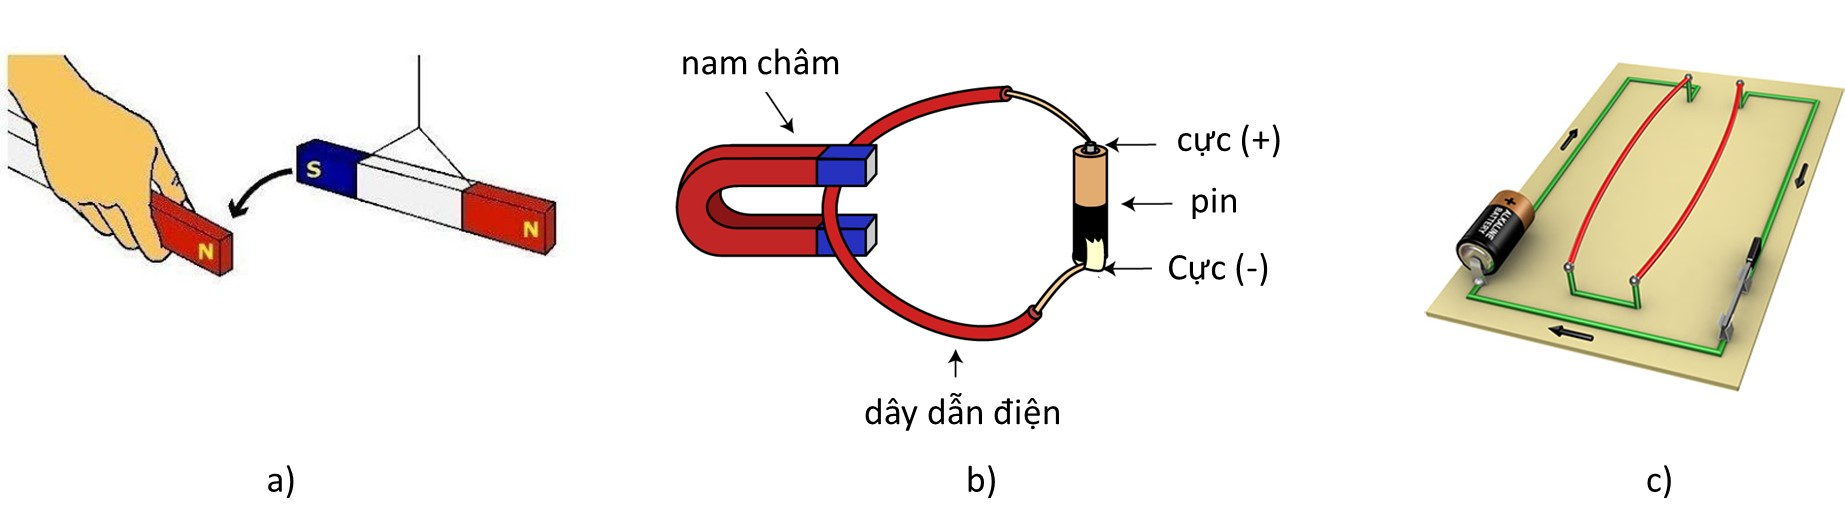
\includegraphics[width=0.9\linewidth]{figs/VN12-Y24-PH-SYL-017-1}
		\captionof{figure}{Tương tác từ giữa a) hai nam châm; b) nam châm với dòng điện; c) dòng điện với dòng điện.}
	\end{center}
	\subsubsection{Từ trường}
	\paragraph{Khái niệm từ trường}
	\begin{dn}
		Từ trường là trường lực gây ra bởi dòng điện hoặc nam châm, là một dạng của vật chất tồn tại xung quanh dòng điện hoặc nam châm mà biểu hiện cụ thể là sự xuất hiện của lực từ tác dụng lên một dòng điện hay một nam châm khác đặt trong nó.
	\end{dn}
	\paragraph{Từ phổ}
	\begin{dn}
		Từ phổ là hình ảnh tạo ra bởi các mạt sắt trong từ trường đang xét. Từ phổ cho thấy hình ảnh trực quan của từ trường.
	\end{dn}
	\begin{center}
		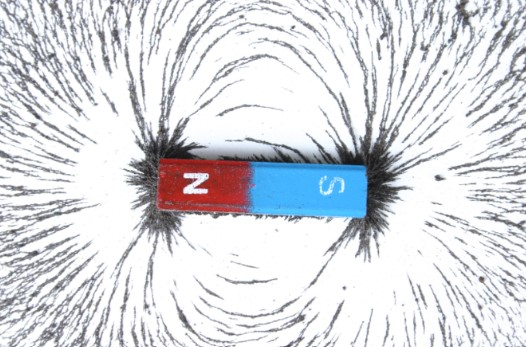
\includegraphics[width=0.4\linewidth]{figs/VN12-Y24-PH-SYL-017-2}
		\captionof{figure}{Từ phổ của một nam châm thẳng.}
	\end{center}
	\subsubsection{Cảm ứng từ}
	\paragraph{Khái niệm cảm ứng từ}
	\begin{dn}
		\begin{itemize}
			\item Để đặc trưng cho từ trường về mặt tác dụng lực, người ta đưa vào một đại lượng vector gọi là cảm ứng từ, kí hiệu là $\vec{B}$. 
			\item Phương của $\vec{B}$ là phương của nam châm thử nằm cân bằng tại một điểm trong từ trường.
			\item Chiều của $\vec{B}$ là chiều từ cực Nam sang Bắc của nam châm thử.
			\item Lực từ tác dụng lên một dòng điện (đoạn dây dẫn có dòng điện chạy qua) hay một nam châm đặt trong từ trường ở điểm nào lớn hơn thì cảm ứng từ tại điểm đó lớn hơn.
		\end{itemize}
	\end{dn}
	
	\paragraph{Đường sức từ}
	\begin{dn}
		Đường sức từ là những đường mô tả từ trường, sao cho tiếp tuyến tại bất kì điểm nào trên đường sức từ đều có phương, chiều trùng với phương, chiều của vector cảm ứng từ tại điểm đó.
	\end{dn}
	\begin{center}
		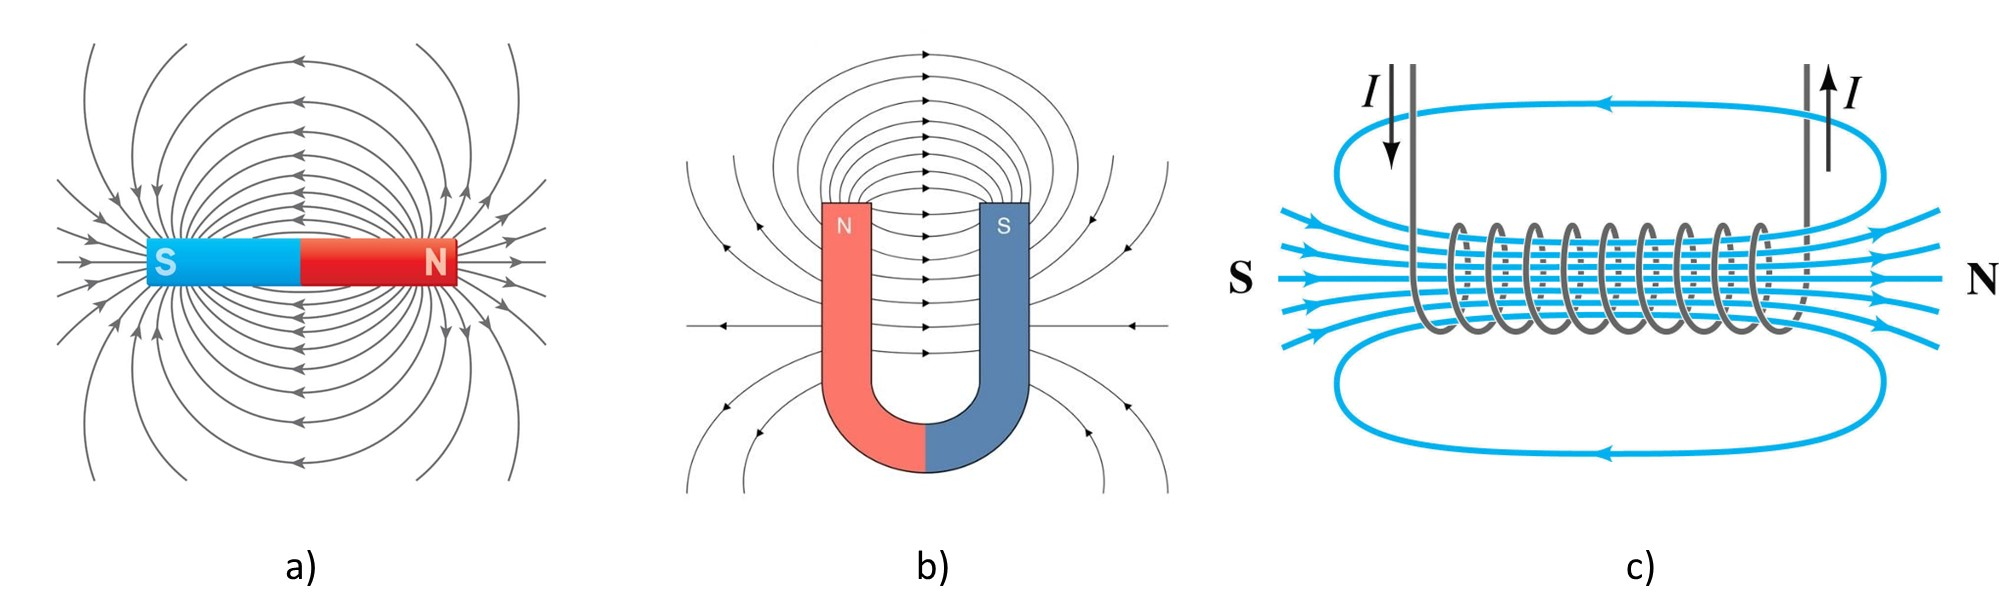
\includegraphics[width=0.85\linewidth]{figs/VN12-Y24-PH-SYL-017-3}
		\captionof{figure}{\textbf{Các đường sức từ của} a) nam châm thẳng; b) nam châm chữ U; c) ống dây có dòng điện chạy qua.}
	\end{center}
	\textbf{Tính chất của các đường sức từ:}
	\begin{tc}
		\begin{itemize}
			\item Tại mỗi điểm trong từ trường, có một và chỉ một đường sức từ đi qua điểm đó.
			\item Các đường sức từ là những đường cong kín. Đối với nam châm, các đường sức từ đi ra từ cực Bắc (N) và đi vào cực Nam (S).
			\item Nơi nào từ trường mạnh hơn thì các đường sức từ ở đó mau (dày) hơn, nơi nào từ trường yếu hơn thì các đường sức từ ở đó thưa hơn.
		\end{itemize}
	\end{tc}
	\paragraph{Từ trường đều}
	\begin{dn}
		Từ trường đều là từ trường có cảm ứng từ $\vec{B}$ tại mọi điểm đều bằng nhau.
	\end{dn}
	\textbf{\textit{Ví dụ:}} Vùng không gian giữa hai cực của nam châm chữ U có các đường sức từ gần như song song và cách đều nhau. Khi đó, từ trường giữa hai cực của nam châm chữ U được gọi là từ trường đều.
	\paragraph{Đường sức từ của một số dây dẫn đặc biệt}
	\begin{itemize}
		\item \textbf{Dòng điện thẳng}\\
		Đường sức từ của dòng điện điện thẳng là những đường tròn đồng tâm với tâm là giao điểm của đoạn dây dẫn và mặt phẳng.
		\begin{center}
			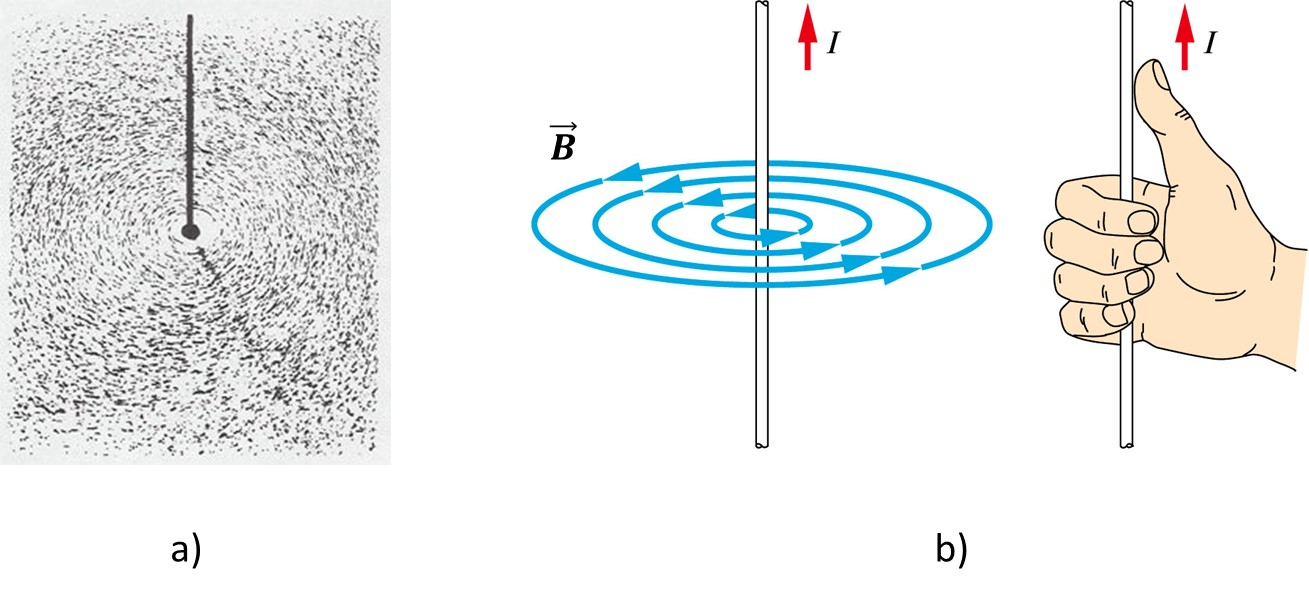
\includegraphics[width=0.6\linewidth]{{figs/VN12-Y24-PH-SYL-017-4}}
			\captionof{figure}{a) Từ phổ của dòng điện thẳng; b) Quy tắc nắm bàn tay phải để xác định chiều đường sức từ của dòng điện thẳng. }
		\end{center}
		\begin{noidung}{Quy tắc bàn tay phải để xác định chiều đường sức từ của dòng điện thẳng}
			Đặt bàn tay phải sao cho ngón cái hướng theo chiều dòng điện, khum các ngón tay còn lại xung quanh đoạn dây dẫn, khi đó chiều từ cổ tay đến các ngón tay chỉ chiều của đường sức từ.
		\end{noidung}
		\item \textbf{Dòng điện tròn}\\
		Đường sức từ tại những điểm nằm trên trục vòng dây của dòng điện tròn là đường thẳng.
		\begin{center}
			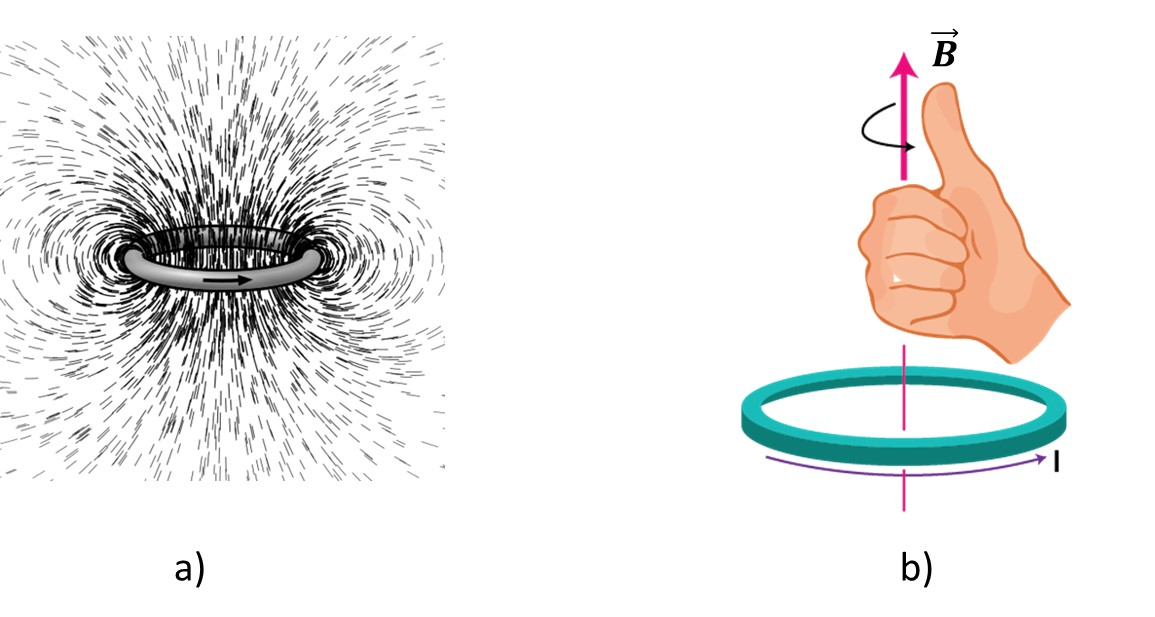
\includegraphics[width=0.6\linewidth]{figs/VN12-Y24-PH-SYL-017-5}
			\captionof{figure}{a) Từ phổ của dòng điện tròn, b) Quy tắc nắm tay phải để xác định chiều đường sức từ trên trục vòng dây của dòng điện tròn.}
		\end{center}
		\begin{noidung}{Quy tắc nắm tay phải để xác định chiều đường sức từ tại tâm của dòng điện tròn}
			Khum bàn tay phải theo vòng dây tròn sao cho chiều từ cổ tay đến các ngón tay trùng với chiều dòng điện trong dây dẫn; khi đó ngón cái choãi ra chỉ chiều của đường sức từ xuyên qua mặt phẳng dòng điện.
		\end{noidung}
		\item \textbf{Dòng điện trong ống dây}\\
		Đường sức từ tại những điểm nằm trên đường đi qua trục của ống dây là đường thẳng. Nếu chiều dài ống dây rất lớn so với bán kính các vòng dây, các đường sức từ bên trong ống dây sẽ song song và cách đều nhau. Một cách gần đúng, ta có thể xem từ trường bên trong ống dây là từ trường đều.
		\begin{center}
			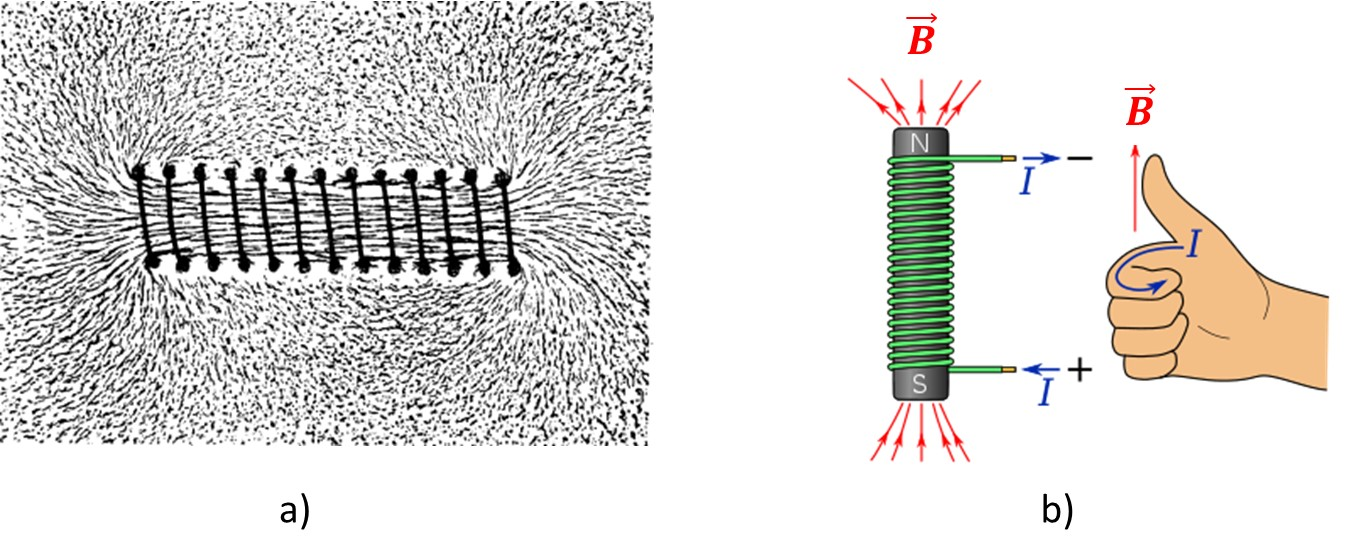
\includegraphics[width=0.6\linewidth]{figs/VN12-Y24-PH-SYL-017-6}
			\captionof{figure}{a) Từ phổ của dòng điện trong ống dây; b) Quy tắc nắm tay phải để xác định chiều của đường sức từ bên trong ống dây.}
		\end{center}
		\begin{noidung}{Quy tắc nắm tay phải để xác định chiều đường sức từ tại tâm của ống dây}
			Tưởng tượng dùng bàn tay phải nắm lấy ống dây sao cho các ngón trỏ, ngón giữa, \dots hướng theo chiều dòng điện; khi đó ngón cái choãi ra chỉ chiều của đường sức từ trong lòng ống dây.
		\end{noidung}
	\end{itemize}
\end{tomtat}
\subsection{Ví dụ minh họa}
\begin{dang}{Nêu được khái niệm từ trường và biểu hiện của từ trường}
\end{dang}
\begin{vd}
	Một học sinh có một nam châm đã biết vị trí cực Bắc và cực Nam. Để có thể sử dụng nam châm này xác định cực Bắc và cực Nam của các nam châm khác, học sinh này sẽ phải làm thế như nào?
	\loigiai{Đưa cực Bắc của nam châm đã biết lại gần một đầu của nam châm chưa xác định cực:
		\begin{itemize}
			\item nếu nam châm bị đẩy thì cực của nam châm chưa biết là cực Bắc.
			\item nếu nam châm bị hút thì cực của nam châm  chưa biết là cực Nam.
	\end{itemize}}
\end{vd}
\begin{vd}
	Đoạn dây dẫn AB căng thẳng mang điện tích. Nếu đưa một nam châm lại gần như hình thì đoạn dây AB có bị tác dụng bởi nam châm hay không? Giải thích.
	\begin{center}
		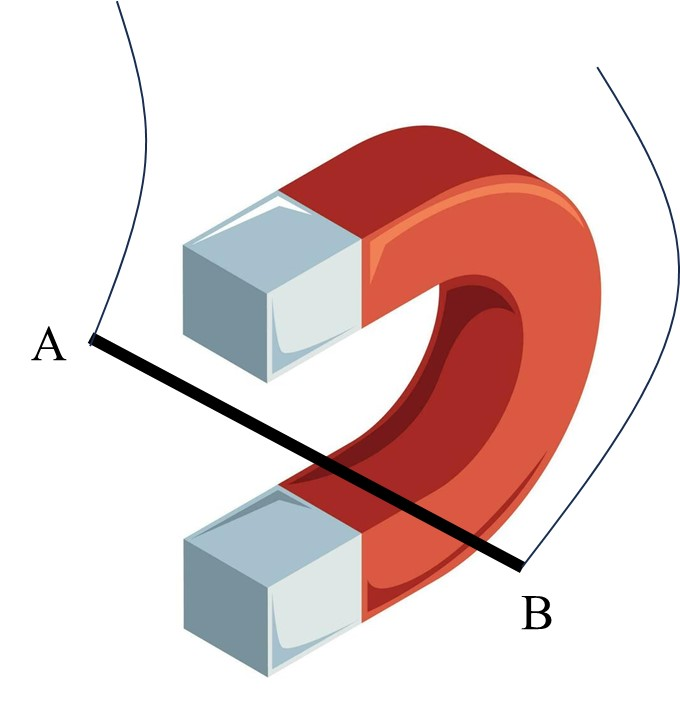
\includegraphics[width=0.25\linewidth]{figs/VN12-Y24-PH-SYL-017-7}
	\end{center}
	\loigiai{
	Đoạn dây AB không bị tác dụng bởi nam châm.\\
	Vì từ trường tác dụng lên dòng điện mà không tác dụng lên điện tích tĩnh.
	}
\end{vd}
\begin{dang}{Vận dụng quy tắc nắm tay phải để xác định chiều đường sức từ hoặc chiều dòng điện}
	\end{dang}
\begin{vd}
	Cho biết hình dạng và chiều của các đường sức từ như các hình vẽ. Xác định chiều của dòng điện chạy trong các dây dẫn ở các trường hợp sau:
	\begin{center}
		\begin{longtable}{M{8cm}M{8cm}}
			\begin{tikzpicture}[>=latex,line width=.7pt]
				\foreach \r in {1,2,3,4} 
				\draw[
				decoration={markings, mark=at position 0.125 with {\arrow{>}}},
				decoration={markings, mark=at position 0.625 with {\arrow{>}}},
				postaction={decorate}
				]
				(0,0) circle (\r/2);
			\end{tikzpicture}&
			\begin{tikzpicture}[>=latex,line width=.7pt]
				\node [cylinder, fill=gray!50, line width=1.5pt, shape border rotate=180, draw, minimum height=6.0cm, minimum width=1.0cm] at (4.5,0) {};
				\foreach \n in {1,2,3}
				\draw[
				decoration={markings, mark=at position 0.5 with {\arrow{>}}}, preaction={draw,white,line width=2pt}, postaction={decorate}
				]  (2*\n,0.5) arc (165:-165:0.5cm and 2cm);
			\end{tikzpicture}\\
			Hình a & Hình b
		\end{longtable}
	\end{center}
	\begin{note}
	Quy ước:
	\begin{itemize}
		\item $\otimes$ chiều dòng điện hướng vuông góc từ ngoài vào trong trang giấy.
		\item $\odot$ chiều dòng điện hướng vuông góc từ trong trang giấy ra ngoài.
	\end{itemize}
		\end{note}
		\loigiai{
		\begin{center}
			\begin{longtable}{M{8cm}M{8cm}}
				\begin{tikzpicture}[>=latex,line width=.7pt]
					\foreach \r in {1,2,3,4} 
					\draw[
					decoration={markings, mark=at position 0.125 with {\arrow{>}}},
					decoration={markings, mark=at position 0.625 with {\arrow{>}}},
					postaction={decorate}
					]
					(0,0) circle (\r/2);
					\draw[blue, line width=1.25pt] (0,0) circle (0.25);
					\filldraw[blue] (0,0) circle (2pt) ;
					\node [blue] at (0,0.65) {$I$};
				\end{tikzpicture}
				&
				\begin{tikzpicture}[>=latex,line width=.7pt]
					\node [cylinder, fill=gray!50, line width=1.5pt, shape border rotate=180, draw, minimum height=6.0cm, minimum width=1.0cm] at (4.5,0) {};
					\foreach \n in {1,2,3}
					\draw[
					decoration={markings, mark=at position 0.5 with {\arrow{>}}}, preaction={draw,white,line width=2pt}, postaction={decorate}
					]  (2*\n,0.5) arc (165:-165:0.5cm and 2cm);
					\draw[line width=1.25pt, blue, -latex] (7.4,0)--(9,0);
					\node[blue, above] at (9,0) {$I$};
				\end{tikzpicture}\\
				Hình a & Hình b
			\end{longtable}
		\end{center}
		}
\end{vd}
\begin{vd}
Hãy xác định cực của ống dây và cực của kim nam châm trong hai hình sau:\\
\begin{center}
	\begin{longtable}{M{8cm}M{8cm}}
		\begin{tikzpicture}		
			\def\coil#1{
				{0.2 * (2*#1 + \t) + 0.4*sin(\t * pi r))},
				{0.65 * cos(\t * pi r)}
			}
			
			% Draw the part of the coil behind the rectangle
			\foreach \n in {1,2,...,10} {
				\draw[domain={0:1},smooth,variable=\t,samples=100]
				plot (\coil{\n}); 
			}
			
			% Draw the cylinder
			\node [cylinder, fill=white, line width=1.5pt, shape border rotate=180, draw, minimum height=5.0cm, minimum width=1.0cm] at (2.15,0) {};
			% Draw the part of the coil in front of the rectangle
			\foreach \n in {0,1,...,9} {
				\draw[domain={1:2},smooth,variable=\t,samples=100,  
				preaction={draw,white,line width=2pt,}     % remove if undesired
				] 
				plot (\coil{\n});
				%	\node[rotate=80] at (-0.05+0.4*\n, 0) {>};
			}
			\draw[line width=0.8pt] (0.20,-0.65)--(0.20,-3)--(4.20,-3)--(4.20,-0.65);
			\node[draw, line width=1pt, fill=white, shape=rectangle, minimum width=1.5cm, minimum height=0.5cm, anchor=center] at (2.22,-3) {};
			\node[above] at (1.5,-2.75) {+};
			\node[above] at (3,-2.75) {-};
			\draw[line width=1pt](-2,-0.25)--(-2,0.25)--(-3,0)--(-2,-0.25);
			\draw[line width=1pt](-2,-0.25)--(-2,0.25)--(-1,0)--(-2,-0.25);
		\end{tikzpicture}
		&
		\begin{tikzpicture}		
			\def\coil#1{
				{0.2 * (2*#1 + \t) + 0.4*sin(\t * pi r))},
				{0.65 * cos(\t * pi r)}
			}
			
			% Draw the part of the coil behind the rectangle
			\foreach \n in {1,2,...,10} {
				\draw[domain={0:1},smooth,variable=\t,samples=100]
				plot (\coil{\n}); 
			}
			
			% Draw the cylinder
			\node [cylinder, fill=white, line width=1.5pt, shape border rotate=180, draw, minimum height=5.0cm, minimum width=1.0cm] at (2.15,0) {};
			% Draw the part of the coil in front of the rectangle
			\foreach \n in {0,1,...,9} {
				\draw[domain={1:2},smooth,variable=\t,samples=100,  
				preaction={draw,white,line width=2pt,}     % remove if undesired
				] 
				plot (\coil{\n});
				%	\node[rotate=80] at (-0.05+0.4*\n, 0) {>};
			}
			\draw[line width=0.8pt] (0.20,-0.65)--(0.20,-3)--(4.20,-3)--(4.20,-0.65);
			\node[draw, line width=1pt, fill=white, shape=rectangle, minimum width=1.5cm, minimum height=0.5cm, anchor=center] at (2.22,-3) {};
			\node[above] at (1.5,-2.75) {-};
			\node[above] at (3,-2.75) {+};
			\draw[line width=1pt](2,-1.5)--(2,-1.0)--(1,-1.25)--(2,-1.5);
			\draw[line width=1pt](2,-1.5)--(2,-1.0)--(3,-1.25)--(2,-1.5);
		\end{tikzpicture}\\
		Hình a & Hình b
	\end{longtable}
\end{center}
\loigiai{
\begin{center}
	\begin{longtable}{M{8cm}M{8cm}}
		\begin{tikzpicture}		
			\def\coil#1{
				{0.2 * (2*#1 + \t) + 0.4*sin(\t * pi r))},
				{0.65 * cos(\t * pi r)}
			}	
			% Draw the part of the coil behind the cylinder
			\foreach \n in {1,2,...,10} {
				\draw[domain={0:1},smooth,variable=\t,samples=100]
				plot (\coil{\n}); 
			}	
			% Draw the cylinder
			\node [cylinder, fill=white, line width=1.5pt, shape border rotate=180, draw, minimum height=5.0cm, minimum width=1.0cm] at (2.15,0) {};
			% Draw the part of the coil in front of the rectangle
			\foreach \n in {0,1,...,9} {
				\draw[domain={1:2},smooth,variable=\t,samples=100,  
				preaction={draw,white,line width=2pt,}     % remove if undesired
				] 
				plot (\coil{\n});
				\node[rotate=80] at (-0.1+0.4*\n, 0) {>};
			}
			\draw[line width=0.8pt] (0.20,-0.65)--(0.20,-3)--(4.20,-3)--(4.20,-0.65);
			\node[draw, line width=1pt, fill=white, shape=rectangle, minimum width=1.5cm, minimum height=0.5cm, anchor=center] at (2.22,-3) {};
			\node[above] at (1.5,-2.75) {+};
			\node[above] at (3,-2.75) {-};
			\draw[line width=1pt,fill=blue!75!black](-2,-0.25)--(-2,0.25)--(-3,0)--(-2,-0.25);
			\draw[line width=1pt](-2,-0.25)--(-2,0.25)--(-1,0)--(-2,-0.25);
		\end{tikzpicture}
		&
		\begin{tikzpicture}		
			
			\def\coil#1{
				{0.2 * (2*#1 + \t) + 0.4*sin(\t * pi r))},
				{0.65 * cos(\t * pi r)}
			}
			
			% Draw the part of the coil behind the rectangle
			\foreach \n in {1,2,...,10} {
				\draw[domain={0:1},smooth,variable=\t,samples=100]
				plot (\coil{\n}); 
			}
			
			% Draw the cylinder
			\node [cylinder, fill=white, line width=1.5pt, shape border rotate=180, draw, minimum height=5.0cm, minimum width=1.0cm] at (2.15,0) {};
			% Draw the part of the coil in front of the rectangle
			\foreach \n in {0,1,...,9} {
				\draw[domain={1:2},smooth,variable=\t,samples=100,  
				preaction={draw,white,line width=2pt,}     % remove if undesired
				] 
				plot (\coil{\n});
				\node[rotate=80] at (-0.1+0.4*\n, 0) {<};
			}
			\draw[line width=0.8pt] (0.20,-0.65)--(0.20,-3)--(4.20,-3)--(4.20,-0.65);
			\node[draw, line width=1pt, fill=white, shape=rectangle, minimum width=1.5cm, minimum height=0.5cm, anchor=center] at (2.22,-3) {};
			\node[above] at (1.5,-2.75) {-};
			\node[above] at (3,-2.75) {+};
			\draw[line width=1pt, fill=blue!75!black](2,-1.5)--(2,-1.0)--(1,-1.25)--(2,-1.5);
			\draw[line width=1pt](2,-1.5)--(2,-1.0)--(3,-1.25)--(2,-1.5);
		\end{tikzpicture}\\
		Hình a & Hình b
	\end{longtable}
\end{center}
}
\end{vd}

\begin{vd}
Hãy xác định cực của nguồn AB trong hai trường hợp sau:\\
\begin{center}
	\begin{longtable}{M{8cm}M{8cm}}
		\begin{tikzpicture}		
			\def\coil#1{
				{0.2 * (2*#1 + \t) + 0.4*sin(\t * pi r))},
				{0.65 * cos(\t * pi r)}
			}
			
			% Draw the part of the coil behind the rectangle
			\foreach \n in {1,2,...,10} {
				\draw[domain={0:1},smooth,variable=\t,samples=100]
				plot (\coil{\n}); 
			}
			
			% Draw the cylinder
			\node [cylinder, fill=white, line width=1.5pt, shape border rotate=180, draw, minimum height=5.0cm, minimum width=1.0cm] at (2.15,0) {};
			% Draw the part of the coil in front of the rectangle
			\foreach \n in {0,1,...,9} {
				\draw[domain={1:2},smooth,variable=\t,samples=100,  
				preaction={draw,white,line width=2pt,}     % remove if undesired
				] 
				plot (\coil{\n});
				%\node[rotate=70] at (-0.08+0.4*\n, 0) {<};
			}
			\draw[line width=0.8pt] (0.20,-0.65)--(0.20,-3)--(4.20,-3)--(4.20,-0.65);
			\node[draw, line width=1pt, fill=white, shape=rectangle, minimum width=1.5cm, minimum height=0.5cm, anchor=center] at (2.22,-3) {};
			\draw[line width=1pt, fill=blue!75!black](2,1)--(2,1.5)--(1,1.25)--(2,1);
			\draw[line width=1pt](2,1)--(2,1.5)--(3,1.25)--(2,1);
			\node[below] at (1.5,-3.25) {A};
			\node[below] at (3,-3.25) {B};
		\end{tikzpicture}
		&
		\begin{tikzpicture}		
			\def\coil#1{
				{0.2 * (2*#1 + \t) + 0.4*sin(\t * pi r))},
				{0.65 * cos(\t * pi r)}
			}
			
			% Draw the part of the coil behind the rectangle
			\foreach \n in {1,2,...,10} {
				\draw[domain={0:1},smooth,variable=\t,samples=100]
				plot (\coil{\n}); 
			}
			
			% Draw the cylinder
			\node [cylinder, fill=white, line width=1.5pt, shape border rotate=180, draw, minimum height=5.0cm, minimum width=1.0cm] at (2.15,0) {};
			% Draw the part of the coil in front of the rectangle
			\foreach \n in {0,1,...,9} {
				\draw[domain={1:2},smooth,variable=\t,samples=100,  
				preaction={draw,white,line width=2pt,}     % remove if undesired
				] 
				plot (\coil{\n});
				%	\node[rotate=70] at (-0.08+0.4*\n, 0) {<};
			}
			\draw[line width=0.8pt] (0.20,-0.65)--(0.20,-3)--(4.20,-3)--(4.20,-0.65);
			\node[draw, line width=1pt, fill=white, shape=rectangle, minimum width=1.5cm, minimum height=0.5cm, anchor=center] at (2.22,-3) {};
			\draw[line width=1pt](6,-0.25)--(6,0.25)--(5,0)--(6,-0.25);
			\draw[line width=1pt, fill=blue!75!black](6,-0.25)--(6,0.25)--(7,0)--(6,-0.25);
			\node[below] at (1.5,-3.25) {A};
			\node[below] at (3,-3.25) {B};
		\end{tikzpicture}\\
		Hình a & Hình b
	\end{longtable}
\end{center}
\loigiai{
	\begin{center}
		\begin{longtable}{M{8cm}M{8cm}}
			\begin{tikzpicture}	
				\def\coil#1{
					{0.2 * (2*#1 + \t) + 0.4*sin(\t * pi r))},
					{0.65 * cos(\t * pi r)}
				}
				
				% Draw the part of the coil behind the rectangle
				\foreach \n in {1,2,...,10} {
					\draw[domain={0:1},smooth,variable=\t,samples=100]
					plot (\coil{\n}); 
				}
				
				% Draw the cylinder
				\node [cylinder, fill=white, line width=1.5pt, shape border rotate=180, draw, minimum height=5.0cm, minimum width=1.0cm] at (2.15,0) {};
				% Draw the part of the coil in front of the rectangle
				\foreach \n in {0,1,...,9} {
					\draw[domain={1:2},smooth,variable=\t,samples=100,  
					preaction={draw,white,line width=2pt,}     % remove if undesired
					] 
					plot (\coil{\n});
					\node[rotate=80] at (-0.1+0.4*\n, 0) {<};
				}
				\draw[line width=0.8pt] (0.20,-0.65)--(0.20,-3)--(4.20,-3)--(4.20,-0.65);
				\node[draw, line width=1pt, fill=white, shape=rectangle, minimum width=1.5cm, minimum height=0.5cm, anchor=center] at (2.22,-3) {};
				\node[above] at (1.5,-2.75) {-};
				\node[above] at (3,-2.75) {+};
				\node[below] at (1.5,-3.25) {A};
				\node[below] at (3,-3.25) {B};
				\node[right,red] at (4.5,0) {N};
				\node[left,red] at (-0.4,0) {S};
				\draw[line width=1pt, fill=blue!75!black](2,1)--(2,1.5)--(1,1.25)--(2,1);
				\draw[line width=1pt](2,1)--(2,1.5)--(3,1.25)--(2,1);
			\end{tikzpicture}
			&
			\begin{tikzpicture}		
				\def\coil#1{
					{0.2 * (2*#1 + \t) + 0.4*sin(\t * pi r))},
					{0.65 * cos(\t * pi r)}
				}
				
				% Draw the part of the coil behind the rectangle
				\foreach \n in {1,2,...,10} {
					\draw[domain={0:1},smooth,variable=\t,samples=100]
					plot (\coil{\n}); 
				}
				
				% Draw the cylinder
				\node [cylinder, fill=white, line width=1.5pt, shape border rotate=180, draw, minimum height=5.0cm, minimum width=1.0cm] at (2.15,0) {};
				% Draw the part of the coil in front of the rectangle
				\foreach \n in {0,1,...,9} {
					\draw[domain={1:2},smooth,variable=\t,samples=100,  
					preaction={draw,white,line width=2pt,}     % remove if undesired
					] 
					plot (\coil{\n});
					\node[rotate=80] at (-0.1+0.4*\n, 0) {<};
				}
				
				\draw[line width=0.8pt] (0.20,-0.65)--(0.20,-3)--(4.20,-3)--(4.20,-0.65);
				\node[draw, line width=1pt, fill=white, shape=rectangle, minimum width=1.5cm, minimum height=0.5cm, anchor=center] at (2.22,-3) {};
				\node[above] at (1.5,-2.75) {-};
				\node[above] at (3,-2.75) {+};
				\node[below] at (1.5,-3.25) {A};
				\node[below] at (3,-3.25) {B};
				\node[right,red] at (4.5,0) {N};
				\node[left,red] at (-0.4,0) {S};
				\draw[line width=1pt](6,-0.25)--(6,0.25)--(5,0)--(6,-0.25);
				\draw[line width=1pt, fill=blue!75!black](6,-0.25)--(6,0.25)--(7,0)--(6,-0.25);
			\end{tikzpicture}\\
			Hình a & Hình b
		\end{longtable}
	\end{center}
}
\end{vd}
\subsection{Bài tập}
\subsubsection{Trắc nghiệm nhiều phương án lựa chọn}
\setcounter{ex}{0}
\Opensolutionfile{ans}[ans/VN12-Y24-PH-SYL-017P-TN]
% ===================================================================
\begin{ex}
	Một thanh nam châm bao giờ cũng có
	\choice
	{một loại cực từ}
	{\True hai loại cực từ}
	{ba loại cực từ}
	{một hoặc hai loại cực từ}
	\loigiai{}
\end{ex}
% ===================================================================
\begin{ex}
	Khi đưa cực từ bắc của thanh nam châm này lại gần cực từ nam của thanh nam châm kia thì
	\choice
	{\True chúng hút nhau}
	{tạo ra dòng điện}
	{chúng đẩy nhau}
	{chúng không hút nhau cũng không đẩy nhau}
	\loigiai{}
\end{ex}
% ===================================================================
\begin{ex}
	Sự sắp xếp kim nam châm ở hình nào sau đây là \textbf{đúng}?	
	\begin{center}
		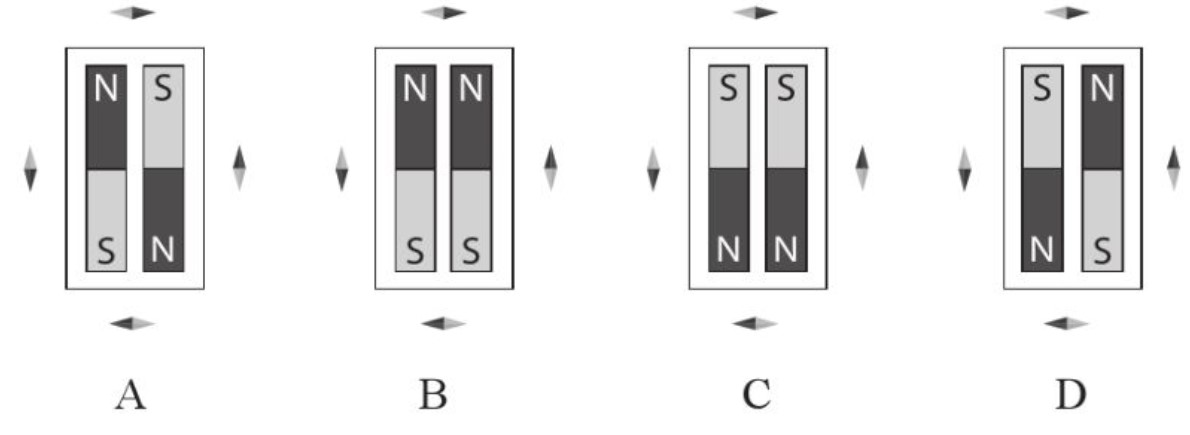
\includegraphics[width=0.7\linewidth]{figs/VN12-Y24-PH-SYL-017P-7}
	\end{center}
	\choice
	{\True A}
	{B}
	{C}
	{D}
	\loigiai{}
\end{ex}

% ===================================================================
\begin{ex}
	Tương tác từ \textbf{không} xảy ra trong trường hợp nào sau đây?
	\choice
	{Một thanh nam châm và một dòng điện không đổi đặt gần nhau}
	{Hai thanh nam châm đặt gần nhau}
	{\True Một thanh nam châm và một thanh đồng đặt gần nhau}
	{Một thanh nam châm và một thanh sắt non đặt gần nhau}
	\loigiai{}
\end{ex}
% ===================================================================
\begin{ex}
	Tính chất cơ bản của từ trường là
	\choice
	{\True gây ra lực từ tác dụng lên nam châm hoặc lên dòng điện đặt trong đó}
	{gây ra lực hấp dẫn lên các vật đặt trong đó}
	{gây ra lực đàn hồi tác dụng lên các dòng điện và nam châm đặt trong đó}
	{gây ra sự biến đổi về tính chất điện của môi trường xung quanh}
	\loigiai{}
\end{ex}
% ===================================================================
\begin{ex}
	Các đường sức từ	
	\choice
	{luôn cắt nhau}
	{\True không bao giờ cắt nhau}
	{luôn song song nhau}
	{có thể cắt nhau hoặc không}
	\loigiai{}
\end{ex}

% ===================================================================
\begin{ex}
	Xung quanh vật nào sau đây \textbf{không} có từ trường?	
	\choice
	{Dòng điện không đổi}
	{Hạt mang điện chuyển động}
	{\True Hạt mang điện đứng yên}
	{Nam châm hình chữ U}
	\loigiai{}
\end{ex}
% ===================================================================
\begin{ex}
	Trong các phát biểu sau, có bao nhiêu phát biểu \textbf{đúng}?	
	\begin{enumerate}[label=(\arabic*)]
		\item Mọi nam châm đều có hai cực: cực âm Nam (S) và cực Bắc  (N).
		\item Một số loài vật có thể sử dụng từ trường để tạo ra dòng điện làm tê liệt con mồi.
		\item Trái Đất là một nam châm khổng lồ, cực Bắc nam châm Trái Đất chính là cực Bắc địa lí và ngược lại.
		\item Cảm ứng từ là đại lượng đặc trưng cho từ trường về mặt năng lượng.
	\end{enumerate}
	\choice
	{\True 1}
	{2}
	{3}
	{4}
	\loigiai{Phát biểu đúng là (1).}
\end{ex}
% ===================================================================
\begin{ex}
	Chỉ ra câu \textbf{sai}.	
	\choice
	{Các đường mạt sắt của từ phổ cho biết dạng của đường sức từ}
	{Các đường sức từ của từ trường đều là những đường thẳng song song, cách đều nhau}
	{Nói chung các đường sức điện của điện tích đứng yên thì không kín, còn các đường sức từ là những đường cong kín}
	{\True Một hạt mang điện chuyển động theo quỹ đạo tròn trong từ trường thì quỹ đạo của nó là một đường sức từ của từ trường}
	\loigiai{}
\end{ex}
% ===================================================================
\begin{ex}
	Các đường sức từ xung quanh dây dẫn thẳng có dòng điện không đổi chạy qua có dạng là	
	\choice
	{những đường thẳng song song với dòng điện}
	{những đường thẳng vuông góc với dòng điện}
	{\True những vòng tròn đồng tâm với tâm nằm tại vị trí nơi dòng điện chạy qua}
	{những đường xoắn ốc đồng trục với trục là dòng điện}
	\loigiai{}
\end{ex}
% ===================================================================
\begin{ex}
	Từ phổ là
	\choice
	{\True hình ảnh của các đường mạt sắt cho ta hình ảnh của các đường sức từ của từ trường}
	{hình ảnh tương tác của hai nam châm với nhau}
	{hình ảnh tương tác giữa dòng điện và nam châm}
	{hình ảnh tương tác của hai dòng điện chạy trong hai dây dẫn thẳng song song}
	\loigiai{}
\end{ex}
% ===================================================================
\begin{ex}
	Phát biểu nào sau đây \textbf{không đúng}?	
	\choice
	{Qua bất kì điểm nào trong từ trường, ta cũng có thể vẽ được một đường sức từ}
	{\True Đường sức từ do nam châm thẳng tạo ra xung quanh nó là những đường thẳng}
	{Đường sức từ mau hơn ở nơi có từ trường lớn hơn, đường sức thưa hơn ở nơi có từ trường nhỏ hơn}
	{Các đường sức từ là những đường cong kín}
	\loigiai{}
\end{ex}
% ===================================================================
\begin{ex}
	Đặt một kim nam châm song song với dòng điện. Khi cho dòng điện chạy qua dây dẫn, ta thấy
	\choice
	{\True kim nam châm lệch một góc so với phương ban đầu}
	{kim nam châm đứng yên}
	{kim nam châm quay tròn xung quanh trục}
	{kim nam châm quay trái, quay phải liên tục}
	\loigiai{}
\end{ex}
% ===================================================================
\begin{ex}
	Phát biểu nào sau đây nói lên tính chất khác biệt của nam châm điện so với nam châm vĩnh cửu?
	\choice
	{Nam châm điện có cực từ bắc và cực từ nam}
	{Nam châm điện có thể hút các vật làm bằng vật liệu sắt từ}
	{\True Có thể bật hoặc tắt từ trường của nam châm điện}
	{Không thể đảo ngược được cực từ của nam châm điện}
	\loigiai{}
\end{ex}
% ===================================================================
\begin{ex}
	Một kim nam châm nhỏ nằm cân bằng tại một điểm trong từ trường. Hướng của từ trường tại điểm đó được quy ước là hướng	
	\choice
	{từ địa cực Bắc sang địa cực Nam của Trái Đất}
	{từ địa cực Nam sang địa cực Bắc của Trái Đất}
	{\True từ cực Nam sang cực Bắc của kim nam châm nhỏ}
	{từ cực Bắc sang cực Nam của kim nam châm nhỏ}
	\loigiai{}
\end{ex}


% ===================================================================
\begin{ex}
	Có hai thanh kim loại bằng sắt, bề ngoài giống nhau. Khi đặt chúng gần nhau thì chúng hút nhau. Kết luận nào sau đây về hai thanh đó là \textbf{đúng}?
	\choice
	{Đó là hai thanh nam châm}
	{Một thanh là nam châm, thanh còn lại là thanh sắt}
	{Có thể là hai thanh nam châm, cũng có thể là hai thanh sắt}
	{\True Có thể là hai thanh nam châm, cũng có thể là một thanh nam châm và một thanh sắt}
	\loigiai{}
\end{ex}
% ===================================================================
\begin{ex}
	Từ trường của một nam châm thẳng giống từ trường được tạo bởi
	\choice
	{một dây dẫn thẳng có dòng điện chạy qua}
	{\True một ống dây có dòng điện chạy qua}
	{một nam châm hình chữ U}
	{một vòng dây tròn có dòng điện chạy qua}
	\loigiai{}
\end{ex}
% ===================================================================
\begin{ex}
	Chọn ý \textbf{sai}. Người ta thường dùng nam châm điện thay cho nam châm vĩnh cửu là do
	\choice
	{nam châm điện có thể tạo ra từ trường mạnh/yếu tuỳ theo nhu cầu sử dụng}
	{nam châm vĩnh cửu tạo ra từ trường không đủ mạnh}
	{nam châm điện có thể thay đổi các cực của nam châm dễ dàng}
	{\True không thể dùng nam châm vĩnh cửu trong các ứng dụng hàng ngày}
	\loigiai{}
\end{ex}
% ===================================================================
\begin{ex}
	Một thanh nam châm được tách làm hai nửa. Chọn phát biểu \textbf{đúng}?
	\choice
	{Từ trường của mỗi mảnh rời nhau trở nên mạnh hơn}
	{Các cực từ được tách ra}
	{\True Hai thanh nam châm mới được tạo ra}
	{Điện trường được sinh ra}
	\loigiai{}
\end{ex}

% ===================================================================
\begin{ex}
	\immini{Cho một dòng điện thẳng, dài, đi qua một tấm bìa như hình vẽ bên. Dòng điện trong dây gây ra một từ trường xung quanh nó. Hình vẽ nào trong hình \ref{fig:17P-8} biểu diễn \textbf{đúng} chiều của các đường sức từ khi nhìn từ phía trên xuống?}
	{
		\begin{tikzpicture}[scale=0.5]
			\coordinate (O) at (0,0);
			\coordinate (A) at ($(O)+(45:3)$);
			\coordinate (C) at (4,0);
			\coordinate (B) at ($(C)+(45:3)$);
			\fill[orange!50!white, opacity=0.6] (O)--(A)--(B)--(C)--(O);
			\draw[line width=1.5pt, blue,decoration={markings, mark=at position 0.625 with {\arrowreversed{stealth}}},
			postaction={decorate}] 
			(3,1.45)--+(0,2);
			
			\draw[line width=1.5pt, blue] (3,0)--+(0,-1);
			\node[right] at (3,3) {$I$};
		\end{tikzpicture}
		%		\caption{}
		%		\label{fig:17P-7}
		
	}
	
	\begin{center}
		\begin{tabular}{cccc}
			\begin{tikzpicture}
				\coordinate (O) at (0,0);
				\foreach \i in {0, 45, ...,315}{
					\draw[line width=1pt, decoration={markings, mark=at position 0.5 with {\arrowreversed{stealth}}},
					postaction={decorate}] (O)--+(\i:2);}
				\node[circle, blue, fill=white, inner sep=0pt, minimum size=0pt] at (O) {$\LARGE\otimes$};
			\end{tikzpicture}
			
			&
			\begin{tikzpicture}
				\coordinate (O) at (0,0);
				\foreach \r in {1,2,3} {
					\draw[line width=1pt, decoration={markings, mark=at position 0 with {\arrow{stealth}}},
					postaction={decorate}
					]
					(0,0) circle (\r/2);	
				}
				\node[circle, blue, fill=white, inner sep=0pt, minimum size=0pt] at (O) {$\LARGE\otimes$};
			\end{tikzpicture}
			&
			\begin{tikzpicture}
				\coordinate (O) at (0,0);
				\foreach \i in {0, 45, ...,315}{
					\draw[line width=1pt, decoration={markings, mark=at position 0.625 with {\arrow{stealth}}},
					postaction={decorate}] (O)--+(\i:2);}
				\node[circle, blue, fill=white, inner sep=0pt, minimum size=0pt] at (O) {$\LARGE\otimes$};
			\end{tikzpicture}
			&
			\begin{tikzpicture}
				\coordinate (O) at (0,0);
				\foreach \r in {1,2,3} {
					\draw[line width=1pt, decoration={markings, mark=at position 0 with {\arrowreversed{stealth}}},
					postaction={decorate}
					]
					(0,0) circle (\r/2);	
				}
				\node[circle, blue, fill=white, inner sep=0pt, minimum size=0pt] at (O) {$\LARGE\otimes$};
			\end{tikzpicture}\\
			Hình a & Hình b & Hình c & Hình d
		\end{tabular}
		\captionof{figure}{}
		\label{fig:17P-8}
	\end{center}
	\choice
	{Hình a}
	{Hình b}
	{Hình c}
	{\True Hình d}
	\loigiai{}
\end{ex}
\Closesolutionfile{ans}

\subsubsection{Trắc nghiệm đúng/sai}
\Opensolutionfile{ans}[ans/VN12-Y24-PH-SYL-017P-TF]
\setcounter{ex}{0}
% ===================================================================
\begin{ex}
	Nhận xét nào sau đây là \textbf{không đúng} khi nói về tương tác từ giữa các vật?
	\choiceTF[t]
	{\True Dòng điện có thể tác dụng lực từ lên nam châm}
	{Nam châm thẳng không thể tác dụng lực từ lên nam châm chữ U}
	{\True Hai dòng diện có thể tương tác từ với nhau}
	{Hai dòng điện ngược chiều không thể tương tác với nhau}
	\loigiai{}
\end{ex}

% ===================================================================
\begin{ex}
	Cho hai nam châm thẳng đặt gần nhau và đối nhau:
	\choiceTF[t]
	{\True Nếu cực Bắc của một nam châm đối diện với cực Nam của nam châm kia, chúng sẽ hút nhau}
	{Nếu hai cực cùng cực đối diện, đường sức từ sẽ đi ra từ một nam châm và kết thúc ở nam châm kia}
	{\True Nếu hai cực Bắc của hai nam châm đặt đối diện nhau, các đường sức từ sẽ đẩy lẫn nhau tạo thành một khu vực không có đường sức từ giữa chúng}
	{Đưa hai cực của nam châm ra xa nhau, lực từ tương tác giữa chúng sẽ mạnh hơn so với khi chúng đặt gần nhau}
	\loigiai{}
\end{ex}
\begin{ex}
	Hình bên biểu diễn đường sức từ của hai nam châm thẳng đặt gần nhau. Từ hình cho biết:
	\begin{center}
		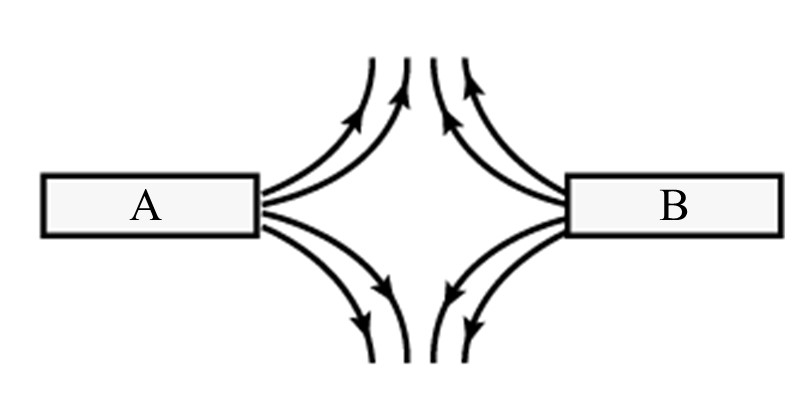
\includegraphics[width=0.35\linewidth]{figs/VN12-Y24-PH-SYL-017P-9}
	\end{center}
	\choiceTF[t]
	{Các cực Nam (S) hướng đối diện nhau}
	{Đường sức từ sẽ xuất phát từ điểm có từ trường mạnh nhất và kết thúc ở điểm có từ trường yếu nhất}
	{\True Khi hai nam châm cùng cực đặt đối diện nhau, đường sức từ sẽ bị biến dạng bởi vì sự tương tác giữa hai từ trường sẽ làm cho các đường sức từ bị uốn cong và hướng ra xa nhau}
	{Nếu các cực cùng tên của hai nam châm đặt đối diện nhau nhưng không chạm, ta có thể quan sát thấy một số đường sức từ chạm vào nhau tại điểm giữa hai nam châm}
	\loigiai{
		\begin{itemchoice}
			\itemch Các cực hướng đối diện nhau trong hình là cực Bắc.
			\itemch Các đường sức từ là các đường cong kín, không có điểm khởi đầu và kết thúc.
			\itemch Đúng.
			\itemch Các đường sức từ không cắt nhau.
		\end{itemchoice}
	}
	
\end{ex}
\Closesolutionfile{ans}
\subsubsection{Tự luận}
\setcounter{ex}{0}
\Opensolutionfile{ans}[ans/VN12-Y24-PH-SYL-017P-TL]
\begin{ex}
	Vẽ chiều của các đường sức từ tương ứng với nam châm thẳng, nam châm chữ U và dòng điện thẳng dài vô hạn trong các hình bên.
	\begin{center}
		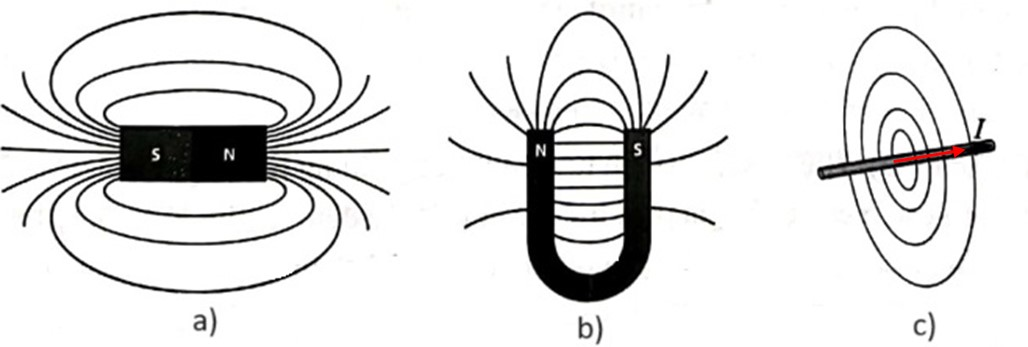
\includegraphics[width=0.8\linewidth]{figs/VN12-Y24-PH-SYL-017P-1}
	\end{center}
	\loigiai{
		\begin{center}
			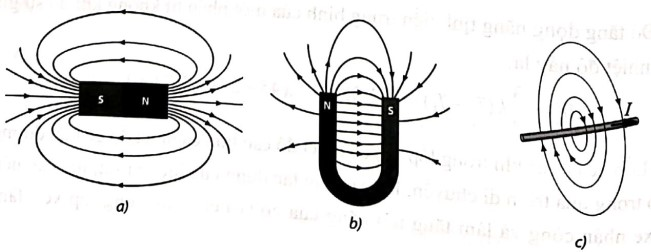
\includegraphics[width=0.6\linewidth]{figs/VN12-Y24-PH-SYL-017P-6}
		\end{center}
	}
\end{ex}

% ===================================================================
\begin{ex}
	Một cuộn dây dẫn được quấn quanh một lõi thép với hai đầu dây nối với nguồn điện không đổi như hình \ref{fig:17P-2}. Hãy vẽ chiều dòng điện trong mạch và vẽ phác các đường sức từ tạo bởi cuộn dây.
	\begin{center}
		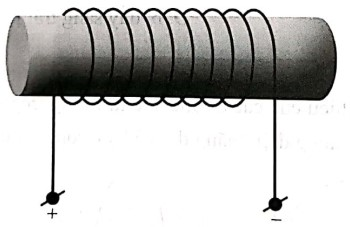
\includegraphics[width=0.3\linewidth]{figs/VN12-Y24-PH-SYL-017P-2}
		\captionof{figure}{}
		\label{fig:17P-2}
	\end{center}
	\loigiai{Chiều dòng điện trong mạch được thể hiện như hình bên. Dựa vào quy tắc nắm tay phải, ta xác định được chiều các đường sức từ tạo bởi ống dây.
		\begin{center}
			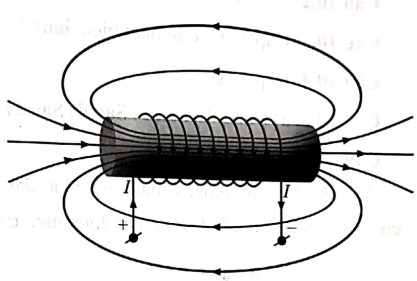
\includegraphics[width=0.4\linewidth]{figs/VN12-Y24-PH-SYL-017P-3}
	\end{center}}
\end{ex}
% ===================================================================
\begin{ex}
	Hiện nay, tàu đệm từ là một trong những phương tiện di chuyển với tốc độ cao ở các quốc gia phát triển. Xét một tàu đệm từ như hình \ref{fig:17P-4}, trong đó tàu được nâng lơ lửng trong không khí bằng hệ thống các nam châm điện. Ngoài ra, trên thân tàu và đường ray còn được gắn các nam châm điện khác đóng vai trò tăng tốc và giảm tốc cho tàu trong quá trình chuyển động.
	\begin{center}
		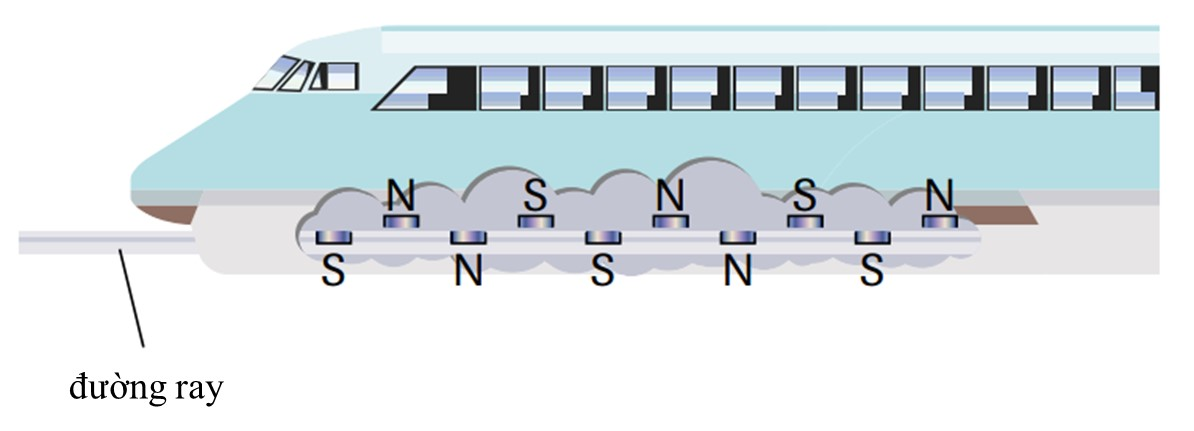
\includegraphics[width=0.6\linewidth]{figs/VN12-Y24-PH-SYL-017P-4}
		\captionof{figure}{}
		\label{fig:17P-4}
	\end{center}	
	\begin{enumerate}[label=\alph*)]
		\item Giả sử tại một thời điểm nào đó, cực từ của các nam châm được mô tả như trong hình, khi đó lực từ tổng hợp tác dụng lên tàu đệm từ đóng vai trò là lực đẩy hay lực cản chuyển động của tàu? Vì sao?
		\item Khi tàu sắp đến nhà ga và bắt đầu chuyển động chậm lại, khi đó chiều dòng điện chạy qua các nam châm điện cần thay đổi như thế nào?
	\end{enumerate}
	\loigiai{
		\begin{enumerate}[label=\alph*)]
			\item Xét bộ 3 nam châm liên tiếp nhau như hình bên. Sự tương tác giữa các cặp nam châm diễn ra như sau:
			\begin{center}
				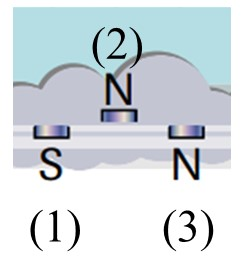
\includegraphics[width=0.15\linewidth]{figs/VN12-Y24-PH-SYL-017P-5}
			\end{center}
			\begin{itemize}
				\item Nam châm (1) hút nam chậm (2).
				\item Nam châm (3) đẩy nam châm (2).
			\end{itemize}
			Kết quả làm tàu đệm từ bị đẩy về phía trước. Điều tương tự xảy ra cho các bộ 3 nam châm liên tiếp nhau còn lại. Do đó, lực từ lúc này đóng vai trò là lực đẩy.
			\item Để tàu đệm từ giảm tốc độ, lực từ phải đóng vai trò là lực cản. Muốn vậy, dòng điện chạy qua bộ 3 nam châm điện liên tiếp nhau trong hình vẽ trên phải đổi chiều sao cho: nam châm (1) đẩy nam châm (2); nam châm (3) hút nam châm (2).
		\end{enumerate}	
	}
\end{ex}
% ===================================================================
\begin{ex}
	Hãy xác định cực của các kim nam châm trong hình \ref{fig:17P-6}.\\
	\begin{center}
		\begin{tabular}{ccc}
			\begin{tikzpicture}[scale=0.75]		
				
				\def\coil#1{
					{0.2 * (2*#1 + \t) + 0.4*sin(\t * pi r))},
					{0.65 * cos(\t * pi r - pi r)}
				}
				
				% Draw the part of the coil behind the rectangle
				\foreach \n in {0,1,2,...,9} {
					\draw[domain={0:1},smooth,variable=\t,samples=100]
					plot (\coil{\n}); 
				}
				
				% Draw the cylinder
				\node [cylinder, fill=white, line width=1.5pt, shape border rotate=180, draw, minimum height=5.0cm, minimum width=1.0cm, scale=0.75] at (2.15,0) {};
				% Draw the part of the coil in front of the rectangle
				\foreach \n in {0,1,...,9} {
					\draw[domain={1:2},smooth,variable=\t,samples=100,  
					preaction={draw,white,line width=2pt,}     % remove if undesired
					] 
					plot (\coil{\n});
					%	\node[rotate=80] at (-0.05+0.4*\n, 0) {>};
				}
				\draw[line width=0.8pt] (0,-0.65)--(0,-3)--(4,-3)--(4,-0.65);
				\node[draw, line width=1pt, fill=white, shape=rectangle, minimum width=1.5cm, minimum height=0.5cm, anchor=center] at (2.22,-3) {};
				\node[above] at (1.5,-2.75) {+};
				\node[above] at (3,-2.75) {-};
				\draw[line width=1pt](-2,-0.25)--(-2,0.25)--(-3,0)--(-2,-0.25);
				\draw[line width=1pt](-2,-0.25)--(-2,0.25)--(-1,0)--(-2,-0.25);
				\node[below] at (2,-3.5) {a)};
			\end{tikzpicture}
			&
			\begin{tikzpicture}[scale=0.75]		
				\def\coil#1{
					{0.2 * (2*#1 + \t) + 0.4*sin(\t * pi r))},
					{0.65 * cos(\t * pi r - pi r)}
				}
				
				% Draw the part of the coil behind the rectangle
				\foreach \n in {0,1,2,...,9} {
					\draw[domain={0:1},smooth,variable=\t,samples=100]
					plot (\coil{\n}); 
				}
				
				% Draw the cylinder
				\node [cylinder, fill=white, line width=1.5pt, shape border rotate=180, draw, minimum height=5.0cm, minimum width=1.0cm, scale=0.75] at (2.15,0) {};
				% Draw the part of the coil in front of the rectangle
				\foreach \n in {0,1,...,9} {
					\draw[domain={1:2},smooth,variable=\t,samples=100,  
					preaction={draw,white,line width=2pt,}     % remove if undesired
					] 
					plot (\coil{\n});
					%	\node[rotate=80] at (-0.05+0.4*\n, 0) {>};
				}
				\draw[line width=0.8pt] (0,-0.65)--(0,-3)--(4,-3)--(4,-0.65);
				\node[draw, line width=1pt, fill=white, shape=rectangle, minimum width=1.5cm, minimum height=0.5cm, anchor=center] at (2.22,-3) {};
				\node[above] at (1.5,-2.75) {-};
				\node[above] at (3,-2.75) {+};
				\draw[line width=1pt](2,-1)--(2,-1.5)--(1,-1.25)--(2,-1);
				\draw[line width=1pt](2,-1)--(2,-1.5)--(3,-1.25)--(2,-1);
				\node[below] at (2,-3.5) {b)};
			\end{tikzpicture}
			&
			\begin{tikzpicture}	[scale=0.75]	
				\def\coil#1{
					{0.2 * (2*#1 + \t) + 0.4*sin(\t * pi r))},
					{0.65 * cos(\t * pi r)}
				}
				
				% Draw the part of the coil behind the rectangle
				\foreach \n in {1,2,...,10} {
					\draw[domain={0:1},smooth,variable=\t,samples=100]
					plot (\coil{\n}); 
				}
				
				% Draw the cylinder
				\node [cylinder, fill=white, line width=1.5pt, shape border rotate=180, draw, minimum height=5.0cm, minimum width=1.0cm, scale=0.75] at (2.15,0) {};
				% Draw the part of the coil in front of the rectangle
				\foreach \n in {0,1,...,9} {
					\draw[domain={1:2},smooth,variable=\t,samples=100,  
					preaction={draw,white,line width=2pt,}     % remove if undesired
					] 
					plot (\coil{\n});
					%	\node[rotate=80] at (-0.05+0.4*\n, 0) {>};
				}
				\draw[line width=0.8pt] (0.2,-0.65)--(0.2,-3)--(4.2,-3)--(4.2,-0.65);
				\node[draw, line width=1pt, fill=white, shape=rectangle, minimum width=1.5cm, minimum height=0.5cm, anchor=center] at (2.22,-3) {};
				\node[above] at (1.5,-2.75) {+};
				\node[above] at (3,-2.75) {-};
				\draw[line width=1pt](2,1.5)--(2,1)--(1,1.25)--(2,1.5);
				\draw[line width=1pt](2,1.5)--(2,1)--(3,1.25)--(2,1.5);
				\node[below] at (2,-3.5) {c)};
			\end{tikzpicture}
		\end{tabular}
		\captionof{figure}{}
		\label{fig:17P-6}
	\end{center}
	\loigiai{\begin{center}
			\begin{tabular}{ccc}
				\begin{tikzpicture}[scale=0.75]		
					
					\def\coil#1{
						{0.2 * (2*#1 + \t) + 0.4*sin(\t * pi r))},
						{0.65 * cos(\t * pi r - pi r)}
					}
					
					% Draw the part of the coil behind the rectangle
					\foreach \n in {0,1,2,...,9} {
						\draw[domain={0:1},smooth,variable=\t,samples=100]
						plot (\coil{\n}); 
					}
					
					% Draw the cylinder
					\node [cylinder, fill=white, line width=1.5pt, shape border rotate=180, draw, minimum height=5.0cm, minimum width=1.0cm, scale=0.75] at (2.15,0) {};
					% Draw the part of the coil in front of the rectangle
					\foreach \n in {0,1,...,9} {
						\draw[domain={1:2},smooth,variable=\t,samples=100,  
						preaction={draw,white,line width=2pt,}     % remove if undesired
						] 
						plot (\coil{\n});
						%	\node[rotate=80] at (-0.05+0.4*\n, 0) {>};
					}
					\draw[line width=0.8pt] (0,-0.65)--(0,-3)--(4,-3)--(4,-0.65);
					\node[draw, line width=1pt, fill=white, shape=rectangle, minimum width=1.5cm, minimum height=0.5cm, anchor=center] at (2.22,-3) {};
					\node[above] at (1.5,-2.75) {+};
					\node[above] at (3,-2.75) {-};
					\draw[line width=1.5pt](-2,-0.25)--(-2,0.25)--(-1,0)--(-2,-0.25);
					\fill[blue, line width=1pt](-2,-0.25)--(-2,0.25)--(-1,0)--(-2,-0.25);
					\draw[line width=1pt](-2,-0.25)--(-2,0.25)--(-3,0)--(-2,-0.25);
					\node[below] at (2,-3.5) {a)};
				\end{tikzpicture}
				&
				\begin{tikzpicture}[scale=0.75]		
					\def\coil#1{
						{0.2 * (2*#1 + \t) + 0.4*sin(\t * pi r))},
						{0.65 * cos(\t * pi r - pi r)}
					}
					
					% Draw the part of the coil behind the rectangle
					\foreach \n in {0,1,2,...,9} {
						\draw[domain={0:1},smooth,variable=\t,samples=100]
						plot (\coil{\n}); 
					}
					
					% Draw the cylinder
					\node [cylinder, fill=white, line width=1.5pt, shape border rotate=180, draw, minimum height=5.0cm, minimum width=1.0cm, scale=0.75] at (2.15,0) {};
					% Draw the part of the coil in front of the rectangle
					\foreach \n in {0,1,...,9} {
						\draw[domain={1:2},smooth,variable=\t,samples=100,  
						preaction={draw,white,line width=2pt,}     % remove if undesired
						] 
						plot (\coil{\n});
						%	\node[rotate=80] at (-0.05+0.4*\n, 0) {>};
					}
					\draw[line width=0.8pt] (0,-0.65)--(0,-3)--(4,-3)--(4,-0.65);
					\node[draw, line width=1pt, fill=white, shape=rectangle, minimum width=1.5cm, minimum height=0.5cm, anchor=center] at (2.22,-3) {};
					\node[above] at (1.5,-2.75) {-};
					\node[above] at (3,-2.75) {+};
					\draw[line width=1pt](2,-1)--(2,-1.5)--(1,-1.25)--(2,-1);
					\draw[line width=1pt](2,-1)--(2,-1.5)--(3,-1.25)--(2,-1);
					\fill[blue](2,-1)--(2,-1.5)--(3,-1.25)--(2,-1);
					\node[below] at (2,-3.5) {b)};
				\end{tikzpicture}
				&
				\begin{tikzpicture}	[scale=0.75]	
					\def\coil#1{
						{0.2 * (2*#1 + \t) + 0.4*sin(\t * pi r))},
						{0.65 * cos(\t * pi r)}
					}
					
					% Draw the part of the coil behind the rectangle
					\foreach \n in {1,2,...,10} {
						\draw[domain={0:1},smooth,variable=\t,samples=100]
						plot (\coil{\n}); 
					}
					
					% Draw the cylinder
					\node [cylinder, fill=white, line width=1.5pt, shape border rotate=180, draw, minimum height=5.0cm, minimum width=1.0cm, scale=0.75] at (2.15,0) {};
					% Draw the part of the coil in front of the rectangle
					\foreach \n in {0,1,...,9} {
						\draw[domain={1:2},smooth,variable=\t,samples=100,  
						preaction={draw,white,line width=2pt,}     % remove if undesired
						] 
						plot (\coil{\n});
						%	\node[rotate=80] at (-0.05+0.4*\n, 0) {>};
					}
					\draw[line width=0.8pt] (0.2,-0.65)--(0.2,-3)--(4.2,-3)--(4.2,-0.65);
					\node[draw, line width=1pt, fill=white, shape=rectangle, minimum width=1.5cm, minimum height=0.5cm, anchor=center] at (2.22,-3) {};
					\node[above] at (1.5,-2.75) {+};
					\node[above] at (3,-2.75) {-};
					\draw[line width=1pt](2,1.5)--(2,1)--(1,1.25)--(2,1.5);
					\draw[line width=1pt](2,1.5)--(2,1)--(3,1.25)--(2,1.5);
					\fill[blue](2,1.5)--(2,1)--(3,1.25)--(2,1.5);
					\node[below] at (2,-3.5) {c)};
				\end{tikzpicture}
			\end{tabular}
	\end{center}}
\end{ex}


\Closesolutionfile{ans}


\newpage
%	\section{Lực từ - Cảm ứng từ}
\subsection{Tóm tắt lí thuyết}
\begin{tomtat}
	\subsubsection{Độ lớn cảm ứng từ}
	\begin{dn}
		Cảm ứng từ $\vec{B}$ là một đại lượng vector, đặc trưng cho từ trường về phương diện tác dụng lực. Cảm ứng từ tại một điểm trong từ trường có:
		\begin{itemize}
			\item Phương trùng với phương của nam châm thử nằm cân bằng tại điểm đó.
			\item Chiều từ cực  Nam sang cực Bắc của nam châm thử.
			\item Độ lớn được xác định bằng biểu thức:
			\begin{equation}
				B=\dfrac{F}{IL\sin\theta}
			\end{equation}
		\end{itemize}
	\end{dn}
	Trong hệ SI, cảm ứng từ có đơn vị là tesla $\left(\si{\tesla}\right)$. Đơn vị tesla là đơn vị dẫn xuất, có mối liên hệ với các đơn vị cơ bản theo biểu thức:
	\begin{equation}
		\SI{1}{\tesla}=\SI{1}{\dfrac{\newton}{\ampere\cdot\meter}}
	\end{equation}
	$\SI{1}{\tesla}$ là độ lớn của cảm ứng từ của một từ trường đều mà khi đặt một dây dẫn có chiều dài $\SI{1}{\meter}$ mang dòng điện có cường độ $\SI{1}{\ampere}$ vào trong từ trường đó và vuông góc với vector cảm ứng từ thì dây dẫn sẽ chịu một lực từ có độ lớn $\SI{1}{\newton}$.
	\subsubsection{Lực từ tác dụng lên đoạn dây dẫn mang dòng điện}
	\paragraph{Độ lớn lực từ}
	\begin{boxdl}
			Lực từ tác dụng lên một đoạn dây dẫn mang dòng điện đặt trong từ trường đều được tính bởi biểu thức:
		\begin{equation}
			F=ILB\sin\theta
		\end{equation}
	\end{boxdl}

	\begin{center}
		\begin{tikzpicture}
			\coordinate (O) at(0,0);
			\coordinate (A) at($(O)+(30:3)$);
			\coordinate (B) at($(O)+(-60:3)$);
			\coordinate (C) at(2.5,0);
			\tkzMarkRightAngle[size=0.7,color=blue, line width=1.5pt](B,O,C);
			\node [cylinder, fill=gray!30!white, line width=1pt, shape border rotate=180, draw, minimum height=8.0cm, minimum width=0.6cm] at (O) {};
			\draw[-stealth,line width=2pt, red] (-2,0)--(3,0);
			\tkzMarkRightAngle[size=0.4,color=blue, line width=1.5pt](B,O,A);
			\draw[-stealth, line width=2pt] (O)--(A);
			\draw[-stealth, line width=2pt] (O)--(B);
			\fill   (O) circle[radius=3pt];
			\node[above] at (A) {$\vec{B}$};
			\node[below] at ($(C)-(0,0.3)$) {$\vec{IL}$};
			\node[right] at (B) {$\vec{F}$};
			\tkzMarkAngle[size=0.75cm,color=purple, line width=1.5pt](C,O,A);
			\tkzLabelAngle[color=black,pos=1.2](C,O,A){$\theta$};
		\end{tikzpicture}
	\end{center}
	trong đó:
	\begin{itemize}
		\item $F$: độ lớn lực từ tác dụng lên đoạn dây, đơn vị trong hệ SI là $\left(\si{\meter}\right)$;
		\item $B$: độ lớn cảm ứng từ, đơn vị trong hệ SI là $\left(\si{\tesla}\right)$;
		\item $I$: cường độ dòng điện qua đoạn dây, đơn vị trong hệ SI là $\left(\si{\ampere}\right)$;
		\item $L$: chiều dài đoạn dây, đơn vị trong hệ SI là $\left(\si{\meter}\right)$;
		\item $\theta$: góc hợp bởi vector $\vec{B}$ và vector phần tử dòng điện $\vec{IL}$.
	\end{itemize}
	\paragraph{Phương và chiều của lực từ}
	Lực từ tác dụng lên đoạn dây dẫn mang dòng điện trong từ trường đều có:
	\begin{itemize}
		\item Điểm đặt là tại trung điểm của đoạn dây.
		\item Phương vuông góc với mặt phẳng chứa đoạn dây dẫn mang dòng điện và vector cảm ứng từ.
		\item Chiều được xác định bằng quy tắc bàn tay trái:\\
		Đặt bàn tay trái sao cho các đường sức từ hướng vào lòng bàn tay, chiều từ cổ tay đến các ngón tay trùng với chiều dòng điện, khi đó ngón cái choãi ra $\SI{90}{\degree}$ chỉ chiều của lực từ tác dụng lên dòng điện.
		\begin{center}
			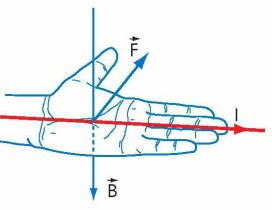
\includegraphics[width=0.3\linewidth]{figs/VN12-Y24-PH-SYL-017-8}
			\captionof{figure}{Hình vẽ mô tả quy tắc bàn tay trái.}
		\end{center}
	\end{itemize}
\end{tomtat}


\subsection{Ví dụ minh hoạ}
\begin{dang}{Vận dụng quy tắc bàn tay trái để xác định lực từ tác dụng đoạn dây dẫn mang dòng điện}
	\end{dang}
\begin{vd}
	Với mỗi trường hợp như hình, hãy xác định xem có lực từ tác dụng lên mỗi dây dẫn mang dòng điện hay không? Nếu có, hãy cho biết hướng của chúng.
	\begin{center}
		\begin{longtable}{M{8cm}M{8cm}}
			\begin{tikzpicture}
				\foreach \i in {0,1,...,4}
				\draw[blue, line width=1pt, decoration={markings, mark=at position 0.75 with {\arrow{stealth}}}, postaction={decorate}] (0, \i)--(5,\i);
				\node[right] at (5,4) {$\vec{B}$};
				\node[right, red] at (2.75,2.5) {$I$};
				\node[red] at (2.5,2.5) {\LARGE$\odot$};
			\end{tikzpicture}
			&
			\begin{tikzpicture}
				\foreach \i in {0,1,...,4}
				\draw[blue, line width=1pt, decoration={markings, mark=at position 0.75 with {\arrow{stealth}}}, postaction={decorate}] (0, \i)--(5,\i);
				\node[right] at (5,4) {$\vec{B}$};
				\node[right, red] at (2.75,1.8) {$I$};
				\draw[red, line width=1.5pt, decoration={markings, mark=at position 0.5 with {\arrow{stealth}}}, postaction={decorate}] (2.5, -0.5)--(2.5,4.5);
			\end{tikzpicture}\\
			Hình a & Hình b
		\end{longtable}
	\end{center}
	\loigiai{
		\begin{center}
			\begin{longtable}{M{8cm}M{8cm}}
				\begin{tikzpicture}
					\foreach \i in {0,1,...,4}
					\draw[blue, line width=1pt, decoration={markings, mark=at position 0.75 with {\arrow{stealth}}}, postaction={decorate}] (0, \i)--(5,\i);
					\node[right] at (5,4) {$\vec{B}$};
					\node[right, red] at (2.75,2.5) {$I$};
					\node[red] at (2.5,2.5) {\LARGE$\odot$};
					\draw[line width=1.5pt, green!75!black, -latex] (2.5,2.65)--(2.5,4.5);
					\node[right, green!75!black] at (2.5,4.5) {$\vec{F}$};
				\end{tikzpicture}
				&
				\begin{tikzpicture}
					\foreach \i in {0,1,...,4}
					\draw[blue, line width=1pt, decoration={markings, mark=at position 0.65 with {\arrow{stealth}}}, postaction={decorate}] (0, \i)--(5,\i);
					\node[right] at (5,4) {$\vec{B}$};
					\node[right, red] at (2.75,3.55) {$I$};
					\draw[red, line width=1.5pt, decoration={markings, mark=at position 0.65 with {\arrow{stealth}}}, postaction={decorate}] (2.5, -0.5)--(2.5,5.5);
					\node[green!75!black, fill=white] at(2.5,2.0) {\LARGE$\otimes$};
					\node[right, green!75!black] at (2.75,2.25) {$\vec{F}$};
				\end{tikzpicture}\\
				Hình a & Hình b
			\end{longtable}
		\end{center}
	}
\end{vd}

\begin{vd}
	Xác định chiều của dòng điện trong các hình bên dưới.
\begin{center}
		\begin{longtable}{M{8cm}M{8cm}}
		\begin{tikzpicture}
			\foreach \x in {0,1,...,3}{
				\foreach \y in {0,1,...,3}{
					\node[blue] at (\x,\y) {\LARGE$\odot$};}}
			\draw[line width=1.5pt, -latex] (1.5,1.5)--(1.5,3);
			\node[above] at (1.5,3) {$\vec{F}$};
			\node[right] at (3.1,2) {$\vec{B}$};
			\filldraw[black] (1.5,1.5) circle (2pt);
		\end{tikzpicture}
		&
		\begin{tikzpicture}
			\foreach \x in {0,1,...,3}{
				\foreach \y in {0,1,...,3}{
					\node[blue] at (\x,\y) {\LARGE$\otimes$};}}
			\draw[line width=1.5pt, -latex] (1.5,1.5)--(0,1.5);
			\node[left] at (0,1.5) {$\vec{F}$};
			\node[right] at (3.1,2) {$\vec{B}$};
			\filldraw[black] (1.5,1.5) circle (2pt);
		\end{tikzpicture}\\
		Hình a & Hình b
	\end{longtable}
\end{center}
\loigiai{
	\begin{center}
		\begin{longtable}{M{8cm}M{8cm}}
			\begin{tikzpicture}
				\foreach \x in {0,1,...,3}{
					\foreach \y in {0,1,...,3}{
						\node[blue] at (\x,\y) {\LARGE$\odot$};}}
				\draw[line width=1.5pt, -latex] (1.5,1.5)--(1.5,3);
				\draw[line width=1.5pt,red, -latex] (1.5,1.5)--(0,1.5);
				\node[above] at (1.5,3) {$\vec{F}$};
				\node[left,red] at (0,1.5) {$I$};
				\node[right] at (3.1,2) {$\vec{B}$};
				\filldraw[black] (1.5,1.5) circle (2pt);
			\end{tikzpicture}
			&
			\begin{tikzpicture}
				\foreach \x in {0,1,...,3}{
					\foreach \y in {0,1,...,3}{
						\node[blue] at (\x,\y) {\LARGE$\otimes$};}}
				\draw[line width=1.5pt, -latex] (1.5,1.5)--(0,1.5);
				\node[left] at (0,1.5) {$\vec{F}$};
				\node[right] at (3.1,2) {$\vec{B}$};
				\draw[line width=1.5pt,red, -latex] (1.5,1.5)--(1.5,3);
				\node[above,red] at (1.5,3) {$I$};
				\filldraw[black] (1.5,1.5) circle (2pt);
			\end{tikzpicture}\\
			Hình a & Hình b
		\end{longtable}
	\end{center}}
\end{vd}
\begin{dang}{Vận dụng được biểu thức tính độ lớn lực từ }
	Lực từ tác dụng lên đoạn dây dẫn chiều dài $L$ đặt trong từ trường đều $B$ có dòng điên $I$ chạy qua:
	$$F=ILB\sin\theta.$$
	\end{dang}
\begin{vd}
	Một dòng điện có cường độ $\SI{0.6}{\ampere}$ chạy dọc theo dây dẫn bằng đồng được uốn thành khung hình tam giác ABC như hình vẽ. Khung được đặt trong từ trường đều có cảm ứng từ $\SI{2.8E-4}{\tesla}$. Xác định lực từ tác dụng lên cạnh:
	\begin{center}
		\begin{tikzpicture}
			\foreach \i in {0,1,...,5}
			\draw[blue, line width=1pt, decoration={markings, mark=at position 0.15 with {\arrow{stealth}}}, postaction={decorate}] (0, -0.5+\i)--(6,-0.5+\i);
			\coordinate (A) at (1.5,0);
			\coordinate (B) at (1.5,4);
			\coordinate (C) at (4.5,4);
			\coordinate (D) at (1.7,0);
			\draw[line width=1.5pt] (A)--(B)--(C)--(D)--($(D)-(0,0.5)$);
			\draw[line width=1.5pt,-latex] ($(A)-(0,0.5)$)--($(A)+(0,1)$);
			\node[below, left] at (A) {A};
			\node[above] at (B) {B};
			\node[above] at (C) {C};
			\node[above, blue] at (1,4.5) {$\vec{B}$};
			\node[left] at (1.5,1) {$I$};
			\node[below, left] at (A) {A};
			\node[left] at ($(A)!0.5!(B)$) {$\SI{40}{\centi\meter}$};
			\node[above] at ($(B)!0.5!(C)$) {$\SI{30}{\centi\meter}$};
			\node[right] at ($(C)!0.5!(D)$) {$\SI{50}{\centi\meter}$};
		\end{tikzpicture}
	\end{center}
	\begin{enumerate}[label=\alph*)]
		\item AB.
		\item AC.
		\item BC.
	\end{enumerate}
	\loigiai{
		\begin{center}
			\begin{tikzpicture}
				\foreach \i in {0,1,...,5}
				\draw[blue, line width=1pt, decoration={markings, mark=at position 0.15 with {\arrow{stealth}}}, postaction={decorate}] (0, -0.5+\i)--(6,-0.5+\i);
				\coordinate (A) at (1.5,0);
				\coordinate (B) at (1.5,4);
				\coordinate (C) at (4.5,4);
				\coordinate (D) at (1.7,0);
				\draw[line width=1.5pt] (A)--(B)--(C)--(D)--($(D)-(0,0.5)$);
				\draw[line width=1.5pt,-latex] ($(A)-(0,0.5)$)--($(A)+(0,1)$);
				\node[below, left] at (A) {A};
				\node[above] at (B) {B};
				\node[above] at (C) {C};
				\node[above, blue] at (1,4.5) {$\vec{B}$};
				\node[below, left] at (A) {A};
				\node[circle,red,fill=white,inner sep=0pt,minimum size=0pt,] at ($(A)!0.5!(B)$) {\LARGE$\otimes$};
				\node[circle,red,fill=white,inner sep=0pt,minimum size=0pt,] at ($(C)!0.5!(D)$) {\LARGE$\odot$};
				\node[red,left] at ($(A)!0.5!(B)-(0.25,0)$) {$\vec{F}_\text{AB}$};
				\node[red,right] at ($(C)!0.5!(D)+(0.25,0)$) {$\vec{F}_\text{CA}$};
			\end{tikzpicture}
		\end{center}	
		\begin{enumerate}[label=\alph*)]
			\item Độ lớn lực từ tác dụng lên cạnh AB:
			$$F_\text{AB}=IB\cdot\text{AB}\cdot\sin\left(\overrightarrow{\text{AB}},\vec{B}\right)=\left(\SI{0.6}{\ampere}\right)\cdot\left(\SI{2.8E-4}{\tesla}\right)\cdot\left(\SI{0.4}{\meter}\right)\cdot\sin\SI{90}{\degree}=\SI{6.72E-5}{\newton}.$$
			Chiều lực từ hướng vuông góc từ ngoài vào trong trang giấy.
			\item Độ lớn lực từ tác dụng lên cạnh AC:
			$$F_\text{CA}=IB\cdot\text{CA}\cdot\sin\left(\overrightarrow{\text{CA}},\vec{B}\right)=IB\cdot\text{CA}\cdot\sin\left(\pi -\widehat{BCA}\right)$$
			$$\Rightarrow F_\text{CA}=I\cdot B\cdot\text{CA}\cdot\sin\widehat{BCA}=IB\cdot\text{CA}\cdot\dfrac{\text{AB}}{\text{CA}}=\left(\SI{0.6}{\ampere}\right)\cdot\left(\SI{2.8E-4}{\tesla}\right)\cdot\left(\SI{0.5}{\meter}\right)\cdot\left(\dfrac{\SI{40}{\centi\meter}}{\SI{50}{\centi\meter}}\right)=\SI{6.72E-5}{\newton}.$$
			Chiều lực từ hướng vuông góc từ trong ra ngoài trang giấy.
			\item $F_\text{BC}=0$ vì $\left(\overrightarrow{\text{BC}},\vec{B}\right)=\SI{0}{\degree}$.
		\end{enumerate}
	}
\end{vd}

\begin{vd}
	Một dây dẫn thẳng MN chiều dài $\ell$, khối lượng của một đơn vị dài của dây là $d=\SI{0.04}{\kilogram/\meter}$. Dây dẫn được treo bằng hai dây dẫn nhẹ thẳng đứng và đặt trong từ trường đều có $\vec{B}$ vuông góc với mặt phẳng chứa MN và dây treo như hình bên dưới, độ lớn $B=\SI{0.04}{\tesla}$. Cho dòng điện có cường độ $I$ đi qua dây dẫn.
	\begin{center}
		\begin{tikzpicture}
			\coordinate (A) at (0,0);
			\coordinate (B) at (4,0);
			\coordinate (C) at (2,-4);
			\draw[line width=1pt] (A)--($(A)-(0,4)$);
			\draw[line width=1pt] (B)--($(B)-(0,4)$);
			\node[draw, line width=1pt, fill=black, shape=rectangle, minimum width=0.8cm, minimum height=0.3cm, anchor=center] at (A) {};
			\node[draw, line width=1pt, fill=black, shape=rectangle, minimum width=0.8cm, minimum height=0.3cm, anchor=center] at (B) {};
			\node[draw, line width=1pt, fill=orange!90!black, shape=rectangle, minimum width=5cm, minimum height=0.4cm, anchor=center] at (C) {};
			\node[below] at ($(A)+(-0.5,-4.25)$) {M};
			\node[below] at ($(B)+(0.5,-4.25)$) {N};
			\node[below] at ($(A)!0.5!(B)-(0,4.25)$) {$\ell$};
			\node[red] at ($(A)!0.5!(B)-(0,2)$) {\LARGE$\otimes$};
			\node[red, right] at ($(A)!0.5!(B)-(-0.25,2)$) {$\vec{B}$};
			
			
		\end{tikzpicture}
	\end{center}
	\begin{enumerate}[label=\alph*)]
		\item Xác định chiều và độ lớn của $I$ để lực căng của các dây treo bằng 0.
		\item Cho $\text{MN}=\SI{25}{\centi\meter}$, dòng điện qua dây dẫn có cường độ $I'=\SI{16}{\ampere}$ và có chiều từ N đến M. Tính lực căng mỗi dây trong trường hợp này. Lấy $g=\SI{10}{\meter/\second^2}$.
	\end{enumerate}
	\loigiai{Khối lượng dây $m=d\cdot\ell$.
		\begin{enumerate}[label=\alph*)]
			\item Để lực căng của các dây treo bằng 0 thì lực từ $\vec{F}$ phải cùng phương, ngược chiều và bằng về độ lớn với trọng lượng $\vec{P}$ như hình vẽ.\\\
			\begin{minipage}{0.6\textwidth}
				Áp dụng quy tắc bàn tay trái, để lực từ $\vec{F}$ cùng phương, ngược chiều $\vec{P}$ thì chiều dòng điện phải đi từ M đến N.\\
				Từ $F=P\Leftrightarrow I\ell B=mg$
				$$\Leftrightarrow I=\dfrac{mg}{B\ell}=\dfrac{gd}{B}=\dfrac{\left(\SI{0.04}{\kilogram/\meter}\right)\cdot\left(\SI{10}{\meter/\second^2}\right)}{\SI{0.04}{\tesla}}=\SI{10}{\ampere}.$$
			\end{minipage}
			\hfill
			\begin{minipage}{0.4\textwidth}
				\centering
				\begin{tikzpicture}
					\coordinate (A) at (0,0);
					\coordinate (B) at (3,0);
					\coordinate (C) at ($(A)!0.5!(B)-(0,3)$);
					\draw[line width=1pt] (A)--($(A)-(0,3)$);
					\draw[line width=1pt] (B)--($(B)-(0,3)$);
					\node[draw, line width=1pt, fill=black, shape=rectangle, minimum width=0.8cm, minimum height=0.3cm, anchor=center] at (A) {};
					\node[draw, line width=1pt, fill=black, shape=rectangle, minimum width=0.8cm, minimum height=0.3cm, anchor=center] at (B) {};
					\node[draw, line width=1pt, fill=orange!90!black, shape=rectangle, minimum width=4cm, minimum height=0.4cm, anchor=center] at (C) {};
					\node[below] at ($(A)+(-0.5,-3.25)$) {M};
					\node[below] at ($(B)+(0.5,-3.25)$) {N};
					\node[red] at ($(A)!0.5!(B)-(0,0.5)$) {\LARGE$\otimes$};
					\node[red, right] at ($(A)!0.5!(B)-(-0.25,0.5)$) {$\vec{B}$};
					
					\filldraw[black] (C) circle (2pt);
					\draw[-stealth, green!75!black, line width=1.5pt] (C)--($(C)+(0,1.5)$);
					\draw[-stealth, green!75!black,line width=1.5pt] (C)--($(C)-(0,1.5)$);
					\node[right, green!75!black] at ($(C)+(0,1.5)$) {$\vec{F}$};
					\node[right, green!75!black] at ($(C)+(0,-1.5)$) {$\vec{P}$};
				\end{tikzpicture}
			\end{minipage}
			\item Khi $I'=\SI{16}{\ampere}$, ta có:\\
			\begin{minipage}{0.6\textwidth}
				\begin{itemize}
					\item Lực từ $\vec{F}$ tác dụng lên thanh có độ lớn:
					$$F'=I'\ell B=\SI{0.16}{\newton}.$$
					\item Khối lượng dây:
					$$m=\ell d=\SI{0.01}{\kilogram}.$$
					\item Trọng lượng của thanh:
					$$P=mg=\SI{0.1}{\newton}.$$
				\end{itemize}
				Do $I'$ có chiều từ N đến M nên $\vec{F}'$ cùng phương, cùng chiều với $\vec{P}$.\\
				$\Rightarrow$ Lực căng mỗi dây: $T=\dfrac{P+F'}{2}=\SI{0.13}{\newton}.$
			\end{minipage}
			\hfill
			\begin{minipage}{0.4\textwidth}
				\centering
				\begin{tikzpicture}
					\coordinate (A) at (0,0);
					\coordinate (B) at (3,0);
					\coordinate (C) at ($(A)!0.5!(B)-(0,3)$);
					\draw[line width=1pt] (A)--($(A)-(0,3)$);
					\draw[line width=1pt] (B)--($(B)-(0,3)$);
					\draw[purple, line width=1.5pt,-stealth] ($(A)-(0,3)$)--($(A)-(0,1.5)$);
					\draw[purple, line width=1.5pt,-stealth] ($(B)-(0,3)$)--($(B)-(0,1.5)$);
					\node[draw, line width=1pt, fill=black, shape=rectangle, minimum width=0.8cm, minimum height=0.3cm, anchor=center] at (A) {};
					\node[draw, line width=1pt, fill=black, shape=rectangle, minimum width=0.8cm, minimum height=0.3cm, anchor=center] at (B) {};
					\node[draw, line width=1pt, fill=orange!90!black, shape=rectangle, minimum width=4cm, minimum height=0.4cm, anchor=center] at (C) {};
					\node[below] at ($(A)+(-0.5,-3.25)$) {M};
					\node[below] at ($(B)+(0.5,-3.25)$) {N};
					\node[red] at ($(A)!0.5!(B)-(0,0.5)$) {\LARGE$\otimes$};
					\node[red, right] at ($(A)!0.5!(B)-(-0.25,0.5)$) {$\vec{B}$};
					
					\filldraw[black] (C) circle (2pt);
					\draw[-stealth, blue, line width=1.5pt] (C)--($(C)+(0,-2)$);
					\draw[-stealth, green!75!black,line width=1.5pt] (C)--($(C)-(0,1.5)$);
					\node[right, blue] at ($(C)+(0,-2)$) {$\vec{F}'$};
					\node[right, green!75!black] at ($(C)+(0,-1.5)$) {$\vec{P}$};
					\node[right, purple] at ($(B)-(0,1.5)$) {$\vec{T}$};
					\node[left, purple] at ($(A)-(0,1.5)$) {$\vec{T}$};
				\end{tikzpicture}
			\end{minipage}
		\end{enumerate}
		
	}
\end{vd}
\begin{vd}
	Treo đoạn dây dẫn $\text{MN}=\SI{5}{\centi\meter}$ khối lượng $\SI{5}{\gram}$ bằng hai dây không dãn, khối lượng không đáng kể. Không gian có từ trường đều với vector cảm ứng từ có phương vuông góc với đoạn dây, chiều từ trên xuống và có độ lớn $B=\SI{0.5}{\tesla}$. Tính góc lệch của dây treo so với phương thẳng đứng khi đoạn dây MN nằm cân bằng, biết cường độ dòng điện qua đoạn dây MN là $\SI{2}{\ampere}$, lấy $g=\SI{10}{\meter/\second^2}$.
	\begin{center}
		\begin{tikzpicture}
			\coordinate (A) at (0,0);
			\coordinate (B) at (4,0);
			\coordinate (C) at (2,-4);
			\draw[line width=1pt] (A)--($(A)-(0,4)$);
			\draw[line width=1pt] (B)--($(B)-(0,4)$);
			\node[draw, line width=1pt, fill=black, shape=rectangle, minimum width=0.8cm, minimum height=0.3cm, anchor=center] at (A) {};
			\node[draw, line width=1pt, fill=black, shape=rectangle, minimum width=0.8cm, minimum height=0.3cm, anchor=center] at (B) {};
			\node[draw, line width=1pt, fill=orange!90!black, shape=rectangle, minimum width=5cm, minimum height=0.4cm, anchor=center] at (C) {};
			\node[below] at ($(A)+(-0.5,-4.25)$) {M};
			\node[below] at ($(B)+(0.5,-4.25)$) {N};
			\node[below] at ($(A)!0.5!(B)-(0,4.25)$) {$\ell$};
			\node[red, right] at ($(A)!0.5!(B)-(0,2.5)$) {$\vec{B}$};
			\draw[-stealth, red, line width=1.5pt] ($(A)!0.5!(B)-(0,1)$)--($(A)!0.5!(B)-(0,2.5)$);
			
		\end{tikzpicture}
	\end{center}
	\loigiai{
		\begin{center}
			\begin{tikzpicture}
				\coordinate (O) at(0,0);
				\coordinate (A) at (-45:4);
				\coordinate (B) at (-90:4);
				\node[draw, line width=1pt, fill=black, shape=rectangle, minimum width=1cm, minimum height=0.3cm, anchor=center] at (O) {};
				\draw[line width=1.5pt] (O)--(A);
				\draw[line width=1.5pt, dashed] (O)--(B);
				\draw[line width=1.5pt, -stealth, blue] (A)--($(A)-(0,1.5)$);
				\draw[line width=1.5pt, -stealth, red] (A)--($(A)+(1.5,0)$);
				\draw[line width=1.5pt, -stealth, green!60!black] (A)--($(A)+(135:1.5)$);
				\draw[-stealth, red, line width=1.5pt] (-0.5,-0.5)--(-0.5,-2.5);
				\node[red,left] at (-0.5,-2.5) {$\vec{B}$};
				\node[circle,red,fill=white,inner sep=0pt,minimum size=0pt,] at (A) {\LARGE$\odot$};
				\node[green!60!black, above right] at ($(A)+(135:1.5)$) {$\vec{T}$};
				\node[blue, right] at ($(A)-(0,1.5)$) {$\vec{P}$};
				\node[red, above] at ($(A)+(1.5,0)$) {$\vec{F}$};
				\tkzMarkAngle[color=black, line width=1.25pt](B,O,A);
				\tkzLabelAngle[color=black,pos=1.2](B,O,A){$\alpha$}
			\end{tikzpicture}
		\end{center}
		Dây dẫn nằm cân bằng nên:
		$$\vec{P}+\vec{F}+\vec{T}=\vec{0}$$
		Từ đó, ta có:
		$$\tan\alpha=\dfrac{F}{P}=\dfrac{I\ell B\sin\SI{90}{\degree}}{mg}=1\Rightarrow \alpha=\SI{45}{\degree}.$$
	}
\end{vd}
\subsection{Bài tập}
\subsubsection{Trắc nghiệm nhiều phương án lựa chọn}
\setcounter{ex}{0}
\Opensolutionfile{ans}[ans/VN12-Y24-PH-SYL-018P-TN]
% ===================================================================
\begin{ex}
	Cho các phát biểu sau đây:
	\begin{enumerate}[label=(\arabic*)]
		\item Từ trường có thể tác dụng lực từ lên các điện tích đứng yên đặt trong nó.
		\item Từ trường có khả năng tác dụng lực từ lên dòng điện đặt trong nó.
		\item Từ trường có khả năng tác dụng lực từ lên nam châm đặt trong nó.
		\item Đường sức từ luôn là những đường cong khép kín.
	\end{enumerate}	
	Trong các phát biểu trên, số phát biểu đúng là
	\choice
	{1}
	{2}
	{\True 3}
	{4}
	\loigiai{Các phát biểu đúng là (2), (3), (4)}
\end{ex}

% ===================================================================
\begin{ex}
	Trong hệ SI, đơn vị đo độ lớn cảm ứng từ là 	
	\choice
	{fara $\left(\si{\farad}\right)$}
	{henry $\left(\si{\ohm}\right)$}
	{\True tesla $\left(\si{\tesla}\right)$}
	{ampere $\left(\si{\ampere}\right)$}
	\loigiai{}
\end{ex}
% ===================================================================
\begin{ex}
	Đặt một dây dẫn có chiều dài là $\ell$, mang dòng điện $I$ trong từ trường đều có độ lớn cảm ứng từ $B$ và tạo với cảm ứng từ góc $\theta$. Lực do từ trường tác dụng lên dây dẫn có độ lớn là
	\choice
	{$\dfrac{I\ell}{B}\sin\theta$}
	{$BI\ell \cos\theta$}
	{\True $BI\ell\sin\theta$}
	{$I^2\ell B\sin\theta$}
	\loigiai{}
\end{ex}



% ===================================================================
\begin{ex}
	Chọn cụm từ và công thức phù hợp để điền vào chỗ trống.\\
	Cảm ứng từ là một đại lượng (1)\dots, đặc trưng cho từ trường về phương diện tác dụng lực. Khi một đoạn dây dẫn thẳng có chiều dài $L$, mang dòng điện có cường độ $I$ được đặt trong vùng từ trường đều có cảm ứng từ $\vec{B}$ hợp với chiều dòng điện một góc $\theta$ thì độ lớn cảm ứng từ được xác định bởi biểu thức (2) \dots
	\choice
	{(1) vô hướng, (2) $B=\dfrac{F}{IL\cos\theta}$}
	{\True (1) vector, (2) $B=\dfrac{F}{IL\sin\theta}$}
	{(1) vô hướng, (2) $B=\dfrac{F}{IL\sin\theta}$}
	{(1) vector, (2) $B=\dfrac{F}{IL\cos\theta}$}
	\loigiai{}
\end{ex}
% ===================================================================
\begin{ex}
	Tìm phát biểu \textbf{đúng} trong các phát biểu sau.\\
	Một dòng điện đặt vuông góc với đường sức từ trong từ trường, chiều của lực từ tác dụng vào dòng điện sẽ không thay đổi khi
	\choice
	{đổi chiều dòng điện ngược lại}
	{đổi chiều cảm ứng từ ngược lại}
	{\True đồng thời đổi chiều dòng điện và đổi chiều cảm ứng từ}
	{quay dòng điện một góc $90^{\circ}$ xung quanh đường sức từ}
	\loigiai{}
\end{ex}
% ===================================================================
\begin{ex}
	Chỉ ra phát biểu \textbf{sai}.
	\choice
	{Lực từ tác dụng lên đoạn dây dẫn mang dòng điện có phương vuông góc với dòng điện}
	{Lực từ tác dụng lên đoạn dây dẫn mang dòng điện có phương vuông góc với đường cảm ứng từ}
	{\True Lực từ tác dụng lên đoạn dây dẫn mang dòng điện có phương vuông góc với mặt phẳng chứa dòng điện và đường cảm ứng từ}
	{Lực từ tác dụng lên đoạn dây dẫn mang dòng điện có phương tiếp tuyến với các đường cảm ứng từ}
	\loigiai{}
\end{ex}
% ===================================================================
\begin{ex}
	Phát biểu nào sau đây \textbf{không đúng}?	
	\choice
	{Lực từ tác dụng lên một đoạn dây dẫn mang dòng điện đặt trong từ trường đều tỉ lệ thuận với cường độ dòng điện chạy qua đoạn dây dẫn}
	{Lực từ tác dụng lên một đoạn dây dẫn mang dòng điện đặt trong từ trường đều tỉ lệ thuận với chiều dài của đoạn dây dẫn}
	{Lực từ tác dụng lên một đoạn dây dẫn mang dòng điện đặt trong từ trường đều tỉ lệ thuận với cảm ứng từ tại điểm đặt đoạn dây dẫn}
	{\True Lực từ tác dụng lên một đoạn dây dẫn mang dòng điện đặt trong từ trường đều tỉ lệ thuận với góc hợp bởi đoạn dây dẫn và đường sức từ}
	\loigiai{$$F=ILB\sin\theta.$$}
\end{ex}
% ===================================================================
\begin{ex}
	Phát biểu nào dưới đây \textbf{đúng}?\\
	Cho một đoạn dây dẫn mang dòng điện $I$ đặt song song với đường sức từ, chiều của dòng điện ngược chiều với chiều của đường sức từ.
	\choice
	{\True Lực từ luôn bằng không khi tăng cường độ dòng điện}
	{Lực từ tăng khi tăng cường độ dòng điện}
	{Lực từ giảm khi tăng cường độ dòng điện}
	{Lực từ đổi chiều khi ta đổi chiều dòng điện}
	\loigiai{}
\end{ex}
% ===================================================================
\begin{ex}
	Một dây dẫn được đặt nằm ngang theo hướng nam bắc trong một từ trường đều có cảm ứng từ nằm ngang hướng về phía đông. Trong dây dẫn có dòng electron chuyển động theo chiều về phía nam. Phát biểu nào sau đây là \textbf{đúng}?
	\choice
	{Lực tác dụng lên dây có hướng là hướng đông}
	{\True Lực tác dụng lên dây có hướng vuông góc và đi vào trang giấy}
	{Lực tác dụng lên dây có hướng vuông góc và ra khỏi trang giấy}
	{Không có lực từ tác dụng lên dây}
	\loigiai{}
\end{ex}
% ===================================================================
\begin{ex}
	Khi sét đánh, có dòng điện tích âm chuyển động từ đám mây xuống mặt đất. Từ trường của Trái Đất hướng về phía bắc. Tia sét bị từ trường Trái Đất làm chệch hướng theo hướng nào?
	
	\choice
	{Bắc}
	{Nam}
	{Đông}
	{\True Tây}
	\loigiai{Áp dụng quy tắc bàn tay trái, từ trường hướng về phía Bắc, dòng điện gây ra bởi tia sét hướng lên trên $\Rightarrow$ lực từ tác dụng lên tia sét hướng về phía Tây.}
\end{ex}

% ===================================================================
\begin{ex}
	Hai dây dẫn thẳng, dài, đặt vuông góc với nhau, rất gần nhau nhưng không chạm vào nhau. Dòng điện qua hai dây dẫn có chiều như hình vẽ và có cùng cường độ. Từ trường do hai dây dẫn gây ra có thể triệt tiêu nhau trong vùng nào?
	\begin{center}
		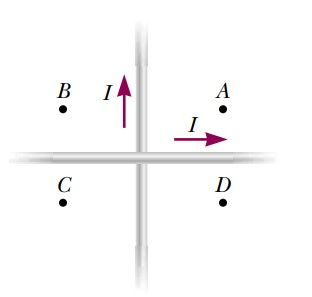
\includegraphics[width=0.3\linewidth]{figs/VN12-Y24-PH-SYL-017P-8}
	\end{center}
	\choice
	{vùng A và D}
	{\True vùng A và C}
	{vùng B và D}
	{vùng B và C}
	\loigiai{}
\end{ex}
% ===================================================================
\begin{ex}
	Xét dây dẫn có chiều dài $L$, có dòng điện $I$ chạy qua đặt tại điểm M trong từ trường đều, chịu tác dụng của lực điện từ $F$. Khi thay đổi $L$ hoặc $I$ thì $F$ thay đổi nhưng tỉ số nào sau đây luôn không đổi?
	\choice
	{$\frac{FI}{2L}$}
	{\True $\frac{F}{IL}$}
	{$\frac{FL}{I}$}
	{$\frac{FI^2}{L}$}
	\loigiai{}
\end{ex}
% ===================================================================
\begin{ex}
	Một đoạn dây dẫn đặt trong từ trường đều. Nếu chiều dài dây dẫn và cường độ dòng điện qua dây dẫn tăng 2 lần thì độ lớn lực từ tác dụng lên dây dẫn	
	\choice
	{tăng 2 lần}
	{giảm 2 lần}
	{\True tăng 4 lần}
	{không đổi}
	\loigiai{
		$$F=ILB\sin\theta.$$
	}
\end{ex}

% ===================================================================
\begin{ex}
	Một đoạn dây dẫn mang dòng điện được đặt vuông góc với từ trường đều có cảm ứng từ $B$. Khi dòng điện trong dây là $I$ thì lực từ tác dụng lên đoạn dây đó là $F$. Cũng đoạn dây đó, cho dòng điện chạy qua dây là $0,25I$ và đặt trong từ trường $2B$, lực từ tác dụng lên đoạn dây đó là
	\choice
	{$\dfrac{F}{4}$}
	{\True $\dfrac{F}{2}$}
	{$F$}
	{$2F$}
	\loigiai{}
\end{ex}
% ===================================================================
\begin{ex}
	Trong thí nghiệm đo độ lớn cảm ứng từ bằng "cân dòng điện" với bố trí thí nghiệm được thể hiện như trong hình \ref{fig:18P-11}, khung dây được sử dụng có kích thước là $\SI{100}{\milli\meter}\times\SI{80}{\milli\meter}$ như hình \ref{fig:18P-12}. Nếu ta thay khung dây ban đầu thành một khung dây khác có kích thước là $\SI{100}{\milli\meter}\times\SI{20}{\milli\meter}$ nhưng vẫn giữ nguyên góc hợp bởi mặt phẳng khung dây và các đường sức từ cũng như cường độ dòng điện qua khung dây và nam châm điện thì nhận định nào sau đây về lực từ do từ trường tác dụng lên khung dây là \textbf{đúng}?
	\begin{center}
		\begin{tabular}{M{8cm}M{8cm}}
			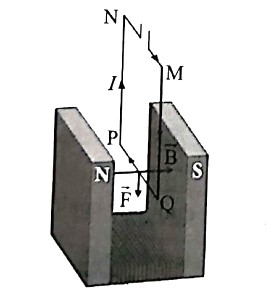
\includegraphics[width=0.6\linewidth]{figs/VN12-Y24-PH-SYL-018P-11}
			\captionof{figure}{}
			\label{fig:18P-11}
			&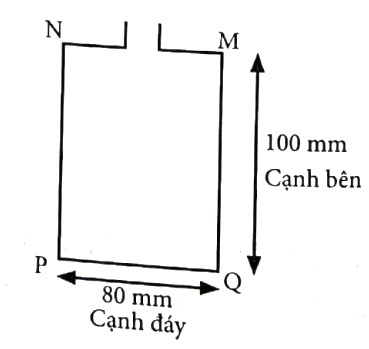
\includegraphics[width=0.6\linewidth]{figs/VN12-Y24-PH-SYL-018P-12}
			\captionof{figure}{}
			\label{fig:18P-12}
		\end{tabular}
	\end{center}
	\choice
	{Không đổi chiều và độ lớn tăng 4 lần}
	{\True Không đổi chiều và độ lớn giảm 4 lần}
	{Đổi chiều và độ lớn giảm 4 lần}
	{Đổi chiều và độ lớn tăng 4 lần}
	\loigiai{
		Vi từ trường chỉ tác dụng lực lên cạnh dưới của khung và độ lớn của lực từ được xác định bằng biểu thức $F=B I L$ nên khi chiều dài cạnh đáy giảm 4 lần thì độ lớn lực từ giảm 4 lần.
	}
\end{ex}


% ===================================================================
\begin{ex}
	Một đoạn dây dẫn dài $\ell=\SI{0.8}{\meter}$ đặt trong từ trường đều sao cho dây dẫn hợp với vector cảm ứng từ một góc $\SI{60}{\degree}$. Biết dòng điện $I=\SI{20}{\ampere}$ và dây dẫn chịu một lực là $F=\SI{2E-2}{\newton}$. Độ lớn của cảm ứng từ là
	\choice
	{$\SI{0.8E-3}{\tesla}$}
	{$\SI{E-3}{\tesla}$}
	{\True $\SI{1.4E-3}{\tesla}$}
	{$\SI{1.6E-3}{\tesla}$}
	\loigiai{
		$$B=\dfrac{F}{I\ell\sin\theta}=\dfrac{\SI{2E-2}{\newton}}{\left(\SI{20}{\ampere}\right)\cdot\left(\SI{0.8}{\meter}\right)\cdot\sin\SI{60}{\degree}}\approx\SI{1.44E-3}{\tesla}.$$
	}
\end{ex}

% ===================================================================
\begin{ex}
	Một đoạn dây dẫn dài $\SI{2}{\centi\meter}$ nằm trong từ trường, dòng điện chạy qua có cường độ $\SI{1}{\ampere}$. Một nam châm tạo từ trường có cường độ cảm ứng từ $\SI{0.5}{\tesla}$ và hợp với dây dẫn một góc $\SI{30}{\degree}$. Lực từ tác dụng lên dây dẫn có độ lớn là
	
	\choice
	{$\SI{10E-2}{\newton}$}
	{$\SI{1E-2}{\newton}$}
	{\True $\SI{0.5E-2}{\newton}$}
	{$\SI{50E-2}{\newton}$}
	\loigiai{
		$$
		F=BIL\sin \alpha=\SI{0.5E-2}{\newton}.
		$$
		
	}
\end{ex}
% ===================================================================
\begin{ex}
	Khi góc hợp bởi vector cảm ứng từ với đoạn dây dẫn có dòng điện là $\alpha=\SI{90}{\degree}$ thì lực từ tác dụng có giá trị là $\SI{0.4}{\newton}$. Nếu thay đổi góc $\alpha$ nhỏ dần đến $\SI{0}{\degree}$, thì lực tác dụng thay đổi như thế nào?
	\choice
	{\True Lực cũng giảm dần đến 0}
	{Lực tăng lên đến $\SI{0.8}{\newton}$}
	{Lực không đổi}
	{Lực giảm xuống $\SI{0.2}{\newton}$}
	\loigiai{}
\end{ex}

% ===================================================================
\begin{ex}
	Một dây dẫn thẳng có chiều dài $\SI{3.0}{\meter}$ mang dòng điện $\SI{6.0}{\ampere}$ được đặt nằm ngang, hướng của dòng điện tạo với hướng bắc một góc $\SI{50}{\degree}$ lệch về phía tây. Tại điểm này, cảm ứng từ của từ trường Trái Đất có độ lớn là $\SI{0.14E-4}{\tesla}$ và hướng bắc. Lực tác dụng lên dây có độ lớn là
	\choice
	{$\SI{0.28E-4}{\newton}$}
	{$\SI{2.5E-4}{\newton}$}
	{$\SI{1.9E-4}{\newton}$}
	{\True $\SI{1.6E-4}{\newton}$}
	\loigiai{
		$$F=ILB\sin\SI{50}{\degree}\approx\SI{1.6E-4}{\newton}.$$	
	}
\end{ex}
% ===================================================================
\begin{ex}
	Một dây đồng dài $\SI{25}{\centi\meter}$, có khối lượng là $\SI{10}{\gram}$ nằm trong từ trường $\SI{0.20}{\tesla}$. Lấy gia tốc trọng trường $g=\SI{10}{\meter/\second^2}$. Cường độ dòng điện nhỏ nhất chạy qua dây gây ra lực từ có độ lớn bằng trọng lượng của dây là
	\choice
	{$\SI{1.3}{\ampere}$}
	{$\SI{1.5}{\ampere}$}
	{\True $\SI{2.0}{\ampere}$}
	{$\SI{4.9}{\ampere}$}
	\loigiai{
		$$I_\text{min}=\dfrac{P}{BL\left(\sin\theta\right)_{\text{max}}}=\SI{2.0}{\ampere}.$$	
	}
\end{ex}
% ===================================================================
\begin{ex}
	Trong thí nghiệm xác định độ lớn cảm ứng từ của nam châm điện chữ $U$ bằng "cân dòng điện" (theo phương án thí nghiệm trong Bài 11 của SGK CTST), xét trạng thái ổn định với đòn cân nằm ngang cân bằng khi có dòng điện chạy trong khung dây và nam châm điện, góc hợp bởi mặt phẳng khung dây và các đường sức từ là $\SI{90}{\degree}$. Nếu ta làm khung dây bị lệch một góc nào đó so với vị trí ban đầu thì khi đòn cân được điều chỉnh trở về lại trạng thái nằm ngang cân bằng, số chỉ của lực kế sẽ	
	\choice
	{vẫn giữ nguyên giá trị ban đầu}
	{lớn hơn giá trị ban đầu}
	{\True nhỏ hơn giá trị ban đầu}
	{dao động xung quanh giá trị ban đầu}
	\loigiai{
		Vì độ lớn của lực từ được xác định bằng biểu thức $F=ILB\sin\theta$ nên khi khung dây bị lệch so với ban đầu thì $\sin\theta$ giảm dẫn đến $F$ giảm. Vì vậy số chỉ của lực kế giảm so với ban đầu.	
	}
\end{ex}


% ===================================================================
\begin{ex}
	Thanh dây dẫn thẳng MN có chiều dài $\SI{20}{\centi\meter}$, khối lượng $\SI{10}{\gram}$, được treo trên hai sợi dây mảnh sao cho MN nằm ngang. Cả hệ thống được đặt trong từ trường đều có cảm ứng từ $B=\SI{0.25}{\tesla}$ và vector $\vec{B}$ hướng lên trên theo phương thẳng đứng. Nếu cho dòng điện $I=\xsi{2\sqrt{3}}{\ampere}$ chạy qua, người ta thấy thanh MN được nâng lên vị trí cân bằng mới và hai sợi dây treo bây giờ lệch một góc $\alpha$ so với phương thẳng đứng. Cho $g=\SI{10}{\meter/\second^2}$, góc lệch $\alpha$ là	
	\begin{center}
		\begin{tikzpicture}
			\coordinate (A) at (0,0);
			\coordinate (B) at (3,1.5);
			\coordinate (A1) at ($(A)+(0,-1.5)$);
			\coordinate (B1) at ($(B)+(0,-1.5)$);
			\coordinate (M) at ($(A)+(-30:3)$);
			\coordinate (N) at ($(B)+(-30:3)$);
			\draw[line width=1pt] (A)--(M);
			\draw[line width=1pt] (B)--(N);
			\draw[line width=1pt, dashed] (A)--(A1);
			\draw[line width=1pt, dashed] (B)--(B1);
			\draw[line width=4pt] (M)--(N);
			\draw[line width=3pt, blue] (A)--+(30:0.5)--+(-150:0.5);
			\draw[line width=3pt, blue] (B)--+(30:0.5)--+(-150:0.5);
			\tkzMarkAngle[size=0.75cm,color=red](A1,A,M);
			\tkzLabelAngle[color=red,pos=1.2](A1,A,M){$\alpha$};
		\end{tikzpicture}
	\end{center}
	\choice
	{$\SI{30}{\degree}$}
	{$\SI{45}{\degree}$}
	{\True $\SI{60}{\degree}$}
	{$\SI{90}{\degree}$}
	\loigiai{}
\end{ex}

\Closesolutionfile{ans}

\subsubsection{Trắc nghiệm đúng/sai}
\Opensolutionfile{ans}[ans/VN12-Y24-PH-SYL-018P-TF]
\setcounter{ex}{0}
% ===================================================================
\begin{ex}
	Một thí nghiệm để tìm ra lực từ tác dụng lên một đoạn dây dẫn chứa dòng điện được đặt trong từ trường của một nam châm.
	\choiceTF[t]
	{\True Nếu cường độ dòng điện qua dây tăng lên, lực từ tác dụng lên dây sẽ tăng lên}
	{Nếu khoảng cách giữa dây dẫn và nam châm tăng lên, lực từ tác dụng lên dây sẽ tăng lên}
	{\True Lực từ chỉ có thể tác dụng lên dây dẫn khi có dòng điện chạy qua dây}
	{Độ lớn lực từ tác dụng lên đoạn dây dẫn sẽ thay đổi khi dòng điện chạy qua dây đảo chiều}
	\loigiai{}
\end{ex}
% ===================================================================
\begin{ex}
	Trong mỗi phát biểu sau, em hãy chọn đúng hoặc sai.	
	\choiceTF[t]
	{Cảm ứng từ là một đại lượng vô hướng}
	{\True Tiếp tuyến tại bất kì điểm nào trên đường sức từ đều có phương, chiều trùng với phương, chiều của vector cảm ứng từ tại điểm đó}
	{\True Từ trường ở vùng không gian giữa hai cực của nam châm chữ U được xem là từ trường đều}
	{Trong từ trường đều, các đường sức từ song song nhau nhưng vector cảm ứng từ tại các điểm khác nhau lại không bằng nhau về độ lớn}
	\loigiai{}
\end{ex}
% ===================================================================
\begin{ex}
	\immini{Xét một dây dẫn thẳng dài vô hạn có dòng điện cường độ $I$ chạy qua. Hai điểm M, N nằm trong cùng một mặt phẳng vuông góc với dây dẫn và cách đều dây dẫn, biết OM vuông góc với ON.\\
		Trong mỗi phát biểu sau về cảm ứng từ tại điểm M và N do dòng điện này gây ra, em hãy chọn đúng hoặc sai.	}
	{		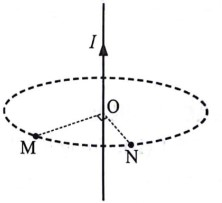
\includegraphics[width=0.4\linewidth]{figs/VN12-Y24-PH-SYL-018P-1}
	}
	
	\choiceTF[t]
	{\True Cảm ứng từ tại điểm M có phương vuông góc với OM}
	{cảm ứng từ tại điểm N song song với dây dẫn và có hướng cùng chiều với dòng điện chạy trong dây dẫn}
	{\True M và N cùng nằm trên một đường sức từ}
	{\True Cảm ứng từ tại M và N bằng nhau về độ lớn}
	\loigiai{}
\end{ex}

% ===================================================================
\begin{ex}
	Chỉ ra đáp án đúng, đáp án sai.
	\choiceTF[t]
	{\True Nam châm tác dụng lên dòng điện thực chất là tương tác giữa từ trường của nam châm với các electron của dây điện}
	{Nam châm tác dụng lên dòng điện thực chất là tương tác giữa từ trường của nam châm với từ trường do các electron chuyển động gây ra}
	{Phương của lực từ trùng với phương của dòng điện}
	{\True Lực từ tác dụng lên đoạn dây dẫn mang dòng điện có phương vuông góc với đoạn dây dẫn và vuông góc vector cảm ứng từ}
	\loigiai{}
\end{ex}
% ===================================================================
\begin{ex}
	Trong mỗi nhận định sau về thí nghiệm đo độ lớn cảm ứng từ bằng "cân dòng điện" với bố trí thí nghiệm được thể hiện như hình \ref{fig:18P-10}. Em hãy chọn đúng hoặc sai cho mỗi nhận định sau đây.
	\begin{center}
		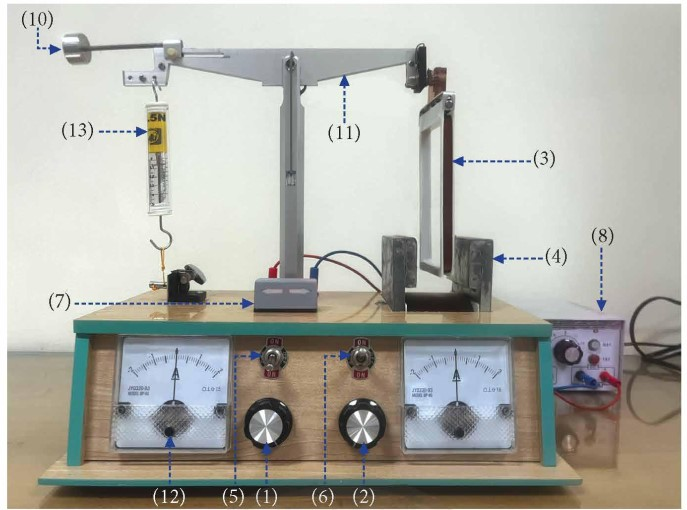
\includegraphics[width=0.55\linewidth]{figs/VN12-Y24-PH-SYL-018P-10}
		\captionof{figure}{Thí nghiệm đo độ lớn cảm ứng từ bằng "cân dòng điện"}
		\label{fig:18P-10}
	\end{center}
	\choiceTFt
	{\True Cơ sở lí thuyết của thí nghiệm này dựa trên tác dụng lực của từ trường đều lên đoạn dây dẫn có dòng điện chạy qua}
	{\True Trước khi bật công tắc cho dòng điện chạy qua khung dây dẫn và nam châm điện, cần phải điều chỉnh sao cho đòn cân nằm ngang rồi đọc giá trị của lực kế}
	{Khi đóng công tắc cho dòng điện chạy qua khung dây dẫn và nam châm điện, từ trường tạo ra bởi nam châm luôn tác dụng lực đẩy khung dây đi lên}
	{\True Trong thí nghiệm, từ trường tạo bởi nam châm điện không tác dụng lực từ lên các cạnh bên của khung dây}
	{Từ trường trong vùng không gian giữa hai nhánh của nam châm điện trong thí nghiệm được xem gần đúng là từ trường đều. Chiều và độ lớn của vector cảm ứng từ trong vùng từ trường này không phụ thuộc vào chiều và cường độ dòng điện chạy qua cuộn dây của nam châm}
	{Có thể lấy giá trị của lực kế khi đòn cân chưa nằm ngang ổn định}
	{\True Công dụng của các núm xoay (1) và (2) là điều chỉnh giá trị cường độ dòng điện chạy qua khung dây và cuộn dây của nam châm điện}
	{\True Có thể thay đổi chiều của lực từ tác dụng lên khung dây bằng việc sử dụng công tắc (5) hoặc (6)}
	\loigiai{}
\end{ex}

% ===================================================================
\begin{ex}
	Cho một khung dây dẫn hình chữ nhật có chiều rộng $\SI{20}{\centi\meter}$, mang dòng điện, đặt trong từ trường đều có cảm ứng từ $\vec{B}$ hướng vào trong như hình vẽ. Biết mặt phẳng vòng dây vuông góc với các đường sức từ. Bên ngoài vòng tròn, từ trường bằng 0.\begin{center}
		\begin{tikzpicture}
			\foreach \x in {-3,-2,...,3}{
				\foreach \y in {-3,-2,...,3}{
					\node[blue] at (\x,\y) {\LARGE$\odot$};
					
			}}
			\fill[white, even odd rule] (0,0) circle(3.4) (0,0) circle (4.5);
			\draw[dashed, line width=1pt] (0,0) circle (3.5);
			\draw[line width=1.5pt,decoration={markings, mark=at position 0.5 with {\arrow{stealth}}},postaction={decorate}
			] (-1.5,3.75)--(-1.5,0.65)--(1.5,0.65)--(1.5,3.75);
			\node[black] at (0,0.35) {$\SI{20}{\centi\meter}$};
		\end{tikzpicture}
	\end{center}
	\choiceTF[t]
	{\True Lực từ tổng hợp tác dụng lên khung dây hướng xuống dưới}
	{Nếu sử dụng dòng điện có cường độ $\SI{5.00}{\ampere}$ thì lực từ trên mỗi tesla tác dụng lên khung dây là $\SI{2.00}{\newton/\tesla}$}
	{\True Nếu ta quay khung dây $\SI{90}{\degree}$ xung quanh một trục nằm trong mặt phẳng của khung và song song với từ trường, lực từ tác dụng lên khung sẽ giảm xuống bằng 0}
	{\True Khi dòng điện qua khung dây đổi chiều, lực từ tổng hợp tác dụng lên khung dây sẽ đổi chiều}
	\loigiai{
		\begin{itemchoice}
			\itemch Đúng. Vì lực từ tổng hợp tác dụng lên hai đoạn dây thẳng đứng bị triệt tiêu, chỉ còn lực tác dụng lên đoạn dây dẫn nằm ngang và lực này hướng xuống dưới.
			\itemch Sai. Vì $\dfrac{F}{B}=IL\sin\SI{90}{\degree}=\SI{1}{\newton/\tesla}$.
			\itemch Đúng. Lực từ tổng hợp tác dụng lên hai dây dẫn thẳng đứng bị triệt tiêu, còn dây nằm ngang song song với từ trường nên lực từ tác dụng lên nó bằng 0.
			\itemch Đúng. Hướng lực từ phụ thuộc vào hướng của dòng điện theo quy tắc bàn tay trái.
			
		\end{itemchoice}	
	}
\end{ex}
% ===================================================================
\begin{ex}
	Một đoạn dây thẳng bằng đồng được đặt vuông góc với từ trường đều, có dòng điện $\SI{7.0}{\ampere}$ chạy qua và nằm cân bằng trong từ trường. Khối lượng của một đơn vị chiều dài của đoạn dây là $\SI{46.6}{\gram/\meter}$, và gia tốc trọng trường là $\SI{9.8}{\meter/\second^2}$. Bỏ qua ảnh hường của từ trường Trái Đất lên đoạn dây.
	\begin{center}
		\begin{tikzpicture}
			\node[blue] at (0,0) {\LARGE$\odot$};
			\node[left] at (-0.25,0) {$I$};
			\draw[-latex, line width=1.5pt] (0,0)--+(0,-1.5);
			\node[left] at (0,-1.5) {$\vec{P}$};
		\end{tikzpicture}
	\end{center}
	\choiceTF[t]
	{\True Lực từ tác dụng lên đoạn dây sẽ tăng lên nếu cảm ứng từ trong từ trường đều tăng lên mà dòng điện giữ nguyên}
	{Cảm ứng từ $\vec{B}$ có phương nằm ngang và chiều từ phải sang trái}
	{\True Lực từ có thể cân bằng với trọng lực khi đoạn dây được đặt trong một từ trường với cảm ứng từ bằng $\SI{6.5E-2}{\tesla}$}
	{Nếu thay dây dẫn trên bằng dây dẫn nhôm có cùng kích cỡ nhưng khối lượng riêng thấp hơn, thì lực từ cần để cân bằng dây sẽ tăng}
	\loigiai{
		\begin{itemchoice}
			\itemch Đúng. Vì $F=ILB\sin\theta$.
			\itemch Sai. Áp dụng quy tắc bàn tay trái, cảm ứng từ có phương nằm ngang và chiều từ trái sang phải.
			\itemch Đúng. Khối lượng dây $m=\SI{46.6E-3}{}\cdot\ell$.\\
			Lực từ và trọng lực có thể cân bằng nhau nếu cảm ứng từ $B$ được điều chỉnh sao cho
			$$F=P\Leftrightarrow mg=I\ell B\Rightarrow B=\dfrac{m}{\ell}\cdot\dfrac{g}{I}=\SI{6.5E-2}{\tesla}.$$
			\itemch Sai. Nếu khối lượng riêng giảm thì trọng lực sẽ giảm, nên lực từ giảm để cân bằng.
		\end{itemchoice}	
	}
\end{ex}
% ===================================================================
\begin{ex}
	Trong giờ thực hành đo độ lớn cảm ứng từ bằng "cân dòng điện" với bố trí thí nghiệm được thể hiện như trong hình \ref{fig:18P-10}, một bạn học sinh thu được bảng số liệu như bảng dưới đây.
	\begin{center}
		\begin{tabular}{|M{2cm}|M{2cm}|M{2cm}|M{2cm}|M{4cm}|M{3.5cm}|}
			\hline
			\multicolumn{6}{|M{17cm}|}{$\theta=\SI{90}{\degree}$; $L=\SI{0.08}{\meter}$; $N=\SI{200}{\text{vòng}}$}\\
			\hline
			\thead{Lần đo} & $\xsi{I}{\left(\ampere\right)}$ & $\xsi{F_1}{\left(\newton\right)}$ & $\xsi{F_2}{\left(\newton\right)}$ & $F=\xsi{F_2-F_1}{\left(\newton\right)}$ & $B=\xsi{\frac{F}{NIL}}{\left(\tesla\right)}$\\
			\hline
			1 & 0,2 & 0,210 & 0,270 &&\\
			\hline
			2 & 0,4 & 0,210 & 0,320 & &\\
			\hline
			3 & 0,6 & 0,210 & 0,380 & &\\
			\hline
			\multicolumn{5}{|M{12cm}|}{\thead{Trung bình}} &$\overline{B}=$\\
			\hline
			
		\end{tabular}
	\end{center}
	Biết rằng giới hạn đo và độ chia nhỏ nhất của các ampe kế lần lượt là $\SI{2.0}{\ampere}$ và $\SI{0.1}{\ampere}$. Trong mỗi phát biểu sau, em hãy chọn đúng hoặc sai.
	\choiceTF[t]
	{\True Giá trị độ lớn cảm ứng từ thu được ở các lần đo có sự khác nhau là do có sai số trong quá trình đo đạc, thu thập và xử lí số liệu}
	{Giá trị trung bình của độ lớn cảm ứng từ thu được trong thí nghiệm này là $\SI{0.015}{\tesla}$ (làm tròn đến 3 chữ số thập phân sau dấu phẩy)}
	{Trong quá trình điều chỉnh dòng điện, giá trị của cường độ dòng điện đọc được từ ampe kế có thể bằng $\SI{0.25}{\ampere}$}
	{Sai số tuyệt đối trung bình của độ lớn cảm ứng từ xấp xỉ $\SI{0.0001}{\tesla}$ (làm tròn đến 4 chữ số thập phân sau dấu phấy)}
	\loigiai{
		\begin{center}
			\begin{tabular}{|M{2cm}|M{2cm}|M{2cm}|M{2cm}|M{4cm}|M{3.5cm}|}
				\hline
				\multicolumn{6}{|M{17cm}|}{$\theta=\SI{90}{\degree}$; $L=\SI{0.08}{\meter}$; $N=\SI{200}{\text{vòng}}$}\\
				\hline
				\thead{Lần đo} & $\xsi{I}{\left(\ampere\right)}$ & $\xsi{F_1}{\left(\newton\right)}$ & $\xsi{F_2}{\left(\newton\right)}$ & $F=\xsi{F_2-F_1}{\left(\newton\right)}$ & $B=\xsi{\frac{F}{NIL}}{\left(\tesla\right)}$\\
				\hline
				1 & 0,2 & 0,210 & 0,270 &0,060&0,019\\
				\hline
				2 & 0,4 & 0,210 & 0,320 &0,110 &0,017\\
				\hline
				3 & 0,6 & 0,210 & 0,380 &0,170 &0,018\\
				\hline
				\multicolumn{5}{|M{12cm}|}{\thead{Trung bình}} &$\overline{B}=0,0180$\\
				\hline
				
			\end{tabular}
		\end{center}	
		Sai số trung bình:
		$$\begin{aligned}
			\Delta \overline{B}&=\dfrac{\left|\overline{B}-B_1\right|+\left|\overline{B}-B_2\right|+\left|\overline{B}-B_3\right|}{3}\\
			&=\dfrac{\left|0,0180-0,0190\right|+\left|0,0180-0,017\right|+\left|0,0180-0,0180\right|}{3}\approx\SI{0.0007}{\tesla}.
		\end{aligned}$$
		
	}
\end{ex}



\Closesolutionfile{ans}
\subsubsection{Tự luận}
\setcounter{ex}{0}
\Opensolutionfile{ans}[ans/VN12-Y24-PH-SYL-018P-TL]
% ===================================================================
\begin{ex}
	Thanh kim loại dẫn điện có thể lăn không ma sát dọc theo hai đoạn dây dẫn không nhiễm từ. Khi đóng công tắc K, dòng điện chạy theo chiều mũi tên.
	\begin{center}
		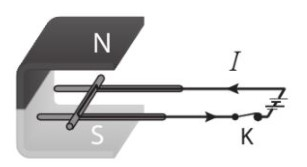
\includegraphics[width=0.3\linewidth]{figs/VN12-Y24-PH-SYL-018P-8}
	\end{center}
	\begin{enumerate}[label=\alph*)]
		\item Thanh kim loại sẽ lăn theo hướng nào khi đóng công tắc K?
		\item Nêu cách làm cho thanh kim loại lăn theo hướng ngược lại.
	\end{enumerate}
	\loigiai{
		\begin{enumerate}[label=\alph*)]
			\item Thanh kim loại dẫn điện sẽ lăn về bên phải.
			\item Đảo ngược chiều dòng điện hoặc đổi chiều của từ trường.
		\end{enumerate}	
	}
\end{ex}

% ===================================================================
\begin{ex}
	Xác định hướng của lực từ tác dụng lên các đoạn dây dẫn có dòng điện chạy qua, được đặt trong từ trường đều như các hình dưới đây:
	\begin{center}
		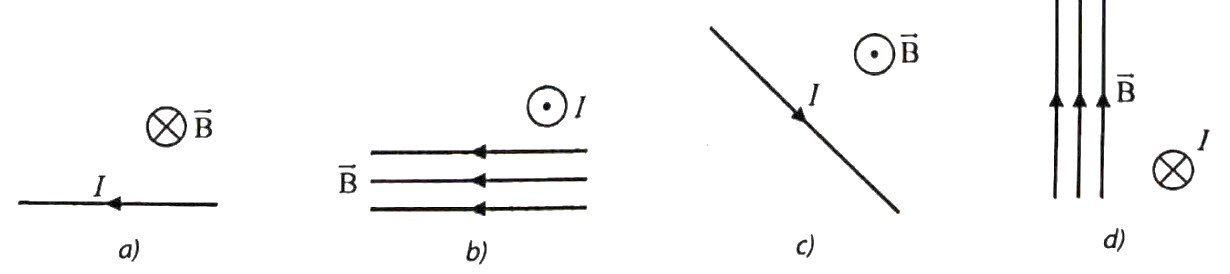
\includegraphics[width=0.8\linewidth]{figs/VN12-Y24-PH-SYL-018P-3}
	\end{center}
	\loigiai{
		\begin{center}
			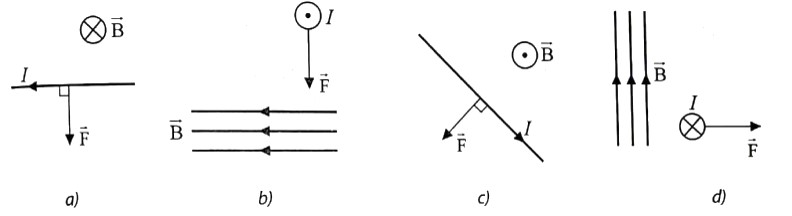
\includegraphics[width=0.8\linewidth]{figs/VN12-Y24-PH-SYL-018P-4}
		\end{center}	
	}
\end{ex}
% ======================================================================
\begin{ex}
	Xác định phương và chiều lực từ tác dụng lên các cạnh của khung. Biết chiều của vector cảm ứng từ $\vec{B}$ và chiều dòng điện được cho như mỗi hình vẽ.
	\begin{center}
		\begin{tabular}{cc}
			\begin{tikzpicture}
				\coordinate (A) at(0,0);
				\coordinate (B) at(0,-3);
				\coordinate (C) at(4,-3);
				\coordinate (D) at(0.5,0);
				\draw[decoration={markings, mark=at position 0.5 with{\arrow{stealth}}}, postaction={decorate}, line width=1.5pt](A)--(B)--(C)--(D);
				\foreach \y in {-0.5,-1.5,-2.5}{
					\draw[-latex, blue, line width=1.5pt] (-1,\y) --(4.5,\y);	
					\node[blue] at(4.5,0) {$\vec{B}$};
				}
				\node[left] at(A) {A};
				\node[left] at(B) {B};
				\node[right] at(C) {C};
				\node[above right] at(D) {D};
			\end{tikzpicture}
			&
			\begin{tikzpicture}
				\coordinate (A) at(0,0);
				\coordinate (B) at(0,-3);
				\coordinate (C) at(4,-3);
				\coordinate (D) at(4,0);
				\coordinate (E) at(0.5,0);
				\draw[decoration={markings, mark=at position 0.35 with{\arrow{stealth}}}, postaction={decorate}, line width=1.5pt](A)--(B)--(C)--(D)--(E);
				
				\node[left] at(A) {A};
				\node[left] at(B) {B};
				\node[right] at(C) {C};
				\node[right] at(D) {D};
				\node[above] at(E) {E};
				\node[blue] at(2,-1.5) {\LARGE $\odot$};
				\node[blue, right] at(2.2,-1.5) {$\vec{B}$};
			\end{tikzpicture}\\
			Hình a & Hình b
		\end{tabular}
	\end{center}
	\loigiai{
		\begin{center}
			\begin{tabular}{M{6cm}M{6cm}}
				\begin{tikzpicture}
					\coordinate (A) at(0,0);
					\coordinate (B) at(0,-3);
					\coordinate (C) at(4,-3);
					\coordinate (D) at(0.5,0);
					\draw[decoration={markings, mark=at position 0.5 with{\arrow{stealth}}}, postaction={decorate}, line width=1.5pt](A)--(B)--(C)--(D);
					\foreach \y in {-0.5,-1.5,-2.5}{
						\draw[-latex, blue, line width=1.5pt] (-1,\y) --(4.5,\y);	
						\node[blue] at(4.5,0) {$\vec{B}$};
					}
					\node[left] at(A) {A};
					\node[left] at(B) {B};
					\node[right] at(C) {C};
					\node[above right] at(D) {D};
					\node[red, fill=white, minimum size=0pt,inner sep=0pt, circle] at (0,-1.5) {\LARGE$\odot$};
					\node[red, below right] at (0.25,-1.5) {$\vec{F}_{\text{AB}}$};
					\node[red, fill=white, minimum size=0pt,inner sep=0pt, circle] at ($(D)!0.5!(C)$) {\LARGE$\otimes$};
					\node[red, below] at ($(D)!0.5!(C)+(0,-0.25)$) {$\vec{F}_{\text{CD}}$};
				\end{tikzpicture}
				&
				\begin{tikzpicture}
					\coordinate (A) at(0,0);
					\coordinate (B) at(0,-3);
					\coordinate (C) at(4,-3);
					\coordinate (D) at(4,0);
					\coordinate (E) at(0.5,0);
					\draw[decoration={markings, mark=at position 0.35 with{\arrow{stealth}}}, postaction={decorate}, line width=1.5pt](A)--(B)--(C)--(D)--(E);
					\draw[-latex, red, line width=1.5pt] ($(A)!0.5!(B)$)--+(-1,0);
					\draw[-latex, red, line width=1.5pt] ($(B)!0.5!(C)$)--+(0,-1);
					\draw[-latex, red, line width=1.5pt] ($(C)!0.5!(D)$)--+(1,0);
					\draw[-latex, red, line width=1.5pt] ($(D)!0.5!(E)$)--+(0,1);
					\node[left] at(A) {A};
					\node[left] at(B) {B};
					\node[right] at(C) {C};
					\node[right] at(D) {D};
					\node[above] at(E) {E};
					\node[blue] at(2,-1.5) {\LARGE $\odot$};
					\node[blue, right] at(2.2,-1.5) {$\vec{B}$};
					\node[red, above] at ($(A)!0.5!(B)+(-1,0)$) {$\vec{F}_{\text{AB}}$};
					\node[red, right] at ($(B)!0.5!(C)+(0,-1)$) {$\vec{F}_{\text{BC}}$};
					\node[red, above] at ($(C)!0.5!(D)+(1,0)$) {$\vec{F}_{\text{CD}}$};
					\node[red, right] at ($(D)!0.5!(E)+(0,1)$) {$\vec{F}_{\text{DE}}$};
				\end{tikzpicture}\\
				Hình a & Hình b
			\end{tabular}
		\end{center}	
	}
\end{ex}



% ===================================================================
\begin{ex}
	\immini{Động cơ điện là thiết bị có thể chuyển hoá năng lượng điện thành cơ năng (chuyển động quay của động cơ). Mô hình đơn giản của một động cơ điện gồm: một khung dây dẫn hình chữ nhật ABCD đang có dòng điện không đổi chạy qua. Khung dây được đặt vào trong từ trường đều có các đường sức từ thẳng đứng như hình bên. Tại thời điểm ban đầu, khung đang ở vị trí sao cho hai cạnh AB và CD đang song song với các đường sức từ. Vẽ các lực từ tác dụng lên các cạnh của khung dây. Các lực này có tác dụng làm cho khung dây chuyển động như thế nào?	}
	{
		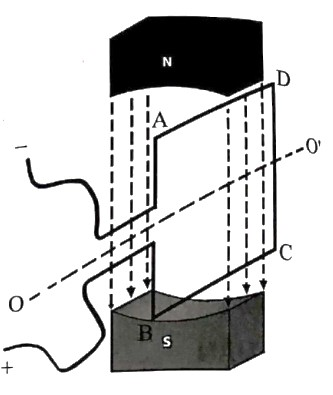
\includegraphics[width=0.45\linewidth]{figs/VN12-Y24-PH-SYL-018P-5}
	}
	\loigiai{
		Chỉ có lực từ tác dụng lên hai cạnh AD và BC của khung dây. Hai lực này tạo ra cặp ngẫu lực và có tác dụng tạo ra moment ngẫu lực làm quay khung dây.
		\begin{center}
			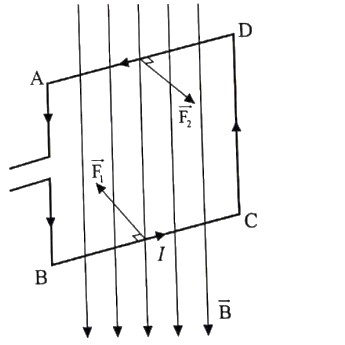
\includegraphics[width=0.4\linewidth]{figs/VN12-Y24-PH-SYL-018P-6}
		\end{center}	
	}
\end{ex}

% =================================================================
\begin{ex}
	Cho hai dây dẫn thẳng song song, dài vô hạn lần lượt có dòng điện $I_1$ và $I_2$ chạy qua như hình \ref{fig:17P-1}. Xét mặt phẳng $\left(Oxy\right)$ vuông góc với cả hai dòng điện, cắt các dòng điện tại A và B.
	\begin{center}
		\begin{tikzpicture}
			\coordinate (O) at (0,0);
			\coordinate (A) at ($(O)+(75:3)$);
			\coordinate (C) at (6,0);
			\coordinate (B) at ($(C)+(75:3)$);
			\fill[orange!50!white, opacity=0.6] (O)--(A)--(B)--(C)--(O);
			\draw[-latex, line width=1.5pt] (O)--+(75:4);
			\draw[-latex, line width=1.5pt] (O)--+(7,0);
			\draw[line width=1pt, dashed] (1,1.45)--(6,1.45);
			\draw[line width=1.5pt, blue,decoration={markings, mark=at position 0.625 with {\arrow{stealth}}},
			postaction={decorate}] 
			(1.5,1.45)--+(0,2.5);
			\draw[line width=1.5pt, blue, dashed] (1.5,1.45)--+(0,-1.45);
			\draw[line width=1.5pt, blue] (1.5,0)--+(0,-1);
			\draw[line width=1.5pt, blue,decoration={markings, mark=at position 0.625 with {\arrow{stealth}}},
			postaction={decorate}] 
			(3.5,1.45)--+(0,2.5);
			\draw[line width=1.5pt, blue, dashed] (3.5,1.45)--+(0,-1.45);
			\draw[line width=1.5pt, blue] (3.5,0)--+(0,-1);
			\filldraw (1.5,1.45) circle(2pt) node[above left] {A};
			\filldraw (3.5,1.45) circle(2pt) node[above left] {B};
			\filldraw (5,1.45) circle(2pt) node[above left] {C};
			\node[left] at (O) {O};
			\node[below] at (7,0) {$x$};
			\node[left] at ($(O)+(75:4)$) {$y$};
			\node[right] at (1.5,3) {$I_1$};
			\node[right] at (3.5,3) {$I_2$};
		\end{tikzpicture}
	\end{center}
	\captionof{figure}{}
	\label{fig:17P-1}
	\begin{enumerate}[label=\alph*)]
		\item Xác định phương, chiều của các vector cảm ứng từ do từng dòng điện gây ra tại C (A, B, C thẳng hàng).
		\item Nếu đặt một kim la bàn tại điểm C thì kim la bàn này sẽ định hướng như thế nào? Giải thích.
	\end{enumerate}
	\loigiai{\begin{enumerate}[label=\alph*)]
			\item Dựa vào quy tắc nắm tay phải, ta xác định được vector cảm ứng từ do hai dòng điện $I_1$ và $I_2$ gây ra tại điểm C đều nằm trong mặt phẳng $\left(Oxy\right)$, phương song song và cùng chiều với trục $Oy$.
			\item Hai vector cảm ứng từ do hai dòng điện $I_1$ và $I_2$ gây ra đều cùng hướng với nhau nên kim la bàn khi đặt tại C sẽ có cực Bắc hướng theo chiều dương trục $Oy$ còn cực Nam hướng ngược lại.
	\end{enumerate}}
\end{ex}
% ===================================================================
\begin{ex}
	Một dây dẫn có chiều dài $L=\SI{1.2}{\meter}$, được đặt trong từ trường đều có độ lớn $B=\SI{5E-2}{\tesla}$. Cường độ dòng điện chạy trong dây dẫn có giá trị $\SI{3}{\ampere}$. Hãy xác định độ lớn của lực từ tác dụng lên dây dẫn trong các trường hợp sau đây:
	\begin{enumerate}[label=\alph*)]
		\item Dây dẫn đặt vuông góc với các đường sức từ.
		\item Dây dẫn đặt song song với các đường sức từ.
		\item Dây dẫn hợp với các đường sức từ một góc $\SI{45}{\degree}$.
	\end{enumerate}	
	\loigiai{
		\begin{enumerate}[label=\alph*)]
			\item $F=ILB\sin\SI{90}{\degree}=\SI{0.18}{\newton}$.
			\item $F=ILB\sin\SI{0}{\degree}=\SI{0}{\newton}$.
			\item $F=ILB\sin\SI{45}{\degree}\approx\SI{0.13}{\newton}$.
		\end{enumerate}	
	}
\end{ex}
% ===================================================================
\begin{ex}
	Một đoạn dây dẫn thẳng dài $\SI{20}{\centi\meter}$ mang dòng điện có cường độ $\SI{50}{\milli\ampere}$ được đặt vào một vùng từ trường đều có cảm ứng từ $\SI{100}{\micro\tesla}$. Xác định góc hợp bởi đoạn dây và vector cảm ứng từ để lực từ tác dụng lên đoạn dây đạt độ lớn cực đại. Tính giá trị cực đại này.	
	\loigiai{
		Từ biểu thức tính độ lớn lực từ $F=B I L \sin \theta$, ta thấy lực từ đạt độ lớn cực đại khi: $\sin \theta=1 \Rightarrow \theta=\SI{90}{\degree}$. Khi đó, $F=B I L=100 \cdot 10^{-6} \cdot 50 \cdot 10^{-3} \cdot 0,2=\SI{E-6}{\newton}$.
		
	}
\end{ex}

% ===================================================================
\begin{ex}
	Một đoạn dây dẫn dài $\SI{5}{\centi\meter}$ đặt trong từ trường đều và vuông góc với vector cảm ứng từ. Dòng điện chạy qua dây có cường độ $\SI{0.75}{\ampere}$. Lực từ tác dụng lên đoạn dây đó là $\SI{3E-2}{\newton}$. Tính độ lớn cảm ứng từ.
	\loigiai{
		$$
		B=\frac{F}{IL\sin \theta}=\frac{3 \cdot 10^{-2}}{0,75 \cdot 0,05 \cdot \sin \SI{90}{\degree}}=\SI{0.8}{\tesla}.
		$$	
	}
\end{ex}
% ===================================================================
\begin{ex}
	Một đoạn dây dẫn dài $\SI{10}{\centi\meter}$ đặt trong từ trường đều, hợp với vector cảm ứng từ một góc $\SI{30}{\degree}$. Dòng điện có cường độ $\SI{2}{\ampere}$ chạy qua dây dẫn thì lực từ tác dụng lên đoạn dây có độ lớn là $\SI{4E-2}{\newton}$. Tính độ lớn của cảm ứng từ.
	\loigiai{
		Ta có: $\alpha=\SI{30}{\degree} \Rightarrow \sin \theta=\frac{1}{2}$. \\
		Cảm ứng từ của từ trường có độ lớn: $B=\dfrac{F}{IL\sin \theta}=\dfrac{4 \cdot 10^{-3}}{2 \cdot 0,1 \cdot 0,5}=\SI{0.04}{\tesla}$.	
	}
\end{ex}
% ===================================================================
\begin{ex}
	Một đoạn dây dẫn thẳng MN có chiều dài $\SI{6}{\centi\meter}$, có cường độ dòng điện $I=\SI{5}{\ampere}$ chạy qua đặt trong từ trường đều có cảm ứng từ $B=\SI{0.5}{\tesla}$. Lực từ tác dụng lên đoạn dây có độ lớn $F=\SI{7.5E-2}{\newton}$. Tính góc $\theta$ hợp bởi dây MN và vector cảm ứng từ.	
	\loigiai{
		Độ lớn của lực từ tác dụng lên đoạn dây dẫn có chiều dài $L$ mang dòng điện $I$ đặt trong từ trường cảm ứng từ $B$ là: $F=ILB \sin\theta \Rightarrow \sin\theta=0,5 \Rightarrow \theta=\SI{30}{\degree}.$	
	}
\end{ex}
% ===================================================================
\begin{ex}
	Một đoạn dây dài $L$ đặt trong từ trường đều có cảm ứng từ $B=\SI{0.5}{\tesla}$ hợp với đường cảm ứng từ một góc $\SI{30}{\degree}$. Dòng điện qua dây có cường độ $\SI{0.5}{\ampere}$, thì lực từ tác dụng lên đoạn dây là $\SI{4E-2}{\newton}$. Tính chiều dài đoạn dây dẫn.	
	\loigiai{
		Chiều dài đoạn dây dẫn:
		$$
		L=\frac{F}{IB \sin \theta}=\frac{4 \cdot 10^{-2}}{0,5 \cdot 0,5 \cdot \sin \SI{30}{\degree}}=\SI{0.32}{\meter}=\SI{32}{\centi\meter}.
		$$
		
	}
\end{ex}
% ===================================================================
\begin{ex}
	Một đoạn dây dẫn dài $L=\SI{0.5}{\meter}$ đặt trong từ trường đều sao cho dây dẫn hợp với vector cảm ứng từ một góc $\SI{45}{\degree}$. Biết cảm ứng từ $B=\SI{0.2}{\tesla}$ và dây dẫn chịu lực từ $F=\SI{4E-2}{\newton}$. Tính cường độ dòng điện chạy qua dây dẫn.
	\loigiai{
		$$
		I=\frac{F}{BL \sin \theta}=\frac{4 \cdot 10^{-2}}{0,2 \cdot 0,5 \cdot \sin \SI{45}{\degree}}=\xsi{0,4\sqrt{2}}{\ampere}.
		$$
		
	}
\end{ex}
% ===================================================================
\begin{ex}
	Một đường dây tải điện thẳng dài $\SI{42}{\meter}$ có dòng điện với cường độ $\SI{150}{\ampere}$ chạy qua theo hướng về phía Bắc. Từ trường Trái Đất tại vị trí này có độ lớn khoảng $\SI{0.5E-4}{\tesla}$, có hướng lệch một góc $\theta=\SI{50}{\degree}$ so với dòng điện. Xác định lực từ tác dụng lên đường dây nói trên.
	\begin{center}
		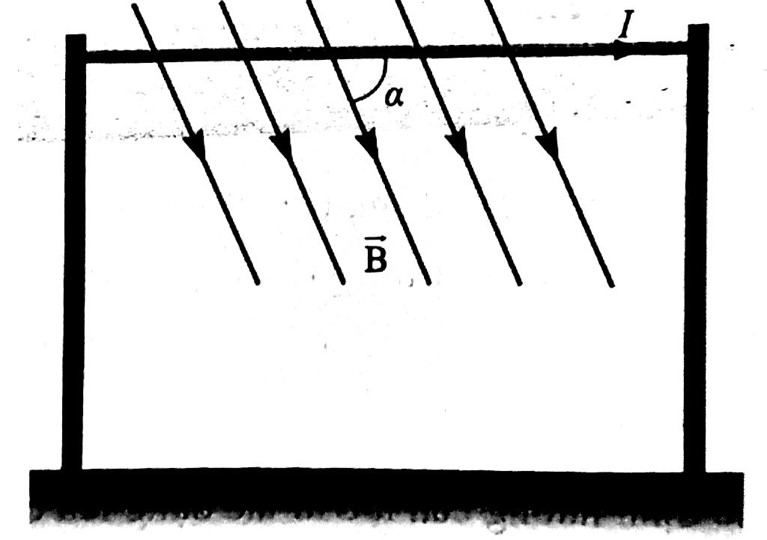
\includegraphics[width=0.4\linewidth]{figs/VN12-Y24-PH-SYL-018P-7}
	\end{center}
	\loigiai{
		Lực từ tác dụng lên đường dây có chiều hướng về phía Tây và có độ lớn là:
		$$F=B I L \sin \theta=0,5 \cdot 10^{-4} \cdot 150 \cdot 42 \cdot \sin \SI{50}{\degree} \approx \SI{0.24}{\newton}.$$
		
	}
\end{ex}
% ======================================================================
\begin{ex}
	Một dây dẫn có dòng điện $\SI{22.0}{\ampere}$ chạy từ Tây sang Đông. Giả sử tại vị trí này, từ trường Trái Đất nằm ngang và hướng từ Nam lên Bắc với độ lớn $\SI{0.5E-4}{\tesla}$.
	\begin{enumerate}[label=\alph*)]
		\item Tìm độ lớn và hướng của lực từ tác dụng lên một đoạn dây dài $\SI{36.0}{\meter}$.
		\item Tính lực hấp dẫn tác dụng lên đoạn dây có cùng chiều dài nếu nó được làm bằng đồng và có diện tích mặt cắt ngang là $\SI{2.50E-6}{\meter^2}$. Khối lượng riêng của đồng là $\SI{8.9E3}{\kilogram/\meter^3}$, lấy $g=\SI{9.80}{\meter/\second^2}$.
	\end{enumerate}
	\loigiai{
		\begin{enumerate}[label=\alph*)]
			\item $F_{\text{từ}}=ILB=\SI{3.96E-2}{\newton}$, hướng vuông góc với trang giấy, từ sau ra trước.
			\item $F_{\text{hấp dẫn}}=\rho gLS=\SI{7.85}{\newton}$.
			
		\end{enumerate}	
	}
\end{ex}
% ======================================================================
\begin{ex}
	Một dây dẫn thẳng, cứng, dài $\SI{20}{\centi\meter}$, có khối lượng $\SI{50}{\gram}$ được giữ nằm yên theo phương ngang trong một từ trường có độ lớn cảm ứng từ là $\SI{0.49}{\tesla}$ và có hướng nằm ngang, vuông góc với dây. Cường độ dòng điện chạy trong dây là bao nhiêu để khi dây được thả ra thì nó vẫn nằm yên? Lấy $g=\SI{9.8}{\meter/\second^2}$.
	
	\loigiai{
		$$F_{\text{từ}}	=P\Leftrightarrow ILB=mg\Rightarrow I=\dfrac{mg}{BL}=\SI{5.0}{\ampere}.$$
	}
\end{ex}

% ===================================================================
\begin{ex}
	Treo một đoạn dây dẫn có chiều dài $L=\SI{5}{\centi\meter}$, khối lượng $m=\SI{5}{\gram}$ bằng hai dây mảnh, nhẹ sao cho dây dẫn nằm ngang. Biết cảm ứng từ của từ trường hướng thẳng đứng xuống dưới, có độ lớn $B=\SI{0.5}{\tesla}$ và dòng điện chạy qua dây dẫn là $I=\SI{2}{\ampere}$. Lấy $g=\SI{10}{\meter/\second^2}$. Tính góc lệch của dây treo so với phương thẳng đứng.
	\loigiai{
		$$
		\tan \theta=\frac{F_t}{P}=\frac{0,5 \cdot 2 \cdot 0,05}{0,005 \cdot 10}=1 \Rightarrow \theta=\SI{45}{\degree}.
		$$
		
	}
\end{ex}
% ===================================================================
\begin{ex}
	Một đoạn dây dẫn thẳng MN có chiều dài $L=\SI{6}{\centi\meter}$, có dòng điện cường độ $I=\SI{5}{\ampere}$ chạy qua đặt trong từ trường đều có cảm ứng từ $B=\SI{0.5}{\tesla}$. Lực từ tác dụng lên đoạn dây có độ lớn $F=\SI{7.5E-2}{\newton}$. Tính góc $\theta$ hợp bởi dây MN và vector cảm ứng từ.
	\loigiai{
		Áp dụng công thức $F=ILB \sin \theta$ với $L=\SI{6E-2}{\meter}, I=\SI{5}{\ampere}, F=\SI{7.5E-2}{\newton}$ và $B=\SI{0.5}{\tesla}$, ta tính được $\theta=\SI{30}{\degree}$.
		
	}
\end{ex}
% ======================================================================
\begin{ex}
	Thanh MN dài $\ell=\SI{20}{\centi\meter}$ có khối lượng $\SI{5}{\gram}$ treo nằm ngang bằng hai sợi chỉ mảnh CM và DN. Thanh nằm trong từ trường đều có cảm ứng từ	 $B=\SI{0.3}{\tesla}$ nằm ngang vuông góc với thanh có chiều như hình vẽ. Mỗi sợi chỉ treo thanh có thể chịu được lực kéo tối đa là $\SI{0.04}{\newton}$. Dòng điện chạy qua thanh MN có chiều và cường độ lớn nhất là bao nhiêu thì sợi chỉ treo thanh chưa bị đứt. Lấy gia tốc trọng trường $g=\SI{9.8}{\meter/\second^2}$.
	\begin{center}
		\begin{tikzpicture}
			\coordinate (C) at (0,0);
			\coordinate (D) at (4,0);
			\coordinate (M) at (0,-3);
			\coordinate (N) at (4,-3);
			\draw[line width=1pt] (C)--+(-0.5,0)--+(4.5,0);
			\draw[line width=1pt] (C)--(M);
			\draw[line width=1pt] (D)--(N);
			\draw[line width=3pt] (M)--(N);
			\node[blue] at (2,-1.5) {\LARGE$\otimes$};
			\node[blue, right] at (2.25,-1.5) {$\vec{B}$};
			\node[above] at (C) {C};
			\node[above] at (D) {D};
			\node[left] at (M) {M};
			\node[right] at (N) {N};
		\end{tikzpicture}
	\end{center}
	\loigiai{
		Khi cho dòng điện chạy qua dây dẫn đặt trong từ trường thì sẽ có lực từ tác dụng lên dây dẫn.
		\begin{itemize}
			\item Công thức tính lực từ: $F=IB \ell \sin \alpha$.
			\item Dây bị đứt khi lực từ hướng xuống.\\
			Để dây không đứt thì $P+F \leq 2 T \Rightarrow F \leq 2T-P$
			$$
			\begin{aligned}
				& \Rightarrow F_{\text{max}}=BI_{\text{max}} \ell \sin \SI{90}{\degree}=2T-mg \\
				& \Rightarrow I_{\text{max}}=\frac{2 T-mg}{B\ell} \\
				& \Rightarrow I_{\text{max}}=\frac{2 \cdot 0,04-0,005 \cdot 9,8}{0,3 \cdot 0,2}\approx \SI{0.52}{\ampere}.
			\end{aligned}
			$$
		\end{itemize}
		Xác định chiều của dòng điện bằng cách sử dụng quy tắc bàn tay trái. Để lực từ hướng xuống thì dòng điện phải có chiều từ N đến M.	
	}
\end{ex}



% ======================================================================
\begin{ex}
	Một dây dẫn được gập thành khung dây dạng tam giác vuông cân MNP với $\mathrm{MN}=\mathrm{NP}=\SI{10}{\centi\meter}$. Đặt khung dây vào từ trường $B=\SI{E-2}{\tesla}$ có chiều như hình vẽ. Cho dòng điện có cường độ $I=\SI{10}{\ampere}$ vào khung theo chiều MNPM. Lực từ tác dụng vào các cạnh của khung dây là bao nhiêu?
	\begin{center}
		\begin{tikzpicture}
			\coordinate (M) at(0,0);
			\coordinate (N) at(0,-3);
			\coordinate (P) at(3,-3);
			\coordinate (Q) at(0.25,0);
			\draw[line width=1.5pt] (M)--(N)--(P)--(Q);
			\foreach \y in {-0.5,-1.5,-2.5}{
				\draw[-latex, blue, line width=1.5pt] (-0.5,\y)--(3.5,\y);	
			}
			\node[left] at(M) {M};
			\node[left] at(N) {N};
			\node[right] at(P) {P};
			\node[blue,right] at (3.5,-1.5) {$\vec{B}$};
		\end{tikzpicture}
	\end{center}
	\loigiai{
		\begin{itemize}
			\item Vì MN vuông với $\vec{B}$ nên:
			$$F_\mathrm{MN}=BIL\sin\SI{90}{\degree}=\SI{E-2}{\newton}.$$
			\item Vì NP song song với $\vec{B}$ nên:
			$$
			F_\mathrm{NP}=B I L \sin \SI{0}{\degree}=0
			$$
			\item  Từ hình ta thấy $\overrightarrow{PM}$ tạo với $\vec{B}$ một góc:
			$$
			\alpha=180-45=\SI{135}{\degree}
			$$
			Do đó lực tác dụng lên đoạn PM là:
			$$
			F_\mathrm{PM}=B I L \sin \SI{135}{\degree}=\SI{E-2}{\newton}.
			$$
		\end{itemize}	
	}
\end{ex}
% ======================================================================
\begin{ex}
	Trong giờ thực hành đo độ lớn cảm ứng từ bằng "cân dòng điện" với bố trí thí nghiệm được thể hiện như trong hình 11.1 (dụng cụ thí nghiệm và các bước tiến hành thí nghiệm lần lượt được trình bày ở Bài 10 và Bài 11 trong SGK), một bạn học sinh đã thu được bảng số liệu như bảng dưới đây. Hãy xử lí số liệu thu được để đưa ra kết quả độ lớn cảm ứng từ trong thí nghiệm này.
	\begin{center}
		\begin{tabular}{|M{2cm}|M{2cm}|M{2cm}|M{2cm}|M{4cm}|M{3.5cm}|}
			\hline
			\multicolumn{6}{|M{17cm}|}{$\theta=\SI{90}{\degree}$; $L=\SI{0.04}{\meter}$; $N=\SI{200}{\text{vòng}}$}\\
			\hline
			\thead{Lần đo} & $\xsi{I}{\left(\ampere\right)}$ & $\xsi{F_1}{\left(\newton\right)}$ & $\xsi{F_2}{\left(\newton\right)}$ & $F=\xsi{F_2-F_1}{\left(\newton\right)}$ & $B=\xsi{\frac{F}{NIL}}{\left(\tesla\right)}$\\
			\hline
			1 & 0,4 & 0,210 & 0,320 &&\\
			\hline
			2 & 0,8 & 0,220 & 0,440 & &\\
			\hline
			3 & 1,0 & 0,200 & 0,480 & &\\
			\hline
			\multicolumn{5}{|M{12cm}|}{\thead{Trung bình}} &$\overline{B}=$\\
			\hline
			
		\end{tabular}
	\end{center}	
	\loigiai{
		\begin{center}
			\begin{tabular}{|M{2cm}|M{2cm}|M{2cm}|M{2cm}|M{4cm}|M{3.5cm}|}
				\hline
				\multicolumn{6}{|M{17cm}|}{$\theta=\SI{90}{\degree}$; $L=\SI{0.04}{\meter}$; $N=\SI{200}{\text{vòng}}$}\\
				\hline
				\thead{Lần đo} & $\xsi{I}{\left(\ampere\right)}$ & $\xsi{F_1}{\left(\newton\right)}$ & $\xsi{F_2}{\left(\newton\right)}$ & $F=\xsi{F_2-F_1}{\left(\newton\right)}$ & $B=\xsi{\frac{F}{NIL}}{\left(\tesla\right)}$\\
				\hline
				1 & 0,4 & 0,210 & 0,320 &0,110&0,034\\
				\hline
				2 & 0,8 & 0,220 & 0,440 &0,220 &0,034\\
				\hline
				3 & 1,0 & 0,200 & 0,480 &0,280 &0,035\\
				\hline
				\multicolumn{5}{|M{12cm}|}{\thead{Trung bình}} &$\overline{B}=0,0343$\\
				\hline
				
			\end{tabular}
		\end{center}		
	}
\end{ex}

% ======================================================================
\begin{ex}
	Sơ đồ bố trí thí nghiệm dưới đây được sử dụng để xác định độ lớn cảm ứng từ $B$ giữa các cực của nam châm.\\
	Nam châm được đặt trên cân. Dây dẫn mang dòng điện được đặt cố định nằm ngang và vuông góc với từ trường giữa các cực của nam châm. Lấy gia tốc rơi tự do $g=\SI{9.8}{\meter/\second^2}$.
	\begin{center}
		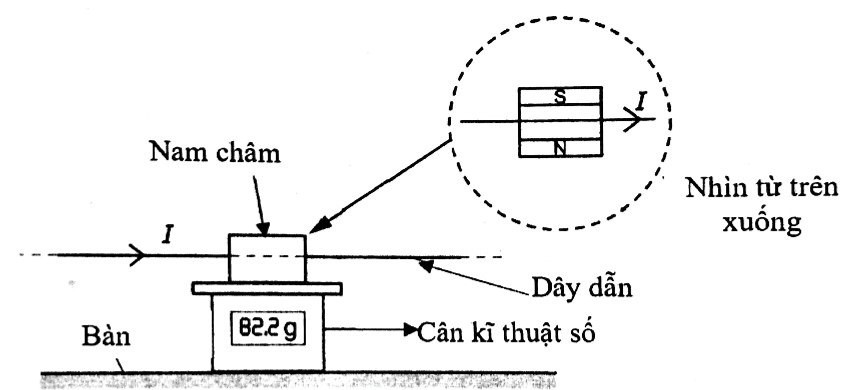
\includegraphics[width=0.6\linewidth]{figs/VN12-Y24-PH-SYL-018P-9}
	\end{center}
	Số liệu thu thập được như sau:
	\begin{itemize}
		\item Chiều dài của dây trong từ trường đều của nam châm: $\ell=\xsi{6,0\pm 0,2}{\centi\meter}$;
		\item Số chỉ của cân khi không có dòng điện trong dây dẫn: $\SI{80,0}{\gram}$;
		\item Số chỉ của cân khi có dòng điện trong dây: $\SI{82.2}{\gram}$;
		\item Dòng điện trong dây: $I=\xsi{5,0\pm0,1}{\ampere}$.
	\end{itemize}
	Viết kết quả đo giá trị của $B$. Bỏ qua sai số của cân.
	\loigiai{
		Dây dẫn đặt trong từ trường nam châm nên chịu tác dụng lực từ $F$.\\
		Lực $F$ hướng xuống tác dụng lên cân giống như một trọng lực $\mathrm{P}=\mathrm{mg}$.
		Với $m$ là chênh lệch số chỉ đọc ở cân khi có và không có dòng điện trong dây:
		$$
		\begin{aligned}
			& m=82,2-80,0=\SI{2.2}{\gram} \\
			& F=m g=2,2 \cdot 10^{-3} \cdot 9,8=\SI{0.0216}{\newton} \\
			& B=\frac{F}{I \ell \sin \alpha}=\frac{0,0216}{5,0.0,06 \cdot \sin \SI{90}{\degree}}\approx\SI{0.072}{\tesla}
		\end{aligned}
		$$
		
		Bỏ qua sai số của $F$ thì:
		$$
		\frac{\Delta B}{B}=\frac{\Delta I}{I}+\frac{\Delta \ell}{\ell} \Leftrightarrow \frac{\Delta B}{0,072}=\frac{0,1}{5}+\frac{0,2}{6} \Rightarrow \Delta B\approx0,004 T
		$$
		
		Kết quả đo: $B=\overline{B} \pm \Delta B=0,072 \pm \SI{0.004}{\tesla}$	
	}
\end{ex}\newpage
%	\let\lesson\undefined
\newcommand{\lesson}{\phantomlesson{Bài 10: Lực từ - Cảm ứng từ}}
\chapter[Cảm ứng từ gây ra bởi dòng điện trong dây dẫn có hình dạng đặc biệt (Đọc thêm)]{Cảm ứng từ gây ra bởi dòng điện trong dây dẫn có hình dạng đặc biệt (Đọc thêm)}
\section{Lý thuyết}
\subsection{Cảm ứng từ gây ra bởi dòng điện trong dây dẫn có hình dạng đặc biệt đặt trong không khí}
\subsubsection{Từ trường của dòng điện chạy trong dây dẫn thẳng, dài}
\begin{center}
	\begin{tikzpicture}
		\coordinate (O) at (0,0);
		\coordinate (M) at ($(O)+(-15:1.9)$);
		\coordinate (N) at ($(M)+(45:1.5)$);
		\node[draw, line width=1pt, fill=white, trapezium ,minimum width=8cm, trapezium left angle=60, trapezium right angle=120, anchor=center] at (O) {};
		\node[draw,blue, line width=1pt, fill=white, ellipse, minimum width=4cm, minimum height=2.5cm, anchor=center,
		decoration={markings, mark=at position 0.125 with {\arrow{stealth}}},
		decoration={markings, mark=at position 0.625 with {\arrow{stealth}}},
		postaction={decorate}
		] at (O) {};
		\tkzMarkRightAngle[draw=black,size=0.2](O,M,N);
		\draw[green!60!black, line width=1.5pt, decoration={markings, mark=at position 0.75 with {\arrow{stealth}}},
		postaction={decorate}] (O)--($(O)+(0,3)$);
		\draw[line width=1pt,dashed] (O)--(M);
		\draw[line width=1.5pt,green!60!black, dashed] (O)--($(O)-(0,1.5)$);
		\draw[green!60!black, line width=1.5pt] ($(O)-(0,1.5)$)--($(O)-(0,3)$);
		\draw[red, line width=1.5pt, -latex] (M)--($(M)+(45:1.5)$);
		\filldraw[black] (M) circle (2pt) node[below right] {M};
		\node[green!60!black, above right] at (0,2.25) {$I$};
		\node[red, above left] at (N) {$\vec{B}$};
		\node[above]  at ($(O)!0.5!(M)$) {$r$};
		
	\end{tikzpicture}
\end{center}
Độ lớn cảm ứng từ tại một điểm cách dòng điện thẳng dài vô hạn một đoạn $r$:
\begin{equation}
	B=2\cdot10^{-7}\dfrac{I}{r}
\end{equation}
\subsubsection{Từ trường của dòng điện chạy trong dây dẫn tròn}
\begin{center}
	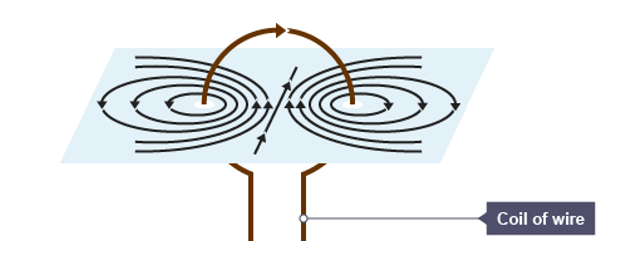
\includegraphics[width=0.4\linewidth]{../figs/VN12-Y24-PH-SYL-019-1}
\end{center}
Độ lớn cảm ứng từ tại tâm dòng điện tròn có $N$ vòng dây và có bán kính $R$:
\begin{equation}
	B=2\pi\cdot10^{-7}\dfrac{NI}{R}
\end{equation}
\subsubsection{Từ trường của ống dây có dòng diện chạy qua}
\begin{center}
	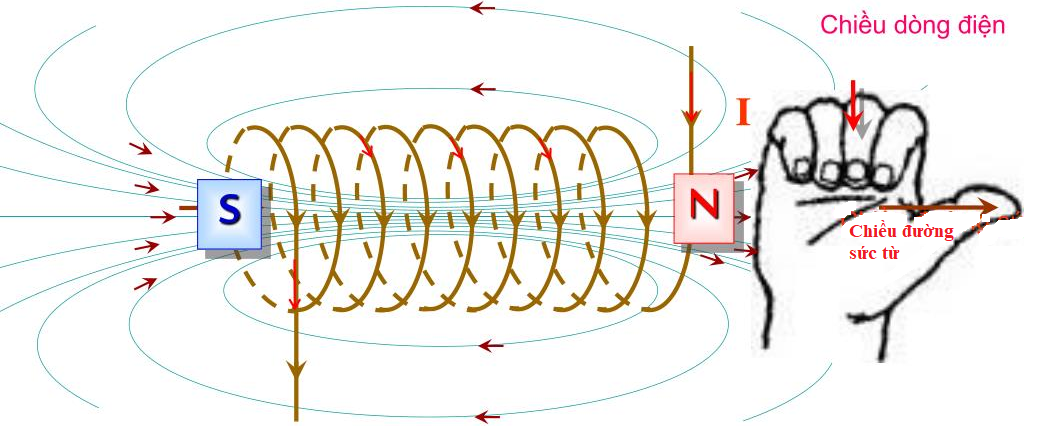
\includegraphics[width=0.6\linewidth]{../figs/VN12-Y24-PH-SYL-019-2}
\end{center}
Độ lớn cảm ứng từ bên trong ống dây có chiều dài $L$ và $N$ vòng dây (chiều dài ống dây rất lớn so với bán kính vòng dây):
\begin{equation}
	B=4\pi \cdot10^{-7}\dfrac{NI}{L}
\end{equation}
với $I$ là cường độ dòng điện trong dây dẫn.
\subsection{Nguyên lý chồng chất từ trường}
Xét hệ có $n$ dây dẫn lần lượt mang các dòng điện có cường độ dòng điện là $I_1$, $I_2$, \dots, $I_n$. Cảm ứng từ do mỗi dòng điện gây ra tại điểm M trong không gian là $\vec{B}_1$, $\vec{B}_2$,\dots,$\vec{B}_n$. Khi đó cảm ứng từ tổng hợp tại điểm M là:
\begin{equation}
	\vec{B}_\text{M}=\vec{B}_1+\vec{B}_2+\dots+\vec{B}_n
\end{equation}
\section{Mục tiêu bài học - Ví dụ minh hoạ}
\begin{dang}{Xác định được độ lớn cảm ứng từ do dòng điện trong dây dẫn có hình dạng đặc biệt gây ra}
	\viduii{2}
{Một dòng điện $\SI{20}{\ampere}$ chạy trong một dây dẫn thẳng, dài vô hạn, đặt trong không khí. Xác định độ lớn cảm ứng từ do dòng điện trong dây gây ra tại điểm cách dây $\SI{10}{\centi\meter}$.

}
{\hide{
Cảm ứng từ do dòng điện trong dây dẫn gây ra tại điểm cách dây đoạn $r=\SI{10}{\centi\meter}$:
$$B=2\cdot10^{-7}\dfrac{I}{r}=	2\cdot10^{-7}\cdot\dfrac{\left(\SI{20}{\ampere}\right)}{\left(\SI{0.1}{\meter}\right)}=\SI{4E-5}{\tesla}.$$

}

}

\viduii{2}
{Một vòng dây tròn bán kính $\SI{30}{\centi\meter}$ có dòng điện chạy qua. Cảm ứng từ do dòng điện gây ra tại tâm vòng dây có độ lớn $\SI{3.14E-5}{\tesla}$. Cường độ dòng điện chạy trong vòng dây là bao nhiêu?

}
{\hide{
Cảm ứng từ do dòng điện trong dây dẫn tròn gây ra tại tâm vòng dây:
$$B=2\pi\cdot10^{-7}\dfrac{I}{R}.$$
Cường độ dòng điện chạy trong vòng dây:
$$I=\dfrac{BR}{2\pi\cdot10^{-7}}=\dfrac{\left(\SI{3.14E-5}{\tesla}\right)\cdot\left(\SI{0.3}{\meter}\right)}{2\pi\cdot10^{-7}}=\SI{15}{\ampere}.$$
}

}
	
	\viduii{3}
	{Dùng một dây đồng có phủ một lớp sơn cách điện mỏng, quấn quanh một hình trụ dài $L=\SI{50}{\centi\meter}$, có đường kính $d=\SI{4}{\centi\meter}$ để làm một ống dây. Sợi dây quấn ống dây có chiều dài $\ell=\SI{314}{\centi\meter}$ và các vòng dây được quấn sát nhau. Hỏi nếu cho dòng điện cường độ $I=\SI{0.4}{\ampere}$ chạy qua ống dây, thì độ lớn cảm ứng từ bên trong ống dây bằng bao nhiêu?
	
}
{\hide{
Số vòng dây quấn trên ống dây:
$$N=\dfrac{\ell}{\pi d}.$$
Cảm ứng từ bên trong ống dây:
$$B=4\pi\cdot10^{-7}\dfrac{NI}{L}=4\cdot10^{-7}\dfrac{\ell I}{ Ld}=4\cdot10^{-7}\dfrac{\left(\SI{3.14}{\meter}\right)\cdot\left(\SI{0.4}{\ampere}\right)}{\left(\SI{4E-2}{\meter}\right)\cdot\left(\SI{0.5}{\meter}\right)}=\SI{2.512E-5}{\tesla}.$$	

}

}
\end{dang}
\begin{dang}{Xác định được cảm ứng từ tổng hợp}
	\viduii{3}
	{Hai dây dẫn thẳng, rất dài, đặt song song, cách nhau $\SI{10}{\centi\meter}$ trong không khí, có hai dòng điện ngược chiều, có cường độ $I_1=\SI{6}{\ampere}$; $I_2=\SI{12}{\ampere}$ chạy qua. Xác định cảm ứng từ tổng hợp do hai dòng điện này gây ra tại điểm M cách dây dẫn mang dòng $I_1$ đoạn $\SI{5}{\centi\meter}$ và cách dây dẫn mang dòng $I_2$ đoạn $\SI{15}{\centi\meter}$.
	
}
{\hide{
\begin{center}
	\begin{tikzpicture}
		\coordinate (A) at (0,0);
		\coordinate (B) at (10,0);
		\coordinate (M) at (-5,0);
		
	
		\draw[red, line width=1.5pt, -stealth] (M)--($(M)+(0,-3)$);
		\draw[green!60!black, line width=1.5pt, -stealth] (M)--($(M)+(0,2)$);
		\draw[blue, line width=1.5pt, -stealth] (M)--($(M)+(0,-1)$);
		\draw[line width=1pt, dashed] (M)--(B);
		\node[circle, red, fill=white, inner sep=0pt, minimum size=0pt] at (A) {\LARGE$\odot$};
		\node[below] at ($(A)+(0,-.25)$)  {A};
		\node[below] at ($(B)+(0,-.25)$)  {B};
		\node[above] at ($(A)+(0,0.25)$)  {$I_1$};
		\node[above] at ($(B)+(0,.25)$)  {$I_2$};
		\node[red, left] at ($(M)-(0,3)$) {$\vec{B}_{1M}$};
		\node[green!60!black, left] at ($(M)+(0,2)$) {$\vec{B}_{2M}$};
		\node[blue, left] at ($(M)+(0,-1)$) {$\vec{B}_M$};
		\node[circle, green!60!black, fill=white, inner sep=0pt, minimum size=0pt] at (B) {\LARGE$\otimes$};
			\filldraw[black] (M) circle (2pt) node[left] {M};
	\end{tikzpicture}
\end{center}	
Từ trường do các dây dẫn gây ra tại M:
\begin{align*}
	\begin{cases}
		B_{1M}=\SI{2E-7}{}\dfrac{I_1}{\text{AM}}=\SI{2E-7}{}\dfrac{\left(\SI{6}{\ampere}\right)}{\SI{5E-2}{\meter}}=\SI{2.4E-5}{\tesla}\\
		\ \\
		B_{2M}=\SI{2E-7}{}\dfrac{I_2}{\text{BM}}=\SI{2E-7}{}\dfrac{\left(\SI{12}{\ampere}\right)}{\SI{15E-2}{\meter}}=\SI{1.6E-5}{\tesla}
	\end{cases}
\end{align*}
Vì $\vec{B}_{1M}\uparrow\downarrow\vec{B}_{2M}$ nên:
$$B_M=\left|B_{1M}-B_{2M}\right|=\SI{0.8E-5}{\tesla}.$$
}

}

\viduii{3}
{Hai dây dẫn thẳng, rất dài, đặt song song, cách nhau $\SI{15}{\centi\meter}$ trong không khí, có hai dòng điện cùng chiều, cùng cường độ $I_1=\SI{10}{\ampere}$, $I_2=\SI{5}{\ampere}$ chạy qua. Xác định điểm M mà tại đó cảm ứng từ tổng hợp do hai dòng điện này gây ra bằng 0.

}
{\hide{
		Để từ trường tổng hợp tại M bằng 0 thì:
		$$\vec{B}_M=\vec{B}_{1M}+\vec{B}_{2M}=\vec{0}\Rightarrow \vec{B}_{1M}=-\vec{B}_{2M}.$$	
	\begin{center}
		\begin{tikzpicture}
			\coordinate (A) at (0,0);
			\coordinate (B) at (15,0);
			\coordinate (M) at (10,0);
			
			\draw[line width=1pt, dashed] (A)--(B);
			\draw[red, line width=1.5pt,-stealth] (M)--($(M)+(0,2)$);
			
			\draw[green!60!black, line width=1.5pt,-stealth] (M)--($(M)-(0,2)$);
			\node[circle, green!60!black, fill=white, inner sep=0pt, minimum size=0pt] at (A) {\LARGE$\otimes$};
			\node[circle, red, fill=white, inner sep=0pt, minimum size=0pt] at (B) {\LARGE$\otimes$};
			\node[below] at ($(A)-(0,0.25)$) {A};
			\node[below] at ($(B)-(0,0.25)$) {B};
			\node[above] at ($(A)+(0,0.25)$) {$I_1$};
			\node[above] at ($(B)+(0,0.25)$) {$I_2$};
			\node[left, red] at ($(M)+(0,2)$) {$\vec{B}_{2M}$};
			\node[left, green!60!black] at ($(M)-(0,2)$) {$\vec{B}_{1M}$};
			\filldraw[black] (M) circle(2pt) node[above left] {M};
			
		\end{tikzpicture}
	\end{center}
Do hai dòng điện cùng chiều nên điểm M phải nằm trong khoảng AB:
\begin{eqnarray*}
	&&B_{1M}=B_{2M}\\
	&\Rightarrow& \dfrac{I_1}{\text{AM}}=\dfrac{I_2}{\text{BM}}\\
	&\Rightarrow& \text{AM}=2\text{BM}.
\end{eqnarray*}
Mà $\text{AM}+\text{BM}=\text{AB}=\SI{15}{\centi\meter}$ nên:
\begin{align*}
	\begin{cases}
		\text{AM}=\SI{10}{\centi\meter}\\
		\text{BM}=\SI{5}{\centi\meter}
	\end{cases}
\end{align*}
}

}
	\viduii{3}
	{Hai dây dẫn thẳng, rất dài, đặt song song, cách nhau $\SI{10}{\centi\meter}$ trong không khí có hai dòng điện cùng chiều, có cường độ $I_1=\SI{9}{\ampere}$; $I_2=\SI{16}{\ampere}$ chạy qua. Xác định cảm ứng từ tổng hợp do hai dòng điện này gây ra tại điểm M cách dây dẫn mang dòng điện $I_1$ đoạn $\SI{6}{\centi\meter}$ và cách dây dẫn mang dòng điện $I_2$ đoạn $\SI{8}{\centi\meter}$.
	
}
{\hide{
\begin{center}
	\begin{tikzpicture}
		\coordinate (A) at (0,0);
		\coordinate (B) at (7.5,0);
		\coordinate (C) at ($(A)+(53.13:4.5)$);
		\coordinate (D) at ($(C)+(143.13:1.5)$);
		\coordinate (E) at ($(C)+(-126.87:2)$);
		\draw[line width=1pt, dashed] (A)--(B)--(C)--(A);
		\node[circle,red,fill=white,inner sep=0pt,minimum size=0pt] at (A) {\LARGE$\odot$};
		\node[circle,green!60!black,fill=white,inner sep=0pt,minimum size=0pt] at (B) {\LARGE$\odot$};
		\tkzMarkRightAngle[size=0.3,color=blue](A,C,B);
		\draw[red, line width=1.5pt,-stealth] (C)--(D);
		\draw[green!60!black, line width=1.5pt,-stealth] (C)--(E);
		\draw[line width=1pt,blue, dashed] (D)--($(D)+(-126.87:2)$)--(E);
		\draw[blue, line width=1.5pt,-stealth] (C)--($(D)+(-126.87:2)$);
		\node[below] at ($(A)-(0,0.25)$) {A};
		\node[below] at ($(B)-(0,0.25)$) {B};
		\node[above] at (D) {$\vec{B}_{1C}$};
		\node[right] at (E) {$\vec{B}_{2C}$};
		\node[left] at ($(D)+(-126.87:2)$) {$\vec{B}_C$};
		\node[above right] at (C) {C};
		\node[left] at ($(A)+(-0.25,0)$) {$I_1$};
		\node[right] at ($(B)+(0.25,0)$) {$I_2$};
	\end{tikzpicture}
\end{center}	
Từ trường do mỗi dòng điện gây ra tại C:
\begin{align*}
	\begin{cases}
		B_{1C}=\SI{2E-7}{}\dfrac{I_1}{\text{AC}}=\SI{2E-7}{}\dfrac{\left(\SI{9}{\ampere}\right)}{\SI{6e-2}{\meter}}=\SI{3E-5}{\tesla}\\
		\ \\
		B_{2C}=\SI{2E-7}{}\dfrac{I_2}{\text{BC}}=\SI{2E-7}{}\dfrac{\left(\SI{16}{\ampere}\right)}{\SI{8e-2}{\meter}}=\SI{4E-5}{\tesla}
	\end{cases}
\end{align*}
Vì $\vec{B}_{1C}\bot\vec{B}_{2C}$ nên:
$$B_C=\sqrt{B^2_{1C}+B^2_{2C}}=\SI{5E-5}{\tesla}.$$
}

}
\end{dang}\newpage
%	\section{Hiện tượng cảm ứng điện từ}
\subsection{Tóm tắt lí thuyết}
\begin{tomtat}
	\subsubsection{Từ thông}
	\begin{center}
		\begin{tikzpicture}
			\coordinate (O) at (0,0);
			\coordinate (A) at ($(O)+(45:2)$);
			\coordinate (B) at (4,0);
			\foreach \i in {-2,-1,...,2}{
				\draw[blue, line width=1.5pt] (-3,\i)--+(0:{-\i+2.8});
				
			}
			\draw[rotate around={-45:(O)},black, line width=1.5pt, fill=green!20!white](O) ellipse (3cm and 1.25cm);
			\foreach \i in {-2,-1,...,2}{
				\draw[blue, line width=1.5pt, -stealth] (-\i,\i)--(4,\i);	
			}
			\draw[red, -stealth, line width=1.5pt] (O)--(A);
			\fill[black] (O) circle (2pt) node [left] {O};
			\tkzMarkAngle[size=0.75cm,color=purple,line width=1.5pt](B,O,A);
			\tkzLabelAngle[color=black,pos=1.0, purple](B,O,A){$\alpha$};
			\node[blue, above] at (B) {$\vec{B}$};
			\node[red, above] at (A) {$\vec{n}$};
			\node[right] at (-0.25,-1) {$S$};
		\end{tikzpicture}
	\end{center}
	\begin{dn}
		Từ thông là đại lượng đặc trưng cho số đường sức từ xuyên qua diện tích $S$ và được xác định bởi biểu thức:
		\begin{equation}
			\Phi=BS\cos\alpha
		\end{equation}
	\end{dn}
	Trong hệ SI, từ thông có đơn vị là weber $\left(\si{\weber}\right)$.
	$$\SI{1}{\weber}=\SI{1}{\tesla\cdot\meter^2}.$$
	Trong đó:
	\begin{itemize}
		\item $\Phi$: từ thông, đơn vị trong hệ SI là weber $\left(\si{\weber}\right)$;
		\item $B$: cảm ứng từ, đơn vị trong hệ SI là tesla $\left(\si{\tesla}\right)$;
		\item $S$: diện tích mặt kín ($\si{\meter^2}$);
		\item $\alpha=\left(\vec{B},\vec{n}\right)$: góc hợp bởi vector cảm ứng từ $\vec{B}$ và vector pháp tuyến $\vec{n}$ của mặt kín.
	\end{itemize}
	\begin{luuy}
		Nếu khung dây có $N$ vòng dây được đặt trong từ trường đều, thì từ thông qua khung dây được xác định bởi biểu thức:
		$$\Phi=NBS\cos\alpha.$$
	\end{luuy}
	\subsubsection{Hiện tượng cảm ứng điện từ}
	\paragraph{Khái niệm hiện tượng cảm ứng điện từ}
	\begin{dn}
		Khi từ thông qua mặt giới hạn bởi một khung dây dẫn kín biến thiên thì trong khung dây xuất hiện dòng điện cảm ứng. Hiện tượng này được gọi là hiện tượng cảm ứng điện từ.
	\end{dn}
	\paragraph{Định luật Lenz về chiều dòng điện cảm ứng}
	\begin{dl}
		Dòng điện cảm ứng qua khung dây dẫn kín có chiều sao cho từ trường do nó sinh ra (từ trường cảm ứng) có tác dụng chống lại sự biến thiên từ thông qua chính khung dây đó.
	\end{dl}
	\begin{center}
		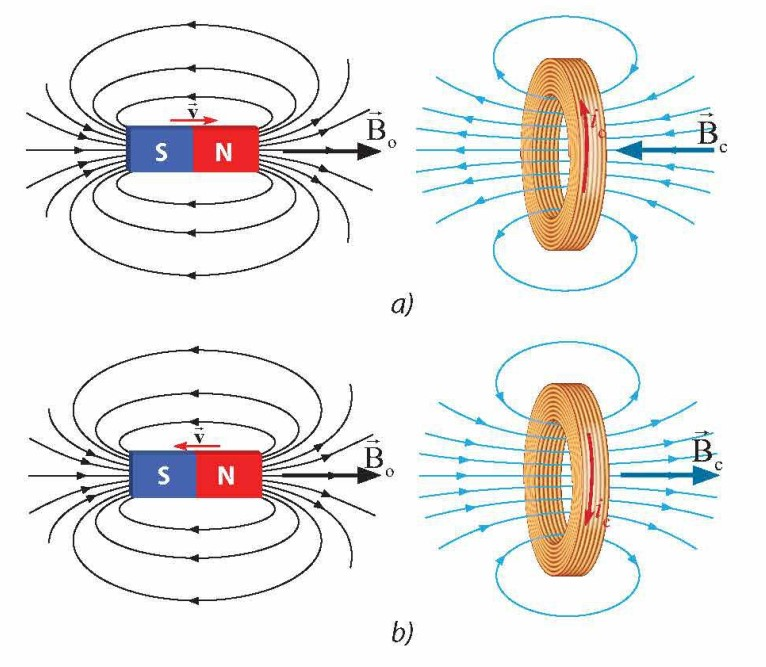
\includegraphics[width=0.45\linewidth]{figs/VN12-Y24-PH-SYL-020-1}
		\captionof{figure}{Chiều dòng điện cảm ứng $i_c$ qua khung dây dẫn kín khi đưa nam châm (a) lại gần và (b) ra xa khung dây}
	\end{center}
	\subsubsection{Định luật Faraday về suất điện động cảm ứng}
	\begin{dl}
		Độ lớn suất điện động cảm ứng trong khung dây dẫn kín tỉ lệ với tốc độ biến thiên từ thông qua diện tích giới hạn bởi khung dây.\\
		Trong hệ SI, độ lớn suất điện động cảm ứng được xác định bằng biểu thức:
		\begin{equation}
			\left|e_c\right|=\left|\dfrac{\Delta \Phi}{\Delta t}\right|
		\end{equation}
	\end{dl}
	Trong đó:
	\begin{itemize}
		\item $\left|e_c\right|$: độ lớn suất điện động cảm ứng, đơn vị trong hệ SI là volt $\left(\si{\volt}\right)$;
		\item $\Delta\Phi$: độ biến thiên từ thông, đơn vị trong hệ SI là weber $\left(\si{\weber}\right)$;
		\item $\Delta t$: khoảng thời gian từ thông biến thiên, đơn vị trong hệ SI là giây $\left(\si{\second}\right)$.
	\end{itemize}
	\begin{luuy}
		Khi kết hợp với nội dung định luật Lenz, biểu thức định luật Faraday được viết lại:
		\begin{equation}
			e_c=-\dfrac{\Delta \Phi}{\Delta t}
		\end{equation}
		Trong trường hợp khung dây có $N$ vòng dây thì:
		\begin{equation}
			e_c=-N\dfrac{\Delta \Phi}{\Delta t}
		\end{equation}
	\end{luuy}
	\subsubsection{Một số ứng dụng của hiện tượng cảm ứng điện từ}
	\paragraph{Guitar điện}
	\begin{minipage}{0.5\textwidth}
		Bộ cảm ứng (pickup) của guitar điện gồm một cuộn dây và một nam châm vĩnh cửu, được đặt gần dây đàn guitar bằng kim loại có thể nhiễm từ. Khi gảy đàn, đoạn dây gần nam châm bị nhiễm từ, dao động và tạo ra sự biến thiên từ thông qua cuộn dây của bộ cảm ứng, từ đó tạo ra suất điện động cảm ứng. Tín hiệu điện được đưa đến một bộ khuếch đại và loa, tạo ra sóng âm thanh mà chúng ta nghe được.
	\end{minipage}
	\hfill
	\begin{minipage}{0.5\textwidth}
		\centering
		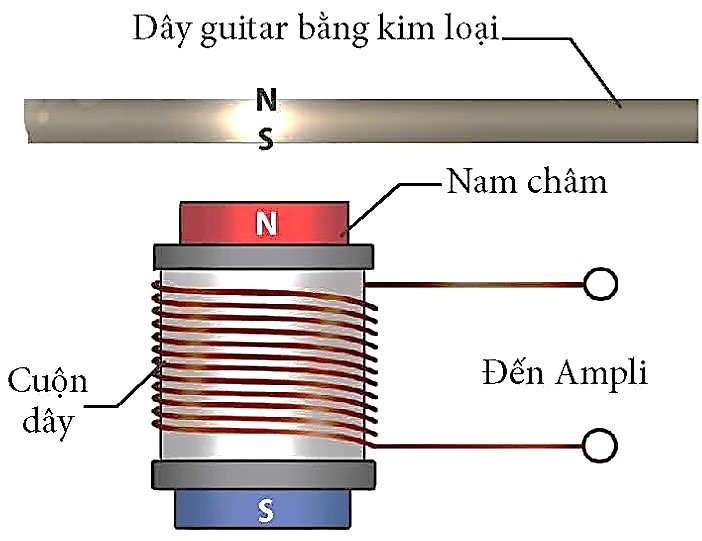
\includegraphics[width=0.55\linewidth]{figs/VN12-Y24-PH-SYL-021-1}
	\end{minipage}
	\paragraph{Dynamo xe đạp}
	Khi bánh xe quay, núm dẫn  động và nam châm cũng quay theo, do đó từ thông qua cuộn dây biến thiên. Lúc này, trong cuộn dây xuất hiện dòng điện cảm ứng và thắp sáng bóng đèn.
	\begin{center}
		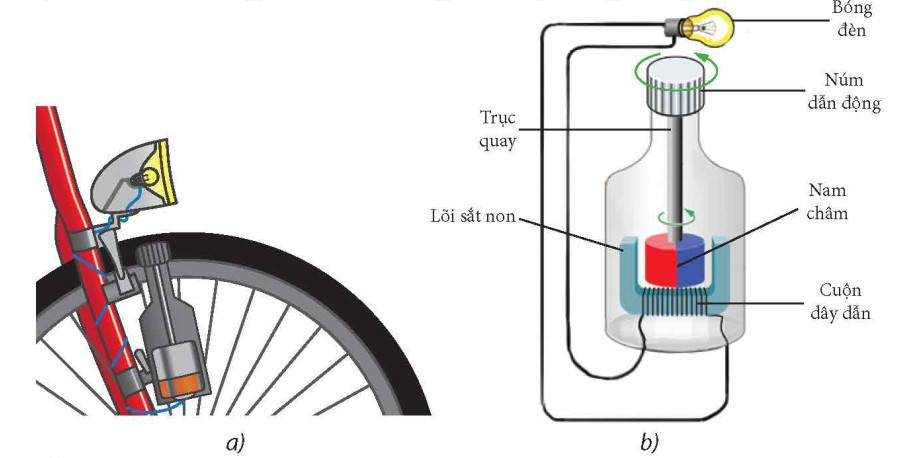
\includegraphics[width=0.6\linewidth]{figs/VN12-Y24-PH-SYL-021-2}
		\captionof{figure}{a) Dynamo trên xe đạp; b) Cấu tạo của dynamo trên xe đạp.}
	\end{center}
	\subsubsection{Mô hình sóng điện từ}
	\paragraph{Điện từ trường}
	\begin{dn}
		Trong vùng không gian có từ trường biến thiên theo thời gian thì trong vùng đó xuất hiện một điện trường xoáy; ngược lại, trong vùng không gian có điện trường biến thiên theo thời gian thì trong vùng đó xuất hiện một từ trường biến thiên theo thời gian. Do đó, điện trường biến thiên và từ trường biến thiên theo thời gian chuyển hoá lẫn nhau và cùng tồn tại trong không gian, được gọi là điện từ trường.
	\end{dn}
	\begin{center}
		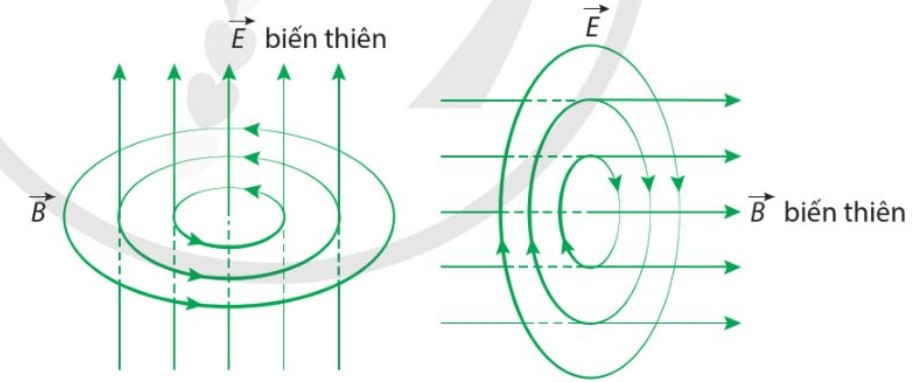
\includegraphics[width=0.6\linewidth]{figs/VN12-Y24-PH-SYL-021-3}
		\captionof{figure}{a) Điện trường biến thiên gây ra từ trường biến thiên; b) Từ trường biến thiên gây ra điện trường biến thiên.}
	\end{center}
	\paragraph{Mô hình sóng điện từ}
	\begin{center}
		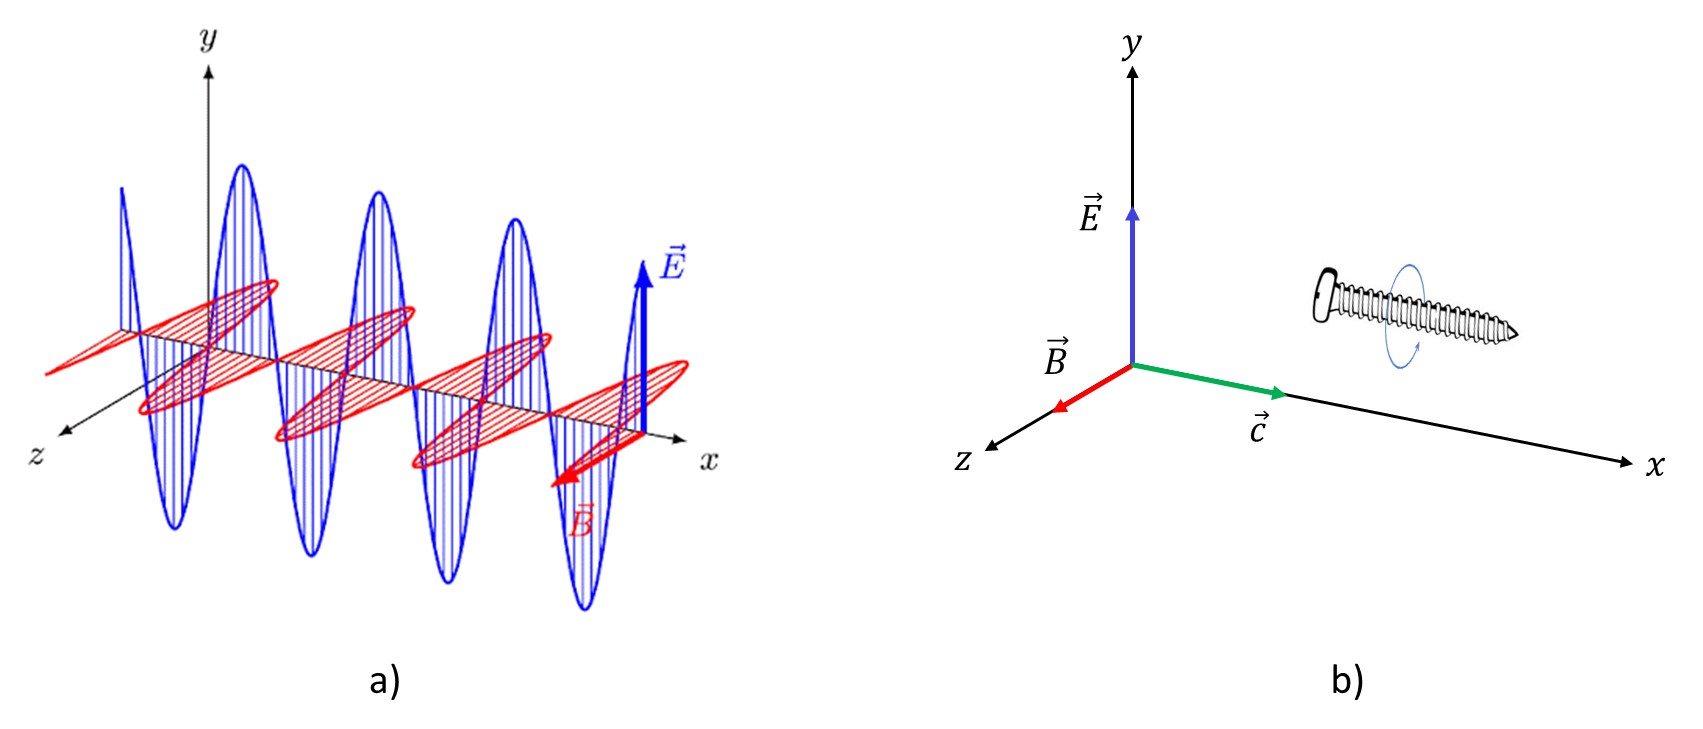
\includegraphics[width=0.8\linewidth]{figs/VN12-Y24-PH-SYL-021-4}
		\captionof{figure}{a) Mô hình sự lan truyền sóng điện từ; b) Minh hoạ quy tắc vặn đinh ốc.}
	\end{center}
	Trong quá trình lan truyền sóng điện từ, tại một điểm có
	\begin{itemize}
		\item vector cường độ điện trường $\vec{E}$ và vector cảm ứng từ $\vec{B}$ luôn vuông góc với nhau và vuông góc với phương truyền sóng $\Rightarrow $ sóng điện từ là sóng ngang;
		\item điện trường và từ trường biến thiên cùng pha.
	\end{itemize}
\begin{noidung}{Quy tắc vặn đinh ốc để xác định chiều truyền sóng điện từ}
	Quay đinh ốc theo chiều từ vector cường độ điện trường đến vector cảm ứng từ thì chiều tiến của đinh ốc là chiều lan truyền của sóng điện từ.
\end{noidung}
\end{tomtat}

\subsection{Ví dụ minh hoạ}
\begin{dang}{Xác định từ thông gửi qua khung dây}
	\end{dang}
\begin{vd}
		Một vòng dây phẳng giới hạn diện tích $S=\SI{5}{\centi\meter^2}$ đặt trong từ trường đều có cảm ứng từ $B=\SI{0.1}{\tesla}$. Mặt phẳng vòng dây làm thành với $\vec{B}$ một góc $\alpha=\SI{30}{\degree}$. Tính từ thông qua $S$.
		\loigiai{Góc hợp bởi $\vec{B}$ và vector pháp tuyến $\vec{n}$ của mặt phẳng khung dây $\left(\vec{B},\vec{n}\right)=\SI{90}{\degree}-\alpha=\SI{60}{\degree}.$\\
			Từ thông qua tiết diện $S$:
			$$\Phi=BS\cos\left(\vec{B}, \vec{n}\right)=\left(\SI{0.1}{\tesla}\right)\cdot\left(\SI{5E-4}{\meter^2}\right)\cos\SI{60}{\degree}=\SI{2.5E-5}{\weber}.$$}
\end{vd}
% ==================================
\begin{vd}
		Một khung dây phẳng giới hạn diện tích $S=\SI{5}{\centi\meter^2}$ gồm 20 vòng dây đặt trong từ trường đều  có cảm ứng từ $B=\SI{0.1}{\tesla}$ sao cho mặt phẳng khung dây hợp với vector cảm ứng từ một góc $\SI{60}{\degree}$. Tính từ thông qua diện tích giới hạn bởi khung dây.
		\loigiai{Góc hợp bởi vector cảm ứng từ $\vec{B}$ và vector pháp tuyến $\vec{n}$ là $\left(\vec{B},\vec{n}\right)=\SI{90}{\degree}-\SI{60}{\degree}=\SI{30}{\degree}.$\\
			Từ thông qua diện tích giới hạn bởi khung dây:
			$$\Phi=NBS\cos\left(\vec{B},\vec{n}\right)=\SI{8.66E-4}{\weber}.$$}
\end{vd}

\begin{dang}{Vận dụng định luật Lenz xác định chiều dòng điện cảm ứng}
	\end{dang}
% ====================
\begin{vd}
		Đặt một thanh nam châm thẳng ở gần một khung dây kín ABCD như hình vẽ.
		\begin{center}
			\begin{tikzpicture}
				\coordinate (B) at (0,0);
				\coordinate (A) at (0,-3);
				\coordinate (C) at (2,1);
				\coordinate (D) at (2,-2);
				\coordinate (N) at (-3cm,-1cm);
				\coordinate (S) at (-2cm,-1cm);
				\draw[dashed, line width=1pt] (S)--(3,-1);
				\node[draw,color= blue!75!black, line width=1.5pt, fill=blue!75!black, rectangle, minimum width=1cm, minimum height=0.4cm, anchor=center] at(N) {};
				\node[draw,color= blue!75!black, line width=1.5pt, fill=white, rectangle, minimum width=1cm, minimum height=0.4cm, anchor=center] at(S) {};
				\draw[line width=1.5pt] (C)--(B)--(A)--(D);
				\draw[line width=1.5pt, dashed] (C)--(D);
				\node[left] at (A) {A};
				\node[left] at (B) {B};
				\node[right] at (C) {C};
				\node[right] at (D) {D};
				\node[color=white] at (N) {\bfseries N};
				\node[color=blue!75!black] at (S) {\bfseries S};
			\end{tikzpicture}
		\end{center}
		Xác định chiều của dòng điện cảm ứng xuất hiện trong khung dây trong các trường hợp sau:
		\begin{enumerate}[label=\alph*)]
			\item Đưa nam châm lại gần khung dây.
			\item Kéo nam châm ra xa khung dây.
		\end{enumerate}
		\loigiai{\begin{enumerate}[label=\alph*)]
				\item Đưa nam châm lại gần khung dây, từ thông qua khung dây tăng nên $\vec{B}_c\uparrow\downarrow \vec{B}_0$.
				\begin{center}
					\begin{tikzpicture}
						\coordinate (B) at (0,0);
						\coordinate (A) at (0,-3);
						\coordinate (C) at (2,1);
						\coordinate (D) at (2,-2);
						\coordinate (N) at (-3cm,-1cm);
						\coordinate (S) at (-2cm,-1cm);
						\draw[dashed, line width=1pt] (S)--(3,-1);
						\draw[-stealth, blue, line width=1.5pt] (N)--+(-2,0);
						\draw[-stealth, line width=1.5pt] (S)--+(1.5,0);
						\draw[-stealth, red, line width=1.5pt] (1,-1)--+(1.5,0);
						\node[draw,color= blue!75!black, line width=1.5pt, fill=blue!75!black, rectangle, minimum width=1cm, minimum height=0.4cm, anchor=center] at(N) {};
						\node[draw,color= blue!75!black, line width=1.5pt, fill=white, rectangle, minimum width=1cm, minimum height=0.4cm, anchor=center] at(S) {};
						\draw[line width=1.5pt,decoration={markings, mark=at position 0.5 with {\arrow{stealth}}},
						postaction={decorate}
						] (C)--(B)--(A)--(D);
						\draw[line width=1.5pt, dashed] (C)--(D);
						\node[above,blue] at ($(N)+(-2,0)$) {$\vec{B}_0$};
						\node[above] at ($(S)+(1.5,0)$) {$\vec{v}_0$};
						\node[above, red] at (2.5,-1) {$\vec{B}_c$};
						\node[right] at ($(A)!0.5!(B)$) {$i_c$};
						\node[left] at (A) {A};
						\node[left] at (B) {B};
						\node[right] at (C) {C};
						\node[right] at (D) {D};
						\node[color=white] at (N) {\bfseries N};
						\node[color=blue!75!black] at (S) {\bfseries S};
					\end{tikzpicture}
				\end{center}
				\item Đưa nam châm ra xa khung dây, từ thông qua khung dây giảm nên $\vec{B}_c\uparrow\uparrow \vec{B}_0$.
				\begin{center}
					\begin{tikzpicture}
						\coordinate (B) at (0,0);
						\coordinate (A) at (0,-3);
						\coordinate (C) at (2,1);
						\coordinate (D) at (2,-2);
						\coordinate (N) at (-3cm,-1cm);
						\coordinate (S) at (-2cm,-1cm);
						\draw[dashed, line width=1pt] (S)--(3,-1);
						\draw[-stealth, blue, line width=1.5pt] (N)--+(-2,0);
						\draw[-stealth, line width=1.5pt] (N)--+(-1,0);
						\draw[-stealth, red, line width=1.5pt] (1,-1)--+(-1.5,0);
						\node[draw,color= blue!75!black, line width=1.5pt, fill=blue!75!black, rectangle, minimum width=1cm, minimum height=0.4cm, anchor=center] at(N) {};
						\node[draw,color= blue!75!black, line width=1.5pt, fill=white, rectangle, minimum width=1cm, minimum height=0.4cm, anchor=center] at(S) {};
						\draw[line width=1.5pt,decoration={markings, mark=at position 0.5 with {\arrow{stealth}}},
						postaction={decorate}
						] (D)--(A)--(B)--(C);
						\draw[line width=1.5pt, dashed] (C)--(D);
						\node[above,blue] at ($(N)+(-2,0)$) {$\vec{B}_0$};
						\node[above] at ($(N)+(-1,0)$) {$\vec{v}_0$};
						\node[above, red] at (-0.5,-1) {$\vec{B}_c$};
						\node[right] at ($(A)!0.5!(B)$) {$i_c$};
						\node[left] at (A) {A};
						\node[left] at (B) {B};
						\node[right] at (C) {C};
						\node[right] at (D) {D};
						\node[color=white] at (N) {\bfseries N};
						\node[color=blue!75!black] at (S) {\bfseries S};
					\end{tikzpicture}
				\end{center}
		\end{enumerate}	}
\end{vd}
% ================================
\begin{vd}
		Xác định chiều dòng điện cảm ứng xuất hiện trong mạch ABCD khi dịch chuyển mạch ABCD ra xa dòng điện $I$ thẳng, dài vô hạn. Biết mạch ABCD và dòng điện $I$ luôn nằm trong cùng mặt phẳng.
		\begin{center}
			\begin{tikzpicture}
				\coordinate(O) at(0,0);
				\node[draw, rectangle, line width=1.5pt, minimum height=3cm, minimum width=2cm] at (O) {};
				\draw[line width=1.5pt, blue, decoration={markings, mark=at position 0.5 with {\arrow{stealth}}},
				postaction={decorate}
				] (-2,-3)--(-2,3);
				\draw[line width=1.5pt, -stealth] (1,0)--+(1,0);
				\node[left,blue] at(-2,0) {$I$};
				\node[above] at (2,0) {$\vec{v}_0$};
				\node[above] at (-1,1.5) {A};
				\node[above] at (1,1.5) {B};
				\node[below] at (1,-1.5) {C};
				\node[below] at (-1,-1.5) {D};
			\end{tikzpicture}
		\end{center}
		\loigiai{\begin{center}
				\begin{tabular}{M{5cm}L{11cm}}
					\begin{tikzpicture}
						\coordinate(O) at(0,0);
						\node[draw, rectangle, line width=1.5pt, minimum height=3cm, minimum width=2cm, decoration={markings, mark=at position 0.1 with {\arrowreversed{stealth}}},
						decoration={markings, mark=at position 0.6 with {\arrowreversed{stealth}}},
						postaction={decorate}] at (O) {};
						\draw[line width=1.5pt, blue, decoration={markings, mark=at position 0.5 with {\arrow{stealth}}},
						postaction={decorate}
						] (-2,-2)--(-2,2);
						\draw[line width=1.5pt, -stealth] (1,0)--+(1,0);
						\node[blue] at (0,-0.5) {\LARGE$\otimes$};
						\node[red] at (0,0.5) {\LARGE$\otimes$};
						\node[blue, right] at (0.25,-0.5) {$\vec{B}_0$};
						\node[red, right] at (0.25,0.5) {$\vec{B}_c$};
						\node[left,blue] at(-2,0) {$I$};
						\node[above] at (2,0) {$\vec{v}_0$};
						\node[above] at (-1,1.5) {A};
						\node[above] at (1,1.5) {B};
						\node[below] at (1,-1.5) {C};
						\node[below] at (-1,-1.5) {D};
						\node[above] at (0,1.5) {$i_c$};
					\end{tikzpicture} & Dòng điện thẳng $I$ gây ra trong mạch ABCD từ trường  có các đường cảm ứng từ $\vec{B}_0$  hướng vào mặt phẳng ABCD.\newline
					Khi di chuyển khung ra xa dây, từ thông qua mạch giảm nên $\vec{B}_c$ do $i_c$ tạo ra cùng chiều $\vec{B}_0$. Do đó, mặt ABCD là mặt Nam nên $i_c$ cùng chiều kim đồng hồ theo chiều ABCD.\\
				\end{tabular}
			\end{center}
		}
\end{vd}
\begin{dang}{Giải thích được một số ứng dụng của hiện tượng cảm ứng điện từ}
\end{dang}
\begin{vd}
		Cho một đĩa kim loại dao động trong không khí, đĩa sẽ dao động trong một thời gian xác định. Khi cho đĩa dao động giữa hai cực từ của một nam châm thì thời gian đĩa dao động sẽ ngắn hơn. Hiện tượng này được ứng dùng để hãm chuyển động, đặc biệt là chuyển động quay của một bộ phận nào đó trong một số thiết bị. Em hãy giải thích cơ chế của hiện tượng trên.
		\begin{center}
			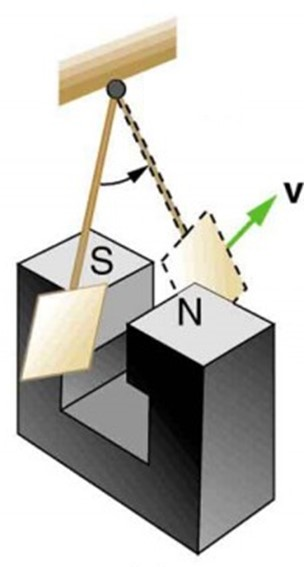
\includegraphics[width=0.15\linewidth]{figs/VN12-Y24-PH-SYL-021-5}
		\end{center}
		\loigiai{Khi đĩa đi vào từ trường, nó cắt các đường sức từ và do đó trong đĩa xuất hiện suất điện động cảm ứng. Vì đĩa là chất dẫn điện nên suất điện động cảm ứng tạo ra dòng điện trong đĩa. Những dòng điện này được gọi là dòng điện xoáy (dòng điện Foucault). Chúng có đặc điểm là chạy theo các đường cong kín trong khối vật dẫn.\\
			Theo định luật Lenz, các dòng điện cảm ứng chạy trong đĩa sẽ tạo ra lực cản trở chuyển động, làm cho dao động bị tắt dần nhanh.}
\end{vd}
% =====================================
\begin{vd}
		Hình bên là một đèn pin có thể được sạc lại bằng cách lắc đèn pin theo trục dọc của nó.
		\begin{center}
			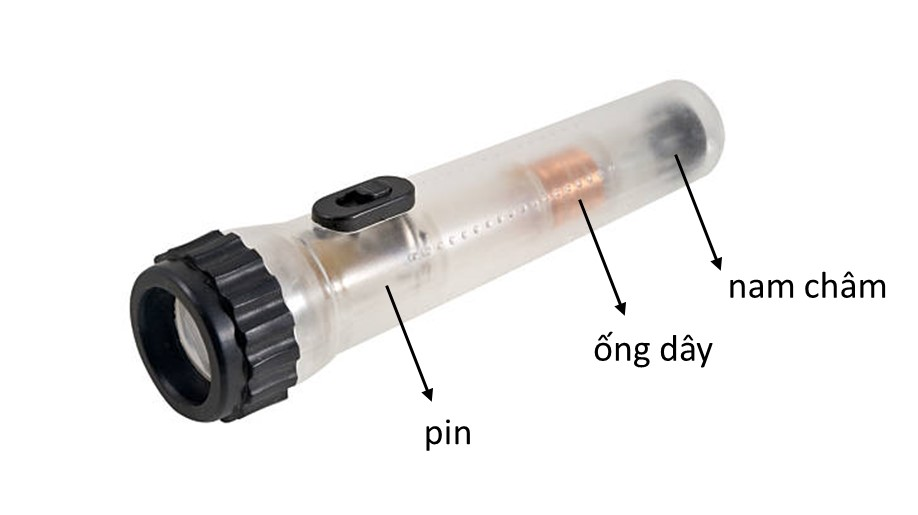
\includegraphics[width=0.4\linewidth]{figs/VN12-Y24-PH-SYL-021-6}
		\end{center}
		\begin{enumerate}[label=\alph*)]
			\item Tại sao khi lắc đèn thì pin được sạc (nạp điện)?
			\item Nêu cách để thời gian sạc nhanh hơn.
		\end{enumerate}
		\loigiai{\begin{enumerate}[label=\alph*)]
				\item Khi lắc đèn pin, nam châm sẽ dao động qua lại trong cuộn dây, làm từ trường qua cuộn dây tăng giảm dẫn đến từ thông qua cuộn dây biến đổi và làm xuất hiện suất điện động cảm ứng trong cuộn dây. Suất điện động này gây ra hiệu điện thế ở hai đầu cuộn dây. Hiệu điện thế này tạo ra dòng điện để sạc điện cho pin.
				\item Để thời gian sạc nhanh hơn cần tăng hiệu điện thế, bằng cách:
				\begin{itemize}
					\item Cách 1: Cho nam châm chuyển động nhanh hơn (lắc nhanh);
					\item Cách 2: Tăng số vòng dây trên cuộn dây hoặc từ trường của nam châm mạnh hơn. Cách này phụ thuộc vào nhà sản xuất đèn pin.
				\end{itemize}
		\end{enumerate}	}
\end{vd}
\begin{dang}{Vận dụng định luật Faraday tính được suất điện động cảm ứng}
\end{dang}
\begin{vd}
	Một đĩa kim loại được chế tạo để quay với tốc độ 20 vòng/giây quanh một trục đi qua tâm và vuông góc với mặt phẳng của nó. Đĩa được đặt trong từ trường đều có độ lớn cảm ứng từ là $\SI{0.2}{\tesla}$ và song song với trục quay.
	\begin{enumerate}[label=\alph*)]
		\item Đĩa có bán kính $\SI{30}{\centi\meter}$, tính diện tích quét được trong một giây bởi bán kính của đĩa.
		\item Tính từ thông gửi qua đĩa trong một giây.
		\item Tính suất điện động cảm ứng xuất hiện khi đĩa quay.
	\end{enumerate}
	\loigiai{\begin{enumerate}[label=\alph*)]
			\item Diện tích quét được trong một giây bởi bán kính của đĩa:
			$$S=N\cdot\pi R^2=nt\pi R^2=\left(\SI{20}{\text{vòng}/\second}\right)\cdot\left(\SI{1}{\second}\right)\cdot\pi\cdot\left(\SI{0.3}{\meter}\right)^2\approx\SI{5.65}{\meter^2}.$$
			\item Từ trường đều, song song với trục quay nên $\alpha=\left(\vec{n},\vec{B}\right)=\SI{0}{\degree}$.\\
			Từ thông gửi qua tiết diện đĩa trong 1 giây:
			$$\Phi=BS\cos\alpha=\left(\SI{0.2}{\tesla}\right)\cdot\left(\SI{5.65}{\meter^2}\right)\cdot\cos\SI{0}{\degree}=\SI{1.13}{\weber}.$$
			\item Suất điện động cảm ứng xuất hiện trong đĩa:
			$$e_c=-\dfrac{\Delta \Phi}{\Delta t}=-\dfrac{\Phi-\Phi_0}{\Delta t}=-\dfrac{\SI{1.13}{\weber}-0}{\SI{1}{\second}}=-\SI{1.13}{\volt}.$$
	\end{enumerate}}
\end{vd}
% ============================================================
\begin{vd}
	Một cuộn dây có 50 vòng và tiết diện $\SI{8.0E-4}{\meter^2}$. Cuộn dây được đặt vuông góc với từ trường đều có độ lớn cảm ứng từ là $\SI{0.2}{\tesla}$.
	\begin{enumerate}[label=\alph*)]
		\item Tính suất điện động cảm ứng trung bình trong cuộn dây, khi từ trường giảm về 0 trong $\SI{50}{\milli\second}$.
		\item Tính suất điện động cảm ứng trung bình trong cuộn dây, khi từ trường đảo chiều trong $\SI{50}{\milli\second}$.
	\end{enumerate}	
		\loigiai{\begin{enumerate}[label=\alph*)]
				\item Suất điện động cảm ứng xuất hiện trong cuộn dây khi từ trường giảm về 0 trong $\SI{50}{\milli\second}$:
				$$e_c=-N\dfrac{\Delta \Phi}{\Delta t}=-NS\dfrac{\Delta B}{\Delta t}\cos\alpha=-50\cdot\left(\SI{8.0E-4}{\meter^2}\right)\dfrac{\left(0-\SI{0.2}{\tesla}\right)}{\SI{50E-3}{\second}}\cdot\cos\SI{0}{\degree}=\SI{0.16}{\volt}.$$
				\item Suất điện động cảm ứng xuất hiện trong cuộn dây nếu từ trường đảo chiều trong $\SI{50}{\milli\second}$:
				$$e_c=-N\dfrac{\Delta \Phi}{\Delta t}=-NBS\dfrac{\left(\cos\SI{180}{\degree}-\cos\SI{0}{\degree}\right)}{\Delta t}=-50\cdot\left(\SI{0.2}{\tesla}\right)\cdot\left(\SI{8.0E-4}{\meter^2}\right)\cdot\dfrac{\left(\cos\SI{180}{\degree}-\cos\SI{0}{\degree}\right)}{\SI{50E-3}{\second}}=\SI{0.32}{\volt}.$$
		\end{enumerate}	}
\end{vd}
% =================================
\begin{vd}
		Đồ thị sau đây biểu diễn sự biến thiên của từ thông toàn phần theo thời gian trong một cuộn dây phẳng:
		\begin{center}
			\begin{tikzpicture}  
				\begin{axis}[  ultra thick, yscale=0.75,
					xmin=0,  
					xmax=110,  
					xtick={0,10,...,100},
					ytick={-2,-1,...,2},
					minor x tick num=0,
					minor y tick num=0,
					ymin=-2,  
					ymax=2.5, 
					samples=300,
					axis lines=center, 
					grid style={step=1, line width =0.4pt, color=gray!30!white},
					grid=both,
					major grid style={line width=0.8pt,gray!60!white},
					xlabel=$\xsi{t}{\left(\si{\milli\second}\right)}$, 		ylabel=$\xsi{\Phi}{\left(\si{\weber}\right)}$,
					every axis y label/.style={at=(current axis.above origin),anchor=south},  
					every axis x label/.style={at=(current axis.right of origin),anchor=west, below=0.1cm},  ]
					\addplot [ultra thick, blue, smooth, domain=0:100] {2*cos(deg(pi*x/20-pi/2))} ;  
				\end{axis}   \node[left] at (0,1.9) {0};
			\end{tikzpicture}
			
		\end{center}
		\begin{enumerate}[label=\alph*)]
			\item Hãy cho biết các thời điểm suất điện động cảm ứng trong cuộn dây có độ lớn cực đại, có giá trị bằng 0.
			\item Biết từ thông qua cuộn dây biến đổi chỉ do từ trường qua cuộn dây thay đổi và từ trường này có đường cảm ứng từ vuông góc mặt phẳng cuộn dây. Nếu diện tích mặt cắt ngang của cuộn dây là $\SI{1.6E-2}{\meter^2}$ và cuộn dây có 500 vòng dây, hãy tính giá trị lớn nhất của cường độ từ trường.
		\end{enumerate}
		\loigiai{\begin{enumerate}[label=\alph*)]
				\item Từ $\left|e\right|=\left|-N\cdot\dfrac{\Delta \Phi}{\Delta t}\right|$, ta thấy suất điện động cảm ứng trong cuộn dây có độ lớn cực đại khi tốc độ biến thiên của từ thông qua cuộn dây đạt giá trị cực đại.\\
				Dựa vào đồ thị, tốc độ biến thiên của từ thông đạt cực đại tại các thời điểm đồ thị có độ dốc lớn nhất.
				\begin{itemize}
					\item Tại các thời điểm $\SI{0}{\milli\second}$, $\SI{20}{\milli\second}$, $\SI{40}{\milli\second}$, $\SI{80}{\milli\second}$ hoặc $\SI{100}{\milli\second}$ thì suất điện động có giá trị cực đại, lúc này từ thông bằng 0.
					\item  Tại các thời điểm $\SI{10}{\milli\second}$, $\SI{30}{\milli\second}$, $\SI{50}{\milli\second}$, $\SI{70}{\milli\second}$ hoặc $\SI{90}{\milli\second}$ thì suất điện động trong cuộn dây bằng 0, lúc này từ thông có độ lớn cực đại.
				\end{itemize}
				\item Từ $\Phi=NBS\Rightarrow B_\text{max}=\dfrac{\Phi_\text{max}}{NS}=\dfrac{\left(\SI{2}{\weber}\right)}{500\cdot\left(\SI{1.6E-2}{\meter^2}\right)}=\SI{0.25}{\tesla}.$
		\end{enumerate}	}
\end{vd}
\subsection{Bài tập}
\subsubsection{Trắc nghiệm nhiều phương án lựa chọn}
\setcounter{ex}{0}
\Opensolutionfile{ans}[ans/VN12-Y24-PH-SYL-020P-TN]
% ===================================================================
\begin{ex}
	Trong các phát biểu sau, phát biểu nào là \textbf{đúng}?
	\begin{enumerate}[label=(\arabic*)]
		\item Độ lớn từ thông qua một mạch kín càng lớn khi số lượng đường sức từ xuyên qua mạch kín này càng nhỏ.
		\item Đơn vị của từ thông là tesla $\left(\si{\tesla}\right)$.
		\item Khi từ thông qua mặt giới hạn bởi một khung dây dẫn kín biến thiên theo thời gian thì trong khung dây xuất hiện dòng điện cảm ứng.
		\item Trong hiện tượng cảm ứng điện từ, dòng điện cảm ứng sinh ra trong một khung dây dẫn kín có tác dụng chống lại sự biến thiên từ thông qua chính khung dây đó.
	\end{enumerate}
	\choice
	{(1), (2)}
	{(2), (3)}
	{\True (3), (4)}
	{(1),(4)}
	\loigiai{
		
	}
\end{ex}

% ===================================================================
\begin{ex}
	Phát biểu nào sau đây về từ thông là \textbf{không đúng}?
	\choice
	{\True Từ thông là đại lượng vector, được xác định bằng số đường sức từ xuyên qua tiết diện của cuộn dây}
	{Từ thông là đại lượng vô hướng, được sử dụng để diễn tả số đường sức từ xuyên qua diện tích $S$ nào đó}
	{Đơn vị của từ thông là weber, kí hiệu là $\si{\weber}$}
	{Từ thông qua diện tích $S$ nào đó bằng không khi vector pháp tuyến của diện tích $S$ vuông góc với vector cảm ứng từ của từ trường}
	\loigiai{	
	}
\end{ex}
% ===================================================================
\begin{ex}
	Phát biểu nào sau đây là \textbf{đúng} khi nói về hiện tượng cảm ứng điện từ?
	\choice
	{\True Hiện tượng cảm ứng điện từ chỉ tồn tại trong khoảng thời gian có từ thông qua mạch kín biến thiên}
	{Khi có từ thông biến thiên qua cuộn dây dẫn thì luôn có dòng điện cảm ứng xuất hiện trong cuộn dây, ngay cả khi cuộn dây không kín}
	{Hiện tượng cảm ứng điện từ không xảy ra trong khối vật dẫn, kể cả khi có từ thông biến thiên qua khối vật dẫn đó}
	{Dòng điện cảm ứng chạy trong cuộn dây dẫn kín không gây ra tác dụng nhiệt đối với cuộn dây}
	\loigiai{}
\end{ex}
% ===================================================================
\begin{ex}
	Cách nào sau đây \textbf{không làm} cho từ thông qua tiết diện vòng dây dẫn kín biến thiên?
	\choice
	{Quay vòng dây cắt ngang các đường cảm ứng từ của nam châm vĩnh cửu}
	{\True Dịch chuyển nam châm sao cho các đường sức từ dịch chuyển song song với mẳt phẳng khung dây}
	{Đặt mặt phẳng cuộn dây cạnh nam châm điện xoay chiều}
	{Cho nam châm vĩnh cửu rơi qua lòng cuộn dây}
	\loigiai{}
\end{ex}
% ===================================================================
\begin{ex}
	Một vòng dây dẫn được đặt nằm theo phương ngang trong từ trường có cảm ứng từ $\vec{B}$, trong vòng dây dẫn xuất hiện dòng điện cảm ứng theo chiều kim đồng hồ (nhìn từ trên xuống mặt phẳng vòng dây). Phát biểu nào sau đây về độ lớn và chiều của cảm ứng từ là \textbf{đúng}?
	\choice
	{Có độ lớn không đổi, hướng thẳng đứng xuống dưới}
	{Có độ lớn không đổi, hướng thẳng đứng lên trên}
	{Có độ lớn tăng dần, hướng thẳng đứng xuống dưới}
	{\True Có độ lớn giảm dần, hướng thẳng đứng xuống dưới}
	\loigiai{}
\end{ex}


% ===================================================================
\begin{ex}
	Một học sinh đo cường độ dòng điện chạy trong ống dây khi di chuyển cực bắc của thanh nam châm lại gần ống dây. Cường độ dòng điện sẽ tăng khi
	\choice
	{\True sử dụng thanh nam châm mạnh hơn}
	{di chuyển nam châm theo hướng ngược lại}
	{di chuyển cuộn dây, giữ yên nam châm}
	{di chuyển cực nam của thanh nam châm}
	\loigiai{}
\end{ex}

% ===================================================================
\begin{ex}
	Cách nào sau đây \textbf{không} tạo ra suất điện động cảm ứng?
	\choice
	{Di chuyển một dây dẫn giữa các cực của nam châm}
	{Di chuyển một thanh nam châm ra khỏi một ống dây dẫn}
	{\True Giữ cố định một dây dẫn giữa hai cực của nam châm}
	{Làm quay một khung dây dẫn trong từ trường}
	\loigiai{}
\end{ex}
% ===================================================================
\begin{ex}
	Ở thí nghiệm về hiện tượng cảm ứng điện từ theo thiết kế thí nghiệm hình bên. Khi tăng tốc độ di chuyển thanh nam châm, dòng điện trong ống dây
	\begin{center}
		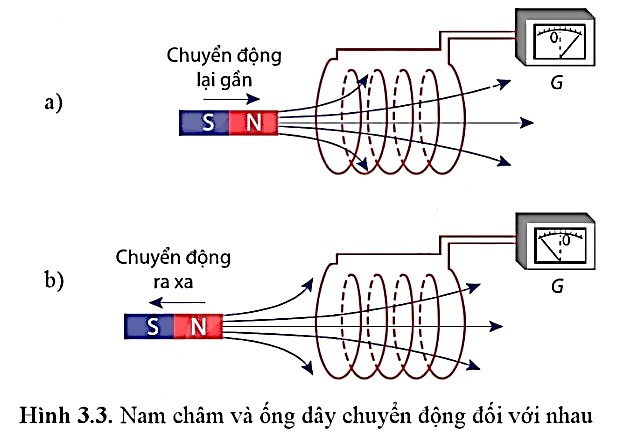
\includegraphics[width=0.4\linewidth]{figs/VN12-Y24-PH-SYL-020P-17}
	\end{center}
	\choice
	{\True có độ lớn tăng lên}
	{có độ lớn giảm đi}
	{có độ lớn không đổi}
	{đảo ngược chiều}
	\loigiai{}
\end{ex}
% ===================================================================
\begin{ex}
	Ví dụ nào sau đây \textbf{không phải} là ví dụ về cảm ứng điện từ?
	\choice
	{Một khung dây quay trong từ trường sẽ tạo ra suất điện động trong khung dây dẫn đó}
	{Một nam châm di chuyển lại gần và ra xa ống dây dẫn sẽ tạo ra một điện áp trong ống dây dẫn đó}
	{\True Một dây dẫn có dòng điện chịu một lực khi được đặt giữa hai cực của một nam châm}
	{Một sự chênh lệch điện thế được tạo ra trên một dây dẫn chuyển động trong từ trường}
	\loigiai{}
\end{ex}
% ===================================================================
\begin{ex}
	Phát biểu nào sau đây nói đến hiện tượng cảm ứng điện từ?
	\choice
	{Sự tạo ra suất điện động qua một dây dẫn khi không có chuyển động giữa dây dẫn và từ trường}
	{Sự tạo ra suất điện động qua một dây dẫn khi có sự chuyển động tương đối giữa dây dẫn và dòng điện cảm ứng}
	{Sự tạo ra suất điện động qua một dây dẫn khi không có chuyển động giữa dây dẫn và dòng điện cảm ứng}
	{\True Sự tạo ra suất điện động qua một dây dẫn khi có chuyển động tương đối giữa dây dẫn và từ trường}
	\loigiai{}
\end{ex}
% ===================================================================
\begin{ex}
	Trong hiện tượng cảm ứng điện từ, suất điện động cảm ứng sinh ra do sự biến thiên của từ thông theo thời gian được xác định bằng biểu thức
	\choice
	{\True $e=-N \frac{\Delta \Phi}{\Delta t}$}
	{$e=N \frac{\Delta \Phi}{\Delta t}$}
	{$e=-N \Delta \Phi \Delta t$}
	{$e=N \Delta \Phi \Delta t$}
	\loigiai{
		
	}
\end{ex}
% ===================================================================
\begin{ex}
	Xét một vòng kim loại đang chuyển động đều từ A đến E như hình \ref{fig:20P-1}. Trong quá trình chuyển động, vòng đi vào vùng từ trường đều abcd có các đường sức từ vuông góc với mặt phẳng vòng dây. Trong quá trình chuyển động, số lượng đường sức từ xuyên qua vòng kim loại này giảm dần trong giai đoạn nào?
	\begin{center}
		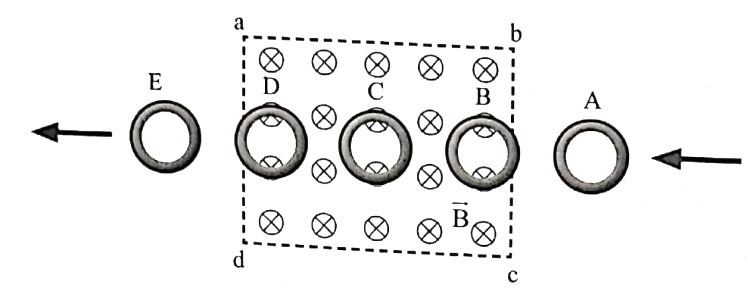
\includegraphics[width=0.4\linewidth]{figs/VN12-Y24-PH-SYL-020P-1}
		\captionof{figure}{}
		\label{fig:20P-1}
	\end{center}
	\choice
	{Từ A đến B}
	{Từ B đến C}
	{Từ C đến D}
	{\True Từ D đến E}
	\loigiai{
		
	}
\end{ex}
% ===================================================================
\begin{ex}
	Khi nam châm dịch chuyển ra xa ống dây, trong ống dây có dòng điện cảm ứng. Nếu nhìn từ phía thanh nam châm vào đầu ống dây, phát biểu nào sau đây là \textbf{đúng}?
	\begin{center}
		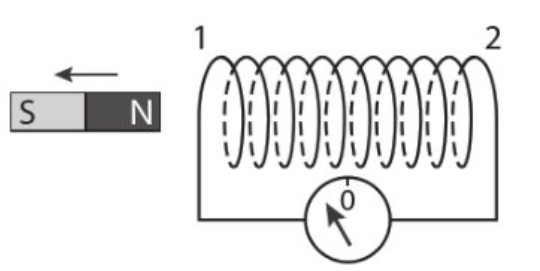
\includegraphics[width=0.4\linewidth]{figs/VN12-Y24-PH-SYL-020P-18}
	\end{center}
	\choice
	{Dòng điện chạy theo chiều kim đồng hồ, đầu 1 là cực bắc của ống dây và hút cực bắc của thanh nam châm}
	{Dòng điện chạy ngược chiều kim đồng hồ, đầu 1 là cực bắc của ống dây và đẩy cực nam của thanh nam châm}
	{Dòng điện chạy ngược chiều kim đồng hồ, đầu 1 là cực nam của ống dây và đẩy cực nam của thanh nam châm}
	{\True Dòng điện chạy theo chiều kim đồng hồ, đầu 1 là cực nam của ống dây và hút cực bắc của thanh nam châm}
	\loigiai{}
\end{ex}

% ===================================================================
\begin{ex}
	Trường hợp nào trong hình bên dưới xác định đúng chiều dòng điện cảm ứng trong vòng dây dẫn kín?
	\choice
	{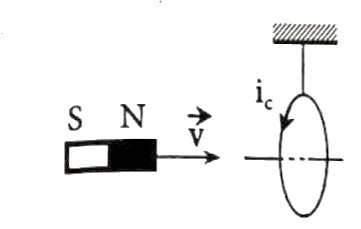
\includegraphics[width=0.42\linewidth]{figs/VN12-Y24-PH-SYL-020P-12a}}
	{\True 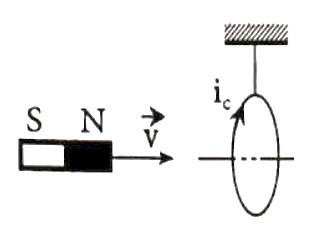
\includegraphics[width=0.42\linewidth]{figs/VN12-Y24-PH-SYL-020P-12b}}
	{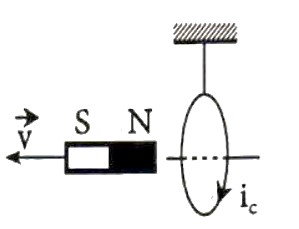
\includegraphics[width=0.42\linewidth]{figs/VN12-Y24-PH-SYL-020P-12c}}
	{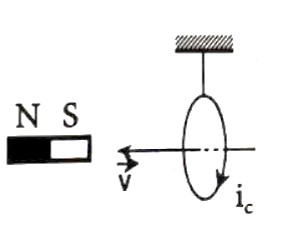
\includegraphics[width=0.42\linewidth]{figs/VN12-Y24-PH-SYL-020P-12d}}
	\loigiai{}
\end{ex}
% ===================================================================
\begin{ex}
	Khi cho nam châm rơi qua vòng dây như hình \ref{fig: 20P-13}.
	\begin{center}
		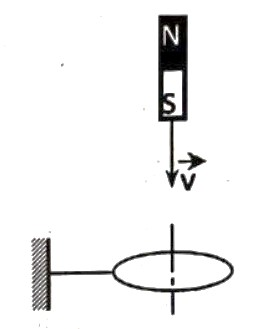
\includegraphics[width=0.2\linewidth]{figs/VN12-Y24-PH-SYL-020P-13}
		\captionof{figure}{}
		\label{fig: 20P-13}
	\end{center}
	Nhận xét nào sau đây là \textbf{đúng} nếu nhìn vòng dây theo hướng từ dưới lên?
	\choice
	{\True Lúc đầu, dòng điện cảm ứng cùng chiều kim đồng hồ. Khi nam châm xuyên qua vòng dây, dòng điện cảm ứng đổi chiều ngược chiều kim đồng hồ}
	{Lúc đầu, dòng điện cảm ứng ngược chiều kim đồng hồ. Khi nam châm xuyên qua vòng dây, dòng điện cảm ứng không đổi chiều}
	{Không có dòng điện cảm ứng trong vòng dây khi nam châm đi vào hoặc đi ra khỏi vòng dây}
	{Dòng điện cảm ứng xuất hiện trong vòng dây luôn cùng chiều kim đồng hồ}
	\loigiai{}
\end{ex}
% ===================================================================
\begin{ex}
	Trường hợp nào trong hình bên dưới mô tả đúng chiều của dòng điện cảm ứng $i_c$ khi cho vòng dây tịnh tiến với vận tốc $\vec{v}$ trong từ trường đều?
	\choice
	{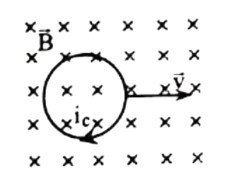
\includegraphics[width=0.4\linewidth]{figs/VN12-Y24-PH-SYL-020P-14a}}
	{\includegraphics[width=0.4\linewidth]{figs/VN12-Y24-PH-SYL-020P-14b}}
	{\includegraphics[width=0.4\linewidth]{figs/VN12-Y24-PH-SYL-020P-14c}}
	{\True \includegraphics[width=0.4\linewidth]{figs/VN12-Y24-PH-SYL-020P-14d}}
	\loigiai{}
\end{ex}

% ===================================================================
\begin{ex}
	Dòng điện cảm ứng $I_c$ trong vòng dây có chiều như hình vẽ, lúc này
	\begin{center}
		\includegraphics[width=0.4\linewidth]{figs/VN12-Y24-PH-SYL-020P-22}
	\end{center}
	\choice
	{từ trường của nam châm đang tăng đều}
	{\True nam châm đang rời xa cuộn dây}
	{nam châm đang đứng yên}
	{nam châm đang đến gần cuộn dây}
	\loigiai{
		Chiều dòng điện $I_c$ cùng chiều kim đồng hồ nên cảm ứng từ $\vec{B}_c$ hướng vào khung dây và cùng chiều $\vec{B}\Rightarrow$ từ thông qua khung khung đang giảm $\rightarrow$ nam châm đang ra xa khung dây.
	} 
\end{ex}
% ===================================================================
\begin{ex}
	Cho P và Q là hai vòng dây dẫn đồng trục đặt cách nhau một khoảng như hình. Khi khoá k đóng, dòng điện chạy cùng chiều kim đồng hồ trong P và có dòng điện cảm ứng $i_{c1}$ chạy trong Q. Sau đó, mở khoá k, có dòng cảm ứng $i_{c2}$ chạy trong Q. Khi đó chiều của $i_{c1}$ và chiều của $i_{c2}$ lần lượt là
	\begin{center}
		\includegraphics[width=0.3\linewidth]{figs/VN12-Y24-PH-SYL-020P-23}
	\end{center}
	\choice
	{cùng chiều và ngược chiều kim đồng hồ}
	{đều cùng chiều kim đồng hồ}
	{đều ngược chiều kim đồng hồ}
	{\True ngược chiều và cùng chiều kim đồng hồ}
	\loigiai{}
\end{ex}
% ===================================================================
\begin{ex}
	Một khung dây gồm 1000 vòng, mỗi vòng có diện tích là $\SI{80}{\centi\meter^2}$. Khung dây được đặt trong từ trường đều sao cho vector cảm ứng từ vuông góc với vector đơn vị pháp tuyến của mặt phẳng vòng dây. Độ lớn cảm ứng từ là $\SI{0.8}{\tesla}$. Quay khung dây quanh trục quay vuông góc với vector cảm ứng từ thì trong khung dây xuất hiện suất điện động cảm ứng trung bình có độ lớn $\SI{6.4}{\volt}$. Sau khoảng thời gian $\SI{1}{\second}$ tính từ lúc khung dây bắt đầu quay, góc hợp bởi vector cảm ứng từ và mặt phẳng khung dây có thể nhận giá trị nào dưới đây?
	\choice
	{\True $\SI{90}{\degree}$}
	{$\SI{0}{\degree}$}
	{$\SI{30}{\degree}$}
	{$\SI{45}{\degree}$}
	\loigiai{
		Từ biểu thức xác định độ lớn suất điện động cảm ứng trung bình, ta có:
		$$
		\begin{aligned}
			& |e|=N\left|\frac{\Delta \Phi}{\Delta t}\right|=N\left|\frac{B S\left(\cos \alpha-\cos \SI{90}{\degree}\right)}{\Delta t}\right| \\
			& \Rightarrow|\cos \alpha|=\frac{|e| \Delta t}{N B S}=\frac{6,4\cdot1}{1000 \cdot 0,8\cdot8 \cdot 10^{-3}}=1, \text { suy ra: } \alpha=k \cdot \SI{180}{\degree}(k=0; \pm 1; \pm 2; \dots) \\
			& \Rightarrow \alpha=\SI{0}{\degree}
		\end{aligned}
		$$
		
		Vậy góc hợp bởi vector cảm ứng từ và mặt phẳng khung dây là $90^{\circ}$.
	}
\end{ex}
% ===================================================================
\begin{ex}
	Một vòng dây kín có diện tích $\SI{50}{\deci\meter^2}$ đặt trong từ trường đều sao cho vector cảm ứng từ song song và cùng chiều với vector đơn vị pháp tuyến của mặt phẳng vòng dây. Độ lớn cảm ứng từ biến thiên theo thời gian như đồ thị trong hình \ref{fig:20P-2}. Độ lớn suất điện động cảm ứng sinh ra trong vòng dây bằng bao nhiêu?
	\begin{center}
		\begin{tikzpicture}  
			\begin{axis}[  ultra thick,
				xmin=0,  
				xmax=0.12,  
				xtick={0,0.05,...,0.10},
				ytick={0,0.1,...,0.5},
				minor x tick num=1,
				minor y tick num=1,
				ymin=0,  
				ymax=0.55, 
				samples=300,
				xticklabel style={/pgf/number format/.cd, fixed,
					fixed zerofill, precision=2},
				axis lines=center, 
				grid style={step=1, line width =0.4pt, color=gray!30!white},
				grid=both, %giới hạn ô lưới
				major grid style={line width=0.8pt,gray!60!white},
				xlabel=$\xsi{t}{\left(\si{\second}\right)}$, 		ylabel=$\xsi{B}{\left(\si{\tesla}\right)}$,
				every axis y label/.style={at=(current axis.above origin),anchor=south},  
				every axis x label/.style={at=(current axis.right of origin),anchor=west},]
				\addplot [ultra thick, blue, smooth, domain=0:0.1] {5*x};  
			\end{axis}  
		\end{tikzpicture}
		\captionof{figure}{}
		\label{fig:20P-2}
	\end{center}
	
	\choice
	{\True $\SI{2.5}{\volt}$}
	{$\SI{-5}{\volt}$}
	{$\SI{-2.5}{\volt}$}
	{$\SI{5}{\volt}$}
	\loigiai{
		$$
		\begin{aligned}
			&\text { Độ lớn suất điện động cảm ứng sinh ra trong vòng dây là: }\\
			&|e|=\left|\frac{\Delta \Phi}{\Delta t}\right|=\left|\frac{S\Delta B}{\Delta t}\right|=\left|\frac{0,5 \cdot 0,5}{0,1}\right|=\SI{2.5}{\volt}
		\end{aligned}
		$$
	}
\end{ex}
% ===================================================================
\begin{ex}
	Một khung dây dẫn kín hình vuông có cạnh dài $\SI{10}{\centi\meter}$ gồm 500 vòng được đặt trong từ trường đều sao cho vector đơn vị pháp tuyến của mặt phẳng khung dây cùng phương cùng chiều với vector cảm ứng từ. Điện trở suất và tiết diện của dây kim loại có giá trị lần lượt là $\SI{2E-8}{\ohm\cdot\meter}$ và $\SI{0.4}{\milli\meter^2}$. Giá trị cảm ứng từ biến thiên theo thời gian như đồ thị trong hình \ref{fig:20P-3}. Công suất toả nhiệt sinh ra trong khung dây có giá trị bao nhiêu?
	\begin{center}
		\begin{tikzpicture}  
			\begin{axis}[  ultra thick,
				xmin=0,  
				xmax=0.12,  
				xtick={0,0.05,...,0.10},
				ytick={0,0.1,...,0.5},
				minor x tick num=1,
				minor y tick num=1,
				ymin=0,  
				ymax=0.55, 
				samples=300,
				xticklabel style={/pgf/number format/.cd, fixed,
					fixed zerofill, precision=2},
				axis lines=center, 
				grid style={step=1, line width =0.4pt, color=gray!30!white},
				grid=both, %giới hạn ô lưới
				major grid style={line width=0.8pt,gray!60!white},
				xlabel=$\xsi{t}{\left(\si{\second}\right)}$, 		ylabel=$\xsi{B}{\left(\si{\tesla}\right)}$,
				every axis y label/.style={at=(current axis.above origin),anchor=south},  
				every axis x label/.style={at=(current axis.right of origin),anchor=west},]
				\addplot [ultra thick, blue, smooth, domain=0:0.1] {0.5-3*x};  
			\end{axis}  
		\end{tikzpicture}
		\captionof{figure}{}
		\label{fig:20P-3}
	\end{center}
	\choice
	{$\SI{225}{\milli\watt}$}
	{\True $\SI{22.5}{\watt}$}
	{$\SI{0.09}{\milli\watt}$}
	{$\SI{9}{\watt}$}
	\loigiai{
		Độ lớn suất điện động cảm ứng sinh ra trong khung dây là:
		$$
		|e|=N\left|\frac{\Delta \Phi}{\Delta t}\right|=N S\left|\frac{\Delta B}{\Delta t}\right|=500\cdot0,1^2 \cdot\left|\frac{0,2-0,5}{0,1}\right|=\SI{15}{\volt}
		$$
		Gọi tiết diện của dây kim loại là $S^{\prime}$. Điện trở của dây kim loại trong khung dây là:
		$$
		R=\rho \frac{\ell}{S^{\prime}}=2 \cdot 10^{-8} \cdot \frac{500 \cdot 0,1 \cdot 4}{0,4 \cdot 10^{-6}}=\SI{10}{\ohm}.
		$$
		Công suất toả nhiệt trong khung dây: $\calP=\frac{|e|^2}{R}=\frac{15^2}{10}=\SI{22.5}{\watt}$.
	}
\end{ex}

% ===================================================================
\begin{ex}
	Một khung dây dẫn kín có 500 vòng được đặt trong từ trường đều có độ lớn cảm ứng từ là $\SI{0.4}{\tesla}$. Diện tích mỗi vòng dây là $\SI{50}{\centi\meter^2}$. Cho khung dây quay đều quanh trục vuông góc với vector cảm ứng từ với tốc độ góc là $\xsi{\dfrac{\pi}{3}}{\radian/\second}$. Nối khung dây với tụ điện thì tụ điện tích được một lượng điện tích là $\SI{3}{\micro\coulomb}$. Giả sử điện trở của khung dây là không đáng kể và ban đầu vector cảm ứng từ cùng phương, cùng chiều với vector đơn vị pháp tuyến của mặt phẳng khung dây. Điện dung của tụ điện có giá trị là 
	\choice
	{$\SI{3}{\farad}$}
	{$\SI{3}{\micro\farad}$}
	{$\SI{6}{\farad}$}
	{\True $\SI{6}{\micro\farad}$}
	\loigiai{
		Khung dây quay đều quanh trục vuông góc với vector cảm ứng từ với tốc độ góc là $\xsi{\frac{\pi}{3}}{\radian/\second}$, nghĩa là trong $\SI{1}{\second}$ khung dây quay được một góc là $\xsi{\dfrac{\pi}{3}}{\radian}$.\\
		Độ lớn suất điện động cảm ứng trung bình sinh ra trong khung dây có giá trị là:
		$$
		\begin{aligned}
			|e|=N\left|\frac{\Delta \Phi}{\Delta t}\right|&=N\left|\frac{B S[\cos (\alpha+\omega t)-\cos \alpha]}{\Delta t}\right| \\
			& =500\left|\frac{0,4 \cdot 5 \cdot 10^{-3}\left(\cos \frac{\pi}{3}-\cos 0\right)}{1}\right|=\SI{0.5}{\volt}
		\end{aligned}
		$$
		Vì khung dây có điện trở không đáng kể nên $|e|=U$. Từ công thức tính điện tích của tụ điện, suy ra:
		$$
		Q=C U \Rightarrow C=\frac{Q}{U}=\frac{3}{0,5}=\SI{6}{\micro\farad}.
		$$
	}
\end{ex}

% ===================================================================
\begin{ex}
	Trường hợp nào trong hình bên dưới xác định đúng chiều dòng điện cảm ứng trong khung dây dẫn?
	\choice
	{\True \includegraphics[width=0.4\linewidth]{figs/VN12-Y24-PH-SYL-020P-15a}}
	{\includegraphics[width=0.4\linewidth]{figs/VN12-Y24-PH-SYL-020P-15b}}
	{\includegraphics[width=0.4\linewidth]{figs/VN12-Y24-PH-SYL-020P-15c}}
	{\includegraphics[width=0.4\linewidth]{figs/VN12-Y24-PH-SYL-020P-15d}}
	\loigiai{}
\end{ex}

\Closesolutionfile{ans}
\subsubsection{Trắc nghiệm đúng/sai}
\Opensolutionfile{ans}[ans/VN12-Y24-PH-SYL-020P-TF]
\setcounter{ex}{0}
% ===================================================================
\begin{ex}
	Nối hai đầu cuộn dây dẫn kín với điện kế và cho chuyển động rơi tự do qua một nam châm như hình \ref{fig: 20P-10}. Biết cảm ứng từ, đường sức từ của nam châm được mô tả như hình vẽ và khi bắt đầu chuyển động, kim điện kế chỉ vạch số 0.
	\begin{center}
		\includegraphics[width=0.2\linewidth]{figs/VN12-Y24-PH-SYL-020P-10}
		\captionof{figure}{}
		\label{fig: 20P-10}
	\end{center}
	Các nhận định sau đây là đúng hay sai?
	\choiceTF[t]
	{Cuộn dây rơi tự do nên kim điện kế không bị lệch khỏi vạch số 0 khi đi qua đầu trên của nam châm}
	{Thời điểm cuộn dây rơi đến giữa nam châm thì kim điện kế bị lệch xa nhất khỏi vạch số 0}
	{Thời điểm cuộn dây rơi ra khỏi đầu dưới của nam châm thì kim điện kế chỉ vạch số 0}
	{Chiều dòng điện cảm ứng xuất hiện tại thời điểm cuộn dây đi vào nam châm và cuộn dây đi ra khỏi nam châm là như nhau}
	\loigiai{
		
	}
\end{ex}
% ===================================================================
\begin{ex}
	Đặt hai cuộn dây dẫn kín cạnh nhau, như hình \ref{fig: 20P-11}. Một cuộn nối với nguồn điện. Một cuộn nối với điện kế, khi không có dòng điện chạy trong cuộn dây thì kim điện kế chỉ vạch số 0.
	\begin{center}
		\includegraphics[width=0.3\linewidth]{figs/VN12-Y24-PH-SYL-020P-11}
		\captionof{figure}{}
		\label{fig: 20P-11}
	\end{center}
	Các nhận định sau đây là đúng hay sai?
	\choiceTF[t]
	{\True Kim điện kế bị lệch khỏi vạch số 0 khi nguồn điện là nguồn xoay chiều}
	{Kim điện kế bị lệch khỏi vạch số 0 khi nguồn điện là nguồn điện một chiều}
	{Mắc cuộn dây với nguồn điện một chiều và dịch chuyển cuộn dây ra xa thì kim điện kế không bị lệch khỏi vạch số 0}
	{\True Mắc cuộn dây (1) với nguồn một chiều và dùng tay bóp bẹp cuộn dây 2 thì kim điện kế sẽ bị lệch khỏi vạch số 0}
	\loigiai{}
\end{ex}
% ===================================================================
\begin{ex}
	Một cuộn dây đồng gồm nhiều vòng đặt gần một nam châm thẳng.
	\begin{center}
		\includegraphics[width=0.3\linewidth]{figs/VN12-Y24-PH-SYL-020P-24}
	\end{center}
	Cuộn dây được di chuyển theo hướng mũi tên thể hiện trong sơ đồ.
	\choiceTF[t]
	{Dòng điện cảm ứng trong cuộn dây chạy từ B đến A}
	{Nếu đổi cực nam châm thì trong cuộn dây sẽ không có dòng điện cảm ứng}
	{\True Khi di chuyển cuộn dây nhanh lên thì dòng điện trong cuộn dây sẽ tăng lên}
	{Nếu cho cuộn dây và nam châm di chuyển cùng chiều với cùng tốc độ thì dòng điện cảm ứng trong cuộn dây là dòng điện không đổi}
	\loigiai{
		\begin{itemchoice}
			\itemch Sai. Di chuyển cuộn dây lại gần nam châm thì từ thông qua cuộn dây tăng nên dòng điện cảm ứng trong cuộn dây có chiều sao cho từ trường do nó sinh ra ngược chiều từ trường của nam châm. Do $\vec{B}$ của nam châm hướng sang trái nên $\vec{B}_c$ do dòng điện cảm ứng trong cuộn dây sinh ra hướng sang phải $\Rightarrow$ Mặt B của cuộn dây là mặt Bắc và mặt A của cuộn dây là mặt Nam $\rightarrow$ Dòng điện cảm ứng cùng chiều kim đồng hồ nhìn từ mặt A nên chạy từ A đến B.
			\itemch Sai. Khi đổi cực nam châm và cuộn dây di chuyển lại gần nam châm thì từ thông qua cuộn dây vẫn biến thiên và sinh ra dòng điện cảm ứng.
			\itemch Đúng. Khi di chuyển cuộn dây nhanh lên thì tốc độ biến thiên từ thông qua cuộn dây sẽ tăng lên $\rightarrow$ dòng điện trong cuộn dây sẽ tăng lên.
			\itemch Sai. Lúc này không có sự biến thiên từ thông qua cuộn dây nên không có dòng điện cảm ứng.
			
		\end{itemchoice}	
	}
\end{ex}
% ===================================================================
\begin{ex}
	Một cuộn dây được nối với vôn kế, một nam châm được giữ phía trên cuộn dây.
	\begin{center}
		\includegraphics[width=0.3\linewidth]{figs/VN12-Y24-PH-SYL-021-8}
	\end{center}	
	\choiceTF[t]
	{\True Khi thả cho nam châm rơi vào cuộn dây, kim vôn kế bị lệch}
	{Nếu nam châm được thả từ độ cao lớn hơn, số chỉ cực đại trên vôn kế vẫn như khi nam châm được thả từ độ cao thấp hơn}
	{Khi cuộn dây có nhiều vòng dây hơn, số chỉ trên vôn kế sẽ giảm}
	{Nếu cực Nam của nam châm đi vào cuộn dây trước, kim chỉ trên vôn kế vẫn lệch như khi cực Bắc của nam châm rơi vào cuộn dây trước}
	\loigiai{
		\begin{itemchoice}
			\itemch Đúng. Khi nam châm rơi, từ thông qua cuộn dây thay đổi, sinh ra dòng điện cảm ứng. Sự thay đổi này gây ra suất điện động cảm ứng làm kim vôn kế lệch.
			\itemch Sai. Khi nam châm rơi từ độ cao lớn hơn, nó sẽ tăng tốc khi đi qua cuộn dây do đó tốc độ thay đổi từ thông tăng lên làm tăng số chỉ cực đại trên vôn kế.
			\itemch Sai. Cuộn dây có nhiều vòng dây hơn sẽ tạo ra suất điện động cảm ứng lớn hơn khi nam châm di chuyển qua, dẫn đến số chỉ trên vôn kế sẽ tăng.
			\itemch Sai. Số chỉ trên vôn kế sẽ ngược lại.
			
		\end{itemchoice}	
	}
\end{ex}

% ===================================================================
\begin{ex}
	Một khung kim loại hình tròn đường kính $\SI{5}{\centi\meter}$ được đặt trong vùng từ trường đều có các đường sức từ vuông góc với mặt phẳng khung dây. Hai đầu của khung dây được nối với một bóng đèn nhỏ tạo thành mạch kín. Lấy $\pi \approx 3,14$; biết điện trở của khung kim loại và bóng đèn lần lượt là $R_1=\SI{2}{\ohm}$ và $R_2=\SI{1}{\ohm}$. Tại thời điểm ban đầu $(t=\SI{0}{\second})$, người ta bắt đầu thay đổi độ lớn cảm ứng từ theo đồ thị như hình \ref{fig:20P-4}. Trong mỗi phát biểu sau, em hãy chọn đúng hoặc sai.	
	\begin{center}
		\begin{tikzpicture}  
			\begin{axis}[  ultra thick,
				xmin=0,  
				xmax=6,  
				xtick={0,1,...,5},
				ytick={0,150,...,500},
				minor x tick num=0,
				minor y tick num=0,
				ymin=0,  
				ymax=600, 
				samples=300,
				axis lines=center, 
				grid style={step=1, line width =0.4pt, color=gray!30!white},
				grid=both, %giới hạn ô lưới
				major grid style={line width=0.8pt,gray!60!white, dashed},
				xlabel=$\xsi{t}{\left(\si{\second}\right)}$, 		ylabel=$\xsi{B}{\left(\si{\milli\tesla}\right)}$,
				every axis y label/.style={at=(current axis.above origin),anchor=south},  
				every axis x label/.style={at=(current axis.right of origin),anchor=west},  ]
				\draw[line width =0.8pt, color=gray!60!white, dashed] (axis cs: 0,500)--(axis cs: 6,500);
				\addplot [ultra thick, blue, smooth, domain=0:1] {150*x};  
				\addplot [ultra thick, blue, smooth, domain=1:3] {150}; 
				\addplot [ultra thick, blue, smooth, domain=3:4] {150+350*(x-3)};
				\addplot [ultra thick, blue, smooth, domain=4:5] {500-500*(x-4)}; 
			\end{axis}  
			\node[left] at (-0.1,4.8) {500};
		\end{tikzpicture}
		\captionof{figure}{}
		\label{fig:20P-4}
	\end{center}
	
	\choiceTFt
	{\True Tại thời điểm $t=\SI{0}{\second}$, không có từ thông xuyên qua khung kim loại}
	{\True Tổng thời gian đèn sáng trong quá trình thay đổi nói trên là $\SI{3}{\second}$}
	{Mặc dù dòng điện cảm ứng chạy qua đèn trong khoảng thời gian từ $t=\SI{3}{\second}$ đến $t=\SI{4}{\second}$ và từ $t=\SI{4}{\second}$ đến $t=\SI{5}{\second}$ ngược chiều nhau nhưng cường độ dòng điện có cùng độ lớn}
	{Suất điện động cảm ứng sinh ra trong khoảng thời gian từ $t=\SI{0}{\second}$ đến $t=\SI{1}{\second}$ là $\SI{1.1775E-3}{\volt}$}
	{Độ sáng của đèn trong khoảng thời gian từ $t=\SI{0}{\second}$ đến $t=\SI{1}{\second}$ mạnh hơn trong khoảng thời gian từ $t=\SI{3}{\second}$ đến $t=\SI{4}{\second}$}
	{\True Nhiệt lượng toả ra trên bóng đèn trong một giây cuối cùng của quá trình thay đổi độ lớn cảm ứng từ xấp xỉ $\SI{1.1E-7}{\joule}$}
	\loigiai{
	}
\end{ex}
\Closesolutionfile{ans}
\subsubsection{Tự luận}
\setcounter{ex}{0}
\Opensolutionfile{ans}[ans/VN12-Y24-PH-SYL-020P-TL]
% ======================================================================
\begin{ex}
	Đoạn dây dẫn ở hình \ref{fig:20P-19} là một phần của mạch điện kín. Khi nâng đoạn dây dẫn thẳng đứng lên trên, trong đoạn dây xuất hiện dòng điện cảm ứng. Dòng điện cảm ứng trong đoạn dây dẫn sẽ thay đổi thế nào khi
	\begin{center}
		\includegraphics[width=0.2\linewidth]{figs/VN12-Y24-PH-SYL-020P-19}
		\captionof{figure}{}
		\label{fig:20P-19}
	\end{center}
	\begin{enumerate}[label=\alph*)]
		\item Di chuyển đoạn dây dẫn thẳng đứng xuống dưới?
		\item Giữ đoạn dây dẫn nằm yên?
		\item Di chuyển đoạn dây dẫn song song với đường sức từ?
	\end{enumerate}
	
	\loigiai{
		\begin{enumerate}[label=\alph*)]
			\item Dòng điện đảo chiều.
			\item Không có dòng điện cảm ứng.
			\item Không có dòng điện cảm ứng.
		\end{enumerate}	
	}
\end{ex}
% ======================================================================
\begin{ex}
	Giải thích vì sao thời gian quay của một đĩa nhôm giữa hai cực từ của một nam châm lại nhỏ hơn khi không có nam châm?
	\loigiai{
		Dòng điện xoáy sinh ra trong đĩa tạo ra từ trường cản trở chuyển động.	
	}
\end{ex}

% ======================================================================
\begin{ex}
	Cho một khung kim loại gồm 1000 vòng dây có diện tích $\SI{25}{\centi\meter^2}$ quay quanh trục trong một từ trường đều với độ lớn cảm ứng từ là $\SI{0.01}{\tesla}$ như hình \ref{fig:20P-5}a. Hình \ref{fig:20P-5}b biểu diễn vị trí của khung tại một số thời điểm khác nhau trong quá trình quay so với vector cảm ứng từ. Giá trị góc $\alpha$ hợp bởi vector cảm ứng từ $\vec{B}$ và vector đơn vị pháp tuyến của mặt phẳng khung dây $\vec{n}$ tại một số thời điểm được ghi lại trong bảng bên dưới. Hãy xác định giá trị của từ thông tương ứng với các trường hợp được liệt kê trong hình \ref{fig:20P-4}.
	\begin{center}
		\includegraphics[width=0.9\linewidth]{figs/VN12-Y24-PH-SYL-020P-5}
		\captionof{figure}{}
		\label{fig:20P-5}
	\end{center}
	\begin{center}
		\begin{tabular}{|M{2.5cm}|M{1.25cm}|M{1.25cm}|M{1.25cm}|M{1.25cm}|M{1.25cm}|M{1.25cm}|M{1.25cm}|M{1.25cm}|M{1.25cm}|}
			\hline
			\thead{Thời điểm}&(1)& (2)&(3)&(4)& (5)& (6)& (7)&(8)&(9)\\
			\hline
			$\alpha$&$\SI{0}{\degree}$&$\SI{45}{\degree}$&$\SI{90}{\degree}$&$\SI{135}{\degree}$&$\SI{180}{\degree}$&$\SI{135}{\degree}$&$\SI{90}{\degree}$&$\SI{45}{\degree}$&$\SI{0}{\degree}$\\
			\hline
			$\xsi{\Phi}{\left(\weber\right)}$&&&&&&&&&\\
			\hline
		\end{tabular}
	\end{center}
	\loigiai{
		Áp dụng công thức $\Phi=NBS\cos\alpha$, ta được các giá trị của từ thông trong bảng sau:
		\begin{center}
			\begin{tabular}{|M{2.5cm}|M{1.25cm}|M{1.25cm}|M{1.25cm}|M{1.25cm}|M{1.25cm}|M{1.25cm}|M{1.25cm}|M{1.25cm}|M{1.25cm}|}
				\hline
				\thead{Thời điểm}&(1)& (2)&(3)&(4)& (5)& (6)& (7)&(8)&(9)\\
				\hline
				$\alpha$&$\SI{0}{\degree}$&$\SI{45}{\degree}$&$\SI{90}{\degree}$&$\SI{135}{\degree}$&$\SI{180}{\degree}$&$\SI{135}{\degree}$&$\SI{90}{\degree}$&$\SI{45}{\degree}$&$\SI{0}{\degree}$\\
				\hline
				$\xsi{\Phi}{\left(\weber\right)}$&0,025&$\dfrac{\sqrt{2}}{80}$&0&$-\dfrac{\sqrt{2}}{80}$&$-0,025$&$-\dfrac{\sqrt{2}}{80}$&0&$\dfrac{\sqrt{2}}{80}$&0,025\\
				\hline
			\end{tabular}
		\end{center}
	}
\end{ex}
% ======================================================================
\begin{ex}
	Xét một sóng điện từ đang lan truyền trong không gian với thành phần điện trường tại một điểm A biến thiên điều hoà theo phương trình $E=1,5 \sin (120 t+\pi)\ \left(\si{\volt/\meter}\right)$.
	\begin{enumerate}[label=\alph*)]
		\item Hãy xác định tần số góc và pha ban đầu trong sự biến thiên của thành phần từ trường tại điểm A.
		\item Tại thời điểm $t$, cường độ điện trường tại A có giá trị $\SI{1.5}{\volt/\meter}$. Sau khoảng thời gian bằng một phần tư chu kì thì cảm ứng từ tại điểm đó có giá trị bằng bao nhiêu?	
	\end{enumerate}
	\loigiai{
		\begin{enumerate}[label=\alph*)]
			\item Vì cả hai thành phần điện trường và từ trường trong sóng điện từ biến thiên cùng tần số, cùng pha với nhau nên tần số góc và pha ban đầu cần tìm lần lượt là $\omega=\SI{120}{\radian/\second}$ và $\varphi=\xsi{\pi}{\radian}$.
			\item Ta thấy tại thời điểm $t$ cuờng độ điện trường đang đạt giá trị cực đại, suy ra thành phần từ trường cũng đạt giá trị cực đại. Do đó, sau một phần tư chu kì truyền sóng thì giá trị của cảm ứng từ tại điểm đó sẽ bằng không.
		\end{enumerate}
	}
\end{ex}
% ======================================================================
\begin{ex}
	Cho một thanh kim loại ab đang được kéo đều trên đường ray dẫn điện. Cả hệ thống đường ray và thanh ab đang được đặt trong vùng từ trường đều có hướng vuông góc với mặt phẳng khung và có chiều như hình \ref{fig:20P-6}. Trong quá trình thanh di chuyển, từ trường sinh ra bởi dòng điện cảm ứng có chiều hướng như thế nào? Vì sao?
	\begin{center}
		\includegraphics[width=0.4\linewidth]{figs/VN12-Y24-PH-SYL-020P-6}
		\captionof{figure}{}
		\label{fig:20P-6}
	\end{center}
	\loigiai{
		Khi thanh kim loại ab chuyển động sang phải, diện tích giới hạn bởi đường ray và thanh kim loại tăng lên làm cho từ thông tăng dần. Theo định luật Lenz về hiện tượng cảm ứng điện từ, dòng điện cảm ứng sinh ra có chiều chống lại nguyên nhân sinh ra nó, tức là từ trường sinh ra bởi dòng điện này phải có tác dụng làm giảm sự tăng lên của từ thông. Chính vì vậy các đường sức từ của từ trường do dòng điện cảm ứng sinh ra hướng ngược lại với các đường sức từ ban đầu.
	}
\end{ex}
% ======================================================================
\begin{ex}
	Một dây dẫn bằng sắt được uốn thành vòng tròn và đang được đặt trong vùng từ trường đều với các đường sức từ hướng vuông góc với mặt phẳng vòng dây như hình \ref{fig:20P-8}. Hãy mô tả chiều của dòng điện cảm ứng sinh ra trong các trường hợp dưới đây:
	\begin{center}
		\begin{tikzpicture}
			\foreach \x in {0,0.75,...,3.75}{
				\foreach \y in {0,0.75,...,3.75}{
					\node[blue] at (\x, \y) {\LARGE$\odot$};
				}
			}
			\node[blue, right] at(3,3.25) {$\vec{B}$};
			\draw[line width=1.5pt] (1.875,1.875) circle (1.5);
		\end{tikzpicture}
		\captionof{figure}{}
		\label{fig:20P-8}
	\end{center}
	\begin{enumerate}[label=\alph*)]
		\item Trường hợp 1: Độ lớn cảm ứng từ được điều chỉnh giảm dần theo thời gian.
		\item Trường hợp 2: Độ lớn cảm ứng từ được điều chỉnh tăng dần theo thời gian.
		\item Trường hợp 3: Từ vị trí ban đầu, tịnh tiến vòng kim loại sang trái (vòng kim loại vẫn nằm trong vùng từ trường).
	\end{enumerate}
	\loigiai{
		\begin{enumerate}[label=\alph*)]
			\item Sự giảm dần của độ lớn cảm ứng từ dẫn đến số đường sức từ xuyên qua mặt phẳng vòng dây giảm dần, do đó từ thông qua vòng dây giảm và trong vòng dây xuất hiện dòng điện cảm ứng. Từ trường sinh ra bởi dòng điện cảm ứng sẽ hướng vuông góc với mặt phẳng vòng kim loại và hướng ra khỏi mặt giấy (theo định luật Lenz về hiện tượng cảm ứng điện từ). Dựa vào quy tắc nắm tay phải, dòng điện cảm ứng sẽ hướng ngược chiều kim đồng hồ.	
			\item Lập luận tương tự như câu a, ta thấy lúc này dòng điện cảm ứng hướng cùng chiều kim đồng hồ.
			\item Vì từ thông xuyên qua vòng dây không đổi theo thời gian nên không có dòng điện cảm ứng xuất hiện trong vòng kim loại.
		\end{enumerate}
	}
\end{ex}
% ======================================================================
\begin{ex}
	Một hình vuông cạnh $\SI{5}{\centi\meter}$ đặt trong từ trường đều có cảm ứng từ $B=\SI{8E-4}{\tesla}$. Từ thông qua hình vuông đó bằng $\SI{E-6}{\weber}$. Tính góc hợp bởi vector cảm ứng từ với mặt phẳng của hình vuông đó.
	\loigiai{
		Diện tích khung dây: $S=\SI{25E-4}{\meter^2}$.\\
		Áp dụng công thức tính từ thông: $\Phi=BS \cos \alpha \Rightarrow \cos \alpha=\frac{1}{2} \Rightarrow \alpha= \pm \xsi{\frac{\pi}{3}}{\radian}$. \\
		Trong đó $\alpha$ là góc tạo bởi vector pháp tuyến của mặt phẳng hình vuông và vector cảm ứng từ, nên góc tạo bởi vector cảm ứng từ với mặt phẳng hình vuông là: $\beta=\dfrac{\pi}{2}-\alpha=\xsi{\dfrac{\pi}{6}}{\radian}$ hoặc $\xsi{\dfrac{5 \pi}{6}}{\radian}$.\\
		Do góc hợp bởi vector cảm ứng từ với mặt phẳng của hình vuông là góc nhọn, nên chọn $\beta=\xsi{\dfrac{\pi}{6}}{\radian}$.
	}
\end{ex}
% ======================================================================
\begin{ex}
	Một khung dây dẫn gồm 200 vòng có diện tích $\SI{8.5}{\centi\meter^2}$ và mặt phẳng khung dây vuông góc với cảm ứng từ có độ lớn thay đổi từ $\SI{0.03}{\tesla}$ đến $\SI{0.12}{\tesla}$ trong $\SI{15}{\milli\second}$. Tính độ lớn suất điện động cảm ứng trong khung dây.
	\loigiai{
		Độ lớn suất điện động cảm ứng:
		$$\left|e\right|=\left|\dfrac{NS\Delta B}{\Delta t}\right|=\SI{1.02}{\volt}.$$	
	}
\end{ex}
% ======================================================================
\begin{ex}
	Một vòng dây dẫn phẳng hình tròn có diện tích $S=\SI{30}{\centi\meter^2}$ ở trong một từ trường dều có $B=\SI{0.2}{\tesla}$. Trong $\SI{0.5}{\second}$ vòng dây quay đều được một góc $\SI{60}{\degree}$. Tìm:
	\begin{center}
		\includegraphics[width=0.3\linewidth]{figs/VN12-Y24-PH-SYL-020P-21}
	\end{center}
	\begin{enumerate}[label=\alph*)]
		\item độ lớn suất điện động cảm ứng trong vòng dây.
		\item chiều của dòng điện cảm ứng trong vòng dây.
	\end{enumerate}
	\loigiai{
		\begin{enumerate}[label=\alph*)]
			\item $\SI{6E-4}{\volt}$
			\item dòng điện có hướng ngược chiều kim đồng hồ (nhìn từ trên xuống vòng dây).
		\end{enumerate}	
	}
\end{ex}
% ======================================================================
\begin{ex}
	Một khung dây kín có 100 vòng, mỗi vòng có diện tích là $\SI{80}{\deci\meter^2}$. Vòng dây được đặt trong từ trường đều sao cho vector cảm ứng từ hợp với vector đơn vị pháp tuyến của mặt phẳng khung dây một góc $\alpha$. Độ lớn cảm ứng từ biến thiên theo thời gian như đồ thị trong hình \ref{fig:20P-7}. Độ lớn suất điện động cảm ứng trong vòng dây có giá trị là $\SI{40}{\volt}$. Góc $\alpha$ có giá trị là bao nhiêu?
	\begin{center}
		\begin{tikzpicture}  
			\begin{axis}[  ultra thick,
				xmin=0,  
				xmax=1.1,  
				xtick={0,0.2,...,1},
				ytick={0,0.4,...,2.4},
				minor x tick num=1,
				minor y tick num=1,
				ymin=0,  
				ymax=2.6, 
				samples=300,
				yticklabel style={/pgf/number format/.cd, fixed,
					fixed zerofill, precision=1},
				axis lines=center, 
				grid style={step=1, line width =0.4pt, color=gray!30!white},
				grid=both, %giới hạn ô lưới
				major grid style={line width=0.8pt,gray!60!white},
				xlabel=$\xsi{t}{\left(\si{\second}\right)}$, 		ylabel=$\xsi{B}{\left(\si{\tesla}\right)}$,
				every axis y label/.style={at=(current axis.above origin),anchor=south},  
				every axis x label/.style={at=(current axis.right of origin),anchor=west},  ]
				\addplot [ultra thick, blue, smooth, domain=0:6] {0.4+2*x}; 
			\end{axis}  
		\end{tikzpicture}
		\captionof{figure}{}
		\label{fig:20P-7}
	\end{center}
	
	\loigiai{
		Từ biểu thức tính độ lớn suất điện động cảm ứng, ta suy ra giá trị của góc hợp bởi vector cảm ứng từ và vector đơn vị pháp tuyến của mặt phẳng khung dây như sau:
		$$
		\begin{aligned}
			& \left|e\right|=N\left|\frac{\Delta \Phi}{\Delta t}\right|=N \frac{|\Delta B| S \cos \alpha}{\Delta t} \\
			\Rightarrow & \cos \alpha=\frac{|e| \Delta t}{N|\Delta B| S}=\frac{40\cdot1}{100\cdot2 \cdot 0,8}=0,25 \Rightarrow \alpha \approx \SI{75.5}{\degree}
		\end{aligned}
		$$
	}
\end{ex}
% ======================================================================
\begin{ex}
	Một nhóm học sinh dùng ống dây nối với điện kế nhạy có điểm 0 ở giữa để làm thí nghiệm về hiện tượng cảm ứng diện từ. Họ di chuyển một thanh nam châm lại gần một đầu ống dây như hình \ref{fig: 20P-20}. Kim của điện kế lệch sang trái.
	\begin{center}
		\includegraphics[width=0.3\linewidth]{figs/VN12-Y24-PH-SYL-020P-20}
		\captionof{figure}{}
		\label{fig: 20P-20}
	\end{center}
	\begin{enumerate}[label=\alph*)]
		\item Giải thích tại sao kim của điện kế di chuyển.
		\item Hãy đề xuất cách làm cho kim điện kế lệch sang phải.
		\item Nêu cách làm thế nào để có được số chỉ lớn hơn trên điện kế.
		\item Cho biết số chỉ của điện kế sẽ thế nào nếu giữ nam châm đứng yên trong ống dây.
	\end{enumerate}
	\loigiai{
		\begin{enumerate}[label=\alph*)]
			\item Ống dây và từ trường đang chuyển động tương đối với nhau, do đó xuất hiện một suất điện động cảm ứng trong ống dây.
			\item Di chuyển nam châm ra khỏi ống dây hoặc di chuyển ống dây ra khỏi nam châm hoặc đưa cực nam của nam châm vào cùng một đầu của ống dây hoặc đưa cực bắc của nam châm vào đầu kia của ống dây.
			\item Di chuyển nam châm nhanh hơn hoặc sử dụng nam châm mạnh hơn hoặc tăng số vòng trên một đơn vị chiều dài của ống dây.
			\item Kim chỉ số 0.
		\end{enumerate}	
	}
\end{ex}
% ======================================================================
\begin{ex}
	Một cuộn dây dẫn kín, dẹt hình tròn, gồm $\mathrm{N}=100$ vòng, mỗi vòng có bán kính $r=\SI{10}{\centi\meter}$, mỗi mét chiều dài của dây dẫn có điện trở $R_0=\SI{0.5}{\ohm}$. Cuộn dây đặt trong một từ trường đều có vector cảm ứng từ $\vec{B}$ vuông góc với mặt phẳng các vòng dây và có độ lớn $B=\SI{E-2}{\tesla}$ giảm đều đến 0 trong thời gian $\Delta t=\SI{E-2}{\second}$. Tính cường độ dòng điện cảm ứng xuất hiện trong cuộn dây.
	\loigiai{
		Từ thông qua một vòng dây của cuộn dây là: $\Phi=B S \cos \alpha$, trong đó $\alpha=0$ và $S=\pi r^2$. Xét trong khoảng thời gian từ $t_0=0$ đến thời điểm $t$, từ thông qua 1 vòng dây thay đổi từ $\Phi_0$ đến $\Phi_1$ ứng với cảm ứng từ là $B_0=\SI{E-2}{\tesla}$ và $B_t=0$.\\
		Theo định luật Faraday ta có suất điện động cảm ứng qua $N$ vòng dây của cuộn dây là:
		$$
		e=-N \frac{\Delta\Phi}{\Delta t}=-NS \frac{\Delta B}{\Delta t}
		$$\\
		Cường độ dòng điện cảm ứng xuất hiện trong cuộn dây là: $i=\dfrac{e}{R}$\\
		Trong đó, $R=LR_0=N2 \pi rR_0$ là điện trở của khung dây.\\
		Do đó, $i=-N \pi r^2 \dfrac{\dfrac{\Delta B}{\Delta t}}{N 2 \pi rR_0}=-\dfrac{r}{2R_0} \cdot \dfrac{\Delta B}{\Delta t}=-\dfrac{0,1}{2 \cdot 0,5} \cdot \dfrac{0-10^{-2}}{10^{-2}}=\SI{0.1}{\ampere}$.
		
	}
\end{ex}
% ======================================================================
\begin{ex}
	Một khung dây dẫn hình vuông, cạnh $a=\SI{10}{\centi\meter}$, đặt cố định trong từ trường đều có vector cảm ứng từ $\vec{B}$ vuông góc với mặt phẳng khung. Trong khoảng thời gian $\Delta t=\SI{0.05}{\second}$, cho độ lớn của $B$ tăng đều từ 0 đến $\SI{0.5}{\tesla}$. Xác định độ lớn của suất điện động cảm ứng xuất hiện trong khung.
	\loigiai{
		Ta có $\alpha=0$ và $N=1$,\\
		nên $\left|e\right|=\left|-N\dfrac{\Delta \Phi}{\Delta t}\right|=\left|-S\dfrac{\Delta B}{\Delta t}\right|=\left|-0,1^2\cdot\dfrac{0,5}{0,05}\right|=\SI{0.1}{\volt}=\SI{100}{\milli\volt}.$
	}
\end{ex}
% ======================================================================
\begin{ex}
	Để giám sát quá trình hô hấp của bệnh nhân, các nhân viên y tế sử dụng một đai mỏng gồm 250 vòng dây kim loại quấn liên tiếp nhau được buộc xung quanh ngực của bệnh nhân như hình \ref{fig:20P-9}. Khi bệnh nhân hít vào, diện tích của các vòng dây tăng lên một lượng $\SI{45}{\centi\meter^2}$. Biết từ trường Trái Đất tại vị trí đang xét được xem gần đúng là đều và có độ lớn cảm ứng từ xấp xỉ $\SI{56}{\micro\tesla}$, các đường sức từ hợp với mặt phẳng cuộn dây một góc $\SI{32}{\degree}$. Giả sử thời gian để một bệnh nhân hít vào là $\SI{1.5}{\second}$, hãy xác định độ lớn suất điện động cảm ứng trung bình sinh ra bởi cuộn dây trong quá trình nói trên.
	\begin{center}
		\includegraphics[width=0.4\linewidth]{figs/VN12-Y24-PH-SYL-020P-9}
		\captionof{figure}{}
		\label{fig:20P-9}
	\end{center}
	
	\loigiai{
		Độ lớn suất điện động cảm ứng trung bình sinh ra trong quá trình hít vào là:
		$$
		\left|e\right|=N\left|\frac{\Delta \Phi}{\Delta t}\right|=N\left|\frac{B \Delta S \cos \alpha}{\Delta t}\right|=\left|\frac{250 \cdot 56 \cdot 10^{-6} \cdot 45 \cdot 10^{-4} \cdot \cos \left(\SI{90}{\degree}-\SI{32}{\degree}\right)}{1,5}\right| \approx \SI{2.2E-5}{\volt}.
		$$
	}
\end{ex}

% ======================================================================
\begin{ex}
	Một khung dây cứng, phẳng diện tích $\SI{25}{\centi\meter^2}$, gồm 10 vòng dây. Khung dây được đặt trong từ trường đều. Khung dây nằm trong mặt phẳng như hình \ref{fig: 20P-16}. Cảm ứng từ biến thiên theo thời gian như đồ thị.
	\begin{center}
		\includegraphics[width=0.4\linewidth]{figs/VN12-Y24-PH-SYL-020P-16}
		\captionof{figure}{}
		\label{fig: 20P-16}
	\end{center}
	\begin{enumerate}[label=\alph*)]
		\item Tính độ biến thiên của từ thông qua khung dây kể từ lúc $t=0$ đến $t=\SI{0.4}{\second}$.
		\item Xác định suất điện động cảm ứng trong khung.
		\item Tìm chiều của dòng điện cảm ứng trong khung.
	\end{enumerate}
	\loigiai{
		\begin{enumerate}[label=\alph*)]
			\item Tại thời điếm $t_0=0$ thì $B_0=\SI{2.4E-3}{\tesla}$; thời điểm $t=\SI{0.4}{\second}$ thì $B_t=\SI{0}{\tesla}$ và góc $\alpha=0$.\\
			Do đó, ta có $\Delta \Phi=\Phi_1-\Phi_0=NS\cdot \Delta B=10 \cdot 25 \cdot 10^{-4} \cdot\left(-2,4 \cdot 10^{-3}\right)=\SI{-6E-5}{\weber}$.
			\item Theo định luật Faraday ta có: 
			$$e=-\frac{\Delta \Phi}{\Delta t}=\frac{6 \cdot 10^{-5}}{0,4}=\SI{1.5E-4}{\volt}=\SI{0.15}{\milli\volt}.$$
			\item Cảm ứng từ $B$ giảm nên theo định luật Lenz cảm ứng từ do dòng điện cảm ứng sinh ra sẽ cùng chiều với cảm ứng từ $B$. Theo quy tắc bàn tay phải, tìm được chiều dòng điện cảm ứng theo chiều kim đồng hồ chạy trong cuộn dây.
		\end{enumerate}
	}
\end{ex}
% ======================================================================
\begin{ex}
	Một khung dây kín phẳng hình vuông ABCD có cạnh $a=\SI{10}{\centi\meter}$ gồm $N=250$ vòng. Khung chuyển động thẳng đều tiến lại khoảng không gian có từ trường đều. Trong khi chuyển động, cạnh AB và DC luôn nằm trên hai đường thẳng song song như hình \ref{fig: 20P-17}. 
	\begin{center}
		\begin{tikzpicture}
			\coordinate (A) at (-1.5,-1.5);
			\coordinate (B) at (1.5,-1.5);
			\coordinate (C) at (1.5,1.5);
			\coordinate (D) at (-1.5,1.5);
			\coordinate (A') at (3,-2);
			\coordinate (B') at (7,-2);
			\coordinate (C') at (7,2);
			\coordinate (D') at (3,2);
			\foreach \i in {3.5,4.5,5.5,6.5}{
				\foreach \j in {-1.5,-0.5,0.5,1.5}{
					\node[blue] at (\i, \j) {\LARGE $\otimes$};
				}
			};
			\draw[line width=1.5pt] (A)--(B)--(C)--(D)--(A);
			\draw[line width=1pt, dashed] (A')--(B')--(C')--(D')--(A');
			\draw[-stealth, line width=1.5pt, red] (1.5,0)--(2.5,0);
			\node[below] at(A) {A};
			\node[below] at(B) {B};
			\node[above] at(C) {C};
			\node[above] at(D) {D};
			\node[below] at(A') {A'};
			\node[below] at(B') {B'};
			\node[above] at(C') {C'};
			\node[above] at(D') {D'};
			\node[above, red] at (2.5,0) {$\vec{v}$};
		\end{tikzpicture}
		\captionof{figure}{}
		\label{fig: 20P-17}
	\end{center}
	Tính cường độ dòng điện cảm ứng chạy trong khung trong khoảng thời gian từ khi cạnh CB của khung bắt đầu gặp từ trường đến khi khung vừa vặn nằm hẳn trong từ trường. Chỉ rõ chiều dòng điện trong khung. Cho biết điện trở của khung là $\SI{3}{\ohm}$. Tốc độ của khung $v=\SI{1.5}{\meter/\second}$ và cảm ứng từ của từ trường $B=\SI{0.005}{\tesla}$.
	\loigiai{
		Tại thời điểm $t_0=0$ khi khung dây có cạnh BC bắt đầu vào vùng từ trường đếu thì diện tích khung dây nằm trong từ trường $S_0=0$ và thời điểm t thì diện tích khung dây vào trong từ trường là $S_t=BC\cdot vt= avt$ và góc $\alpha=0 \Rightarrow$ từ thông qua 1 vòng của khung dây là $\Phi_t=BS_t=Bav\cdot\Delta t$\\
		Theo định luật Faraday ta có:
		$$
		e=-N \dfrac{\Delta \Phi}{\Delta t}=N \dfrac{Bav \cdot \Delta t}{\Delta t}=NBav=250\cdot 0,005 \cdot 0,1 \cdot 1,5=\SI{0.1875}{\volt}.
		$$
		
		Lại có $$i=\dfrac{e}{R}=\dfrac{NBav}{R}=\dfrac{0,1875}{3}=\SI{0.0625}{\ampere}=\SI{62.5}{\milli\ampere}.$$
		Khi khung dây đi vào vùng từ trường, từ thông qua khung dây tăng, nên cảm ứng từ do dòng điện cảm ứng sinh ra ngược chiều với cảm ứng từ của vùng từ trường, do đó, chiều dòng điện qua khung theo chiều ngược chiều kim đồng hồ hay có chiều từ A đến B .
	}
\end{ex}
% ======================================================================
\begin{ex}
	Một khung dây hình chữ nhật có các cạnh lần lượt là: $a=\SI{10}{\centi\meter}$; $b=\SI{20}{\centi\meter}$ gồm 50 vòng dây quay đều trong một từ trường đều có cảm ứng từ $B=\SI{0.5}{\tesla}$. Trục quay của khung nằm vuông góc với đường sức từ. Lúc đầu, mặt phẳng khung vuông góc với vector cảm ứng từ. Khung quay với tốc độ góc $\omega=\xsi{100\pi}{\radian/\second}$. Tính suất điện động cảm ứng trung bình trong khung dây trong thời gian nó quay được $\SI{15}{\degree}$ kể từ vị trí ban đầu.
	\loigiai{
		Tại thời điểm $t_0=0: \alpha=0$; tại thời điểm $t: \alpha=\omega t=\xsi{\dfrac{\pi}{12}}{\radian}$ nên $t=\xsi{\dfrac{1}{12} \cdot 10^{-2}}{\second}\Rightarrow$ từ thông qua mỗi vòng dây là: $\Phi=BS \cos \alpha$.\\
		Theo định luật Faraday ta có:
		$$
		e=-N \dfrac{\Delta \Phi}{\Delta t}=-NBS \dfrac{\cos \dfrac{\pi}{12}-\cos 0}{\Delta t}=-50\cdot0,5 \cdot 0,1 \cdot 0,2 \dfrac{\cos \dfrac{\pi}{12}-\cos 0}{\dfrac{1}{12} \cdot 10^{-2}}=\SI{20.44}{\volt}.
		$$
	}
\end{ex}
\Closesolutionfile{ans}\newpage
%	\section{Chuyển động của đoạn dây dẫn mang dòng điện trong từ trường}
\subsection{Tóm tắt lí thuyết}
\begin{tomtat}
	Một đoạn dây MN có chiều dài $\ell$ được đặt trên hai thanh kim loại và tạo thành một mạch kín. Tất cả được đặt trong một từ trường đều có cảm ứng từ $\vec{B}$.
	\begin{center}
		\includegraphics[width=0.4\linewidth]{figs/VN12-Y24-PH-SYL-022-1}
	\end{center}
	Khi đoạn dây dẫn chuyển động với tốc độ $\vec{v}$, suất điện động cảm ứng trong đoạn dây:
	\begin{equation}
		\left|e_c\right|=\left|\dfrac{\Delta \Phi}{\Delta t}\right|
	\end{equation}
	\begin{itemize}
		\item Khi $\vec{v}$ và $\vec{B}$ cùng vuông góc với đoạn dây chuyển động, đồng thời $\vec{v}$ vuông góc với $\vec{B}$ thì
		$$\Delta \Phi=B\Delta S=B\ell v\Delta t$$
		Như vậy:
		\begin{equation}
			\left|e_c\right|=B\ell v
		\end{equation}
		\item Nếu $\vec{v}$ và $\vec{B}$ cùng vuông góc với đoạn dây chuyển động, nhưng $\vec{v}$ tạo với $\vec{B}$ một góc $\theta$ thì:
		\begin{equation}
			\left|e_c\right|=B\ell v\sin\theta
		\end{equation}
	\end{itemize}
	\begin{noidung}{Quy tắc bàn tay phải để xác định chiều dòng điện cảm ứng trong đoạn dây chuyển động trong từ trường đều}
		Đặt bàn tay phải hứng các đường sức từ, ngón tay cái choãi ra $\SI{90}{\degree}$ hướng theo chiều chuyển động của đoạn dây, khi đó đoạn dây dẫn đóng vai trò như một nguồn điện, chiều từ cổ tay đến các ngón tay còn lại chỉ chiều dòng điện cảm ứng trên đoạn dây.
	\end{noidung}
\end{tomtat}
\subsection{Ví dụ minh hoạ}
\begin{dang}{Xác định suất điện động cảm ứng trong một đoạn dây dẫn chuyển động}
	\end{dang}
\begin{vd}
Thanh kim loại AB dài $\SI{20}{\centi\meter}$ kéo trượt đều trên hai thanh ray kim loại nằm ngang như hình vẽ. Các dây nối nhau bằng điện trở $R=\SI{3}{\ohm}$. Vận tốc của thanh AB là $\SI{12}{\meter/\second}$. Hệ thống đặt trong từ trường đều có $B=\SI{0.4}{\tesla}$, $\vec{B}$ vuông góc với mạch điện.
\begin{center}
	\begin{tikzpicture}
		\coordinate (O) at (0,0);
		\coordinate (A) at (2,1.5);
		\coordinate (B) at (2,-1.5);
		\coordinate (C) at (-4,0);
		\draw[line width=1.5pt] (A)--++(-6,0)--++(0,-3)--(B);
		\node[draw, rectangle, line width=1.5pt, fill=white, minimum height=2cm, minimum width=0.5cm, anchor=center] at (C){};
		\draw[blue, line width=1.5pt, -stealth] (O)--+(2,0);
		\draw[line width=5pt] (O)--+(0,2)--+(0,-2);
		\node[right] at ($(C)+(0.25,0)$) {$R$};
		\node[red] at ($(O)!0.5!(C)$) {\LARGE$\otimes$};
		\node[red, below] at ($(O)!0.5!(C)-(0,0.25)$) {$\vec{B}$};
		\node[blue, above] at ($(O)+(2,0)$) {$\vec{v}$};
		\node[above right] at ($(O)+(0,1.5)$) {B};
		\node[below right] at ($(O)-(0,1.5)$) {A};
	\end{tikzpicture}
\end{center}
\begin{enumerate}[label=\alph*)]
	\item Tính độ lớn suất điện động cảm ứng xuất hiện trong khung.
	\item Xác định chiều và tính cường độ dòng điện cảm ứng chạy qua đoạn mạch.
\end{enumerate}	
\loigiai{\begin{enumerate}[label=\alph*)]
		\item Độ lớn suất điện động cảm ứng trong thanh:
		$$\left|e_c\right|=B\ell v\sin\theta=\left(\SI{0.4}{\tesla}\right)\cdot\left(\SI{0.2}{\meter}\right)\cdot\left(\SI{12}{\meter/\second}\right)\cdot\sin\SI{90}{\degree}=\SI{0.96}{\volt}.$$
		\item Cường độ dòng điện cảm ứng trong mạch:
		$$i_c=\dfrac{\left|e_c\right|}{R}=\SI{0.32}{\ampere}.$$
		Áp dụng quy tắc bàn tay phải suy ra chiều của dòng điện cảm ứng đi qua thanh AB có chiều từ A đến B.
\end{enumerate}}
\end{vd}
% =========================================
\begin{vd}
	Cho mạch điện có sơ đồ như hình vẽ, nguồn điện có suất điện động $\calE=\SI{1.5}{\volt}$, điện trở trong $r=\SI{0.1}{\ohm}$, thanh MN có chiều dài $\SI{1}{\meter}$ và có điện trở $R=\SI{2.9}{\ohm}$. Từ trường $\vec{B}$ có phương vuông góc với mặt phẳng khung và hướng vào trong khung như hình vẽ, có độ lớn $B=\SI{0.1}{\tesla}$. Thanh MN có điện trở không đáng kể.
	\begin{center}
		\begin{tikzpicture}
			\coordinate (O) at (0,0);
			\coordinate (A) at (2,1.5);
			\coordinate (B) at (2,-1.5);
			\coordinate (C) at (-2,1.5);
			\coordinate (D) at (-4,0);
			\draw[line width=1.5pt] (A)--++(-6,0)--++(0,-3)--(B);
			\node[draw,line width=1.5pt, shape=circle, radius=2.5cm, fill=orange!15!white, anchor=center] at (C){\color{red}A};
			\node[draw,line width=1.5pt,white, rectangle,fill=white,minimum height=0.2cm,minimum width=1.5cm, anchor=center] at (D){};
			\draw[line width=1.5pt] ($(D)+(0,0.1)$)--+(0.5,0)--+(-0.5,0);
			\draw[line width=2.5pt] ($(D)-(0,0.1)$)--+(0.25,0)--+(-0.25,0);
			\draw[blue, line width=1.5pt, -stealth] (O)--+(2,0);
			\draw[line width=5pt] (O)--+(0,2)--+(0,-2);
			\node[red] at ($(C)-(0,1.5)$) {\LARGE$\otimes$};
			\node[red, below] at ($(C)-(0,1.65)$) {$\vec{B}$};
			\node[blue, above] at ($(O)+(2,0)$) {$\vec{v}$};
			\node[above right] at ($(O)+(0,1.5)$) {N};
			\node[below right] at ($(O)-(0,1.5)$) {M};
			\node[left] at ($(D)-(0.5,0)$) {$\calE, r$};
		\end{tikzpicture}
	\end{center}
	\begin{enumerate}[label=\alph*)]
		\item Ampere kế chỉ bao nhiêu khi MN đứng yên? Tính độ lớn lực từ tác dụng lên thanh MN khi đó.
		\item Ampere kế chỉ bao nhiêu khi MN di chuyển về phía phải với tốc độ $v=\SI{3}{\meter/\second}$ sao cho hai đầu MN luôn tiếp xúc với hai thanh đỡ bằng kim loại? Tính độ lớn lực từ tác dụng lên thanh MN khi đó.
		\item Muốn ampere kế chỉ số $0$ phải để thanh MN di chuyển về phía nào, với vận tốc là bao nhiêu?
	\end{enumerate}
	\loigiai{\begin{enumerate}[label=\alph*)]
			\item Khi thanh MN đứng yên thì trong mạch không có dòng điện cảm ứng nên số chỉ ampere kế là
			$$I=\dfrac{\calE}{R+r}=\dfrac{\SI{1.5}{\volt}}{\SI{3}{\ohm}}=\SI{0.5}{\ampere}.$$
			Độ lớn lực từ tác dụng lên thanh MN:
			$$F=I\ell B=\left(\SI{0.5}{\ampere}\right)\cdot\left(\SI{1}{\meter}\right)\cdot\left(\SI{0.1}{\tesla}\right)=\SI{0.05}{\newton}.$$
			\item Khi thanh MN chuyển động về phía phải thì trong mạch xuất hiện dòng điện cảm ứng có chiều từ M đến N và có độ lớn:
			$$i_c=\dfrac{e_c}{R+r}=\dfrac{B\ell v}{R+r}=\dfrac{\left(\SI{0.1}{\tesla}\right)\cdot\left(\SI{1}{\meter}\right)\cdot\left(\SI{3}{\meter/\second}\right)}{\SI{3}{\ohm}}=\SI{0.1}{\ampere}.$$
			Do $i_c$ ngược chiều với dòng điện do nguồn tạo ra nên cường độ dòng điện qua ampere kế:
			$$I_A=I-i_c=\SI{0.4}{\ampere}.$$
			Lực từ tác dụng lên thanh MN:
			$$F=I_A\ell B=\SI{0.04}{\newton}.$$
			\item Muốn ampere kế chỉ số 0 thì $i_c$ phải có độ lớn bằng $I=\SI{0.5}{\ampere}$ và ngược chiều với $I$. Như vậy, thanh MN phải di chuyển từ trái sang phải.\\
			Tốc độ chuyển động của thanh MN lúc này:
			$$i_c=\dfrac{B\ell v'}{R+r}\Rightarrow v'=\dfrac{i_c\left(R+r\right)}{B\ell}=\SI{15}{\meter/\second}.$$
	\end{enumerate}	}
\end{vd}

\begin{dang}{Chuyển động của đoạn dây dẫn mang dòng điện trong từ trường đều}
	\end{dang}
\begin{vd}
	Hai thanh kim loại song song, thẳng đứng có điện trở không đáng kể, một đầu nối vào điện trở $R=\SI{0.5}{\ohm}$. Một đoạn dây dẫn AB, độ dài $\ell=\SI{14}{\centi\meter}$, khối lượng $m=\SI{2}{\gram}$, điện trở $r=\SI{0.5}{\ohm}$ tì vào hai thanh kim loại. Ban đầu người ta giữ cố định dây AB rồi thả cho nó tự do trượt không ma sát xuống dưới và luôn vuông góc với hai thanh kim loại. Toàn bộ hệ thống đặt trong từ trường đều có hướng vuông góc với mặt phẳng hai thanh kim loại có cảm ứng từ $B=\SI{0.2}{\tesla}$. Lấy $g=\SI{9.8}{\meter/\second^2}$.
	\begin{center}
		\begin{tikzpicture}
			\coordinate (A) at (0,0);
			\coordinate (B) at (4,0);
			\draw[line width=1.5pt] (0,-2)--++(0,4)--++(4,0)--++(0,-4);
			\node[draw, rectangle,fill=white, line width=1.5pt, minimum height=0.4cm, minimum width=1.5cm] at (2,2) {};
			% Thanh AB
			\draw[line width=4pt] (-0.5,0)--(4.5,0);
			
			\node[below] at(2,1.8) {$R$};
			\node[below left] at(A) {A};
			\node[below right] at(B) {B};
			\node[red] at (2,1) {\LARGE$\odot$};
			\node[red,below] at (2,0.8) {$\vec{B}$};
		\end{tikzpicture}
	\end{center}
	\begin{enumerate}[label=\alph*)]
		\item Xác định chiều dòng điện qua điện trở $R$.
		\item Chứng minh rằng lúc đầu thanh AB chuyển động nhanh dần, sau một thời gian chuyển động thì thanh AB chuyển động thẳng đều. Tính tốc độ chuyển động thẳng đều ấy và tính hiệu điện thế giữa hai đầu A, B.
		\item Bây giờ đặt hai thanh kim loại nghiêng với mặt phẳng nằm ngang một góc $\alpha=\SI{60}{\degree}$. Độ lớn và chiều của $\vec{B}$ vẫn như cũ. Tính tốc độ $v$ của chuyển động đều của thanh AB và $U_\text{AB}$.
	\end{enumerate}
	\loigiai{
	\begin{enumerate}[label=\alph*)]
		\item Do thanh đi xuống nên từ thông qua mạch tăng. Áp dụng định luật Lenz, dòng điện cảm ứng sinh ra $\vec{B}_c$ ngược chiều $\vec{B}$.\\
		Áp dụng quy tắc nắm bàn tay phải, $i_c$ có chiều từ B đến A.
		\begin{center}
			\begin{tikzpicture}
				\coordinate (A) at (0,0);
				\coordinate (B) at (4,0);
				\draw[line width=1.5pt, decoration={markings, mark=at position 0.4 with {\arrow{stealth}}},
				postaction={decorate}] (0,-2)--++(0,4)--++(4,0)--++(0,-4);
				\node[draw, rectangle,fill=white, line width=1.5pt, minimum height=0.4cm, minimum width=1.5cm] at (2,2) {};
				% Thanh AB
				\draw[line width=4pt
				] (4.5,0)--(-0.5,0);
				
				\node[below] at(2,1.8) {$R$};
				\node[below left] at(A) {A};
				\node[below right] at(B) {B};
				\node[red] at (3,1) {\LARGE$\odot$};
				\node[red,below] at (3,0.8) {$\vec{B}$};
				\node[blue] at (1,1) {\LARGE$\otimes$};
				\node[blue,below] at (1,0.8) {$\vec{B}_c$};
				\node[above left, blue] at(1,2) {$i_c$};
			\end{tikzpicture}
		\end{center}
		\item Ngay sau khi buông, thanh AB chỉ chịu tác dụng của trọng lực $\vec{P}=m\vec{g}$ nên thanh chuyển động nhanh dần $\rightarrow v$ tăng dần.\\
		Đồng thời, trong mạch xuất hiện dòng điện cảm ứng $i_c$ nên thanh AB chịu thêm tác dụng của lực từ $F=i_c\ell B$ có hướng đi lên.\\
		Mặt khác, suất điện động cảm ứng xuất hiện bên rong AB là $e_c=B\ell v$ nên
		$$i_c=\dfrac{e_c}{R+r}=\dfrac{B\ell v}{R+r}\Rightarrow F=\dfrac{B^2\ell^2v}{R+r}.$$
		Cho nên khi $v$ tăng dần thì $F$ tăng dần $\rightarrow$ tồn tại thời điểm mà $F=P$. Khi đó, thanh chuyển động thẳng đều.\\
		Khi thanh chuyển động đều thì:
		$$F=mg\Rightarrow \dfrac{B^2\ell^2v}{R+r}=mg\Rightarrow v=\dfrac{\left(R+r\right)mg}{B^2\ell^2}=\SI{25}{\meter/\second}.$$
		Hiệu điện thế giữa hai đầu thanh AB khi đó:
		$$U_\text{AB}=i_cR=\dfrac{B\ell v}{R+r}\cdot R=\SI{0.35}{\volt}.$$
		\item Khi để nghiêng hai thanh kim loại, ta có:
		\begin{center}
			\begin{tikzpicture}
				\coordinate (O) at (0,0);
				\coordinate (A) at ($(O)+(60:2.5)+(150:0.2)$);
				\coordinate (B) at ($(O)+(60:4)$);
				\coordinate (C) at ($(O)+(0:4)$);
				\coordinate (D) at (4,1.5);
				\draw[line width=1.5pt] (O)--(B);
				\draw[line width=1.5pt] (O)--(C);
				\tkzMarkAngle[size=0.75cm,color=blue, line width=1.5pt](C,O,B);
				\tkzLabelAngle[color=blue,pos=1.0](C,O,B){$\alpha$}
				
				\draw[line width=1.5pt, purple, dashed] ($(D)+(-120:1)$)--($(D)+(-2,0)$);
				\draw[line width=1.5pt, purple, dashed] ($(D)+(150:1.732)$)--($(D)+(-2,0)$);
				\draw[line width=1.5pt, purple, -stealth] (D)--+(-2,0);
				\draw[line width=1.5pt, purple, -stealth] (D)--+(150:1.732);
				\draw[line width=1.5pt, purple, -stealth] (D)--+(-120:1);
				\node[left, purple] at ($(D)+(-2,0)$)  {$\vec{B}$};
				\node[right, purple] at ($(D)+(-120:1)$)  {$\vec{B}_2$};
				\node[above, purple] at ($(D)+(150:1.732)$)  {$\vec{B}_1$};
				% Lực
				\draw[line width=2pt, red, -stealth] (A)--+(0,-2);
				\draw[line width=2pt, green!75!black, -stealth] (A)--+(60:1.5);
				\draw[line width=2pt, black, -stealth] (A)--+(150:1.5);
				\node[black, circle, fill=white, inner sep=0pt, minimum size=0pt] at (A) {\LARGE$\otimes$};
				\node[right,red] at ($(A)+(0,-2)$) {$\vec{P}$};
				\node[above,green!75!black] at ($(A)+(60:1.5)$) {$\vec{F}$};
				\node[above,black] at ($(A)+(150:1.5)$) {$\vec{N}$};
			\end{tikzpicture}
		\end{center}
		Thanh chuyển động đều khi:
		$$F=mg\sin\alpha\Rightarrow \dfrac{\left(B\sin\alpha\right)^2\ell^2v}{R+r}=mg\sin\alpha $$
		$$\Rightarrow v=\dfrac{\left(R+r\right)mg\sin\alpha}{\left(B\sin\alpha\right)^2\ell^2}=\dfrac{\left(\SI{0.5}{\ohm}+\SI{0.5}{\ohm}\right)\cdot\left(\SI{2E-3}{\kilogram}\right)\cdot\left(\SI{9.8}{\meter/\second^2}\right)\cdot\sin\SI{60}{\degree}}{\left[\left(\SI{0.2}{\tesla}\right)\sin\SI{60}{\degree}\right]^2\cdot\left(\SI{0.14}{\meter}\right)^2}=\SI{28.87}{\meter/\second}.$$
	\end{enumerate}	
	Hiệu điện thế giữa hai đầu thanh khi đó là
	$$U_\text{AB}=IR=\dfrac{B\ell v\sin\alpha}{R+r}\cdot R=\dfrac{\left(\SI{0.2}{\tesla}\right)\cdot\left(\SI{0.14}{\meter}\right)\cdot\left(\SI{28.87}{\meter/\second}\right)\sin\SI{60}{\degree}}{\SI{0.5}{\ohm}+\SI{0.5}{\ohm}}\cdot\left(\SI{0.5}{\ohm}\right)=\SI{0.35}{\volt}.$$
	}
\end{vd}
\subsubsection{Trắc nghiệm nhiều phương án lựa chọn}
\setcounter{ex}{0}
\Opensolutionfile{ans}[ans/VN12-Y24-PH-SYL-021P-TN]
% ===================================================================
\begin{ex}
	Chọn phương án đúng về chiều dòng điện cảm ứng trong thanh MN.
	\begin{center}
		\includegraphics[width=0.4\linewidth]{figs/VN12-Y24-PH-SYL-022P-1}
	\end{center}
	\choice
	{Hình a - dòng điện cảm ứng có chiều từ N đến M, hình b - dòng điện cảm ứng có chiều từ N đến M}
	{Hình a - dòng điện cảm ứng có chiều từ M đến N, hình b - dòng điện cảm ứng có chiều từ M đến N}
	{\True Hình a - dòng điện cảm ứng có chiều từ M đến N, hình b - dòng điện cảm ứng có chiều từ N đến M}
	{Hình a - dòng điện cảm ứng có chiều từ N đến M, hình b - dòng điện cảm ứng có chiều từ M đến N}
	\loigiai{}
\end{ex}
% ===================================================================
\begin{ex}
	Đặt khung dây ABCD cạnh một dây dẫn thẳng có dòng điện trên cùng một mặt phẳng như hình
	\begin{center}
		\includegraphics[width=0.25\linewidth]{figs/VN12-Y24-PH-SYL-022P-3}
	\end{center}
	Thanh AB có thể trượt trên thanh DE và CF. Điện trở $R$ không đổi và bỏ qua điện trở của các thanh. Cho AB song song với dòng điện thẳng và chuyển động thẳng đều với tốc độ không đổi. Dòng điện cảm ứng trong mạch có chiều
	\choice
	{từ  A đến B}
	{\True từ B đến A}
	{thay đổi liên tục}
	{không có dòng điện cảm ứng trong mạch}
	\loigiai{}
\end{ex}
% ===================================================================
\begin{ex}
	Đặt khung dây dẫn ABCD trong từ trường đều có chiều như hình vẽ
	\begin{center}
		\includegraphics[width=0.25\linewidth]{figs/VN12-Y24-PH-SYL-022P-4}
	\end{center}
	Thanh AB có thể trượt. Điện trở $R$ không đổi và bỏ qua điện trở các thanh. Cường độ dòng điện cảm ứng trong mạch có biểu thức
	\choice
	{$i=\dfrac{B\ell}{vR}$}
	{$i=B\ell v$}
	{$i=\dfrac{Bv}{\ell R}$}
	{\True $i=\dfrac{B\ell v}{R}$}
	\loigiai{}
\end{ex}


% ===================================================================
\begin{ex}
	Một thanh dẫn điện dài $\SI{80}{\centi\meter}$, chuyển động trong từ trường đều với vận tốc $\SI{2}{\meter/\second}$ và vuông góc với $\vec{B}$. Biết độ lớn cảm ứng từ $B=\SI{0.4}{\tesla}$. Suất điện động cảm ứng trong thanh có độ lớn là	
	\choice
	{\True $\SI{0.64}{\volt}$}
	{$\SI{64}{\volt}$}
	{$\SI{32}{\volt}$}
	{$\SI{0.32}{\volt}$}
	\loigiai{
		Độ lớn suất điện động cảm ứng trong thanh:
		$$\left|e_c\right|=B\ell v\sin\theta=\left(\SI{0.4}{\tesla}\right)\cdot\left(\SI{0.8}{\meter}\right)\cdot\left(\SI{2}{\meter/\second}\right)\cdot\SI{90}{\degree}=\SI{0.64}{\volt}.$$	
	}
\end{ex}

% ===================================================================
\begin{ex}
	Một máy bay có chiều dài cánh $\ell=\SI{68}{\meter}$ bay theo phương ngang với vận tốc $v=\SI{720}{\kilo\meter/\hour}$. Biết thành phần thẳng đứng của cảm ứng từ Trái Đất $B=\SI{5E-5}{\tesla}$. Hiệu điện thế xuất hiện ở hai đầu cánh là
	\begin{center}
		\includegraphics[width=0.3\linewidth]{figs/VN12-Y24-PH-SYL-022P-2}
	\end{center}
	\choice
	{$\SI{2.448}{\volt}$}
	{\True $\SI{0.68}{\volt}$}
	{$\SI{1.224}{\volt}$}
	{$\SI{1.36}{\volt}$}
	\loigiai{
		Hiệu điện thế xuất hiện ở hai cánh máy bay:
		$$U=B\ell v\sin\SI{90}{\degree}=\SI{0.68}{\volt}.$$	
	}
\end{ex}


% ===================================================================
\begin{ex}
	Một thanh dẫn điện dài $\SI{1}{\meter}$, chuyển động trong từ trường đều có cảm ứng từ $B=\SI{0.4}{\tesla}$ với vận tốc $\SI{2}{\meter/\second}$ và hợp với $\vec{B}$ một góc $\SI{30}{\degree}$. Suất điện động cảm ứng trong thanh có độ lớn là
	\choice
	{$\SI{0.4}{\volt}$}
	{$\SI{0.2}{\volt}$}
	{$\SI{0.7}{\volt}$}
	{$\SI{0.8}{\volt}$}
	\loigiai{
		Suất điện động cảm ứng suất hiện trong thanh là
		$$\left|e_c\right|=B\ell v\sin\theta=\left(\SI{0.4}{\tesla}\right)\cdot\left(\SI{1}{\meter}\right)\cdot\left(\SI{2}{\meter/\second}\right)\cdot
		\sin\SI{30}{\degree}=\SI{0.4}{\volt}.$$
	}
\end{ex}
% ===================================================================
\begin{ex}
	Một thanh dẫn điện dài $\SI{1}{\meter}$, chuyển động trong từ trường đều có cảm ứng từ $B=\SI{0.4}{\tesla}$ với vận tốc $\SI{2}{\meter/\second}$ và hợp với $\vec{B}$ một góc $\SI{30}{\degree}$. Dùng dây có điện trở không đáng kể nối hai đầu thanh với một điện trở $R=\SI{2}{\ohm}$ thành một mạch kín. Cường độ dòng điện cảm ứng qua điện trở là
	\choice
	{$\xsi{0.4\sqrt{3}}{\ampere}$}
	{$\xsi{0.2\sqrt{3}}{\ampere}$}
	{$\SI{0.4}{\ampere}$}
	{\True $\SI{0.2}{\ampere}$}
	\loigiai{
		Suất điện động cảm ứng suất hiện trong thanh là
		$$\left|e_c\right|=B\ell v\sin\theta=\left(\SI{0.4}{\tesla}\right)\cdot\left(\SI{1}{\meter}\right)\cdot\left(\SI{2}{\meter/\second}\right)\cdot
		\sin\SI{30}{\degree}=\SI{0.4}{\volt}.$$
		Cường độ dòng điện qua điện trở:
		$$I=\dfrac{\left|e_c\right|}{R}=\SI{0.2}{\ampere}.$$
	}
\end{ex}
% ===================================================================
\begin{ex}
	Thanh kim loại AB dài $\SI{20}{\centi\meter}$ kéo trượt đều trên hai thanh ray kim loại nằm ngang như hình vẽ
	\begin{center}
		\includegraphics[width=0.25\linewidth]{figs/VN12-Y24-PH-SYL-022P-5}
	\end{center}
	Các dây nối với nhau bằng điện trở $R=\SI{3}{\ohm}$, vận tốc của thanh AB là $\SI{12}{\meter/\second}$. Hệ thống đặt trong từ trường đều có $\vec{B}$ vuông góc với mạch điện và có độ lớn cảm ứng từ $B=\SI{0.4}{\tesla}$. Chiều và độ lớn của dòng điện cảm ứng qua thanh AB là
	\choice
	{Chiều từ B đến A, $i_c=\SI{0.32}{\ampere}$}
	{\True Chiều từ A đến B, $i_c=\SI{0.32}{\ampere}$}
	{Chiều từ A đến B, $i_c=\SI{0.96}{\ampere}$}
	{Chiều từ B đến A, $i_c=\SI{0.96}{\ampere}$}
	\loigiai{
		Áp dụng định luật Lenz và quy tắc bàn tay phải ta suy ra chiều của dòng điện cảm ứng đi qua thanh AB theo chiều từ A đến B.\\
		Cường độ dòng điện cảm ứng trong thanh:
		$$i_c=\dfrac{B\ell v}{R}=\SI{0.32}{\ampere}.$$	
	}
\end{ex}
% ===================================================================
\begin{ex}
	Thanh MN chiều dài $\ell =\SI{40}{\centi\meter}$ quay đều quanh trục qua M và vuông góc với thanh trong từ trường đều $B = \SI{0.25}{\tesla}$ làm xuất hiện suất điện động cảm ứng $e_c=\SI{0.4}{\volt}$ trong thanh.
	\begin{center}
		\includegraphics[width=0.25\linewidth]{figs/VN12-Y24-PH-SYL-022P-6}
	\end{center}
	Tốc độ góc của thanh là
	\choice
	{$\SI{30}{\radian/\second}$}
	{$\SI{10}{\radian/\second}$}
	{\True $\SI{20}{\radian/\second}$}
	{$\SI{40}{\radian/\second}$}
	\loigiai{
		Trong khoảng thời gian $\Delta t$ thanh quét được diện tích:
		$$\Delta S=\pi \ell^2\dfrac{\Delta \varphi}{2\pi}=\pi\ell^2\dfrac{\omega\Delta t}{2\pi}=\dfrac{\ell^2\omega}{2}\Delta t.$$
		Độ biến thiên từ thông:
		$$\Delta \Phi=B\Delta S\cos\alpha=B\Delta S$$
		Suất điện động cảm ứng:
		$$\left|e_c\right|	=\dfrac{\Delta \Phi}{\Delta t}=\dfrac{B\Delta S}{\Delta t}=\dfrac{B\dfrac{\ell^2 \omega}{2}\Delta t}{\Delta t}=\dfrac{B\ell^2\omega}{2}\rightarrow\omega=\SI{20}{\radian/\second}.$$
	}
\end{ex}
% ===================================================================
\begin{ex}
	Hai thanh kim loại song song thẳng đứng một đầu nối với tụ điện có điện dung $C=\SI{1}{\micro\farad}$. Một đoạn dây dẫn AB có độ dài $\ell=\SI{10}{\centi\meter}$, khối lượng $m=\SI{15}{\gram}$ tì vào hai thanh kim loại, tự do trượt không ma sát xuống dưới và luôn vuông góc với hai thanh kim loại trên. Hệ thống đặt trong từ trường đều vuông góc với mặt phẳng khung dây, cảm ứng từ có độ lớn $\SI{1}{\tesla}$. Bỏ qua điện trở của các đoạn dây dẫn. Lấy gia tốc trọng trường $g=\SI{10}{\meter/\second^2}$. Gia tốc của thanh AB là
	\begin{center}
		\includegraphics[width=0.3\linewidth]{figs/VN12-Y24-PH-SYL-022P-7}
	\end{center}
	\choice
	{\True $\SI{10}{\meter/\second^2}$}
	{$\SI{5}{\meter/\second^2}$}
	{$\SI{0.1}{\meter/\second^2}$}
	{$\SI{0.05}{\meter/\second^2}$}
	\loigiai{
		Thanh chịu tác dụng của trọng lực và lực từ.\\
		Ta có:
		\begin{equation}
			P-F=ma
			\label{eq: 1}
		\end{equation}
		Trong đó:
		\begin{itemize}
			\item Trọng lực $P=mg$\\
			\item Lực từ $F=I\ell B$
		\end{itemize}
		Cường độ dòng điện qua thanh:
		$$I=\dfrac{\Delta q}{\Delta t}=\dfrac{C\Delta e_c}{\Delta t}=\dfrac{CB\ell\Delta v}{\Delta t}=CB\ell a$$
		Thay vào phương trình \eqref{eq: 1} ta được:
		$$mg-CB^2\ell^2a=ma\Rightarrow a=\dfrac{mg}{CB^2\ell^2+m}=\dfrac{\left(\SI{15E-3}{\kilogram}\right)\cdot\left(\SI{10}{\meter/\second^2}\right)}{\left(\SI{e-6}{\farad}\right)\cdot\left(\SI{1}{\tesla}\right)^2\cdot\left(\SI{0.1}{\meter}\right)^2+\SI{15E-3}{\kilogram}}\approx\SI{10}{\meter/\second^2}.$$
	}
\end{ex}
% ===================================================================
\begin{ex}
	Hai thanh kim loại được đặt song song nghiêng góc $\SI{30}{\degree}$ so với phương ngang, một đầu nối với tụ điện có điện dung $C=\SI{4}{\micro\farad}$. Một đoạn dây dẫn AB có độ dài $\ell=\SI{10}{\centi\meter}$, khối lượng $m=\SI{20}{\gram}$ tì vào hai thanh kim loại, tự do trượt không ma sát. Hệ thống đặt trong từ trường đều có vector cảm ứng từ $\vec{B}$ vuông góc với mặt phẳng hai thanh ray và có độ lớn $B=\SI{1}{\tesla}$, bỏ qua điện trở của các đoạn dây.
	\begin{center}
		\includegraphics[width=0.3\linewidth]{figs/VN12-Y24-PH-SYL-022P-7}
	\end{center}
	Thanh AB được thả từ vị trí cách đầu dưới của hai thanh kim loại đoạn $d=\SI{5}{\centi\meter}$. Thời gian để AB bắt đầu rời khỏi thanh kim loại là
	\choice
	{$\SI{0.1}{\second}$}
	{\True $\SI{0.14}{\second}$}
	{$\SI{0.2}{\second}$}
	{$\SI{0.4}{\second}$}
	\loigiai{
		Cường độ dòng điện qua thanh 
		$$I=\dfrac{\Delta q}{\Delta t}=\dfrac{\Delta e_c}{\Delta t}=CB\ell\dfrac{\Delta v}{\Delta t}=CB\ell a.$$
		Áp dụng định luật II Newton và chiếu lên phương chuyển động của thanh AB:
		$$P\sin\alpha-F\sin\alpha=ma$$
		$$\Leftrightarrow mg\sin\alpha-CB^2\ell^2a\sin\alpha=ma$$
		$$\Rightarrow a=\dfrac{mg\sin\alpha}{m+CB^2\ell^2\sin\alpha}\approx\SI{5}{\meter/\second^2}.$$
		Thời gian thanh AB rời khỏi thanh kim loại:
		$$t=\sqrt{\dfrac{2d}{a}}\approx\SI{0.14}{\second}.$$
		
	}
\end{ex}
\Closesolutionfile{ans}
\subsubsection{Tự luận}
\setcounter{ex}{0}
\Opensolutionfile{ans}[ans/VN12-Y24-PH-SYL-021P-TL]
% ======================================================================
\begin{ex}
	Một thanh dẫn điện MN trượt trên hai thanh kim loại trong vùng từ trường đều vuông góc với hướng của cảm ứng từ như hình bên dưới. Biết $B=\SI{0.60}{\tesla}$, $\mathrm{MN}=\mathrm{PQ}=\SI{0.30}{\meter}$, toàn bộ mạch điện có điện trở $\SI{20}{\ohm}$. Thanh đang chuyển động về bên trái với tốc độ $\SI{6.0}{\meter/\second}$ và có hướng vuông góc với thanh.
	\begin{center}
		\includegraphics[width=0.25\linewidth]{figs/VN12-Y24-PH-SYL-022P-8}
	\end{center}
	Xác định:
	\begin{enumerate}[label=\alph*)]
		\item độ lớn suất điện động cảm ứng.
		\item cường độ dòng điện cảm ứng.
		\item công suất cần thiết để di chuyển thanh.
	\end{enumerate}
	\loigiai{
		\begin{enumerate}[label=\alph*)]
			\item $\left|e_c\right|=B\ell v\approx\SI{1.1}{\volt}$.
			\item $I=\dfrac{\left|e_c\right|}{R}=\SI{0.055}{\ampere}$.
			\item $\calP=\left|e_c\right|\cdot I=\SI{0.06}{\watt}$.
		\end{enumerate}	
	}
\end{ex}
% ======================================================================
\begin{ex}
	Cho mạch điện như hình vẽ: suất điện động nguồn điện $E=\SI{1.5}{\volt}$ và điện trở trong $r=\SI{0.2}{\ohm}$. Thanh MN dài $\SI{1}{\meter}$ và có điện trở $R_{\text{MN}}=\SI{2.8}{\ohm}$. Cảm ứng từ có độ lớn $B=\SI{0.1}{\tesla}$. Bỏ qua điện trở của ampe kế A.
	\begin{center}
		\includegraphics[width=0.25\linewidth]{figs/VN12-Y24-PH-SYL-022P-9}
	\end{center}
	\begin{enumerate}[label=\alph*)]
		\item Xác định số chỉ của ampe kế A khi:
		\begin{itemize}
			\item MN đứng yên.
			\item MN chuyển động đều về bên phải với vận tốc $v=\SI{5}{\meter/\second}$.
		\end{itemize}
		\item Muốn cho ampe kế chỉ 0 thì phải dịch chuyển MN về phía nào và với vận tốc bằng bao nhiêu?
	\end{enumerate}
	
	\loigiai{
		\begin{enumerate}[label=\alph*)]
			\item \begin{itemize}
				\item Khi MN đứng yên:
				$$I=\dfrac{E}{R_{\text{MN}}+r}=\dfrac{1,5}{2,8+0,2}=\SI{0.5}{\ampere}.$$
				\item Khi MN chuyển động, trong thanh xuất hiện suất điện động cảm ứng $e_c$:
				$$e_c=B\ell v=0,1\cdot1\cdot5=\SI{0.5}{\volt}.$$
				Cường độ dòng điện cảm ứng:
				$I_c=\dfrac{e_c}{R_{\text{MN}}+r}$.\\
				Dùng quy tắc bàn tay phải, xác định được $I_c$ cùng chiều $I$
				$$\Rightarrow I_A=I+I_c=\dfrac{E+e_c}{R_{\text{MN}}+r}=\dfrac{1,5+0,5}{2,8+0,2}=\xsi{\dfrac{2}{3}}{\ampere}.$$
			\end{itemize}
			\item Muốn $I_c$ ngược chiều thì thanh MN phải dịch chuyển về phía ngược lại (về phía trái).\\
			Để $I_A=I-I_c=0$ thì $e_c=E\Leftrightarrow Bv'\ell=1,5\Rightarrow v'=\dfrac{1,5}{B\ell}=\dfrac{1,5}{0,1\cdot1}=\SI{15}{\meter/\second}.$
		\end{enumerate}	
		
	}
\end{ex}





\Closesolutionfile{ans}\newpage
%	\section{Đại cương về dòng điện xoay chiều}
\subsection{Tóm tắt lí thuyết}
\begin{tomtat}
\subsubsection{Nguyên tắc tạo ra dòng điện xoay chiều}
\begin{minipage}{0.5\textwidth}
	Xét khung dây ABCD diện tích $S$, được đặt trong từ trường đều và quay đều với tốc độ góc $\omega$ quay trục $\Delta$. Khi đó, từ thông qua khung dây được xác định bởi:
	\begin{equation}
		\Phi=BS\cos\alpha
	\end{equation}
	Do khung dây quay đều với tốc độ góc $\omega$ nên $\alpha=\omega t+\varphi_0$, và tổng quát hoá cho khung dây có $N$ vòng dây thì ta thu được biểu thức của $\Phi\left(t\right)$:
	\begin{equation}
		\Phi\left(t\right)=NBS\cos\left(\omega t+\varphi_0\right)
	\end{equation}
\end{minipage}
\hfill
\begin{minipage}{0.5\textwidth}
	\centering
	\includegraphics[width=1\linewidth]{figs/VN12-Y24-PH-SYL-023-1}
	\captionof{figure}{Khung dây quay đều trong từ trường.}
\end{minipage}
Theo định luật Faraday, suất điện động cảm ứng tại thời điểm $t$ được xác định:
\begin{equation}
	e\left(t\right)=-\dfrac{d\Phi}{dt}=\omega NBS\sin\left(\omega t+\varphi_0\right)=\omega NBS\cos\left(\omega t+\varphi_0-\dfrac{\pi}{2}\right)
\end{equation}
Suất điện động cảm ứng trong khung dây biến đổi điều hoà theo thời gian và được gọi là \textbf{suất điện động xoay chiều}:
\begin{equation}
	e\left(t\right)=\omega NBS\cos\left(\omega t+\varphi_{0e}\right)=E_0\cos\left(\omega t+\varphi_{0e}\right)
\end{equation}
trong đó $E_0=\omega NBS$ được gọi là suất điện động cực đại.
\begin{center}
	\includegraphics[width=0.8\linewidth]{figs/VN12-Y24-PH-SYL-023-2}
	\captionof{figure}{Mô tả suất điện động xoay chiều khi khung dây quay trong từ trường đều.}
\end{center}
\begin{luuy}
	Có 2 cách tạo ra suất điện động xoay chiều trong các máy điện:
	\begin{itemize}
		\item Từ trường cố định, các vòng dây quay quanh từ trường.
		\item Từ trường quay, các vòng dây đặt cố định.
	\end{itemize}
\end{luuy}
\subsubsection{Dòng điện xoay chiều}
Khi nối mạch tiêu thụ vào điện áp xoay chiều $u=U_0\cos\left(\omega t+\varphi_{u}\right)$ thì trong mạch có dòng điện xoay chiều $i=I_0\cos\left(\omega t+\varphi_{i}\right)$.\\
\begin{dn}
	Dòng điện xoay chiều là dòng điện có cường độ biến thiên điều hoà theo thời gian.
\end{dn}
Trong đó:
\begin{itemize}
	\item $\omega$ là tần số góc của dòng điện xoay chiều, bằng tần số góc của suất điện động cảm ứng do máy phát điện xoay chiều tạo ra, đơn vị trong hệ SI là radian/giây $\left(\si{\radian/\second}\right)$;
	\item $u$ và $i$ là giá trị tức thời của điện áp giữa hai đầu đoạn mạch và cường độ dòng điện trong mạch, đơn vị trong hệ SI lần lượt là volt $\left(\si{\volt}\right)$ và ampere $\left(\si{\ampere}\right)$;
	\item $U_0$ và $I_0$ là giá trị cực đại của điện áp và cường độ dòng điện xoay chiều trong đoạn mạch;
	\item $\varphi_u$ và $\varphi_i$ là pha ban đầu của điện áp và cường độ dòng điện xoay chiều, đơn vị trong hệ SI là radian $\left(\si{\radian}\right)$.
\end{itemize}
\subsubsection{Các giá trị hiệu dụng của dòng điện xoay chiều}
\begin{dn}
	Giá trị hiệu dụng của cường độ dòng điện xoay chiều bằng cường độ của dòng điện không đổi, nếu cho hai dòng điện này lần lượt đi qua cùng một điện trở thì nhiệt lượng toả ra trong thời gian đủ dài là bằng nhau
	\begin{equation}
		I=\dfrac{I_0}{\sqrt{2}}.
	\end{equation}
\end{dn}
Ngoài ra, người ta cũng định nghĩa giá trị hiệu dụng của điện áp xoay chiều ở hai đầu đoạn mạch là
\begin{equation}
	U=\dfrac{U_0}{\sqrt{2}}.
\end{equation}
và suất điện động hiệu dụng của nguồn điện là
\begin{equation}
	E=\dfrac{E_0}{\sqrt{2}}.
\end{equation}
\subsubsection{Sử dụng dòng điện xoay chiều}
\paragraph{Tác dụng và ứng dụng của dòng điện xoay chiều}
\begin{enumerate}[label=\alph*.]
	\item Tác dụng:
	\begin{itemize}
		\item Tác dụng quang (phát sáng);
		\item Tác dụng từ;
		\item Tác dụng nhiệt;
		\item Tác dụng hoá;
		\item Tác dụng sinh lí.
	\end{itemize}
	\item Ứng dụng:
	\begin{itemize}
		\item Các loại đèn thắp sáng, \dots;
		\item Lò luyện kim, mỏ hàn, các động cơ điện, \dots;
		\item Các thiết bị điện gia đình: bàn là, quạt điện, tủ lạnh, \dots;
		\item Hệ thống lưới điện quốc gia là hệ thống lưới điện xoay chiều;
		\item Dòng điện xoay chiều có thể chỉnh lưu thành dòng điện một chiều;
		\item Dòng điện xoay chiều dễ truyền đi xa nhờ dùng máy biến áp.
	\end{itemize}
\end{enumerate}
\paragraph{Quy tắc an toàn khi sử dụng điện xoay chiều}
\begin{itemize}
	\item Dùng các thiết bị điện phù hợp và có chất lượng tốt;
	\item Tuân thủ các biển báo an toàn điện;
	\item Dùng thiết bị tự động ngắt điện (phù hợp với công suất) khi xảy ra chập điện hay quá tải;
	\item Các vị trí lắp đặt ổ cắm điện, cầu dao điện, \dots phải ở nơi khô ráo và tránh xa tầm tay trẻ em (ở trên cao);
	\item Thường xuyên kiểm tra mạng điện, bảo trì các thiết bị điện đúng kì hạn để phát hiện các trường hợp hư hỏng và kịp thời sửa chữa, tránh sự cố xảy ra.
\end{itemize}
\end{tomtat}
\subsection{Ví dụ minh hoạ}
\begin{dang}{Xác định các đại lượng đặc trưng của dòng điện xoay chiều}
	\end{dang}
\begin{vd}
Điện áp của một nguồn điện xoay chiều được cho bởi biểu thức: 
$$\xsi{u=220\sqrt{2}\cos\left(100\pi t+\dfrac{\pi}{3}\right)}{\volt}$$
Hãy xác định:
\begin{enumerate}[label=\alph*)]
	\item giá trị cực đại của điện áp.
	\item giá trị hiệu dụng của điện áp.
	\item tần số của điện áp.
\end{enumerate}
\loigiai{
\begin{enumerate}[label=\alph*)]
	\item Giá trị cực đại của điện áp $U_0=\xsi{220\sqrt{2}}{\volt}\approx\SI{311.12}{\volt}.$
	\item Giá trị hiệu dụng của điện áp 
	$$U=\dfrac{U_0}{\sqrt{2}}=\SI{220}{\volt}.$$
	\item Tần số của điện áp
	$$f=\dfrac{\omega}{2\pi}=\dfrac{\xsi{100\pi}{\radian/\second}}{2\pi}=\SI{50}{\hertz}.$$
\end{enumerate}	
}
\end{vd}
% ==============================================================================
\begin{vd}
Dòng điện xoay chiều được cho bởi biểu thức $i=\xsi{10\sin\left(50\pi t\right)}{\ampere}$. Tính công suất trung bình do dòng điện  tạo ra trên điện trở $\SI{10}{\ohm}$.
\loigiai{
Cường độ hiệu dụng:
$$I=\dfrac{I_0}{\sqrt{2}}=\xsi{5\sqrt{2}}{\ampere}.$$
Công suất trung bình do dòng điện toả ra trên điện trở:
$$\calP=I^2R=\left(\xsi{5\sqrt{2}}{\ampere}\right)^2\cdot\left(\SI{10}{\ohm}\right)=\SI{500}{\watt}.$$	
}
\end{vd}
% =========================================
\begin{vd}
Một ấm điện đun nước hoạt động từ nguồn điện xoay chiều có giá trị điện áp hiệu dụng $\SI{220}{\volt}$, cường độ dòng điện hiệu dụng là $\SI{5.5}{\ampere}$. Tính: 
\begin{enumerate}[label=\alph*)]
	\item điện trở của ấm đun nước.
	\item công suất toả nhiệt của bếp.
\end{enumerate}
Coi ấm đun nước chỉ có điện trở thuần.
\loigiai{
\begin{enumerate}[label=\alph*)]
	\item Điện trở của ấm đun nước:
	$$R=\dfrac{U}{I}=\dfrac{\SI{220}{\volt}}{\SI{5.5}{\ampere}}=\SI{40}{\ohm}.$$
	\item Công suất toả nhiệt của bếp:
	$$\calP=UI=\SI{1210}{\watt}.$$
\end{enumerate}	
}
\end{vd}
\begin{dang}{Mối liên hệ về pha giữa điện áp $u$ và cường độ dòng điện $i$ trong mạch điện xoay chiều}
		Gọi $\varphi=\left|\varphi_u-\varphi_i\right|	$ là độ lệch pha giữa $u$ và $i$.
		\begin{itemize}
			\item Khi $u$ và $i$ cùng pha $\left(\varphi=k2\pi,\ k\in \mathbb{Z}\right)$ thì
			$$\dfrac{u}{U_0}=\dfrac{i}{I_0}.$$
			\item Khi $u$ và $i$ ngược pha $\left(\varphi=\left(2k+1\right)\pi,\ k\in \mathbb{Z}\right)$ thì
			$$\dfrac{u}{U_0}=-\dfrac{i}{I_0}.$$
			\item Khi $u$ và $i$ vuông pha $\left(\varphi=\dfrac{\pi}{2}+k\pi,\ k\in \mathbb{Z}\right)$ thì
			$$\left(\dfrac{u}{U_0}\right)^2+\left(\dfrac{i}{I_0}\right)^2=1.$$
		\end{itemize}
\end{dang}
\begin{vd}
Dòng điện chạy qua đoạn mạch xoay chiều có cường độ $i=\xsi{200\cos\left(100\pi t\right)}{\ampere}$, điện áp giữa hai đầu đoạn mạch có giá trị hiệu dụng là $\SI{12}{\volt}$ và sớm pha $\xsi{\dfrac{\pi}{3}}{\radian}$ so với cường độ dòng điện.
\begin{enumerate}[label=\alph*)]
	\item Tính chu kì, tần số của dòng điện.
	\item Tính giá trị hiệu dụng của cường độ dòng điện trong mạch.
	\item Tính giá trị tức thời của cường độ dòng điện ở thời điểm $t=\SI{0.5}{\second}$.
	\item Trong một giây, dòng điện đổi chiều bao nhiêu lần?
	\item Viết biểu thức của điện áp giữa hai đầu đoạn mạch.
\end{enumerate}
\loigiai{
\begin{enumerate}[label=\alph*)]
	\item Tốc độ góc của dòng điện $\omega=\xsi{100\pi}{\radian/\second}$.\\
	Từ đó, ta có chu kì và tần số của dòng điện là
	\begin{align*}
		\begin{cases}
			T=\dfrac{2\pi}{\omega}=\xsi{\dfrac{1}{50}}{\second}\\
			\ \\
			f=\dfrac{\omega}{2\pi}=\SI{50}{\hertz}
		\end{cases}
	\end{align*}
	\item Giá trị hiệu dụng của dòng điện trong mạch là $I=\dfrac{I_0}{\sqrt{2}}=\xsi{100\sqrt{2}}{\ampere}.$
	\item Tại thời điểm $t=\SI{0.5}{\second}$ thì $i=200\cos\left(100\pi\cdot0,5\right)=\SI{200}{\ampere}$.
	\item Tần số của dòng điện là $f=\SI{50}{\hertz}$, đồng nghĩa là trong một giây thì dòng điện thực hiện được 50 dao động. Do mỗi dao động thì dòng điện đổi chiều 2 lần nên trong một giây dòng điện đổi chiều 100 lần.
	\item Do điện áp sớm pha $\xsi{\dfrac{\pi}{3}}{\radian}$ so với dòng điện nên $\varphi_u=\varphi_i+\dfrac{\pi}{3}=\xsi{\dfrac{\pi}{3}}{\radian}$.\\
	Điện áp cực đại: $U_0=U\sqrt{2}=\xsi{12\sqrt{2}}{\volt}$.\\
	Biểu thức của điện áp hai đầu mạch điện: $u=\xsi{12\sqrt{2}\cos\left(100\pi t+\dfrac{\pi}{3}\right)}{\volt}.$
\end{enumerate}	
}
\end{vd}
% ====================================
\begin{vd}
Một mạch điện xoay chiều có độ lệch pha giữa điện áp và cường độ dòng điện chạy trong mạch là $\xsi{\dfrac{\pi}{2}}{\radian}$. Tại một thời điểm $t$, cường độ dòng điện có giá trị $\xsi{2\sqrt{3}}{\ampere}$ thì điện áp giữa hai đầu mạch là $\xsi{50\sqrt{2}}{\volt}$. Biết điện áp  hiệu dụng của mạch là $\SI{100}{\volt}$. Tính giá trị hiệu dụng của cường độ dòng điện chạy qua mạch.
\loigiai{
Do điện áp và cường độ dòng điện vuông pha nên
$$\left(\dfrac{u}{U_0}\right)^2+\left(\dfrac{i}{I_0}\right)^2=1.$$
Thay các giá trị:
\begin{align*}
	\begin{cases}
		i=\xsi{2\sqrt{3}}{\ampere}\\
		u=\xsi{50\sqrt{2}}{\volt}\\
		U=\SI{100}{\volt}\Rightarrow U_0=\xsi{100\sqrt{2}}{\volt}
	\end{cases}
	\Rightarrow \left(\dfrac{50\sqrt{2}}{100\sqrt{2}}\right)^2+\left(\dfrac{2\sqrt{3}}{I_0}\right)=1\Rightarrow I_0=\SI{4}{\ampere}.
\end{align*}
Giá trị hiệu dụng của cường độ dòng điện: $I=\dfrac{I_0}{\sqrt{2}}=\xsi{2\sqrt{2}}{\ampere}.$
}
\end{vd}
\begin{dang}{Vận dụng định luật Faraday cho bài toán liên quan đến máy phát điện xoay chiều}

		$$\Phi\left(t\right)=NBS\cos\left(\omega t+\varphi_0\right)=\Phi_0\cos\left(\omega t+\varphi_0\right)$$
		$$e\left(t\right)=\omega NBS\cos\left(\omega t+\varphi_0-\dfrac{\pi}{2}\right)=E_0\cos\left(\omega t+\varphi_0-\dfrac{\pi}{2}\right)$$
		với $E_0=\omega \Phi_0=\omega NBS.$\\
		Vì $\Phi\left(t\right)$ và $e\left(t\right)$ vuông pha nên:
		$$\left(\dfrac{\Phi}{\Phi_0}\right)^2+\left(\dfrac{e}{E_0}\right)^2=1.$$
	\end{dang}
\begin{vd}
	Một khung dây dẫn hình chữ nhật có 100 vòng, diện tích mỗi vòng $\SI{600}{\centi\meter^2}$, quay đều quanh trục đối xứng của khung với tốc độ góc $\SI{120}{\text{vòng}/\minute}$ trong một từ trường đều có cảm ứng từ bằng $\SI{0.2}{\tesla}$. Trục quay vuông góc với các đường cảm ứng từ. Chọn gốc thời gian lúc vector pháp tuyến của mặt phẳng khung dây ngược hướng với vector cảm ứng từ. Xác định biểu thức suất điện động cảm ứng trong khung.
	\loigiai{
	Tại thời điểm $t=\SI{0}{\second}\Rightarrow \varphi_0=\left(\vec{B},\vec{n}\right)=\xsi{\pi}{\radian}$. Mặt khác $\omega=\SI{2}{\text{vòng}/\second}=\xsi{4\pi}{\radian/\second}.$\\
	Từ thông qua khung dây theo thời gian:
	$$\Phi=NBS\cos\left(\omega t+\varphi_0\right)=100\cdot\left(\SI{0.2}{\tesla}\right)\cdot\left(\SI{600E-4}{\meter^2}\right)\cos\left(4\pi t+\pi\right)=\xsi{1,2\cos\left(4\pi t+\pi\right)}{\weber}.$$
	Suy ra, biểu thức suất điện động cảm ứng:
	$$e=-\dfrac{d\Phi}{dt}=\xsi{4,8\pi\sin\left(4\pi t+\pi\right)}{\volt}.$$	
	}
\end{vd}
% ============================
\begin{vd}
	Một khung dây dẫn dẹt, quay đều quanh trục $\Delta$ nằm trong mặt phẳng khung dây, trong một từ trường đều có vector cảm ứng từ vuông góc với trục quay $\Delta$. Từ thông cực đại qua diện tích khung dây bằng $\xsi{\dfrac{11\sqrt{2}}{6\pi}}{\weber}$. Tại thời điểm $t$, từ thông qua diện tích khung dây và suất điện động cảm ứng xuất hiện trong khung dây có độ lớn lần lượt là $\Phi=\xsi{\dfrac{11\sqrt{6}}{12\pi}}{\weber}$ và $e=\xsi{110\sqrt{2}}{\volt}$. Xác định tần số của suất điện động cảm ứng xuất hiện trong khung dây.
	\loigiai{$\Phi\left(t\right)$ và $e\left(t\right)$ vuông pha nên:
		$$\left(\dfrac{\Phi}{\Phi_0}\right)^2+\left(\dfrac{e}{E_0}\right)^2=1\Rightarrow E_0=\xsi{220\sqrt{2}}{\volt}$$
		Mà $E_0=\omega\Phi_0\Rightarrow \omega =\dfrac{E_0}{\Phi_0}=\xsi{120\pi}{\radian/\second}\Rightarrow f=\dfrac{\omega}{2\pi}=\SI{60}{\hertz}.$}
\end{vd}
\subsection{Bài tập}
\subsubsection{Trắc nghiệm nhiều phương án lựa chọn}
\setcounter{ex}{0}
\Opensolutionfile{ans}[ans/VN12-Y24-PH-SYL-022P-TN]
\Opensolutionfile{ans}[ans/VN12-Y24-PH-SYL-023P-TN]
% ===================================================================
\begin{ex}
	Đối với dòng điện xoay chiều, cường độ dòng điện hiệu dụng $I$ có công thức liên hệ với cường độ dòng điện cực đại $I_0$ là
	\choice
	{\True $I=\dfrac{I_0}{\sqrt{2}}$}
	{$I=I_0$}
	{$I=I_0 \sqrt{2}$}
	{$I=\frac{I_0}{2}$}
	\loigiai{}
\end{ex}
% ===================================================================
\begin{ex}
	Một ví dụ về nguồn cung cấp điện áp xoay chiều là
	\choice
	{acquy ô tô}
	{pin điện hoá}
	{\True nhà máy nhiệt điện}
	{tụ điện}
	\loigiai{}
\end{ex}
% ===================================================================
\begin{ex}
	Trong mạch điện xoay chiều, điện áp giữa hai đầu đoạn mạch và cường độ dòng điện trong mạch biến thiên điều hoà theo thời gian. Liên hệ giữa pha điện áp và pha của dòng điện	
	\choice
	{luôn luôn cùng pha với nhau}
	{luôn luôn ngược pha với nhau}
	{\True luôn có hiệu số pha không đổi theo thời gian}
	{luôn luôn vuông pha với nhau}
	\loigiai{}
\end{ex}
% ===================================================================
\begin{ex}
	Chọn cụm từ đúng để điền vào chỗ trống: \\Cường độ dòng điện của một dòng điện không đổi bằng với \dots của một dòng điện xoay chiều khi hai dòng điện đi qua hai điện trở giống nhau và nhiệt lượng toả ra trong khoảng thời gian dài là bằng nhau.
	\choice
	{cường độ dòng điện trung bình}
	{cường độ dòng điện cực đại}
	{\True cường độ dòng điện hiệu dụng}
	{cường độ dòng điện định mức}
	\loigiai{}
\end{ex}
% ===================================================================
\begin{ex}
	Phát biểu nào sau đây là \textbf{không} nằm trong quy tắc an toàn khi sử dụng dòng điện xoay chiều?
	\choice
	{Tránh xa khu vực có điện thế cao như trạm điện, cột điện cao áp}
	{Ngắt các thiết bị điện không cần thiết trong gia đình khi có sấm, sét ngoài trời}
	{\True Luôn mua các thiết bị điện có nguồn gốc, xuất xứ rõ ràng}
	{Lắp thiết bị đóng, ngắt điện ở vị trí dễ tiếp cận trong gia đình}
	\loigiai{}
\end{ex}


% ===================================================================
\begin{ex}
	Giá trị cực đại của một dòng điện xoay chiều là $\SI{10}{\ampere}$, giá trị hiệu dụng của nó là
	\choice
	{$\SI{28}{\ampere}$}
	{$\SI{3.1}{\ampere}$}
	{\True $\SI{7.1}{\ampere}$}
	{$\SI{14}{\ampere}$}
	\loigiai{
		Giá trị hiệu dụng của dòng điện:
		$$I=\dfrac{I_0}{\sqrt{2}}=\SI{7.1}{\ampere}.$$	
	}
\end{ex}
% ===================================================================
\begin{ex}
	Một điện áp xoay chiều có giá trị cực đại là $\SI{200}{\volt}$. Giá trị hiệu dụng của điện áp này là
	\choice
	{$\SI{282}{\volt}$}
	{$\SI{200}{\volt}$}
	{\True $\SI{141}{\volt}$}
	{$\SI{100}{\volt}$}
	\loigiai{
		Giá trị hiệu dụng của điện áp này là $U=\dfrac{U_0}{\sqrt{2}}\approx\SI{141}{\volt}.$	
	}
\end{ex}
% ===================================================================
\begin{ex}
	Điện áp hiệu dụng thông thường ở mạng điện gia đình là $\SI{220}{\volt}$, điện áp cực đại là
	\choice
	{$\SI{440}{\volt}$}
	{\True $\SI{311}{\volt}$}
	{$\SI{156}{\volt}$}
	{$\SI{110}{\volt}$}
	\loigiai{
		Điện áp cực đại $U_0=U\sqrt{2}\approx\SI{311}{\volt}$.
	}
\end{ex}

% ===================================================================
\begin{ex}
	Tốc độ toả nhiệt trên điện trở $R$ có cường độ dòng điện hiệu dụng $I$ được tính bằng công thức nào sau đây?
	\choice
	{$0,5RI^2$}
	{\True $RI^2$}
	{$2RI^2$}
	{$4RI^2$}
	\loigiai{}
\end{ex}
% ===================================================================
\begin{ex}
	Nếu hiệu điện thế giữa hai đầu một đoạn mạch điện xoay chiều là $u=310 \sin 100 \pi t\ \left(\si{\volt}\right)$ thì hiệu điện thế tức thời đạt giá trị $\SI{155}{\volt}$ tại thời điểm
	\choice
	{$\xsi{\dfrac{1}{150}}{\second}$}
	{$\xsi{\dfrac{1}{100}}{\second}$}
	{\True $\xsi{\dfrac{1}{600}}{\second}$}
	{$\xsi{\dfrac{1}{60}}{\second}$}
	\loigiai{}
\end{ex}
% ===================================================================
\begin{ex}
	Đặt một điện áp xoay chiều có giá trị cực đại là $\SI{200}{\volt}$ vào hai đầu một điện trở $\SI{50}{\ohm}$. Cường độ dòng điện hiệu dụng qua điện trở là
	\choice
	{\True $\SI{2.8}{\ampere}$}
	{$\SI{4.0}{\ampere}$}
	{$\SI{5.6}{\ampere}$}
	{$\SI{2.0}{\ampere}$}
	\loigiai{
		Cường độ dòng điện hiệu dụng qua điện trở:
		$$I=\dfrac{U}{R}=\dfrac{U_0}{R\sqrt{2}}\approx\SI{2.8}{\ampere}.$$	
	}
\end{ex}

% ===================================================================
\begin{ex}
	Dòng điện xoay chiều qua đoạn mạch chỉ có điện trở thuẩn $\SI{10}{\ohm}$, có giá trị cực đại $\xsi{0,1\sqrt{2}}{\ampere}$, công suất toả nhiệt của đoạn mạch là
	\choice
	{\True $\SI{0.1}{\watt}$}
	{$\SI{1.0}{\watt}$}
	{$\SI{0.5}{\watt}$}
	{$\SI{2.0}{\watt}$}
	\loigiai{
		$\calP=I^2R=\dfrac{I^2_0R}{2}=\SI{0.1}{\watt}.$	
	}
\end{ex}
% ===================================================================
\begin{ex}
	Một điện áp xoay chiều $u=U_0\cos\left(\omega t+\varphi_u\right)$ có đồ thị điện áp - thời gian như hình \ref{fig: 23P-1}a. Lần lượt sử dụng điện áp xoay chiều này đặt vào các đoạn mạch A, B, C có chứa các linh kiện điện tử, ta thu được đồ thị cường độ dòng điện - thời gian như Hình \ref{fig: 23P-1}b
	\begin{center}
		\begin{tabular}{M{8.5cm}M{8.5cm}}
			\begin{tikzpicture}  
				\begin{axis}[  ultra thick,
					xmin=0,  
					xmax=0.1,  
					xtick={0,0.02,...,0.08},
					ytick={-300,-200,...,300},
					minor x tick num=1,
					minor y tick num=4,
					ymin=-350,  
					ymax=350, 
					samples=300,
					xticklabel style={/pgf/number format/.cd, fixed,
						fixed zerofill, precision=2}, %số chữ số thập phân
					axis lines=center, 
					grid style={step=1, line width =0.4pt, color=gray!30!white},
					grid=both, %giới hạn ô lưới
					major grid style={line width=0.8pt,gray!60!white},
					xlabel=$\xsi{t}{\left(\si{\second}\right)}$, 		ylabel=$\xsi{u}{\left(\si{\volt}\right)}$,
					every axis y label/.style={at=(current axis.above origin),anchor=south},  
					every axis x label/.style={at=(current axis.right of origin),anchor=west},  ]
					\addplot [ultra thick, blue, smooth, domain=0:0.09] {240*cos(deg(50*pi*x-pi/3))};   
				\end{axis} 
				\node at (-0.3,2.8) {0}; 
			\end{tikzpicture}
			& 
			\begin{tikzpicture}  
				\begin{axis}[  ultra thick,
					xmin=0,  
					xmax=0.1,  
					xtick={0,0.02,...,0.08},
					ytick={-10,-5,...,10},
					minor x tick num=1,
					minor y tick num=4,
					ymin=-11,  
					ymax=11, 
					samples=300,
					xticklabel style={/pgf/number format/.cd, fixed,
						fixed zerofill, precision=2}, %số chữ số thập phân
					axis lines=center, 
					grid style={step=1, line width =0.4pt, color=gray!30!white},
					grid=both, %giới hạn ô lưới
					major grid style={line width=0.8pt,gray!60!white},
					xlabel=$\xsi{t}{\left(\si{\second}\right)}$, 		ylabel=$\xsi{i}{\left(\si{\ampere}\right)}$,
					every axis y label/.style={at=(current axis.above origin),anchor=south},  
					every axis x label/.style={at=(current axis.right of origin),anchor=west},  ]
					\addplot [ultra thick, red, smooth, domain=0:0.09] {8*cos(deg(50*pi*x))} node[red, above right] {A};   
					\addplot [very thick, green!40!black, smooth,dotted, domain=0:0.09] {6*cos(deg(50*pi*x-pi/3))} node[green!40!black, right] {B}; 
					\addplot [ultra thick, orange, smooth,dashed, domain=0:0.09] {2*cos(deg(50*pi*x+pi/6))} node[orange, below right] {C}; 
				\end{axis} 
				\node at (-0.3,2.8) {0}; 
			\end{tikzpicture}\\
			a) & b)
		\end{tabular}
		\captionof{figure}{}
		\label{fig: 23P-1}
	\end{center}
	Chỉ ra phát biểu \textbf{sai}.
	\choice
	{Tần số của điện áp xoay chiều và tần số của cường độ dòng điện trong ba đoạn mạch (A), (B), (C) là $\SI{25}{\hertz}$}
	{\True Pha ban đầu của cường độ dòng điện trong ba đoạn mạch (A), (B), (C) lần lượt là $\SI{0}{\radian}$, $\xsi{\dfrac{\pi}{3}}{\radian}$, $\xsi{\dfrac{\pi}{6}}{\radian}$}
	{Đoạn mạch (B) chỉ chứa điện trở thuần và có giá trị $R=\SI{40}{\ohm}$}
	{Cường độ dòng điện trong mạch điện (C) vuông pha với điện áp xoay chiều}
	\loigiai{
		Tần số của điện áp xoay chiều và tần số của cường độ dòng điện trong ba đoạn mạch (A), (B), (C) là:
		$$
		f=\dfrac{1}{T}=\frac{1}{0,04}=\SI{25}{\hertz}.
		$$
		Pha ban đầu của điện áp xoay chiều và cường độ dòng điện trong ba đoạn mạch (A), (B), (C) lần lượt là: $\varphi_{\mathrm{u}}=\xsi{-\dfrac{\pi}{3}}{\radian}$, $\varphi_{i(A)}=\SI{0}{\radian}$, $\varphi_{i(B)}=\xsi{-\dfrac{\pi}{3}}{\radian}$, $\varphi_{i(c)}=\xsi{\dfrac{\pi}{6}}{\radian}$.\\
		Cường độ dòng điện và điện áp xoay chiều trong đoạn mạch (B) dao động cùng pha với nhau nên mạch chỉ chứa điện trở thuần và có giá trị:
		$$
		R=\frac{U_0}{I_0}=\frac{240}{6}=\SI{40}{\ohm}.
		$$	
	}
\end{ex}
% ===================================================================
\begin{ex}
	Một máy phát điện xoay chiều có rôto là nam châm vĩnh cửu quay với tần số $f\ \left(\si{\text{vòng}/\second}\right)$ tạo ra trong cuộn dây trên stato một dòng điện hình sin. Mắc hai đầu cuộn dây với vôn kế để khảo sát suất điện động trong cuộn dây theo tần số quay của rôto. Kết quả được biểu diễn bằng đồ thị có trục tung là suất điện động $\xsi{E}{\left(\volt\right)}$, trục hoành là tần số quay của rôto theo đơn vị vòng/s (Hình \ref{fig: 23P-5}). Biết khi rôto không quay thì suất điện động hai đầu cuộn dây bằng 0, sai số của suất điện động là $\Delta E= \pm \SI{0.005}{\volt}$. Biểu thức nào sau đây biểu diễn mối liên hệ của suất điện động cực đại theo tần số quay của rôto?
	\begin{center}
		\includegraphics[width=0.85\linewidth]{figs/VN12-Y24-PH-SYL-023P-5}
		\captionof{figure}{}
		\label{fig: 23P-5}
	\end{center}
	\choice
	{\True $E_0=\xsi{3,90\cdot10^{-5}f\pm0,005}{\left(\volt\right)}$}
	{$E_0=\xsi{4,24\cdot10^{-3}f\pm0,005}{\left(\volt\right)}$}
	{$E_0=\xsi{3,01\cdot10^{-3}f\pm0,005}{\left(\volt\right)}$}
	{$E_0=\xsi{3,01\cdot10^{-3}f\pm0,005}{\left(\volt\right)}$}
	\loigiai{
		Hệ số góc của đường thẳng $E_0\left(f\right)$ là 
		$$\alpha=\dfrac{\Delta E_{0}}{\Delta f}=\dfrac{\left(\SI{0.03}{\volt}-\SI{0.022}{\volt}\right)\sqrt{2}}{\SI{1108}{\text{vòng}/\second}-\SI{810.5}{\text{vòng}/\second}}\approx\SI{3.80E-5}{\volt\cdot\second/\text{vòng}}.$$
	}
\end{ex}
% ===================================================================
\begin{ex}
	Trong máy phát điện xoay chiều có thể thay đổi số vòng dây trên stato. Khi rôto là nam châm vĩnh cửu quay làm máy hoạt động tạo ra dòng điện xoay chiều hình sin trong cuộn dây. Suất điện động $\xsi{E}{\left(\volt\right)}$ đo được ở hai đầu cuộn dây theo số vòng dây $N$ của nó có đồ thị như hình \ref{fig: 23P-6}.
	\begin{center}
		\includegraphics[width=0.7\linewidth]{figs/VN12-Y24-PH-SYL-023P-6}
		\captionof{figure}{}
		\label{fig: 23P-6}
	\end{center}
	Biểu thức nào sau đây mô tả gần đúng mối liên hệ giữa suất điện động $E$ của cuộn dây với số vòng dây $N$ (vòng) của nó?
	\choice
	{$\xsi{E}{\left(\milli\volt\right)}=53N$}
	{$\xsi{E}{\left(\volt\right)}=0,466N$}
	{\True $\xsi{E}{\left(\milli\volt\right)}=0,32N$}
	{$\xsi{E}{\left(\volt\right)}=0,112N$}
	\loigiai{
		Tính các tỉ số $\dfrac{E}{N}$ ta thấy $\xsi{E}{\left(\milli\volt\right)}=0,32N\ \left(\si{\text{vòng}}\right)$.
	}
\end{ex}
% ===================================================================
\begin{ex}
	Một đoạn mạch điện xoay chiều chỉ có điện trở thuần với giá trị $\SI{200}{\ohm}$. Đặt hiệu điện thế $\xsi{100\sqrt{2}\cos100\pi t}{\left(\volt\right)}$ vào hai đầu đoạn mạch trên thì
	\choice
	{cường độ dòng điện chạy trong mạch có giá trị hiệu dụng bằng $\xsi{\sqrt{2}}{\ampere}$}
	{dòng điện chạy trong mạch có tần số $\SI{100}{\hertz}$}
	{công suất toả nhiệt trên điện trở bằng $\SI{200}{\watt}$}
	{\True cường độ dòng điện chạy trong mạch có giá trị hiệu dụng bằng $\SI{0.5}{\ampere}$}
	\loigiai{}
\end{ex}



\Closesolutionfile{ans}
\subsubsection{Trắc nghiệm đúng/sai}
\setcounter{ex}{0}
\Opensolutionfile{ans}[ans/VN12-Y24-PH-SYL-023P-TF]
% ===================================================================
\begin{ex}
	Trong mỗi phát biểu sau, em hãy chọn đúng hoặc sai.
	\choiceTFt
	{\True Dòng điện xoay chiều giúp giảm hao phí điện năng khi truyền tải đi xa}
	{Dòng điện xoay chiều không làm toả nhiệt trên các linh kiện điện tử}
	{Điện áp hiệu dụng và cường độ dòng điện hiệu dụng của dòng điện xoay chiều có độ lớn thay đổi theo thời gian}
	{Khác với dòng điện không đổi, khi sử dụng dòng điện xoay chiều, có các điện tích tự do đi xuyên qua lớp điện môi của tụ điện}
	{Cả dòng điện không đổi và dòng điện xoay chiều đều được tăng giá trị điện áp thông qua việc sử dụng máy biến áp tăng áp có nguyên lí hoạt động dựa trên hiện tượng cảm ứng điện từ}
	{\True Mạng điện dân dụng ở nước ta sử dụng dòng điện xoay chiều có giá trị hiệu dụng $\SI{220}{\volt}$}
	{\True Dòng điện xoay chiều làm điện trở toả nhiệt như dòng điện một chiều}
	\loigiai{}
\end{ex}
% ===================================================================
\begin{ex}
	Đồ thị hình \ref{fig: 23P-2} biểu diễn từ thông và suất điện động xoay chiều trong khung dây của một máy phát điện xoay chiều.
	\begin{center}
		\includegraphics[width=0.65\linewidth]{figs/VN12-Y24-PH-SYL-023P-2}
		\captionof{figure}{}
		\label{fig: 23P-2}
	\end{center}
	Nhận định tính đúng hay sai của các phát biểu sau đây.
	\choiceTF[t]
	{Pha ban đầu của từ thông là $\xsi{\dfrac{\pi}{2}}{\radian}$}
	{Pha ban đầu của suất điện động biểu diễn dưới dạng hàm $\sin$ là $\xsi{\dfrac{\pi}{2}}{\radian}$}
	{\True Độ lệch pha giữa suất điện động và từ thông có độ lớn là $\xsi{\dfrac{\pi}{2}}{\radian}$}
	{\True Tại những thời điểm từ thông có trị số bằng 0 thì giá trị của suất điện động là lớn nhất}
	\loigiai{}
\end{ex}
% ===================================================================
\begin{ex}
	Một khung dây dẫn phẳng có $N$ vòng, diện tích mỗi vòng là $S$, có thể quay đều với tần số góc $\omega$ quanh trục $\Delta$ như hình $\ref{fig: 23P-3}$. Biết tại thời điểm $t=\SI{0}{\second}$ thì góc $\alpha=\SI{0}{\radian}$ và khung dây được nối với điện trở $R$ thành mạch điện kín.
	\begin{center}
		\includegraphics[width=0.3\linewidth]{figs/VN12-Y24-PH-SYL-023P-3}
		\captionof{figure}{}
		\label{fig: 23P-3}
	\end{center}
	Các nhận định sau đây là đúng hay sai?
	\choiceTF[t]
	{\True Tần số dòng điện xoay chiều qua điện trở $R$ là $f=\dfrac{\omega}{2\pi}$}
	{Suất điện động cảm ứng ở hai đầu khung dây có dạng là $e_c=\omega NBS\cos\left(\omega t+\dfrac{\pi}{2}\right)$}
	{\True Cường độ dòng điện cực đại qua điện trở $R$ là $I_0=\frac{\omega NBS}{R}$}
	{\True Độ lệch pha giữa điện áp đặt vào hai đầu điện trở và cường độ dòng điện qua điện trở là $\SI{0}{\radian}$}
	\loigiai{}
\end{ex}
% ===================================================================
\begin{ex}
	Quan sát mô hình máy phát điện xoay chiều được mô tả như hình \ref{fig: 23P-4}. Biết khung dây ABCD quay theo chiều MPNQ trong từ trường đều.
	\begin{center}
		\includegraphics[width=0.5\linewidth]{figs/VN12-Y24-PH-SYL-023P-4}
		\captionof{figure}{}
		\label{fig: 23P-4}
	\end{center}
	Các nhận định sau đây là đúng hay sai?
	\choiceTF[t]
	{\True Vị trí của khung dây ABCD hiện tại có dòng điện chạy theo chiều từ A đến B}
	{\True Khi BC quay đến vị trí PQ thì chiều dòng điện chạy theo cạnh BC có hướng từ P đến Q}
	{\True Trong quá trình điểm B di chuyển từ M đến P thì cường độ dòng điện tức thời giảm}
	{\True Dòng điện đổi chiều khi BC có vị trí trùng với đường thẳng PQ}
	\loigiai{}
\end{ex}
% ===================================================================
\begin{ex}
	Quan sát mô hình máy phát điện xoay chiều được mô tả như hình \ref{fig: 23P-4}. Biết khung dây ABCD quay theo chiều MPNQ trong từ trường đều.\\
	Các nhận định sau đây về suất điện động cảm ứng xuất hiện trong khung dây là đúng hay sai? Biết suất điện động có giá trị cực đại ở vị trí của khung dây hiện tại.
	\choiceTF[t]
	{\True Quá trình điểm B di chuyển từ M đến P thì suất điện động trên khung dây đang giảm}
	{Khung dây có phương sao cho cạnh BC trùng với phương PQ thì suất điện động có giá trị âm}
	{Cạnh BC của khung dây trùng với phương MN thì suất điện động luôn có giá trị dương}
	{\True Quá trình khung dây quay có điểm B di chuyển từ Q đến M thì suất điện động đang tăng}
	\loigiai{}
\end{ex}

\Closesolutionfile{ans}
\subsubsection{Tự luận}
\setcounter{ex}{0}
\Opensolutionfile{ans}[ans/VN12-Y24-PH-SYL-023P-TL]
% ======================================================================
\begin{ex}
	Đặt điện áp xoay chiều có biểu thức $u=220\sqrt{2}\cos\left(100\pi t\right)\ \left(\si{\volt}\right)$ vào một đoạn mạch chứa các linh kiện điện tử. Biểu thức cường độ dòng điện $i=5\cos\left(100\pi t+\dfrac{\pi}{12}\right)\ \left(\si{\ampere}\right)$. Tính độ lệch pha giữa điện áp và cường độ dòng điện.
	\loigiai{
		Độ lệch pha giữa điện áp và cường độ dòng điện là $\Delta\varphi=\xsi{\dfrac{\pi}{12}}{\radian}$.
	}
\end{ex}
% ======================================================================
\begin{ex}
	Cường độ dòng điện xoay chiều qua một đoạn mạch có biểu thức $i=\cos\left(20\pi t+\dfrac{\pi}{6}\right)\ \left(\si{\milli\ampere}\right)$. Hãy xác định cường độ dòng điện tại thời điểm ban đầu.
	\loigiai{
		Tại thời điểm ban đầu ứng với $t=\SI{0}{\second}$, ta có $i\approx\SI{0.87}{\milli\ampere}$.
	}
\end{ex}
% ======================================================================
\begin{ex}
	Mạng điện xoay chiều dân dụng ở Việt Nam có tần số $\SI{50}{\hertz}$. Hãy xác định số lần dòng điện đổi chiều trong 1 giây.
	\loigiai{
		Trong một chu kì, dòng điện đổi chiều 2 lần. Một giây tương ứng với 50 chu kì, do đó dòng điện sẽ đổi chiều 100 lần.
	}
\end{ex}
% ======================================================================
\begin{ex}
	Một khung dây dẫn có diện tích $\SI{50}{\centi\meter^2}$ gồm 500 vòng dây quay đều với tốc độ $\SI{2000}{\text{vòng}/\minute}$ trong một từ trường đều $\vec{B}$ có phương vuông góc với trục quay của khung và có độ lớn cảm ứng từ $\SI{0.02}{\tesla}$. Giá trị cực đại của suất điện động cảm ứng trong khung dây là bao nhiêu?
	\loigiai{
		Giá trị cực đại của suất điện động cảm ứng là:
		$$E_0=NBS\omega=500\cdot0,02\cdot0,005\cdot2\pi\cdot\dfrac{2000}{60}\approx\SI{10.47}{\volt}.$$	
	}
\end{ex}

% ======================================================================
\begin{ex}
	Một điện áp xoay chiều được đặt vào hai đầu của một điện trở có giá trị $\SI{100}{\ohm}$. Nhiệt lượng mà điện trở toả ra trong 5 phút là $\SI{3600}{\joule}$. Điện áp cực đại có giá trị là bao nhiêu?
	\loigiai{
		Điện áp hiệu dụng đặt vào hai đầu điện trở:
		$$Q=\dfrac{U^2}{R}t\Rightarrow U=\sqrt{\dfrac{QR}{t}}=\xsi{20\sqrt{3}}{\volt}.$$
		Điện áp cực đại đặt vào hai đầu điện trở:
		$$U_0=U\sqrt{2}=\xsi{20\sqrt{6}}{\volt}\approx\SI{49}{\volt}.$$
	}
\end{ex}
% ======================================================================
\begin{ex}
	Một khung dây dẫn phẳng, có 100 vòng dây, quay trong từ trường đều, sao cho trục quay của nó luôn vuông góc với đường sức từ, với tốc độ 180 vòng/phút. Xác định suất điện động cực đại ở hai đầu khung biết từ thông cực đại gửi qua một vòng dây có giá trị $\SI{0.01}{\weber}$.
	\loigiai{
		$$E_0=\omega N\Phi_0=180\cdot\dfrac{2\pi}{60}\cdot100\cdot0,01\approx\SI{18.8}{\volt}.$$
	}
\end{ex}
% ======================================================================
\begin{ex}
	Đồ thị biểu diễn điện áp xoay chiều chạy qua một điện trở $R=\SI{50}{\ohm}$.
	\begin{center}
		\begin{tikzpicture}  
			\begin{axis}[  ultra thick,xscale=1.5,
				xmin=0,  
				xmax=0.11,  
				xtick={0,0.02,...,0.10},
				ytick={-200,-100,...,200},
				minor x tick num=1,
				minor y tick num=1,
				ymin=-200,  
				ymax=250, 
				samples=300,
				xticklabel style={/pgf/number format/.cd, fixed,
					fixed zerofill, precision=2}, %số chữ số thập phân
				axis lines=center, 
				grid style={step=1, line width =0.4pt, color=gray!30!white},
				grid=both, %giới hạn ô lưới
				major grid style={line width=0.8pt,gray!60!white},
				xlabel=$\xsi{t}{\left(\si{\second}\right)}$, 		ylabel=$\xsi{u}{\left(\si{\volt}\right)}$,
				every axis y label/.style={at=(current axis.above origin),anchor=south},  
				every axis x label/.style={at=(current axis.right of origin),anchor=west},  ] 
				\addplot [ultra thick, blue, smooth, domain=0:0.10] {200*cos(deg(50*pi*x-pi/2))}; 
				\coordinate (O) at (axis cs:0,0);
			\end{axis} 
			\node[left] at (O) {0}; 
		\end{tikzpicture}
		
	\end{center}
	Tính:
	\begin{enumerate}[label=\alph*)]
		\item chu kì của điện áp xoay chiều;
		\item công suất tiêu thụ điện của điện trở;
		\item biểu thức của điện áp.
	\end{enumerate}
	\loigiai{
		\begin{enumerate}[label=\alph*)]
			\item Chu kì điện áp xoay chiều: $T=\SI{0.04}{\second}$.
			\item Công suất tiêu thụ điện của điện trở:
			$$\calP=\dfrac{U^2}{R}=\SI{400}{\watt}.$$
			\item Biểu thức điện áp tức thời: $u=U_0\cos\left(\omega t+\varphi_{0u}\right)$.
			\begin{itemize}
				\item Tần số góc: $\omega=\dfrac{2\pi}{T}=\xsi{50\pi}{\radian/\second}$.
				\item Điện áp cực đại: $U_0=\SI{200}{\volt}$.
				\item Pha ban đầu:\\
				Tại $t=0$ thì $u=0$ và đang tăng $\Rightarrow \varphi_{0u}=\xsi{-\dfrac{\pi}{2}}{\radian}$.
			\end{itemize}
			Thay số ta được biểu thức điện áp tức thời $u=\xsi{200\cos\left(50\pi t-\dfrac{\pi}{2}\right)}{\left(\volt\right)}$.
		\end{enumerate}	
	}
\end{ex}
% ======================================================================
\begin{ex}
	Dòng điện xoay chiều chạy qua một đoạn mạch có biểu thức $i=\xsi{2\sqrt{2}\cos\left(100\pi t\right)}{\ampere}$, $t$ tính bằng giây. Vào một thời điểm nào đó, dòng điện đang có cường độ tức thời bằng $\xsi{-2\sqrt{2}}{\ampere}$ thì sau đó ít nhất bao lâu để dòng điện có cường độ tức thời bằng $\xsi{\sqrt{6}}{\ampere}$?
	\loigiai{
		Dùng vòng tròn lượng giác thu được $\Delta t=\xsi{\dfrac{5}{600}}{\second}$.	
	}
\end{ex}
% ======================================================================
\begin{ex}
	Một khung hình vuông cạnh $a=\SI{5}{\centi\meter}$, gồm 50 vòng dây đặt trong từ trường đều có $B=\SI{0.2}{\tesla}$. Khung dây quay quanh trục với tốc độ góc $\xsi{10\pi}{\radian/\second}$ và tại $t=\SI{0}{\second}$, mặt phẳng của khung vuông góc với cảm ứng từ $\vec{B}$. Viết biểu thức suất điện động xuất hiện trong khung.
	\loigiai{
		\begin{itemize}
			\item Biểu thức của từ thông qua khung dây: $\Phi=\Phi_0\cos\left(10\pi t+\varphi_0\right)$.
			\item Với $\Phi_0=NBS=50\cdot0,2\cdot\left(\SI{5E-2}{}\right)^2=\SI{0.025}{\weber}$.
			\item Tại $t=\SI{0}{\second}$: $\varphi=\left(\vec{B}, \vec{n}\right)=\SI{0}{\radian}\Rightarrow \Phi=\xsi{0,025\cos\left(10\pi t\right)}{\weber}$.
			\item Biểu thức suất điện động xuất hiện trong khung:
			$$e_c=-\dfrac{d\Phi}{dt}=\xsi{0,785\cos\left(10\pi t-\dfrac{\pi}{2}\right)}{\left(\volt\right)}.$$
		\end{itemize}	
	}
\end{ex}

\Closesolutionfile{ans}











\newpage
%	\section{Máy biến áp - Truyền tải điện năng}
\subsection{Tóm tắt lí thuyết}
\begin{tomtat}
	\subsubsection{Máy biến áp}
	\begin{dn}
		Máy biến áp là thiết bị biến đổi điện áp của dòng điện xoay chiều \textit{(nhưng không làm thay đổi tần số của dòng điện xoay chiều)}.
	\end{dn}
	\paragraph{Cấu tạo và nguyên tắc hoạt động}
	\begin{enumerate}[label=\bfseries \alph*)]
		\item \textbf{Cấu tạo}\\
			\begin{tabular}{L{10cm}M{6cm}}
				\begin{itemize}
					\item Một lõi thép hình khung chữ nhật gồm  nhiều lá thép mỏng ghép cách điện với nhau.
					\begin{luuy}
						Phải dùng các lá sắt hoặc thép pha silicon ghép cách điện với nhau để giảm hao phí điện năng do dòng điện Foucault.\end{luuy}
					\item Hai cuộn dây đồng có số vòng dây khác nhau quấn trên lõi thép. Một cuộn nối với mang điện xoay chiều gọi là \textit{\textbf{cuộn sơ cấp}}. Cuộn kia nối với tải tiêu thụ điện gọi là \textit{\textbf{cuộn thứ cấp}}.
				\end{itemize}& \includegraphics[width=0.8\linewidth]{figs/VN12-Y24-PH-SYL-024-1}
				\captionof{figure}{Cấu tạo đơn giản của máy biến áp.}\\
			\end{tabular}
		\item \textbf{Nguyên tắc hoạt động}\\
		Máy biến áp hoạt động dựa trên \textbf{\textit{hiện tượng cảm ứng điện từ}}.\\
		Dòng điện xoay chiều chạy trong cuộn sơ cấp gây ra từ thông biến thiên qua cuộn thứ cấp, làm xuất hiện trong cuộn thứ cấp một suất điện động xoay chiều thay đổi theo thời gian. Khi đó, nếu đo điện áp xoay chiều $u_2$ ở hai đầu cuộn thứ cấp thì thu được giá trị của nó thay đổi theo thời gian tương ứng. Nếu mạch thứ cấp kín thì có dòng điện chạy trong cuộn thứ cấp.
	\end{enumerate}
	\paragraph{Sự biến đổi điện áp và cường độ dòng điện}
	\begin{enumerate}[label=\bfseries \alph*)]
		\item \textbf{Sự biến đổi điện áp}\\
		\begin{boxdl}
			Tỉ số điện áp ở hai đầu cuộn thứ cấp và cuộn sơ cấp bằng tỉ số vòng dây hai cuộn:
			\begin{equation}
				\dfrac{U_2}{U_1}=\dfrac{N_2}{N_1}
			\end{equation}
		\end{boxdl}
		trong đó
		\begin{itemize}
			\item $U_1$; $U_2$: điện áp hiệu dụng hai đầu cuộn sơ cấp và thứ cấp, đơn vị trong hệ SI là volt $\left(\si{\volt}\right)$;
			\item $N_1$; $N_2$: số vòng dây cuộn sơ cấp và thứ cấp.
		\end{itemize}
		\item \textbf{Sự biến đổi cường độ dòng điện}\\
	\begin{boxdl}
		Nếu bỏ qua hao phí năng lượng trong máy biến áp thì:
		$$\calP_1=\calP_2\Leftrightarrow U_1I_1=U_2I_2.$$
	\end{boxdl}
		Như vậy:
		\begin{equation}
			\dfrac{U_2}{U_1}=\dfrac{I_1}{I_2}
		\end{equation}
		với $I_1$; $I_2$ là cường độ dòng điện hiệu dụng qua cuộn sơ cấp và thứ cấp.
	\end{enumerate}
	\paragraph{Ứng dụng của máy biến áp}
	\begin{itemize}
		\item Biến đổi điện áp phù hợp với nhu cầu sử dụng.
		\item Tăng điện áp khi truyền tải điện năng để giảm hao phí trên đường dây tải.
		\item Hàn điện, nấu chảy kim loại, \dots trong đó cuộn sơ cấp có nhiều vòng dây tiết diện nhỏ, cuộn thứ cấp có ít vòng dây tiết diện lớn để tăng cường độ dòng điện qua tải ở cuộn thứ cấp.
	\end{itemize}
	\subsubsection{Truyền tải điện năng}
	Điện năng sản xuất từ nhà máy điện được truyền tải đến nơi tiêu thụ nhờ đường dây dẫn.\\
	\begin{itemize}
		\item Công suất tải đi trên đường dây dẫn:
		\begin{equation}
			\calP=UI\cos\varphi\Rightarrow I=\dfrac{\calP}{U\cos\varphi}
		\end{equation}
		trong đó:
		\begin{itemize}
			\item $U$: điện áp hiệu dụng ở hai đầu đường truyền, đơn vị trong hệ SI là volt $\left(\si{\volt}\right)$;
			\item $I$: cường độ dòng điện hiệu dụng trên dây, đơn vị trong hệ SI là ampere $\left(\si{\ampere}\right)$;
			\item $\cos\varphi$: hệ số công suất của đường dây truyền tải điện.
		\end{itemize}
		\item Dây dẫn điện có điện trở $r$, do đó công suất hao phí do toả nhiệt trên đường dây là
		\begin{equation}
			\Delta \calP=I^2r=\dfrac{\calP^2r}{U^2\cos^2\varphi}
		\end{equation}
	\begin{noidung}{}
		Với $\calP$ xác định, muốn giảm $\Delta \calP$ thì:
		\begin{itemize}
			\item giảm $r$ bằng cách tăng tiết diện dây dẫn. Cách này không khả thi vì tốn kém.
			\item tăng $U$ bằng cách dùng máy biến áp tăng điện áp ở nơi phát, ở nơi thu dùng máy biến áp để giảm điện áp. Cách này được sử dụng chủ yếu hiện nay. 
		\end{itemize}
	\end{noidung}
		\item Độ giảm điện áp (độ giảm thế) trên đường dây
		\begin{equation}
			\Delta U=Ir
		\end{equation}
	\end{itemize}
\end{tomtat}
\subsection{Ví dụ minh hoạ}
\begin{dang}{Vận dụng được hệ thức liên hệ giữa điện áp và số vòng dây quấn trên hai cuộn dây}
	\end{dang}
\begin{vd}
	Một máy biến áp dùng làm máy giảm áp gồm cuộn dây 100 vòng và cuộn dây 500 vòng. Bỏ qua mọi hao phí trên máy biến áp. Khi nối hai đầu cuộn sơ cấp với điện áp $u=\xsi{100\sqrt{2}\cos100\pi t}{\volt}$ thì điện áp hiệu dụng ở hai đầu cuộn thứ cấp bằng bao nhiêu?
	\loigiai{Vì là máy giảm áp nên $N_2<N_1\Rightarrow N_1=500; N_2=100$.\\
		Điện áp hiệu dụng hai đầu cuộn sơ cấp: $U_1=\dfrac{U_0}{\sqrt{2}}=\SI{100}{\volt}$.\\
		Điện áp hiệu dụng hai đầu cuộn thứ cấp:
		$$\dfrac{U_2}{U_1}=\dfrac{N_2}{N_1}\Rightarrow U_2=U_1\dfrac{N_2}{N_1}=\left(\SI{100}{\volt}\right)\cdot\dfrac{100}{500}=\SI{20}{\volt}.$$}
\end{vd}
% ========================================
\begin{vd}
Một máy biến áp có cuộn sơ cấp 1000 vòng dây được mắc vào mạng điện xoay chiều có điện áp hiệu dụng $\SI{220}{\volt}$. Khi đó, điện áp hiệu dụng ở hai đầu cuộn thứ cấp để hở là $\SI{484}{\volt}$. Bỏ qua mọi hao phí trên máy biến áp. Xác định số vòng dây quấn trên cuộn thứ cấp.
\loigiai{
Số vòng dây quấn của cuộn thứ cấp:
$$\dfrac{U_2}{U_1}=\dfrac{N_2}{N_1}\Rightarrow N_2=\dfrac{U_2}{U_1}N_1=\dfrac{\left(\SI{484}{\volt}\right)}{\left(\SI{220}{\volt}\right)}\cdot1000=\SI{2200}{\text{vòng}}.$$
}
\end{vd}
\begin{dang}{Bài toán thay đổi số vòng dây quấn trên máy biến áp}
	\end{dang}
	\begin{vd}
		Đặt vào hai đầu cuộn sơ cấp của một máy biến áp lí tưởng (bỏ qua hao phí) một điện áp xoay chiều có giá trị hiệu dụng không đổi thì điện áp hiệu dụng giữa hai đầu cuộn thứ cấp để hở là $\SI{100}{\volt}$. Ở cuộn thứ cấp, nếu giảm bớt $n$ vòng dây thì điện áp hiệu dụng giữa hai đầu để hở của nó là $U$, nếu tăng thêm $n$ vòng dây thì điện áp đó là $2U$. Nếu tăng thêm $3n$ vòng dây ở cuộn thứ cấp thì điện áp hiệu dụng giữa hai đầu để hở của cuộn này bằng bao nhiêu?
		\loigiai{
		Ban đầu:
		$$\dfrac{N_1}{N_2}=\dfrac{U_1}{U_2}=\dfrac{U_1}{100}.$$
		Sau khi lần lượt giảm $n$ vòng và tăng $n$ vòng ở cuộn thứ cấp thì:
		\begin{align*}
			\begin{cases}
				\dfrac{N_1}{N_2-n}=\dfrac{U_1}{U}\\
				\ \\
				\dfrac{N_1}{N_2+n}=\dfrac{U_1}{2U}
			\end{cases}
			\Rightarrow \dfrac{N_2+n}{N_2-n}=2\Rightarrow N_2=3n.
		\end{align*}
		Khi quấn thêm $3n$ vòng, ta có:
		$$\dfrac{U_1}{U'_2}=\dfrac{N_1}{N_2+3n}=\dfrac{N_1}{2N_2}\Rightarrow\dfrac{2U_1}{U'_2}=\dfrac{N_1}{N_2}=\dfrac{U_1}{100}\Rightarrow U'_2=\SI{200}{\volt}.$$
		}
	\end{vd}
% =======================================================
\begin{vd}
Cuộn sơ cấp của máy biến áp hạ áp có 1200 vòng, điện áp xoay chiều đặt vào cuộn sơ cấp là $\SI{100}{\volt}$. Theo tính toán thì điện áp hiệu dụng hai đầu thứ cấp để hở là $\SI{60}{\volt}$ nhưng vì có một số vòng dây của cuộn thứ cấp quấn theo chiều ngược lại so với đa số vòng còn lại nên điện áp hiệu dụng hai đầu thứ cấp chỉ là $\SI{40}{\volt}$. Bỏ qua mọi hao phí trong máy biến áp. Xác định số vòng dây bị quấn ngược.
\loigiai{
Nếu quấn đúng thì số vòng dây cuộn thứ cấp là
$$\dfrac{N_2}{N_1}=\dfrac{U_2}{U_1}\Leftrightarrow N_2=\dfrac{N_1U_2}{U_1}	=\SI{720}{\text{vòng}}.$$
Gọi $x$ là số vòng dây quấn sai. $x$ vòng dây quấn sai này gây ra từ thông ngược với $x$ vòng quấn đúng. Do đó, số vòng dây tham gia tạo ra suất điện động cảm ứng ở cuộn thứ cấp là $N_3=720-2x$.
$$\dfrac{U_1}{U_3}=\dfrac{N_1}{N_3}\Leftrightarrow \dfrac{100}{40}=\dfrac{1200}{720-2x}\Rightarrow x=\SI{120}{\text{vòng}}.$$
}
\end{vd}
\begin{dang}{Bài toán truyền tải điện năng}
\end{dang}
\begin{vd}
Ở đầu đường dây tải điện người ta truyền đi công suất điện $\SI{36}{\mega\watt}$ với điện áp $\SI{220}{\kilo\volt}$. Điện trở tổng cộng của đường dây tải điện là $\SI{20}{\ohm}$. Coi cường độ dòng điện và điện áp biến đổi cùng pha. Công suất hao phí trên đường dây tải điện có giá trị bằng bao nhiêu?
\loigiai{
Do cường độ dòng điện và điện áp biến đổi cùng pha nên $\varphi=\varphi_u-\varphi_i=\SI{0}{\radian}$.\\
Công suất hao phí trên đường dây tải điện:
$$\Delta \calP=\dfrac{\calP^2 r}{U^2\cos^2\varphi}=\dfrac{\left(\SI{36E6}{\watt}\right)^2\cdot\left(\SI{20}{\ohm}\right)}{\left(\SI{220E3}{\volt}\right)^2\cos^20}=\SI{0.54}{\mega\watt}.$$	
}
\end{vd}
% =========================================
\begin{vd}
Một đường dây có điện trở $\SI{4}{\ohm}$ dẫn một dòng điện xoay chiều một pha từ nơi sản xuất đến nơi tiêu dùng. Hiệu điện thế hiệu dụng ở nguồn lúc phát ra là $U=\SI{10}{\kilo\volt}$, công suất điện là $\SI{400}{\kilo\watt}$. Hệ số công suất của mạch điện là $\cos\varphi=0,8$. Có bao nhiêu phần trăm công suất bị mất mát trên đường dây do toả nhiệt.
\loigiai{
Công suất bị mất mát trên đường dây do toả nhiệt:
$$\Delta \calP=\dfrac{r\calP^2}{U^2\cos^2\varphi}.$$
Phần trăm công suất bị mất mát trên đường dây do toả nhiệt:
$$\dfrac{\Delta \calP}{\calP}=\dfrac{r\calP}{U^2\cos^2\varphi}=\SI{2.5}{\percent}.$$	
}
\end{vd}
% =====================================
\begin{vd}
Một nông trại dùng các bóng đèn dây tóc loại $\SI{200}{\watt}-\SI{200}{\volt}$ để thắp sáng và sưởi ấm vườn trồng thanh long vào ban đêm. Biết điện năng được truyền đến nông trại từ một trạm phát, giá trị điện áp hiệu dụng tại trạm phát này là $\SI{1000}{\volt}$, đường dây một pha tải điện đến nông trại có điện trở thuần $\SI{20}{\ohm}$ và máy hạ áp tại nông trại là máy hạ áp lí tưởng. Coi rằng hao phí điện năng chỉ xảy ra trên đường dây tải. Số bóng đèn tối đa mà nông trại có thể sử dụng để các đèn vẫn sáng bình thường là bao nhiêu?
\loigiai{
Gọi công suất tại nơi phát là $\calP$, công suất hao phí trên đường truyền là $\Delta\calP$ và số bòng đèn là $n$.\\
Ta có:
$$\calP-\Delta \calP=200n\Leftrightarrow \calP-\dfrac{r\calP^2}{U^2}=200n\Leftrightarrow 2\calP^2-10^5\calP+2\cdot10^7=0$$
Để phương trình trên có nghiệm $\calP$ thì $\Delta=10^{10}-16\cdot10^7n\ge 0\Leftrightarrow n\le 62,5.$\\
Vậy số bóng đèn tối đa có thể sử dụng là 62 bóng.
}
\end{vd}
\subsection{Bài tập}
\subsubsection{Trắc nghiệm nhiều phương án lựa chọn}
\setcounter{ex}{0}
\Opensolutionfile{ans}[ans/VN12-Y24-PH-SYL-023P-TN]
% ===================================================================
\begin{ex}
	Nhận định nào sau đây là \textbf{đúng} khi nói về dòng điện xoay chiều?
	\choice
	{Dòng điện xoay chiều được sử dụng rộng rãi nhờ được sản xuất ở các nhà máy có công suất lớn}
	{Dòng điện xoay chiều có điện áp lớn nên được sử dụng rộng rãi}
	{\True Dòng điện xoay chiều được sử dụng rộng rãi nhờ ưu thế dễ truyền tải đi xa nhờ máy biến áp}
	{Dòng điện xoay chiều được sử dụng rộng rãi nhờ có nhiều tác dụng hơn dòng điện một chiều}
	\loigiai{}
\end{ex}
% ===================================================================
\begin{ex}
	Nhận định nào sau đây là \textbf{đúng} khi nói về máy biến áp?
	\choice
	{\True Máy biến áp là thiết bị biến đổi điện áp xoay chiều nhưng không làm thay đổi tần số dòng điện}
	{Máy biến áp là thiết bị biến đổi điện áp xoay chiều cả về độ lớn và tần số của dòng điện}
	{Máy biến áp là thiết bị không tiêu thụ điện năng, chỉ chuyển hoá điện áp của dòng điện}
	{Máy biến áp là thiết bị hoạt động dựa trên hiện tượng cảm ứng điện từ có phần lõi sắt là nam châm vĩnh cửu}
	\loigiai{}
\end{ex}
% ===================================================================
\begin{ex}
	Nhận định nào sau đây là \textbf{không đúng} khi nói về vai trò của máy biến áp trong truyền tải điện năng?	
	\choice
	{\True Máy biến áp có vai trò quan trọng trong chuyển đổi dòng một chiều thành dòng xoay chiều giúp dòng điện xoay chiều được sử dụng rộng rãi hiện nay}
	{Máy biến áp có vai trò lớn trong truyền tải điện năng đi xa, giúp giảm hao phí trên đường truyền}
	{Máy biến áp có vai trò quan trọng trong truyền tải dòng điện xoay chiều giúp tăng điện áp trước khi truyền và giảm điện áp ở nơi sử dụng}
	{Máy biến áp có vai trò lớn trong việc giảm chi phí truyền tải điện năng từ nhà máy đến nơi sử dụng}
	\loigiai{}
\end{ex}
% ===================================================================
\begin{ex}
	Đối với máy biến áp lí tưởng, cuộn sơ cấp có $N_1$ vòng dây, cuộn thứ cấp có $N_2$ vòng dây. Cuộn thứ cấp nối với điện trở thành mạch kín, khi máy hoạt động, điện áp và cường độ dòng điện hiệu dụng ở cuộn sơ cấp và thứ cấp lần lượt là $U_1$, $I_1$ và $U_2$, $I_2$. Mối liên hệ nào sau đây là \textbf{sai}?	
	\choice
	{$\dfrac{N_1}{N_2}=\dfrac{I_2}{I_1}$}
	{\True $\dfrac{N_1}{N_2}=\dfrac{U_2}{U_1}$}
	{$\dfrac{U_2}{U_1}=\dfrac{I_1}{I_2}$}
	{$\dfrac{N_1}{U_1}=\dfrac{N_2}{U_2}$}
	\loigiai{}
\end{ex}
% ===================================================================
\begin{ex}
	Để giảm bớt hao phí do toả nhiệt trên đường dây khi cần tải điện năng đi xa bằng dòng điện xoay chiều, có thể dùng biện pháp
	\choice
	{\True tăng hiệu điện thế ở nơi sản xuất điện lên $n$ lần để giảm hao phí do toả nhiệt trên đường dây $n^2$ lần}
	{xây dựng nhà máy gần nơi tiêu thụ điện để giảm chiều dài đường dây truyền tải điện}
	{giảm hiệu điện thế máy phát điện $n$ lần để giảm cường độ dòng điện trên dây $n$ lần, giảm công suất toả nhiệt xuống $n^2$ lần}
	{dùng dây dẫn bằng vật liệu siêu dẫn có đường kính lớn}
	\loigiai{}
\end{ex}
% ===================================================================
\begin{ex}
	Trong cuộn thứ cấp của máy biến áp có 1000 vòng dây quấn xuất hiện suất điện động bằng $\SI{600}{\volt}$. Nếu máy biến áp được nối vào mạng điện với hiệu điện thế $\SI{120}{\volt}$ thì số vòng trong cuộn sơ cấp là
	\choice
	{500 vòng}
	{400 vòng}
	{600 vòng}
	{\True 200 vòng}
	\loigiai{
		$$\dfrac{N_1}{N_2}=\dfrac{U_1}{U_2}\Rightarrow N_1=200.$$
	}
\end{ex}
% ===================================================================
\begin{ex}
	Một máy biến áp có cuộn sơ cấp gồm 3300 vòng dây. Mắc cuộn sơ cấp vào mạng điện xoay chiều có hiệu điện thế hiệu dụng $\SI{220}{\volt}$ thì ở hai đầu cuộn thứ cấp để hở có một hiệu điện thế hiệu dụng $\SI{12}{\volt}$. Bỏ qua hao phí của máy biến áp. Số vòng dây của cuộn thứ cấp bằng
	\choice
	{360 vòng}
	{\True 180 vòng}
	{120 vòng}
	{90 vòng}
	\loigiai{
		$$\dfrac{N_2}{N_1}=\dfrac{U_2}{U_1}\Rightarrow N_2=180.$$	
	}
\end{ex}
% ===================================================================
\begin{ex}
	Lõi máy biến áp nóng lên khi hoạt động chủ yếu là do
	\choice
	{tác dụng nhiệt của dòng điện xoay chiều chạy trong cuộn dây sơ cấp}
	{tác dụng nhiệt của dòng điện xoay chiều chạy từ cuộn sơ cấp sang cuộn thứ cấp}
	{\True tác dụng nhiệt của dòng điện cảm ứng xuất hiện trong lõi thép khi có từ thông biến thiên qua lõi thép}
	{tác dụng nhiệt của dòng điện xoay chiều chạy trong cuộn thứ cấp nối với mạch ngoài}
	\loigiai{}
\end{ex}
% ===================================================================
\begin{ex}
	Máy hàn điện nấu chảy kim loại hoạt động theo nguyên tắc biến áp, trong đó số vòng dây và tiết diện dây của cuộn sơ cấp máy biến áp là $N_1$, $S_1$, của cuộn thứ cấp là $N_2$, $S_2$. So sánh nào sau đây là \textbf{đúng}?
	\choice
	{\True $N_1>N_2$, $S_1<S_2$}
	{$N_1>N_2$, $S_1>S_2$}
	{$N_1<N_2$, $S_1<S_2$}
	{$N_1<N_2$, $S_1>S_2$}
	\loigiai{
		Máy hàn điện hoạt động theo nguyên tắc máy biến áp, trong đó cuộn sơ cấp gồm nhiều vòng dây tiết diện nhỏ, cuộn thứ cấp gồm ít vòng dây tiết diện lớn.	
	}
\end{ex}
% ===================================================================
\begin{ex}
	Biến áp có cuộn sơ cấp 200 vòng, cuộn thứ cấp 10 vòng; điện áp và cường độ hiệu dụng ở mạch sơ cấp là $\SI{120}{\volt}$ và $\SI{0.5}{\ampere}$. Bỏ qua hao phí, điện áp và cường độ hiệu dụng ở cuộn thứ cấp là
	\choice
	{\True $\SI{6}{\volt}$; $\SI{10}{\ampere}$}
	{$\SI{60}{\volt}$; $\SI{5}{\ampere}$}
	{$\SI{12}{\volt}$; $\SI{6}{\ampere}$}
	{$\SI{12}{\volt}$; $\SI{3}{\ampere}$}
	\loigiai{
		$$\dfrac{U_2}{U_1}=\dfrac{N_2}{N_1}=\dfrac{I_1}{I_2}\Rightarrow U_2=\SI{6}{\volt}, I_2=\SI{10}{\ampere}.$$	
	}
\end{ex}

% ===================================================================
\begin{ex}
	Hình \ref{fig: 24P-1} trình bày một sơ đồ phân loại đồng xu trong máy bán hàng tự động. Có một máng nghiêng cho đồng xu chuyển động từ khe thả đồng xu đến nam châm điện. Nếu không có lực nào cản chuyển động của đồng xu hoặc lực cản rất nhỏ thì đồng xu sẽ đập vào khối chắn, rơi theo hướng bị loại, không được chấp nhận để mua hàng.
	\begin{center}
		\includegraphics[width=0.6\linewidth]{figs/VN12-Y24-PH-SYL-024P-1}
		\captionof{figure}{}
		\label{fig: 24P-1}
	\end{center}
	Phát biểu nào sau đây là \textbf{đúng}?
	\choice
	{\True Đồng xu làm bằng kim loại khi đi qua nam châm điện sẽ có hiện tượng cảm ứng điện từ, sinh ra dòng cảm điện cảm ứng trong đồng xu}
	{Chỉ cần đồng xu làm bằng kim loại với kích thước bất kì đều được chấp nhận để mua hàng}
	{Đồng xu làm bằng nhựa có khối lượng bằng đồng xu kim loại khi qua nam châm điện đều có tốc độ như nhau}
	{Không có dòng điện Foucault xuất hiện trong đồng xu kim loại khi đi qua nam châm điện}
	\loigiai{}
\end{ex}
% ===================================================================
\begin{ex}
	Khi truyền tải điện năng bằng điện áp $\SI{6}{\kilo\volt}$ thì hao phí điện năng là $\SI{50}{\percent}$. Nếu tăng điện áp truyền tải lên $\SI{12}{\kilo\volt}$ thì hao phí điện năng sẽ là
	\choice
	{$\SI{25}{\percent}$}
	{\True $\SI{12.5}{\percent}$}
	{$\SI{6.25}{\percent}$}
	{$\SI{10}{\percent}$}
	\loigiai{
		$$\calP_{\text{hp}}=\dfrac{\calP^2r}{U^2\cos^2\varphi}\Rightarrow\dfrac{\calP'_{\text{hp}}}{\calP_{\text{hp}}}=\left(\dfrac{U}{U'}\right)^2=\dfrac{1}{4}.$$
	}
\end{ex}
\Closesolutionfile{ans}
\subsubsection{Trắc nghiệm đúng/sai}
\setcounter{ex}{0}
\Opensolutionfile{ans}[ans/VN12-Y24-PH-SYL-023P-TF]
% ===================================================================
\begin{ex}
	Sạc không dây hoạt động dựa trên hiện tượng cảm ứng điện từ như máy biến áp. Kết nối được thực hiện giữa hai cuộn cảm: dòng điện xoay chiều qua cuộn sơ cấp biến thiên sẽ sinh ra suất điện động cảm ứng trong cuộn thứ cấp để sạc pin điện thoại.
	\begin{center}
		\includegraphics[width=0.4\linewidth]{figs/VN12-Y24-PH-SYL-024P-3}
		\captionof{figure}{}
		\label{fig: 24P-3}
	\end{center}
	\choiceTF[t]
	{\True Cuộn dây trong sạc không dây (cuộn sơ cấp) được nối với dòng điện xoay chiều để tạo ra từ trường cảm ứng}
	{\True Từ trường cảm ứng tại cuộn sơ cấp và cuộn thứ cấp có cùng tần số}
	{\True Sạc không dây có thể sử dụng nguồn điện một chiều được chuyển đổi qua mạch dao động để tạo ra từ trường biến thiên}
	{\True Sạc không dây có thể hoạt động ngay cả khi điện thoại và sạc không tiếp xúc trực tiếp}
	\loigiai{
		\begin{itemchoice}
			\itemch Đúng.
			\itemch Đúng. Tần số ở cả hai cuộn như nhau vì nó được tạo ra bởi dòng điện xoay chiều của cùng một nguồn.
			\itemch Đúng. Mặc dù sạc không dây thường sử dụng dòng điện xoay chiều nhưng có thể sử dụng mạch dao động để chuyển đổi dòng một chiều thành dòng xoay chiều để tạo ra từ trường biến thiên cần thiết cho sạc không dây.
			\itemch Đúng. Sạc không dây sử dụng từ trường cảm ứng để truyền tải năng lượng, do đó không cần tiếp xúc chỉ cần chúng ở trong phạm vi từ trường.
		\end{itemchoice}	
	}
\end{ex}

% ===================================================================
\begin{ex}
	Máy biến áp lí tưởng có
	\choiceTF[t]
	{số vòng dây ở cuộn dây mắc vào nguồn lớn hơn cuộn dây mắc với tải tiêu thụ là máy tăng áp}
	{\True cường độ dòng điện trong cuộn dây nối với nguồn lớn hơn cường độ trong cuộn dây nối với tải là máy tăng áp}
	{\True công suất ở cuộn thứ cấp gần bằng công suất ở cuộn sơ cấp}
	{\True cường độ dòng điện trong cuộn dây nối với tải tiêu thụ lớn hơn trong cuộn dây nối với nguồn là máy giảm áp}
	\loigiai{
		
		\begin{itemchoice}
			\itemch Sai. Từ $\dfrac{U_2}{U_1}=\dfrac{U_2}{U_1}$, khi $N_1>N_2$ thì $U_1>U_2$: máy hạ áp.
			\itemch Đúng. Từ $\dfrac{U_2}{U_1}=\dfrac{I_1}{I_2}$, khi $I_1>I_2$ thì $U_2>U_1$: máy tăng áp.
			\itemch Đúng. Máy biến áp lí tưởng (bỏ qua hao phí) nên công suất ở cuộn thứ cấp bằng công suất ở cuộn sơ cấp.
			\itemch Đúng. Từ $\dfrac{U_2}{U_1}=\dfrac{I_1}{I_2}$, khi $I_2>I_1$ thì $U_1>U_2$: máy giảm áp.	
		\end{itemchoice}	
	}
\end{ex}
% ===================================================================
\begin{ex}
	Hình bên là sơ đồ máy biến áp lí tưởng đơn giản. Cuộn dây 1 có 200 vòng và cuộn dây 2 có 3000 vòng. Cuộn 1 được nối với nguồn có dòng điện xoay chiều $\SI{30}{\ampere}$ và điện áp $\SI{90}{\volt}$.
	\begin{center}
		\includegraphics[width=0.4\linewidth]{figs/VN12-Y24-PH-SYL-024P-2}
	\end{center}
	\choiceTF[t]
	{Máy biến áp trên là máy hạ áp}
	{\True Điện áp ở cuộn thứ cấp là $\SI{1350}{\volt}$}
	{\True Công suất ở cuộn sơ cấp là $\SI{2700}{\watt}$}
	{\True Cường độ dòng điện ở cuộn thứ cấp là $\SI{2}{\ampere}$}
	\loigiai{
		\begin{itemchoice}
			\itemch Sai. Vì số vòng dây trên cuộn thứ cấp nhiều hơn trên cuộn sơ cấp nên là máy tăng áp.
			\itemch Đúng. $U_2=\dfrac{N_2}{N_1}U_1=\SI{1350}{\volt}$.
			\itemch Đúng. Công suất ở cuộn sơ cấp là $\calP_1=U_1I_1=\SI{2700}{\watt}$.
			\itemch Đúng. $I_2=\dfrac{\calP_2}{U_2}=\SI{2}{\ampere}$.
		\end{itemchoice}	
	}
\end{ex}
% ===================================================================
\begin{ex}
	Khi truyền tải điện năng đi xa, cần giảm công suất hao phí trên đường dây tải điện.
	\choiceTF[t]
	{Dùng dây dẫn có tiết diện nhỏ}
	{\True Tăng điện áp ở nơi nhà máy điện}
	{\True Dùng dây dẫn có điện trở suất nhỏ}
	{Giảm điện áp ở nơi sử dụng điện}
	\loigiai{
		\begin{itemchoice}
			\itemch Sai. Dùng dây dẫn có tiết diện nhỏ $\rightarrow$ điện trở lớn $\rightarrow$ toả nhiệt nhiều, đồng thời độ bền của dây kém.
			\itemch Đúng. Tăng điện áp ở nơi nhà máy điện.
			\itemch Đúng. Dùng dây dẫn có điện trở suất nhỏ $\rightarrow$ điện trở nhỏ $\rightarrow$ toả nhiệt ít.
			\itemch Sai. Lưới điện quốc gia sử dụng điện $\SI{220}{\volt}$.
		\end{itemchoice}	
	}
\end{ex}


\Closesolutionfile{ans}
\subsubsection{Tự luận}
\setcounter{ex}{0}
\Opensolutionfile{ans}[ans/VN12-Y24-PH-SYL-023P-TL]
% ======================================================================
\begin{ex}
	Máy biến áp là một thiết bị hoạt động theo nguyên lí cảm ứng điện từ nhằm thay đổi điện áp xoay chiều nhưng vẫn giữ nguyên tần số. Máy biến áp đóng vai trò rất quan trọng trong hệ thống truyền tải và phân phối điện năng. Cụ thể, để tối ưu hiệu suất của quá trình truyền tải điện năng đi xa và giảm thiểu hao phí trong quá trình này, việc sử dụng dòng điện xoay chiều với điện áp cao là cần thiết. Trước khi được truyền đi, điện áp cần được tăng lên thông qua máy tăng áp. Khi đến nơi tiêu thụ như khu công nghiệp hoặc khu dân cư, điện áp được hạ xuống thông qua máy hạ áp để phù hợp với nhu cầu sử dụng. \\
	Cấu tạo máy biến áp gồm hai bộ phận chính hình \ref{fig: 24P-4}: lõi thép và dây quấn. Lõi thép được chế tạo bởi vật liệu dẫn từ tốt, gồm nhiều lá thép ghép cách điện với nhau. Dây quấn thường làm bằng đồng hoặc nhôm, bên ngoài có bọc cách điện.
	\begin{center}
		\includegraphics[width=0.4\linewidth]{figs/VN12-Y24-PH-SYL-024P-4}
		\captionof{figure}{}
		\label{fig: 24P-4}
	\end{center}
	Nối cuộn dây sơ cấp của máy biến áp vào một điện áp xoay chiều $u_1=U_1 \cos \left(\omega t+\varphi_{u_1}\right)$ thì trong cuộn sơ cấp sẽ xuất hiện dòng điện sơ cấp $i_1=I_1 \cos \left(\omega t+\varphi_{i_1}\right)$ và sinh ra từ thông $\Phi(t)=\Phi_0 \cos (\omega t+\varphi)$, từ thông này xuyên qua đồng thời cả hai dây quấn sơ cấp $N_1$ và thứ cấp $N_2$. Theo định luật Faraday, chứng minh rằng, suất điện động xoay chiều xuất hiện trong dây quấn thứ cấp có cùng tần số với điện áp xoay chiều đặt vào hai đầu cuộn dây sơ cấp.
	\loigiai{
		Từ thông qua dây quấn thứ cấp là: $\Phi_2(t)=N_2 \Phi_0 \cos (\omega t+\varphi)$. Trong cuộn thứ cấp xuất hiện suất điện động là:
		$$
		e_2=-\dfrac{d \Phi_2}{dt}=N_2 \Phi_0 \omega \sin (\omega t+\varphi)
		$$
		Vậy suất điện động xoay chiều xuất hiện trong dây quấn thứ cấp có cùng tần số với điện áp xoay chiều đặt vào hai đầu cuộn dây sơ cấp.
	}
\end{ex}
% ======================================================================
\begin{ex}
	Một máy biến áp lý tưởng có 6000 vòng dây ở cuộn sơ cấp. Nó được sử dụng để chuyển đổi điện áp $\SI{230}{\volt}$ thành $\SI{9.0}{\volt}$. Tính số vòng dây của cuộn thứ cấp.	
	\loigiai{
		$\dfrac{U_2}{U_1}=\dfrac{N_2}{N_1}\Rightarrow N_2=\SI{235}{\text{vòng}}	.$
	}
\end{ex}
% ======================================================================
\begin{ex}
	Nếu đặt điện áp xoay chiều có giá trị hiệu dụng $\SI{100}{\volt}$ vào hai đầu cuộn 1 của một máy biến áp thì đo được điện áp hai đầu cuộn 2 là $\SI{50}{\volt}$. Nếu đặt điện áp có giá trị hiệu dụng $\SI{200}{\volt}$ vào hai đầu cuộn 2 thì điện áp hai đầu cuộn 1 là bao nhiêu?
	\loigiai{
		Ban đầu: $\dfrac{U_1}{U_2}=\dfrac{N_1}{N_1}=2$.\\
		Khi đặt điện áp có giá trị hiệu dụng $U'_1=\SI{200}{\volt}$ vào hai đầu cuộn 2 thì:
		$$\dfrac{U'_2}{U'_1}=\dfrac{N_1}{N_2}=2\Rightarrow U'_2=\SI{400}{\volt}.$$	
	}
\end{ex}





% ======================================================================
\begin{ex}
	Ở các nhà máy phát điện, máy tăng áp thường được sử dụng để nâng điện áp từ mức trung thế (từ $\SI{10}{\kilo\volt}$ đến $\SI{50}{\kilo\volt}$) lên mức cao thế (từ $\SI{110}{\kilo\volt}$ đến $\SI{500}{\kilo\volt}$) trước khi truyền tải qua đường dây điện cao thế (hình \ref{fig: 24P-5}).
	\begin{center}
		\includegraphics[width=0.4\linewidth]{figs/VN12-Y24-PH-SYL-024P-5}
		\captionof{figure}{}
		\label{fig: 24P-5}
	\end{center}
	Một nhà máy phát điện cung cấp điện năng với công suất $\calP_0=\SI{20}{\mega\watt}$ cho một thành phố cách nhà máy $\SI{24}{\kilo\meter}$. Trước khi truyền tải, điện áp được sản xuất từ nhà máy điện có giá trị hiệu dụng khoảng $\SI{22}{\kilo\volt}$. Đường dây tải điện làm bằng đồng có điện trở suất $\SI{1.69E-8}{\ohm\cdot\meter}$ với tiết diện $\SI{0.65}{\centi\meter^2}$. Xem các hao phí năng lượng chỉ xảy ra trên điện trở đường dây tải điện. Hãy xác định chi phí phải chi trả do hao phí năng lượng xuất hiện trên dây trong một ngày (24 giờ) ở hai trường hợp sau và nhận xét.
	\begin{enumerate}[label=\alph*)]
		\item Điện áp từ nhà máy phát điện chưa được tăng qua máy biến áp và được truyền tải đi với điện áp là $\SI{22}{\kilo\volt}$.
		\item  Điện áp từ nhà máy phát điện qua một máy tăng áp để nâng điện áp lên $\SI{220}{\kilo\volt}$ trước khi truyền tải.
	\end{enumerate}
	Lấy chi phí truyền tải trên đường dây đến thành phố đối với cả hai mức điện áp này là khoảng $\SI{145}{\text{đồng}/\kilo\watt\hour}$.
	\loigiai{
		Điện trở của đường dây tải điện là:
		$$R=\dfrac{\rho \ell}{S}=\dfrac{1,69 \cdot 10^{-8} \cdot 24 \cdot 10^3}{0,65 \cdot 10^{-4}}=\SI{6.24}{\ohm}.$$
		\begin{enumerate}[label=\alph*)]
			\item Cường độ dòng điện hiệu dụng là:
			$$
			I=\frac{\calP_0}{U}=\frac{20 \cdot 10^6}{22 \cdot 10^3} \approx \SI{909.09}{\ampere}.
			$$
			Công suất toả nhiệt trên dây dẫn là:
			$$
			\calP_R=I^2 R=909,09^2 \cdot 6,24 \approx \SI{5157.01}{\kilo\watt}.
			$$
			Năng lượng nhiệt toả ra trên dây dẫn truyền tải điện trong một ngày (24 giờ) là:
			$$
			Q=\calP_R t=5157,01\cdot24= \SI{123768.24}{\kilo\watt\hour}.
			$$
			Giá thành cần phải bỏ ra do hao phí năng lượng nhiệt xuất hiện trên dây truyền tải trong một ngày là: $123768,24\cdot145 \approx 17946395$ đồng.
			\item Sau khi tăng áp, cường độ dòng điện hiệu dụng là:
			$$
			I^{\prime}=\dfrac{\calP_0}{U^{\prime}}=\frac{20\cdot10^6}{220\cdot10^3} \approx \SI{90.91}{\ampere}.
			$$
			Công suất toả nhiệt trên dây dẫn là:
			$$
			\calP_R^{\prime}=I^{\prime 2} R=90,91^2\cdot6,24 \approx \SI{51.57}{\kilo\watt}.
			$$
			Năng lượng nhiệt toả ra trên dây dẫn truyền tải điện trong một ngày (24 giờ) là:
			$$
			Q^{\prime}=\calP_R^{\prime} t=51,57\cdot24= \SI{1237.68}{\kilo\watt\hour}.
			$$
			Giá thành cần phải bỏ ra do hao phí năng lượng nhiệt xuất hiện trên dây truyền tải trong một ngày là:
			$$
			1237,68\cdot145\approx \SI{179464}{\text{đồng}}.
			$$
			
		\end{enumerate}
	}
\end{ex}
% =============================================================
\begin{ex}
	Đặt vào hai đầu cuộn sơ cấp của máy biến áp lí tưởng (bỏ qua hao phí) một điện áp xoay chiều có giá trị hiệu dụng không đổi thì điện áp hiệu dụng giữa hai đầu cuộn thứ cấp để hở là $\SI{100}{\volt}$. Ở cuộn thứ cấp, nếu giảm bớt $n$ vòng dây thì điện áp hiệu dụng giữa hai đầu để hở của nó là $U$, nếu tăng thêm $n$ vòng dây thì điện áp đó là $2U$. Nếu tăng thêm $1,5n$ vòng dây ở cuộn thứ cấp thì điện áp hiệu dụng giữa hai đầu để hở của cuộn này bằng bao nhiêu volt?
	\loigiai{
		Ta có: $\dfrac{U_1}{U_2}=\dfrac{N_1}{N_2}$
		\begin{equation}
			\label{eq:6}\\
			\Rightarrow U_2=\dfrac{N_2U_1}{N_1}=\SI{100}{\volt}	
		\end{equation}
		\begin{equation}
			\label{eq:7}\\
			\dfrac{N_1}{N_2-n}=\dfrac{U_1}{U}
		\end{equation}
		\begin{equation}
			\label{eq:8}\\
			\dfrac{N_1}{N_2+n}=\dfrac{U_1}{2U}
		\end{equation}
		Từ \eqref{eq:7} và \eqref{eq:8}
		\begin{equation}
			\label{eq:9}\\
			\Rightarrow N_2=3n
		\end{equation}
		\begin{equation}
			\label{eq:10}\\
			\dfrac{N_1}{N_2+1,5n}=\dfrac{U_1}{U_3}\Rightarrow U_3=\dfrac{U_1}{N_1}\left(N_2+1,5n\right)
		\end{equation}
		Từ \eqref{eq:6}, \eqref{eq:9}, \eqref{eq:10} $\Rightarrow U_3=\SI{150}{\volt}$.
	}
\end{ex}
\Closesolutionfile{ans}\newpage
%	\section{ÔN TẬP CHƯƠNG 3}
\subsection{Câu trắc nghiệm nhiều phương án lựa chọn}
\textit{Thí sinh trả lời từ câu 1 đến câu 18. Mỗi câu thí sinh chọn một phương án}
\setcounter{ex}{0}
\Opensolutionfile{ans}[ans/VN12-Y24-PH-SYL-025-TN]
% ===================================================================
\begin{ex}
	Tương tác nào sau đây \textbf{không phải} là tương tác từ?
	\choice
	{Tương tác giữa hai dòng điện}
	{Tương tác giữa thanh sắt hút nam châm}
	{Tương tác giữa nam châm và dòng điện}
	{\True Tương tác giữa Trái Đất hút một nam châm}
	\loigiai{}
\end{ex}
% ===================================================================
\begin{ex}
	Cảm ứng từ của một dòng điện chạy trong dây dẫn thẳng dài tại một điểm M có độ lớn tăng khi
	\choice
	{M dịch chuyển theo một đường sức từ}
	{M dịch chuyển theo hướng vuông góc với dây và ra xa dây}
	{M dịch chuyển theo đường song song với dây}
	{\True M dịch chuyển theo hướng vuông góc với dây và lại gần đây}
	\loigiai{}
\end{ex}
% ===================================================================
\begin{ex}
	Từ trường \textbf{không} có xung quanh
	\choice
	{nam châm tự nhiên}
	{\True một điện tích đứng yên}
	{một đoạn dây dẫn có dòng điện}
	{nam châm điện}
	\loigiai{}
\end{ex}
% ===================================================================
\begin{ex}
	Một đoạn dây có dòng điện được đặt trong từ trường đều có vector cảm ứng từ $\vec{B}$. Để lực từ tác dụng lên dây cực đại thì góc $\alpha$ giữa dây dẫn và $\vec{B}$ phải bằng
	\choice
	{$\alpha=\SI{0}{\degree}$}
	{$\alpha=\SI{30}{\degree}$}
	{$\alpha=\SI{60}{\degree}$}
	{\True $\alpha=\SI{90}{\degree}$}
	\loigiai{
		Lực điện từ tác dụng lên đoạn dây dẫn chiều dài $\ell$ có dòng điện $I$ chạy qua được đặt trong một từ trường đều $\vec{B}$ và góc hợp với $\vec{B}$ là $\alpha$ bằng:
		$F=I\ell B\sin\alpha\Rightarrow F=F_\text{max}$ khi $\sin\alpha=1\Rightarrow\alpha=\SI{90}{\degree}.$
	}
\end{ex}
% ===================================================================
\begin{ex}
	Trong các hình vẽ sau về chiều của cảm ứng từ $B$, dòng điện $I$, lực từ $F$. Hình vẽ nào \textbf{đúng}?
	\begin{center}
		\includegraphics[width=0.7\linewidth]{figs/VN12-Y24-PH-SYL-025P-1}
	\end{center}
	\choice
	{Hình III}
	{Hình I, II}
	{\True Hình I, III}
	{Hình II, IV}
	\loigiai{}
\end{ex}
% ===================================================================
\begin{ex}
	Một đoạn dây dẫn thẳng dài $\SI{20}{\centi\meter}$ mang dòng điện $\SI{5}{\ampere}$ đặt trong từ trường đều có cảm ứng từ $B=\SI{0.3}{\tesla}$. Lực từ tác dụng lên đoạn dây có giá trị $\SI{0.15}{\newton}$. Đoạn dây hợp với vector cảm ứng từ một góc là
	\choice
	{$\SI{20}{\degree}$}
	{$\SI{25}{\degree}$}
	{\True $\SI{30}{\degree}$}
	{$\SI{45}{\degree}$}
	\loigiai{
		$\sin\alpha=\dfrac{F}{I\ell B}=0.5\Rightarrow \alpha=\SI{30}{\degree}.$	
	}
\end{ex}
% ===================================================================
\begin{ex}
	\immini{	Một dây dẫn thẳng mang dòng điện $I_1$ và một dây dẫn tròn mang dòng điện $I_2$ được bố trí trong không gian như hình bên. Trong những vùng không gian nào, vector cảm ứng từ do hai dòng điện gây ra có chiều ngược nhau?}
	{\includegraphics[width=0.4\linewidth]{figs/VN12-Y24-PH-SYL-025P-2}}
	\choice
	{Vùng (1) và (3)}
	{\True Vùng (2) và (4)}
	{Vùng (1) và (4)}
	{Vùng (2) và (3)}
	\loigiai{}
\end{ex}
% ===================================================================
\begin{ex}
	Hình bên mô tả quy tắc bàn tay trái dùng để xác định phương, chiều của lực từ tác dụng lên đoạn dây dẫn mang dòng điện đặt trong từ trường. Theo quy tắc này, các hướng (1), (2), (3) là
	\begin{center}
		\includegraphics[width=0.2\linewidth]{figs/VN12-Y24-PH-SYL-025P-3}
	\end{center}
	\choice
	{(1) lực từ; (2) vector cảm ứng từ; (3) dòng điện}
	{(1) vector cảm ứng từ; (2) dòng điện; (3) lực từ}
	{\True (1) dòng điện; (2) vector cảm ứng từ; (3) lực từ}
	{(1) dòng điện; (2) lực từ; (3) vector cảm ứng từ}
	\loigiai{}
\end{ex}
% ===================================================================
\begin{ex}
	\immini{
		Một vòng dây phẳng có dạng hình tròn đặt trong không khí, bán kính $\SI{10}{\centi\meter}$, bên trong có dòng điện chạy qua với cường độ $I_1=\SI{2.0}{\ampere}$. Một đoạn dây dẫn thẳng AB mang dòng điện có cường độ $I_2=\SI{1.0}{\ampere}$ đặt xuyên qua tâm khung dây và vuông góc với mặt phẳng khung dây như hình bên. Lực từ tác dụng lên đoạn dây có độ lớn
		\choice
		{\True $\SI{0}{\newton}$}
		{$\SI{0.2}{\newton}$}
		{$\SI{0.4}{\newton}$}
		{$\SI{8E-5}{\newton}$}
	}
	{
		\includegraphics[width=0.45\linewidth]{figs/VN12-Y24-PH-SYL-025P-4}
	}
	\loigiai{}
\end{ex}
% ===================================================================
\begin{ex}
	\immini{Đoạn dây AB có khối lượng $m$ và độ dài $\ell$; hai lò xo giống hệt nhau và có cùng độ cứng $k$ được bố trí như hình bên. Nếu độ dãn của hai lò xo tăng từ $x_0$ đến $x$ khi có dòng điện cường độ $I$ chạy từ B sang A thì cảm ứng từ có độ lớn bằng
		\choice
		{$\dfrac{m g}{I \ell}$}
		{$\dfrac{m g x}{I \ell}$}
		{$\dfrac{m g I}{\ell x_0}$}
		{\True $\dfrac{m g}{I \ell}\left(\frac{x-x_0}{x_0}\right)$}
	}
	{\includegraphics[width=0.45\linewidth]{figs/VN12-Y24-PH-SYL-025P-5}}
	\loigiai{}
\end{ex}
% ===================================================================
\begin{ex}
	\immini{
		Một vòng dây dẫn hình tròn nhỏ được treo lơ lửng bởi một sợi dây cách điện. Một vòng dây dẫn khác đồng trục với vòng dây nhỏ, mang dòng điện $I$, dịch chuyển đến gần vòng dây nhỏ như hình bên. Vòng dây nhỏ sẽ
		
		\choice
		{bị hút về phía vòng dây lớn}
		{\True bị đẩy bởi vòng dây lớn}
		{không chịu tác dụng của lực nào}
		{đứng yên}
	}
	{
		\includegraphics[width=0.45\linewidth]{figs/VN12-Y24-PH-SYL-025P-6}
	}
	
	\loigiai{}
\end{ex}
% ===================================================================
\begin{ex}
	Một khung dây dẫn quay xung quanh một trục trong một mặt phẳng vuông góc với các đường sức của một từ trường đều với tốc độ góc không đổi. Đồ thị nào dưới đây biểu diễn sự phụ thuộc thời gian của suất điện động cảm ứng xuất hiện trong khung?
	\choice
	{\True \includegraphics[width=0.35\linewidth]{figs/VN12-Y24-PH-SYL-025P-7A}}
	{\includegraphics[width=0.35\linewidth]{figs/VN12-Y24-PH-SYL-025P-7B}}
	{\includegraphics[width=0.35\linewidth]{figs/VN12-Y24-PH-SYL-025P-7C}}
	{\includegraphics[width=0.35\linewidth]{figs/VN12-Y24-PH-SYL-025P-7D}}
	\loigiai{}
\end{ex}
% ===================================================================
\begin{ex}
	Một khung dây phẳng gồm $N$ vòng dây, tiết diện hình tròn có bán kính $r$. Khung dây được đặt trong một từ trường đều có vector cảm ứng $\vec{B}$ vuông góc với mặt phẳng tiết diện của nó. Từ thông qua khung dây được xác định bởi biểu thức nào sau đây?
	\choice
	{\True $N B \pi r^2$}
	{$\dfrac{1}{2} N B \pi r^2$}
	{$B \pi r^2$}
	{$\dfrac{1}{2} B \pi r^2$}
	\loigiai{}
\end{ex}
% ===================================================================
\begin{ex}
	Từ thông gửi qua mặt giới hạn của một khung dây dẫn được đặt trong từ trường có giá trị biến thiên theo thời gian được mô tả trong đồ thị ở hình bên. 
	\begin{center}
		\includegraphics[width=0.3\linewidth]{figs/VN12-Y24-PH-SYL-025P-8}
	\end{center}
	Suất điện động cảm ứng xuất hiện trong khung dây có độ lớn cực đại là
	\choice
	{$\SI{5}{\volt}$}
	{$\SI{10}{\volt}$}
	{\True $\SI{8.75}{\volt}$}
	{$\SI{4.16}{\volt}$}
	\loigiai{}
\end{ex}
% ===================================================================
\begin{ex}
	Nội dung nào sau đây về mô hình sóng điện từ là \textbf{không} chính xác?
	\choice
	{Từ trường biến thiên theo thời gian làm xuất hiện điện trường xoáy trong không gian}
	{Điện trường biến thiên làm xuất hiện từ trường biến thiên}
	{Điện từ trường lan truyền trong không gian gọi là sóng điện từ}
	{\True Sóng điện từ không truyền được trong chân không}
	\loigiai{}
\end{ex}
% ===================================================================
\begin{ex}
	Thiết bị nào sau đây chỉ hoạt động với dòng điện xoay chiều?	
	\choice
	{Bóng đèn}
	{Động cơ điện}
	{\True Máy biến áp}
	{Chuông điện}
	\loigiai{}
\end{ex}
% ===================================================================
\begin{ex}
	Một cuộn dây phẳng, hình chữ nhật được đặt giữa hai cực của nam châm. Cho dòng điện đi qua cuộn dây thì cuộn dây quay xung quanh trục của nó theo chiều như hình dưới.
	\begin{center}
		\includegraphics[width=0.4\linewidth]{figs/VN12-Y24-PH-SYL-025P-9}
	\end{center}
	Điều nào sau đây sẽ làm cho cuộn dây quay theo chiều ngược lại?
	\choice
	{Giảm cường độ dòng điện đi qua cuộn dây}
	{Tăng số vòng dây quấn của cuộn dây}
	{\True Đảo chiều của dòng điện đi qua cuộn dây}
	{Đảo chiều của dòng điện đi qua cuộn dây, đồng thời đảo hai cực của nam châm}
	\loigiai{}
\end{ex}

% ===================================================================
\begin{ex}
	Một dòng điện xoay chiều có cường độ phụ thuộc thời gian theo phương trình: $i=\xsi{2 \cos (100 \pi t)}{\ampere}$. Trong giây đầu tiên kể từ gốc thời gian $(t=0)$, dòng điện này đổi chiều bao nhiêu lần?
	\choice
	{2}
	{50}
	{\True 100}
	{99}
	\loigiai{}
\end{ex}

\Closesolutionfile{ans}
\subsection{Câu trắc nghiệm đúng/sai}
\textit{Thí sinh trả lời từ câu 1 đến câu 4. Trong mỗi ý \textbf{a)}, \textbf{b}, \textbf{c)}, \textbf{d)} ở mỗi câu, thí sinh chọn đúng hoặc sai}
\setcounter{ex}{0}
\Opensolutionfile{ans}[ans/VN12-Y24-PH-SYL-025-TF]
% ===================================================================
\begin{ex}
	Theo lí thuyết cổ điển, mô hình nguyên tử hydrogen gồm electron quay quanh hạt nhân trên quỹ đạo tròn có bán kính $\SI{5.3E-11}{\meter}$ với tốc độ $v$.	
	\begin{center}
		\includegraphics[width=0.3\linewidth]{figs/VN12-Y24-PH-SYL-025P-10}
	\end{center}
	\choiceTF[t]
	{\True Sự chuyển động của electron quanh hạt nhân tạo nên một dòng điện tròn}
	{\True Tốc độ của electron không phụ thuộc vào chuyển động nhiệt của nguyên tử hydrogen}
	{Chiều của vector cảm ứng từ do dòng điện này tạo ra tại tâm của nguyên tử được biểu diễn như hình bên}
	{\True Độ lớn cảm ứng từ do dòng điện này gây ra tại vị trí hạt nhân có giá trị không đổi}
	\loigiai{}
\end{ex}
% ===================================================================
\begin{ex}
	Một đoạn dây dẫn MN có khối lượng $m$, độ dài $L$, mang dòng điện $I$, được giữ lơ lửng trong một mặt phẳng nằm ngang nhờ một từ trường đều có các đường sức từ hợp một góc $\theta$ với đoạn dây và cũng nằm trong mặt phẳng nằm ngang như hình sau.
	\begin{center}
		\includegraphics[width=0.4\linewidth]{figs/VN12-Y24-PH-SYL-025P-11}
	\end{center}	
	\choiceTF[t]
	{\True Dòng điện qua đoạn dây có chiều từ M sang N}
	{\True Cường độ dòng điện qua đoạn dây là $I=\dfrac{m g}{B L \sin \theta}$}
	{Khi đoạn dây quay tròn trong mặt phẳng nằm ngang thì lực từ tác dụng lên nó có độ lớn không đổi}
	{\True Nếu đồng thời đổi chiều của các đường sức từ và chiều dòng điện thì lực từ tác dụng lên đoạn dây vẫn có chiều như cũ}
	\loigiai{}
\end{ex}
% ===================================================================
\begin{ex}
	Một nam châm nhỏ $M$ được thả rơi xuyên qua một vòng dây $R$ lắp cố định. Gọi $g$ là gia tốc rơi tự do.
	\begin{center}
		\includegraphics[width=0.2\linewidth]{figs/VN12-Y24-PH-SYL-025P-12}
	\end{center}
	\choiceTF[t]
	{Gia tốc của vật $M$ sẽ lớn hơn $g$ khi nó ở phía trên $R$ và đang chuyển động về phía $R$}
	{\True Gia tốc của vật $M$ sẽ nhỏ hơn $g$ khi nó ở phía dưới $R$ và đang chuyển động ra xa $R$}
	{\True Khi nam châm $M$ đang rơi, trong vòng dây xuất hiện suất điện động cảm ứng}
	{Khi nam châm $M$ đang rơi, dòng điện cảm ứng xuất hiện trong vòng dây $R$ có chiều kim đồng hồ khi nhìn từ trên xuống}
	\loigiai{}
\end{ex}
% ===================================================================
\begin{ex}
	Dòng điện do một máy phát điện tạo ra có cường độ biến theo thời gian được cho trong hình bên.	
	\begin{center}
		\includegraphics[width=0.4\linewidth]{figs/VN12-Y24-PH-SYL-025P-13}
	\end{center}
	\choiceTF[t]
	{\True Dòng điện được tạo ra là dòng điện xoay chiều}
	{Chu kì của dòng điện là $\SI{4}{\second}$}
	{\True Cường độ dòng điện hiệu dụng có giá trị $\xsi{\dfrac{5\sqrt{2}}{2}}{\ampere}$}
	{\True Phương trình của dòng điện là: $
		i=\xsi{5 \cos \left(500 \pi t-\dfrac{\pi}{2}\right)}{\left(\ampere\right)}$}
	\loigiai{}
\end{ex}

\Closesolutionfile{ans}
\subsection{Câu trắc nghiệm trả lời ngắn} \textit{Thí sinh trả lời từ câu 1 đến câu 6}
\setcounter{ex}{0}
\Opensolutionfile{ans}[ans/VN12-Y24-PH-SYL-025-TL]
% ===============================================================
\begin{ex}
	Trong một thí nghiệm đo cảm ứng từ bằng phương pháp cân "dòng điện" với chiều dài tương đương đoạn dây dẫn đặt trong từ trường của nam châm là 10 m và góc $\theta=\SI{90}{\degree}$, người ta thu được kết quả như sau:
	\begin{center}
		\begin{tabular}{|M{2cm}|M{5cm}|M{5cm}|}
			\hline \thead{Lần đo} & \thead{Cường độ dòng điện $\left(\si{\ampere}\right)$} & \thead{Lực từ $\left(\si{\newton}\right)$} \\
			\hline 1 & 0,1 & 0,02 \\
			\hline 2 & 0,2 & 0,05 \\
			\hline 3 & 0,3 & 0,07 \\
			\hline
		\end{tabular}
	\end{center}
	Giá trị trung bình của độ lớn cảm ứng từ trong thí nghiệm trên là bao nhiêu $\si{\tesla}$? \textit{(Kết quả làm tròn đến chữ số hàng phần trăm.)}
	\shortans[oly]{ 0,02}
	\loigiai{
		
	}
\end{ex}
% ===============================================================
\begin{ex}
	Một đoạn dây dẫn thẳng có khối lượng trên đơn vị độ dài là $\SI{0.5}{\gram/\centi\meter}$ mang dòng điện $\SI{2}{\ampere}$ chạy trên phương ngang. Cần một từ trường có có độ lớn tối thiểu bằng bao nhiêu $\si{\tesla}$ để giữ cho sợi dây này không rơi xuống? Lấy $g=\SI{10}{\meter/\second^2}$. \textit{(Kết quả làm tròn đến chữ số hàng phần trăm.)}
	\shortans[oly]{0,25 }
	\loigiai{
		
	}
\end{ex}
% ===============================================================
\begin{ex}
	\immini{
		Một vòng dây tròn tiết diện $\SI{20}{\centi\meter^2}$ được lắp một trục thẳng đứng và quay tròn xung quanh trục đó với tốc độ góc $\omega$ không đổi trong một từ trường đều $B=\SI{0.05}{\tesla}$ có các đường sức từ vuông góc với trục quay của vòng dây (hình bên). 
		Từ thông cực đại qua vòng dây là bao nhiêu $\si{\milli\weber}$? \textit{(Kết quả làm tròn đến chữ số hàng phần mười.)}
	}
	{\includegraphics[width=0.5\linewidth]{figs/VN12-Y24-PH-SYL-025P-14}}
	\shortans[oly]{0,1}
	\loigiai{
		
	}
\end{ex}
% ===============================================================
\begin{ex}
	Một khung dây phẳng có diện tích tiết diện $\SI{40}{\centi\meter^2}$, gồm 800 vòng dây. Trong khoảng thời gian $\SI{1.0}{\milli\second}$, khung dây quay từ vị trí có mặt phẳng khung dây vuông góc với các đường sức từ đến vị trí có mặt phẳng khung dây song song với các đường sức từ của một từ trường đều có độ lớn $\SI{5.0E-4}{\tesla}$. Độ lớn suất điện động cảm ứng trung bình xuất hiện trong khung dây là bao nhiêu $\si{\volt}$? \textit{(Kết quả làm tròn đến chữ số hàng phần mười.)}
	\shortans[oly]{1,6}
	\loigiai{
		
	}
\end{ex}
% ===============================================================
\begin{ex}
	Trong thiên văn học, người ta có thể lập bản đồ các đám mây khí hydrogen trong vũ trụ bằng cách dò tìm sóng điện từ có bước sóng $\SI{21}{\centi\meter}$ do những đám mây này phát ra và lan truyền trong không gian. Tần số của sóng điện từ này là bao nhiêu $\si{\giga\hertz}$? \textit{(Kết quả làm tròn đến chữ số hàng phần trăm.)}
	\shortans[oly]{1,43}
	\loigiai{
		
	}
\end{ex}
% ===============================================================
\begin{ex}
	Cho một dòng điện xoay chiều $i=\xsi{4 \sqrt{2} \cos \left(100 \pi t+\dfrac{\pi}{4}\right)}{\left(\ampere\right)}$ đi qua một vật dẫn có điện trở không đổi $R=\SI{1200}{\ohm}$. Nhiệt lượng toả ra bởi dòng điện trên vật dẫn trong thời gian 15 phút là bao nhiêu $\si{\mega\joule}$? \textit{(Kết quả làm tròn đến chữ số hàng phần mười.)}
	\shortans[oly]{17,3}
	\loigiai{
		
	}
\end{ex}
\Closesolutionfile{ans}
\indapanT{10}{ans/VN12-Y24-PH-SYL-025-TN}{A. Câu trắc nghiệm nhiều phương án lựa chọn}
\indapanTF{2}{ans/VN12-Y24-PH-SYL-025-TF}{B. Câu trắc nghiệm đúng/sai}
\indapanSA{6}{ans/VN12-Y24-PH-SYL-025-TL}{C. Câu trắc nghiệm trả lời ngắn}\newpage
% CHƯƠNG 4: VẬT LÍ HẠT NHÂN
%	\chapter{VẬT LÍ HẠT NHÂN}
\setcounter{section}{18}
\section{Cấu tạo hạt nhân}
\subsection{Tóm tắt lí thuyết}
\begin{tomtat}
	\subsubsection{Mô hình đơn giản của nguyên tử}
	\paragraph{Thí nghiệm tán xạ hạt $\alpha$}
	Năm 1911, Ernest Rutherford đã tiến hành thí nghiệm bắn chùm hạt $\alpha$ lên lá vàng mỏng.
	\begin{center}
		\includegraphics[width=0.4\linewidth]{figs/VN12-Y24-PH-SYL-025-1}
		\captionof{figure}{Sơ đồ thí nghiệm.}
	\end{center}
	\begin{enumerate}[label=\bfseries \alph*)]
		\item \textbf{Kết quả}\\
		Hầu hết các hạt $\alpha$ đi thẳng nhưng có một số ít hạt lệch so với hướng đi ban đầu (bị tán xạ) theo các góc khác nhau.
		\begin{center}
			\includegraphics[width=0.9\linewidth]{figs/VN12-Y24-PH-SYL-025-2}
			\captionof{figure}{Minh hoạ kết quả thí nghiệm tán xạ hạt $\alpha$.}
		\end{center}
		\item \textbf{Nhận xét từ kết quả thí nghiệm}\\
		Phần lớn không gian bên trong nguyên tử là rỗng, toàn bộ điện tích dương trong nguyên tử chỉ tập trung tại một vùng có bán kính rất nhỏ nằm ở tâm của nguyên tử, là hạt nhân của nguyên tử.
	\end{enumerate}
	\paragraph{Mô hình đơn giản của nguyên tử}
	Từ thí nghiệm tán xạ hạt $\alpha$, Rutherford đã đưa ra mẫu hành tinh nguyên tử:
	\begin{center}
		\includegraphics[width=0.3\linewidth]{figs/VN12-Y24-PH-SYL-025-3}
	\end{center}
	\begin{itemize}
		\item Nguyên tử có cấu trúc rỗng, với hạt nhân nguyên tử nằm ở tâm;
		\item Khối lượng nguyên tử tập trung chủ yếu ở hạt nhân;
		\item Điện tích hạt nhân có giá trị dương;
		\item Các electron chuyển động trên các quỹ đạo tròn xung quanh hạt nhân.
	\end{itemize}
	\subsubsection{Cấu tạo hạt nhân}
	\paragraph{Nucleon}
	Hạt nhân nguyên tử được cấu tạo bởi các nucleon. Có hai loại nucleon:
	\begin{itemize}
		\item Proton: kí hiệu $p$, mang điện tích nguyên tố dương $+e$, khối lượng $m_p\approx\SI{1.673E-27}{\kilogram}$.
		\item Neutron: kí hiệu $n$, không mang điện, khối lượng $m_n\approx\SI{1.675E-27}{\kilogram}$.
	\end{itemize}
	\begin{boxdl}
		Tổng số các nucleon trong hạt nhân được gọi là số khối:
		\begin{equation}
			A=Z+N
		\end{equation}
	\end{boxdl}
	trong đó
	\begin{itemize}
		\item $A$: số khối;
		\item $Z$: số proton = số thứ tự của nguyên tố đang xét trong bảng tuần hoàn các nguyên tố hoá học, được gọi là số hiệu nguyên tử;
		\item $N$: số neutron trong hạt nhân.
	\end{itemize}
	\paragraph{Kí hiệu hạt nhân}
	Hạt nhân của nguyên tử nguyên tố hoá học $X$ được kí hiệu là $^A_Z\ce{X}$.
	\paragraph{Đồng vị}
\begin{dn}
		Đồng vị là những nguyên tử mà hạt nhân chứa cùng số proton $Z$ nhưng có số neutron $N$ khác nhau.\\
	\textbf{\textit{Ví dụ:}} Carbon có 3 đồng vị chính là $^{12}_{\ 6}\ce{C}$, $^{13}_{\ 6}\ce{C}$ và  $^{14}_{\ 6}\ce{C}$. Trong đó, $^{12}_{\ 6}\ce{C}$ và $^{13}_{\ 6}\ce{C}$ là đồng vị bền, chiếm khoảng $\SI{99}{\percent}$ lượng carbon trong tự nhiên, $^{14}_{\ 6}\ce{C}$ là đồng vị phóng xạ.
\end{dn}
	\begin{luuy}
		Các đồng vị có cùng tính chất hoá học \textit{(do có cùng vị trí trong bảng phân loại tuần hoàn)} và có tính chất vật lí nói chung khác nhau.
	\end{luuy}
	\paragraph{Kích thước hạt nhân}
	\begin{boxdl}
		Hạt nhân được coi là hình cầu có bán kính
		\begin{equation}
			R=R_0A^{\frac{1}{3}}
		\end{equation}
		với $A$ là số khối hạt nhân và $R_0=\SI{1.2}{\femto\meter}=\SI{1.2E-15}{\meter}$.\\
		Thể tích của hạt nhân
		\begin{equation}
			V=\dfrac{4}{3}\pi R^3=\dfrac{4}{3}\pi R^3_0A.
		\end{equation}
	\end{boxdl}
\end{tomtat}
\subsection{Ví dụ minh hoạ}
\begin{dang}{Biểu diễn được kí hiệu hạt nhân của nguyên tử bằng số nucleon và số proton}
	\end{dang}
\begin{vd}
	Cho hai hạt nhân $^4_2\ce{He}$ và $^{31}_{15}\ce{P}$. Biết độ lớn điện tích nguyên tố là $e=\SI{1.6E-19}{\coulomb}$. Xác định số neutron và điện tích của mỗi hạt nhân.
	\loigiai{Hạt nhân $^4_2\ce{He}$ có $A=4$; $Z=2$ nên
		\begin{itemize}
			\item Số neutron là $N=A-Z=2$.
			\item Điện tích $q=+Ze=\SI{3.2E-19}{\coulomb}$.
		\end{itemize}	
		Hạt nhân $^{31}_{15}\ce{P}$ có $A=31$; $Z=15$ nên
		\begin{itemize}
			\item Số neutron là $N=A-Z=16$.
			\item Điện tích $q=+Ze=\SI{2.4E-18}{\coulomb}$.
	\end{itemize}	}
\end{vd}
% =============================================================
\begin{vd}
Nếu coi hạt nhân là một quả cầu thì hạt nhân thiếc (tin) $^{120}_{50}\ce{Sn}$ có bán kính và thể tích xấp xỉ bằng bao nhiêu?
\loigiai{
Bán kính hạt nhân:
$$R=1,2\cdot10^{-15}\cdot A^{\frac{1}{3}}\approx\SI{5.92E-15}{\meter}.$$
Thể tích của hạt nhân:
$$V=\dfrac{4}{3}\pi R^3\approx\SI{8.686E-43}{\meter^3}.$$	
}
\end{vd}
% ==============================================================
\begin{vd}
Coi khối lượng hạt nhân tính theo đơn vị u bằng số khối của nó và $\SI{1}{u}=\SI{1.66055E-27}{\kilogram}$. Tính khối lượng riêng của hạt nhân helium $^4_2\ce{He}$ và hạt nhân chì (lead) $^{206}_{82}\ce{Pb}$. 
\loigiai{
Khối lượng riêng của hạt nhân:
$$D=\dfrac{m}{\dfrac{4}{3}\pi R^3}=\dfrac{A\cdot u}{\dfrac{4}{3}\pi R^3_0 A}=\dfrac{u}{\dfrac{4}{3}\pi R^3_0}.$$
Như vậy, nếu xem khối lượng hạt nhân tính theo đơn vị u bằng số khối của nó thì các hạt nhân có khối lượng riêng như nhau:
$$D_{\ce{He}}=D_{\ce{Pb}}=\dfrac{\left(\SI{1.66055E-27}{\kilogram}\right)}{\dfrac{4}{3}\pi\cdot\left(\SI{1.2E-15}{\meter}\right)^3}\approx\SI{2.29E17}{\kilogram/\meter^3}.$$	
}
\end{vd}
% =========================================================
\begin{vd}
	Một nguyên tử X có tổng số hạt là 137, trong đó số hạt mang điện nhiều hơn số hạt trung hoà về điện là 31. Xác định số proton; số neutron và số nucleon của hạt nhân nguyên tử X.
	\loigiai{
Các hạt mang điện trong nguyên tử là electron và proton. Trong đó, số proton = số electron $=Z$.\\
Theo đề bài, ta có:
\begin{align*}
	\begin{cases}
		2Z+N=137\\
		2Z-N=31
	\end{cases}
	\Rightarrow \begin{cases}
		Z=42\\
		N=53
	\end{cases}
\end{align*}	
Số nucleon trong hạt nhân X là:
$$A=Z+N=95.$$	
	}
\end{vd}
\begin{dang}{Xác định tỉ lệ đồng vị của một nguyên tố}
	\end{dang}
\begin{vd}
Bạc (silver) có hai đồng vị ổn định: đồng vị 107 $\ce{Ag}$ có khối lượng nguyên tử là $\SI{106.905095}{u}$ chiếm $\SI{51.83}{\percent}$, còn lại là đồng vị 109 $\ce{Ag}$ có khối lượng nguyên tử là $\SI{108.904754}{u}$. Tính khối lượng nguyên tử trung bình của bạc.
\loigiai{Khối lượng trung bình của nguyên tử bạc:
	$$\overline{m}=\dfrac{\SI{106.905095}{u}\cdot51,83+\SI{108.904754}{u}\cdot48,17}{100}\approx\SI{107.868331}{u}.$$	}
\end{vd}
\subsection{Bài tập}
\subsubsection{Trắc nghiệm nhiều phương án lựa chọn}
\setcounter{ex}{0}
\Opensolutionfile{ans}[ans/VN12-Y24-PH-SYL-025P-TN]
% ===================================================================
\begin{ex}
	Hạt nhân nguyên tử gồm
	\choice
	{electron và proton}
	{neutron và electron}
	{\True neutron và proton}
	{electron và pozitron}
	\loigiai{}
\end{ex}


% ===================================================================
\begin{ex}
	Các nguyên tử được gọi là đồng vị khi hạt nhân của chúng có cùng
	\choice
	{khối lượng}
	{số neutron}
	{số nucleon}
	{\True số proton}
	\loigiai{}
\end{ex}
% ===================================================================
\begin{ex}
	Một hạt nhân nguyên tử có kí hiệu $\ce{_9^{19}X}$, kết luận nào dưới đây là \textbf{đúng}?
	\choice
	{X là nguyên tố có số thứ tự 19 trong bảng hệ thống tuần hoàn}
	{\True Hạt nhân này có 19 nucleon}
	{Hạt nhân này có 9 proton và 19 neutron}
	{Hạt nhân này có 10 proton và 9 electron}
	\loigiai{}
\end{ex}
% ===================================================================
\begin{ex}
	Hạt nhân $\ce{_6^{14}C}$ và hạt nhân $\ce{_7^{14}N}$ có cùng
	\choice
	{điện tích}
	{\True số nucleon}
	{số proton}
	{số neutron}
	\loigiai{}
\end{ex}
% ===================================================================
\begin{ex}
	Số hạt nucleon mang điện tích trong hạt nhân bạc $\ce{_{47}^{107}Ag}$ là
	\choice
	{\True 47}
	{60}
	{107}
	{154}
	\loigiai{}
\end{ex}

% ===================================================================
\begin{ex}
	Cặp nguyên tử của các hạt nhận nào sau đây không được gọi là đồng vị?
	\choice
	{$\ce{Cl}_{17}^{35} $, $\ce{Cl}_{17}^{37}$}
	{$\ce{H}_{1}^{1} $, $\ce{D}_{1}^{2}$}
	{$\ce{Cu}_{29}^{63} $, $\ce{Cu}_{29}^{65}$}
	{\True $\ce{H}_{1}^{3}$, $\ce{He}_{2}^{3}$}
	\loigiai{}
\end{ex}
% ===================================================================
\begin{ex}
	Hạt nhân nào sau đây có 136 neutron?
	\choice
	{$\ce{_{11}^{23}Na}$}
	{$\ce{_{92}^{238}U}$}
	{\True$\ce{_{86}^{222}Ra}$}
	{$\ce{_{84}^{209}Po}$}
	\loigiai{}
\end{ex}% ===================================================================
\begin{ex}
	Hạt nhân ${_{15}^{31}P}$ có
	\choice
	{31 proton và 15 neutron}
	{16 proton và 15 neutron}
	{\True15 proton và 16 neutron}
	{31 neutron và 15 proton}
	\loigiai{}
\end{ex}
% ===================================================================
\begin{ex}
	Hạt nhân nguyên tử $\ce{_{19}^{41}K}$ gồm
	\choice
	{19 proton và 41 neutron}
	{\True 19 proton và 22 neutron}
	{41 proton và 19 neutron}
	{22 proton và 19 neutron}
	\loigiai{}
\end{ex}
% ===================================================================
\begin{ex}
	Có 22 neutron trong đồng vị $\ce{^{42}Ca}$. Số proton trong đồng vị $\ce{^{40}Ca}$ là
	\choice
	{28}
	{26}
	{24}
	{\True 20}
	\loigiai{}
\end{ex}

% ===================================================================
\begin{ex}
	Sử dụng công thức về bán kính hạt nhân, hãy cho biết bán kính hạt nhân $\ce{_{82}^{207}Pb}$ lớn hơn bán kính hạt nhân $\ce{_{13}^{27}Al}$ bao nhiêu lần?
	\choice
	{Hơn 2,5 lần}
	{Hơn 2 lần}
	{\True Gần 2 lần}
	{1,5 lần}
	\loigiai{
		$$\dfrac{r_{\ce{Pb207}}}{r_{\ce{Al27}}}=\dfrac{A^{1/3}_{\ce{Pb207}}}{A^{1/3}_{\ce{Al27}}}=\dfrac{207^{1/3}}{27^{1/3}}\approx2.$$
	}
\end{ex}
% ===================================================================
\begin{ex}
	Phát biểu nào sau đây \textbf{sai}?	
	\choice
	{\True Đồng vị bền chỉ có nguồn gốc tự nhiên, đồng vị không bền chỉ có nguồn gốc nhân tạo}
	{Các nguyên tử mà hạt nhân có cùng số proton nhưng có số neutron khác nhau gọi là đồng vị}
	{Các đồng vị của cùng một nguyên tố có số neutron khác nhau nhưng tính chất hoá học giống nhau}
	{Các đồng vị của cùng một nguyên tố có cùng vị trí trong bảng hệ thống tuần hoàn}
	\loigiai{}
\end{ex}

% ===================================================================
\begin{ex}
	Trong các nhận định sau đây về kết quả thí nghiệm tán xạ của hạt alpha lên lá vàng mỏng, có bao nhiêu nhận định \textbf{đúng}?	
	\begin{enumerate}[label=(\arabic*)]
		\item Phần lớn các hạt alpha xuyên thẳng qua lá vàng mỏng.
		\item Một tỉ lệ khá lớn các hạt alpha bị lệch khỏi hướng ban đầu với góc lệch lớn hơn $\SI{90}{\degree}$.
		\item Một tỉ lệ rất nhỏ các hạt alpha bị lệch khỏi hướng ban đầu với góc lệch lớn hơn $\SI{90}{\degree}$.
		\item  Một số ít hạt alpha bị lệch khỏi phương ban đầu với những góc lệch khác nhau.
	\end{enumerate}
	\choice
	{1}
	{2}
	{\True 3}
	{4}
	\loigiai{
		Các nhận định đúng là: 1, 3 và 4.	
	}
\end{ex}
% ===================================================================
\begin{ex}
	So với hạt nhân $\ce{_6^{12}C} $, hạt nhân $\ce{_{27}^{56}Co}$ có nhiều hơn
	\choice
	{44 neutron và 21 proton}
	{\True 23 neutron và 21 proton}
	{44 neutron và 23 proton}
	{23 neutron và 23 proton}
	\loigiai{}
\end{ex}
% ===================================================================
\begin{ex}
	Trong nguyên tử của đồng vị phóng xạ $\ce{_{90}^{210}Th}$ có
	\choice
	{90 electron, tổng số proton và electron bằng 210}
	{\True 90 proton, tổng số neutron và electron bằng 210}
	{90 neutron, tổng số neutron và electron bằng 210}
	{90 neutron, tổng số proton và electron bằng 210}
	\loigiai{
		Số electron ở lớp vỏ nguyên tử bằng số proton bên trong hạt nhân.	
	}
\end{ex}
% ===================================================================
\begin{ex}
	Biết số Avogadro là $N_{A} \approx\SI{6.02E23}{\mole^{-1}}$, khối lượng mol của uranium $\ce{_{92}^{238}U }$ là $\SI{238}{\gram/\mole}$. Số neutron trong 238 gam $\ce{_{92}^{238}U }$ là	
	\choice
	{\True $8,79\cdot10^{25}$ hạt}
	{$27,7\cdot10^{24}$ hạt}
	{ $4,07\cdot10^{24}$ hạt}
	{$7,07\cdot10^{25}$ hạt}
	\loigiai{
		Số neutron có trong 1 hạt nhân $\ce{^{238}_{92}U}$ là: $238-92=\SI{146}{\text{hạt}}$.\\
		Suy ra: $N_n=146\cdot\dfrac{m}{A}\cdot N_A=146\cdot\dfrac{238}{238}\cdot 6,022\cdot10^{23}\approx\SI{8.79E25}{\text{hạt}}.$
	}
\end{ex}
% ===================================================================
\begin{ex}
	Cho số Avogadro $N_A=\SI{6.02E-23}{\mole^{-1}}$. Số neutron có trong $\SI{3.5}{\gram}$ carbon $\ce{_6^{14}C}$ có giá trị bằng
	\choice
	{$3,01 \cdot 10^{23}$}
	{$6,02 \cdot 10^{23}$}
	{$9,03\cdot10^{23}$}
	{\True $12,04\cdot10^{23}$}
	\loigiai{
		Số neutron có trong $\SI{3.5}{\gram}$ carbon $\ce{^{14}_6C}$ là
		$$N=\dfrac{m}{A}\cdot N_A\cdot\left(A-N_p\right)=\dfrac{\left(\SI{3.5}{\gram}\right)}{\left(\SI{14}{\gram/\mole}\right)}\cdot\left(\SI{6.02E23}{\mole^{-1}}\right)\cdot\left(14-6\right)=\SI{12.04E23}{}.$$	
	}
\end{ex}


\Closesolutionfile{ans}
\subsubsection{Trắc nghiệm đúng/sai}
\setcounter{ex}{0}
\Opensolutionfile{ans}[ans/VN12-Y24-PH-SYL-025P-TF]
% ===================================================================
\begin{ex}
	Trong mỗi phát biểu sau, em hãy chọn đúng hoặc sai.
	\choiceTFt
	{Hạt nhân nguyên tử trung hoà về điện}
	{\True Một hệ quả của mẫu nguyên tử Rutherford là tính không bền của nguyên tử do electron mất năng lượng khi chuyển động có gia tốc}
	{Hạt nhân nguyên tử được cấu tạo từ proton, neutron và electron}
	{Điện tích dương trong nguyên tử phân bố đều, xen kẽ với các electron nên nguyên tử trung hoà về điện}
	{\True Có thể xem khối lượng hạt nhân xấp xỉ bằng khối lượng nguyên tử}
	{\True Nguyên tử của đồng vị $\ce{_{27}^{60}Co }$ có 27 proton, 33 neutron và 27 electron}
	{\True Khi nguyên tử trung hoà về điện, tổng số electron và neutron bằng số khối của hạt nhân nguyên tử}
	{\True Nguyên tử chỉ tồn tại trong các trạng thái có năng lượng xác định, gọi là các trạng thái dừng. Khi ở trạng thái dừng, nguyên tử không phát xạ}
	\loigiai{}
\end{ex}

% ===================================================================
\begin{ex}
	Hình bên minh họa cấu tạo của một hạt nhân X. Biết độ lớn điện tích của nguyên tố là $e$.
	\begin{center}
		\includegraphics[width=0.3\linewidth]{figs/VN12-Y24-PH-SYL-027P-1}
	\end{center}
	\choiceTF[t]
	{Kí hiệu của hạt nhân là $\ce{^4_3X}$}
	{Điện tích của hạt nhân là $q=+7e$}
	{\True Nguyên tố X đứng vị trí thứ 3 trong bảng hệ thống tuần hoàn}
	{Số hạt mang điện của X nhiều hơn số hạt trung hòa về điện là 1}
	\loigiai{
		\begin{itemchoice}
			\itemch Sai. Nguyên tố này có 3 proton và 4 neutron. Kí hiệu là $\ce{^7_3X}$
			\itemch Sai. Điện tích là $q=+3e$.
			\itemch Đúng.
			\itemch Sai. Số hạt mang điện là 3 và số hạt trung hòa về điện là 4.
		\end{itemchoice}
	}
\end{ex}
% ===================================================================
\begin{ex}
	Hạt nhân X có cấu tạo gồm 7 hạt mang điện và 7 hạt trung hòa về điện.
	\choiceTF[t]
	{Số nucleon của X là 0}
	{Kí hiệu của X là $\ce{^7_7X}$}
	{\True Biết độ lớn điện tích nguyên tố là $e$. Điện tích của hạt X là $q=+7e$}
	{\True Bán kính của hạt nhân X là $R\approx\SI{2.9E-15}{\meter}$}
	\loigiai{
		\begin{itemchoice}
			\itemch Sai. Số nucleon của X là 14.
			\itemch Sai. Kí hiệu của X là $\ce{^{14}_7X}$.
			\itemch Đúng.
			\itemch Đúng.
		\end{itemchoice}
	}
\end{ex}
% ===================================================================
\begin{ex}
	Hình bên dưới là mô phỏng mẫu nguyên tử nguyên tố X theo mô hình của Rutherford.
	\begin{center}
		\includegraphics[width=0.25\linewidth]{figs/VN12-Y24-PH-SYL-026P-3}
	\end{center}
	Nhận định các phát biểu sau đây:
	
	\choiceTF[t]
	{\True Nguyên tử nguyên tố X có 3 electron}
	{Hạt nhân nguyên tử X có 10 nucleon}
	{Hạt nhân của nguyên tử X chứa 3 neutron}
	{\True Các electron ở gần hạt nhân chuyển động với tốc độ lớn hơn các electron ở lớp ngoài cùng}
	\loigiai{
		\begin{itemchoice}
			\itemch Đúng.
			\itemch Sai. Hạt nhân nguyên tử X có chứa 7 nucleon.
			\itemch Sai. Hạt nhân nguyên tử X chứa 4 neutron.
			\itemch Đúng. Các electron càng gần hạt nhân chuyển động với tốc độ càng lớn.
		\end{itemchoice}	
	}
\end{ex}
\Closesolutionfile{ans}
\subsubsection{Tự luận}
\setcounter{ex}{0}
\Opensolutionfile{ans}[ans/VN12-Y24-PH-SYL-025P-TL]
% ======================================================================
\begin{ex}
	Điền các số liệu còn thiếu vào bảng sau.
	\begin{center}
		\begin{tabular}{|l|M{4cm}|M{4cm}|M{4cm}|}
			\hline Kí hiệu tên nguyên tố & $\ce{O}$ & $\ce{K}$ & $\ce{Na}$ \\
			\hline Số proton & 8 & & 11 \\
			\hline Số neutron & & 20 & 12 \\
			\hline Số khối & 16 & 39 &\\
			\hline Kí hiệu hạt nhân & & & \\
			\hline
		\end{tabular}
	\end{center}
	\loigiai{
		\begin{center}
			\begin{tabular}{|l|M{4cm}|M{4cm}|M{4cm}|}
				\hline Kí hiệu tên nguyên tố & $\ce{O}$ & $\ce{K}$ & $\ce{Na}$ \\
				\hline Số proton & 8 &\textbf{19} & 11 \\
				\hline Số neutron & \textbf{8}& 20 & 12 \\
				\hline Số khối & 16 & 39 &\textbf{23} \\
				\hline Kí hiệu hạt nhân & $\ce{^{16}_8O}$ &$\ce{^{39}_{19}K}$ &$\ce{^{23}_{11}Na}$ \\
				\hline
			\end{tabular}
		\end{center}
	}
\end{ex}
% ======================================================================
\begin{ex}
	Tính bán kính của các hạt nhân nguyên tử $\ce{_2^4He}$, $\ce{_{92}^{235}U}$,  $\ce{_{26}^{56}Fe}$, $\ce{_{55}^{137}Cs}$ .	
	\loigiai{
		Áp dụng công thức $r=1,2\cdot10^{-15}\cdot A^{1/3}$, ta có:
		$r_{\ce{He}}=\SI{1.9}{\femto\meter}$; $r_{\ce{U}}=\SI{7.4}{\femto\meter}$; $r_{\ce{Fe}}=\SI{4.59}{\femto\meter}$; $r_{\ce{Cs}}=\SI{6.19}{\femto\meter}$.
		
	}
\end{ex}

% ======================================================================
\begin{ex}
	Giả sử hạt nhân nguyên tử có dạng hình cầu. Hỏi thể tích hạt nhân $\ce{_{26}^{56}Fe}$ gấp bao nhiêu lần thể tích hạt nhân $\ce{_1^3T}$?
	
	\loigiai{
		$$\dfrac{V_{\ce{Fe}}}{V_{\ce{T}}}=\dfrac{r^3_{\ce{Fe}}}{r^3_{\ce{T}}}=\dfrac{A_{\ce{Fe}}}{A_{\ce{T}}}=\dfrac{56}{3}\approx18,7.$$
	}
\end{ex}
% ======================================================================
\begin{ex}
	Nêu cấu tạo và viết kí hiệu hạt nhân của các nguyên tử trong các trường hợp sau:
	\begin{center}
		\includegraphics[width=0.5\linewidth]{figs/VN12-Y24-PH-SYL-026P-1}
	\end{center}
	\loigiai{
		\begin{enumerate}[label=\alph*)]
			\item Nguyên tử carbon: 6 proton, 6 neutron, 6 electron. Kí hiệu hạt nhân: $\ce{^{12}_6C}$.
			\item Nguyên tử aluminium: 13 proton, 14 neutron, 13 electron. Kí hiệu hạt nhân: $\ce{^{27}_{13}Al}$.
			\item Nguyên tử nitrogen: 7 proton, 7 neutron, 7 electron. Kí hiệu hạt nhân: $\ce{^{14}_7N}$.
			\item Nguyên tử silicon: 14 proton, 14 neutron, 14 electron. Kí hiệu hạt nhân: $\ce{^{28}_14Si}$.
		\end{enumerate}
	}
\end{ex}
% ===============================================================

\begin{ex}
	Ở giai đoạn cuối của quá trình tiến hoá sao, một ngôi sao có khối lượng gấp đôi khối lượng Mặt Trời sẽ suy sụp hấp dẫn ở nhân, tổng hợp proton và electron của nó lại để tạo thành sao neutron. Do đó, ngôi sao lúc này có thể được coi là một hạt nhân nguyên tử khổng lồ. Nếu một ngôi sao có khối lượng $2\times\SI{1.99E30}{\kilogram}$ suy sụp thành các neutron ($m_n=\SI{1.67E-27}{\kilogram}$)  thì bán kính sao neutron lúc này là bao nhiêu? Giả sử bán kính $r=r_0A^{\frac{1}{3}}$, với $r_0=\SI{1.2}{\femto\meter}$. Kết quả tính theo đơn vị kilomet và làm tròn đến 1 chữ số thập phân.
	\loigiai{
		Số neutron trong ngôi sao:
		$$A=\dfrac{m}{m_n}$$
		Bán kính sao:
		$$r=r_0A^{\frac{1}{3}}=r_0\left(\dfrac{m}{m_n}\right)^{\frac{1}{3}}=\left(\SI{1.2E-15}{\meter}\right)\cdot\left[\dfrac{2\times\SI{1.99E30}{\kilogram}}{\SI{1.67E-27}{\kilogram}}\right]^{\frac{1}{3}}
		\approx\SI{16028.9}{\meter}=\SI{16.03}{\kilo\meter}.$$}
\end{ex}

% ======================================================================
\begin{ex}
	Trong thí nghiệm tán xạ hạt $\alpha$ trên lá vàng mỏng, hạt $\alpha$ có khối lượng $\SI{6.64E-27}{\kilogram}$ phát ra từ nguồn với tốc độ $\SI{1.85E7}{\meter/\second}$ bay đến gần một hạt nhân vàng theo phương nối tâm hai hạt nhân như hình bên dưới.
	\begin{center}
		\includegraphics[width=0.4\linewidth]{figs/VN12-Y24-PH-SYL-026P-2}
	\end{center}
	Tính khoảng cách gần nhất $d$ giữa hạt $\alpha$ và hạt nhân vàng. Biết rằng ở khoảng cách đó, thế năng của hạt $\alpha$ trong điện trường gây bởi hạt nhân vàng được tính theo công thức $W_t=\dfrac{k Q_\alpha Q_{v}}{d}$, trong đó: $Q_\alpha$ và $Q_{v}$ lần lượt là điện tích của hạt $\alpha$ và hạt nhân vàng; $k=\SI{9E9}{\newton\meter^2/\coulomb^2}$. Cho biết $e=\SI{1.6E-19}{\coulomb}$.
	\loigiai{
		Khi được phóng ra từ nguồn ở rất xa hạt nhân vàng, hạt $\alpha$ có động năng:
		$$W_{\text{đ}}=\dfrac{1}{2}mv^2$$
		Khi dừng lại cách hạt nhân vàng một khoảng $d$, toàn bộ động năng ban đầu của hạt $\alpha$ đã chuyển hóa thành thế năng của nó trong điện trường gây bởi hạt nhân vàng:
		$$W_t=\dfrac{kQ_\alpha Q_v}{d}$$
		Ta có: $\dfrac{1}{2}mv^2=\dfrac{kQ_\alpha Q_v}{d}\Rightarrow d=\dfrac{2kQ_\alpha Q_v}{mv^2}=\SI{3.20E-14}{\meter}.$
	}
\end{ex}
\Closesolutionfile{ans}	
\newpage
%	\section{Năng lượng liên kết hạt nhân}
\subsection{Tóm tắt lí thuyết}
\begin{tomtat}
	\subsubsection{Hệ thức Einstein về mối liên hệ giữa khối lượng và năng lượng}
	\begin{boxdl}
		Hệ thức mô tả mối liên hệ giữa khối lượng $m$ và năng lượng $E$:
		\begin{equation}
			E=mc^2
		\end{equation}
	\end{boxdl}
	Trong đó:
	\begin{itemize}
		\item $E$: năng lượng toàn phần, đơn vị trong hệ SI là joule $\left(\si{\joule}\right)$;
		\item $m$: khối lượng, đơn vị trong hệ SI là kilogram $\left(\si{\kilogram}\right)$;
		\item $c=\SI{3E8}{\meter/\second}$: tốc độ ánh sáng trong chân không.
	\end{itemize}
\begin{noidung}{}
	Năng lượng trong một phản ứng hạt nhân thường có giá trị nhỏ hơn rất nhiều so với $\SI{1}{\joule}$. Do đó, người ta thường sử dụng đơn vị electron volt
	$$\SI{1}{\electronvolt}=\SI{1.6E-19}{\joule}.$$
\end{noidung}
\begin{note}
	Khối lượng của một vật khi ở trạng thái nghỉ (đứng yên tương đối với người quan sát trong hệ quy chiếu quán tính) được gọi là khối lượng nghỉ, kí hiệu là $m_0$. Năng lượng của vật khi ở trạng thái nghỉ được gọi là năng lượng nghỉ, kí hiệu là $E_0$. Năng lượng toàn phần gồm năng lượng nghỉ và động năng của vật:
	$$E=E_0+W_\text{đ}.$$
\end{note}
	\subsubsection{Khối lượng hạt nhân}
	Do khối lượng hạt nhân nguyên tử lớn hơn rất nhiều so với khối lượng các electron nên khối lượng hạt nhân xấp xỉ bằng khối lượng nguyên tử.\\
	Trong vật lí hạt nhân, khối lượng thường được đo bằng đơn vị khối lượng nguyên tử, kí hiệu là $\si{amu}$ (hoặc $\si{u}$); $\SI{1}{amu}$ có giá trị bằng $\dfrac{1}{12}$ khối lượng của một nguyên tử của đồng vị $\ce{^{12}_6C}$:
	\begin{equation}
		\SI{1}{amu}=\dfrac{1}{12}\cdot\xsi{\dfrac{12}{6,02214\cdot10^{23}}}{\gram}\approx\SI{1.66054E-27}{\kilogram}=\SI{931.5}{\mega\electronvolt/c^2}
	\end{equation}
	\subsubsection{Năng lượng liên kết hạt nhân}
	\paragraph{Lực hạt nhân}
	\begin{dn}
		Lực hạt nhân 
		\begin{itemize}
			\item là lực tương tác giữa các nucleon và có tác dụng liên kết các nucleon với nhau để tạo thành hạt nhân;
			\item  có bản chất liên quan tới tương tác mạnh, có cường độ rất lớn so với lực điện từ và lực hấp dẫn;
			\item  chỉ tác dụng trong phạm vi kích thước hạt nhân (khoảng $\SI{E-15}{\meter}$);
			\item  không phụ thuộc vào điện tích và khối lượng các nucleon.
		\end{itemize}
	\end{dn}
	\paragraph{Độ hụt khối}
\begin{dn}
		Độ hụt khối  của hạt nhân bằng hiệu giữa tổng khối lượng của các nucleon riêng rẽ tạo thành hạt nhân $\ce{^A_Z X}$ và khối lượng của hạt nhân $\ce{^A_Z X}$:
	\begin{equation}
		\Delta m=\left[Zm_p+\left(A-Z\right)m_n\right]-m_X.
	\end{equation}
\end{dn}
	\subsubsection{Năng lượng liên kết}
	\begin{dn}
		Năng lượng liên kết hạt nhân bằng năng lượng tối thiểu để tách một hạt nhân thành các nucleon riêng rẽ hoặc bằng năng lượng toả ra khi các nucleon riêng rẽ kết hợp thành hạt nhân
		\begin{equation}
			E_\text{lk}=\Delta mc^2.
		\end{equation}
		Năng lượng liên kết hạt nhân thường được đo bằng đơn vị $\si{\mega\electronvolt}$.
	\end{dn}
	\subsubsection{Năng lượng liên kết riêng hạt nhân}
	\begin{dn}
		Năng lượng liên kết riêng hạt nhân là năng lượng liên kết tính cho một nucleon
		\begin{equation}
			E_\text{lkr}=\dfrac{E_\text{lk}}{A}.
		\end{equation}
	\end{dn}
	\begin{note}
		Hạt nhân có năng lượng liên kết riêng càng lớn thì càng bền vững.\\ 
		Những hạt nhân có số khối $50<A<80$ là các hạt nhân bền. Các hạt nhân bền có năng lượng liên kết riêng lớn nhất vào cỡ $\SI{8.8}{\mega\electronvolt/nucleon}$.
	\end{note}
\end{tomtat}
\subsection{Ví dụ minh hoạ}
\begin{dang}{Vận dụng hệ thức Einstein về mối liên hệ giữa khối lượng và năng lượng}
\end{dang}
		\begin{vd}
			Do sự phát bức xạ nên mỗi ngày $\left(\SI{86400}{\second}\right)$ khối lượng Mặt Trời giảm một lượng $\SI{3.744E14}{\kilogram}$. Biết tốc độ ánh sáng trong chân không là $\SI{3E8}{\meter/\second}$. Công suất bức xạ trung bình của Mặt Trời bằng bao nhiêu?
			\loigiai{
			Công suất bức xạ trung bình của Mặt Trời:
			$$\calP=\dfrac{E}{t}=\dfrac{mc^2}{t}=\dfrac{\left(\SI{3.744E14}{\kilogram}\right)\cdot\left(\SI{3E8}{\meter/\second}\right)^2}{\SI{86400}{\second}}=\SI{3.9e20}{\mega\watt}.$$
			}
		\end{vd}
	% ===========================================================
	\begin{vd}
	Công suất bức xạ toàn phần của Mặt Trời là $\calP=\SI{3.9E26}{\watt}$. Phản ứng hạt nhân trong lòng Mặt Trời là phản ứng tổng hợp hydrogen thành helium  và lượng helium tạo thành trong một năm (365 ngày) là $\SI{1.945E19}{\kilogram}$. Tính khối lượng hydrogen tiêu thụ một năm trên Mặt Trời.
	\loigiai{
	Năng lượng Mặt Trời tiêu thụ trong 1 năm:
	$$E=\calP t=\left(\SI{3.9E26}{\watt}\right)\cdot365\cdot24\cdot\left(\SI{3600}{\second}\right)	=\SI{1.23E34}{\joule}.$$
	Phần khối lượng Mặt Trơi bị giảm đi mỗi năm:
	$$\Delta m=\dfrac{E}{c^2}=\dfrac{\SI{1.23E34}{\joule}}{\left(\SI{3E8}{\meter/\second}\right)^2}=\SI{1.3667E17}{\kilogram}.$$
	Lượng hydrogen tiêu hao hằng năm:
	$$m_{\ce{H}}=m_{\ce{He}}+\Delta m=\SI{1.3667E17}{\kilogram}+\SI{1.945E19}{\kilogram}\approx\SI{1.958E19}{\kilogram}.$$
	}
	\end{vd}
\begin{dang}{Xác định được độ hụt khối, năng lượng liên kết và năng lượng liên kết riêng của hạt nhân}
	\end{dang}
\begin{vd}
Các hạt nhân deuterium $\ce{^2_1D}$; tritium $\ce{^3_1T}$; helium $\ce{^4_2He}$ có năng lượng liên kết lần lượt là $\SI{2.22}{\mega\electronvolt}$; $\SI{8.49}{\mega\electronvolt}$ và $\SI{28.16}{\mega\electronvolt}$. Hãy sắp xếp các hạt nhân trên theo thứ tự giảm dần độ bền vững.
\loigiai{
\begin{itemize}
	\item Năng lượng liên kết riêng của $\ce{^2_1D}$:
	$$W_\text{lkrD}=\dfrac{W_\text{lkD}}{A_\text{D}}=\dfrac{\SI{2.22}{\mega\electronvolt}}{2}=\SI{1.11}{\mega\electronvolt/nucleon}.$$
	\item Năng lượng liên kết riêng của $\ce{^3_1T}$:
	$$W_\text{lkrT}=\dfrac{W_\text{lkT}}{A_\text{T}}=\dfrac{\SI{8.49}{\mega\electronvolt}}{3}=\SI{2.83}{\mega\electronvolt/nucleon}.$$
	\item Năng lượng liên kết riêng của $\ce{^4_2He}$:
	$$W_\text{lkrHe}=\dfrac{W_\text{lkHe}}{A_\text{He}}=\dfrac{\SI{28.16}{\mega\electronvolt}}{4}=\SI{7.04}{\mega\electronvolt/nucleon}.$$
\end{itemize}	
Vậy sắp xếp theo thứ tự giảm dần độ bền vững là: $\ce{^4_2He}$; $\ce{^3_1T}$; $\ce{^2_1D}$.
}
\end{vd}
% ===================================================================
\begin{vd}
Đồng vị của cobalt $\left(\ce{^{60}_{27}Co}\right)$ có khối lượng hạt nhân là $m_{\ce{Co}}=\SI{59.934}{u}$. Khối lượng của các hạt proton; neutron lần lượt là $m_p=\SI{1.0073}{u}$; $m_n=\SI{1.0087}{u}$ và $\SI{1}{u}=\SI{931.5}{\mega\electronvolt/c^2}$. Tính:
\begin{enumerate}[label=\alph*)]
	\item độ hụt khối của hạt nhân cobalt;
	\item năng lượng liên kết và năng lượng liên kết riêng của hạt nhân cobalt.
\end{enumerate}
\loigiai{
\begin{enumerate}[label=\alph*)]
	\item Độ hụt khối của hạt nhân cobalt:
	$$\Delta m=27m_p+\left(60-27\right)m_n-m_{\ce{Co}}=\SI{0.5502}{u}.$$
	\item \begin{itemize}
		\item Năng lượng liên kết của hạt nhân cobalt:
		$$W_\text{lk}=\Delta mc^2=\SI{0.5502}{uc^2}=0,5502\cdot\SI{931.5}{\mega\electronvolt}=\SI{512.5113}{\mega\electronvolt}.$$
		\item Năng lượng liên kết riêng của hạt nhân cobalt:
		$$W_\text{lkr}=\dfrac{W_\text{lk}}{A}=\dfrac{\SI{512.5113}{\mega\electronvolt}}{60}=\SI{8.5418}{\mega\electronvolt/\text{nucleon}}.$$
	\end{itemize}
	
\end{enumerate}	
}
\end{vd}
% =============================================
\begin{vd}
	Cho khối lượng hạt nhân $\ce{^{24}_{12} Mg}$, khối lượng proton và khối lượng neutron lần lượt là $\SI{23.97846}{u}$; $\SI{1.0073}{u}$ và $\SI{1.0087}{u}$. Biết $\SI{1}{u}=\SI{1.66055e-27}{\kilogram}=\SI{931.5}{\mega\electronvolt/c^2}$. Tính năng lượng cần thiết để tách các hạt nhân $\ce{^{24}_{12} Mg}$ có trong $\SI{1}{\gram}$ magie thành các nucleon riêng lẻ.
	\loigiai{
	Số hạt nhân $\ce{^{24}_{12} Mg}$ có trong $m=\SI{1}{\gram}$ magie:
	$$N_{\ce{Mg}}=\dfrac{m}{m_{\ce{Mg}}}=\dfrac{\SI{E-3}{\kilogram}}{23,97846\cdot\left(\SI{1.66055E-27}{\kilogram}\right)}=\SI{2.51E22}{\text{hạt}}.$$
	Năng lượng liên kết của $\ce{^{24}_{12} Mg}$:
	$$W_\text{lk}=\left(12m_p+12m_n-m_{\ce{Mg}}\right)c^2=\SI{198.91}{\mega\electronvolt}.$$
	Năng lượng cần thiết để tách các hạt nhân $\ce{^{24}_{12} Mg}$ trong $\SI{1}{\gram}$ là
	$$E=N_{\ce{Mg}}W_\text{lk}=\SI{5E24}{\mega\electronvolt}.$$
	}
\end{vd}
\subsection{Bài tập}
\subsubsection{Trắc nghiệm nhiều phương án lựa chọn}
\setcounter{ex}{0}
\Opensolutionfile{ans}[ans/VN12-Y24-PH-SYL-026P-TN]
% ===================================================================
\begin{ex}
	Chọn cụm từ phù hợp để hoàn thành nhận định sau: \\
	"Khối lượng của một hạt nhân bất kì \dots tổng khối lượng của các nucleon riêng lẽ cấu tạo thành hạt nhân đó".
	\choice
	{luôn lớn hơn}
	{\True luôn nhỏ hơn}
	{luôn bằng}
	{có lúc lớn hơn, có lúc nhỏ hơn}
	\loigiai{}
\end{ex}
% ===================================================================
\begin{ex}
	Một hạt nhân có độ hụt khối càng lớn thì hạt nhân đó
	\choice
	{\True có năng lượng liên kết càng lớn}
	{có năng lượng liên kết không đổi}
	{có năng lượng liên kết càng nhỏ}
	{càng bền vững}
	\loigiai{}
\end{ex}
% ===================================================================
\begin{ex}
	Năng lượng liên kết của hạt nhân bằng
	\choice
	{năng lượng trung bình liên kết mỗi nucleon trong hạt nhân}
	{năng lượng cần thiết để tách một nucleon khỏi hạt nhân}
	{\True năng lượng cần thiết để tách rời tất cả các nucleon trong hạt nhân}
	{tích của khối lượng hạt nhân với bình phương của tốc độ ánh sáng trong chân không}
	\loigiai{}
\end{ex}
% ===================================================================
\begin{ex}
	Năng lượng liên kết riêng của hạt nhân có giá trị	
	\choice
	{lớn nhất đối với các hạt nhân nhẹ}
	{lớn nhất đối với các hạt nhân nặng}
	{\True lớn nhất đối với các hạt nhân trung bình}
	{như nhau với mọi hạt nhân}
	\loigiai{}
\end{ex}
% ===================================================================
\begin{ex}
	Độ hụt khối của một hạt nhân $\ce{_Z^AX}$
	\choice
	{là đại lượng đặc trưng cho mức độ bền vững của hạt nhân}
	{\True được xác định bằng biểu thức $\Delta m=\left[Z m_{p}+\left(A-Z\right) m_{n}\right]-m_{x}$}
	{càng lớn khi số khối của hạt nhân càng lớn}
	{là đại lượng đặc trưng cho mức độ phổ biến của hạt nhân}
	\loigiai{}
\end{ex}
% ===================================================================
\begin{ex}
	Chỉ ra phát biểu \textbf{sai}.
	\choice
	{Hệ thức Einstein về mối liên hệ giữa năng lượng và khối lượng là $E=m c^2$}
	{Khối lượng nghỉ là khối lượng của một vật khi ở trạng thái nghỉ}
	{Khối lượng của một nguyên tử có giá trị gần bằng khối lượng của hạt nhân nguyên tử đó}
	{\True Một hạt nhân có số khối $A$ thì khối lượng của nó luôn lớn hơn $\xsi{A}{\left(anu\right)}$}
	\loigiai{}
\end{ex}
% ===================================================================
\begin{ex}
	Năng lượng liên kết riêng của hạt nhân
	\choice
	{\True càng lớn thì hạt nhân càng bền vững}
	{có thể bằng 0 đối với các hạt nhân đặc biệt}
	{càng nhỏ thì hạt nhân càng bền vững}
	{có thể dương hoặc âm}
	\loigiai{}
\end{ex}
% ===================================================================
\begin{ex}
	Đồ thị nào dưới đây mô tả \textbf{gần đúng} mối liên hệ giữa năng lượng liên kết riêng $\left(E_{\text{lkr}}\right)$ với số nucleon $\left(A\right)$?
	\choice
	{\includegraphics[width=0.42\linewidth]{figs/VN12-Y24-PH-SYL-027P-2a}}
	{\includegraphics[width=0.42\linewidth]{figs/VN12-Y24-PH-SYL-027P-2b}}
	{\includegraphics[width=0.42\linewidth]{figs/VN12-Y24-PH-SYL-027P-2c}}
	{\True \includegraphics[width=0.42\linewidth]{figs/VN12-Y24-PH-SYL-027P-2d}}
	\loigiai{}
\end{ex}
% ===================================================================
\begin{ex}
	Nhận định nào sau đây \textbf{sai} khi nói về lực hạt nhân?
	\choice
	{\True Lực hạt nhân có bản chất là lực hấp dẫn vì nó giúp kết nối các nucleon lại với nhau}
	{Lực hạt nhân có bản chất là lực tương tác mạnh}
	{Lực hạt nhân có cường độ lớn hơn nhiều lần so với cường độ của lực tĩnh điện}
	{Lực hạt nhân có phạm vi tác dụng trong bán kính hạt nhân}
	\loigiai{}
\end{ex}
% ===================================================================
\begin{ex}
	Chọn đáp án \textbf{đúng}.\\
	Dựa vào đồ thị biểu diễn năng lượng liên kết riêng của các hạt nhân theo số khối, sự sắp xếp theo độ bền vững tăng dần của 3 hạt nhân vàng $\left(\ce{Au}\right)$, chlorine $\left(\ce{Cl}\right)$ và sắt $\left(\ce{Fe}\right)$ là
	\begin{center}
		\includegraphics[width=0.7\linewidth]{figs/VN12-Y24-PH-SYL-027P-3}
	\end{center}
	\choice
	{$\ce{Cl}$, $\ce{Au}$, $\ce{Fe}$}
	{$\ce{Fe}$, $\ce{Au}$, $\ce{Cl}$, }
	{\True $\ce{Au}$, $\ce{Cl}$, $\ce{Fe}$}
	{$\ce{Cl}$, $\ce{Fe}$, $\ce{Au}$}
	\loigiai{}
\end{ex}
% ===================================================================
\begin{ex}
	Hạt $\alpha$ có độ hụt khối $\SI{0.0308}{amu}$. Năng lượng liên kết của hạt này bằng	
	\choice
	{$\SI{23.52}{\mega\electronvolt}$}
	{$\SI{25.72}{\mega\electronvolt}$}
	{$\SI{24.72}{\mega\electronvolt}$}
	{\True $\SI{28.70}{\mega\electronvolt}$}
	\loigiai{
		$E_{\text{lk}}=\Delta m\cdot c^2=0,0308\cdot931,5\approx\SI{28.70}{\mega\electronvolt}.$
	}
\end{ex}
% ===================================================================
\begin{ex}
	Nếu năng lượng liên kết của hạt nhân helium $\ce{_2^4He}$ là $\SI{28.8}{\mega\electronvolt}$ thì năng lượng liên kết riêng của nó là
	\choice
	{\True $\SI{7.20}{\mega\electronvolt/nucleon}$}
	{$\SI{14.1}{\mega\electronvolt/nucleon}$}
	{$\SI{0.72}{\mega\electronvolt/nucleon}$}
	{$\SI{1.4}{\mega\electronvolt/nucleon}$}
	\loigiai{
		Năng lượng liên kết riêng của $\ce{^4_2He}$: $E_{\text{lkr}}=\dfrac{E_{\text{lk}}}{A}=\dfrac{28,8}{4}=\SI{7.20}{\mega\electronvolt/nucleon}$.
	}
\end{ex}
% ===================================================================
\begin{ex}
	Các hạt nhân $\ce{_6^{12}C}$, $\ce{_8^{16}O}$, ${ }_2^4 \mathrm{He}$ có năng lượng liên kết lần lượt là $92,16 \mathrm{MeV} ; 127,6 \mathrm{MeV} ; 28,3 \mathrm{MeV}$. Thứ tự giảm dần về mức độ bền vững của hạt nhân là	
	\choice
	{$\ce{_2^4He}$, $\ce{_8^{16}O}$, $\ce{_6^{12}C}$}
	{\True $\ce{_8^{16}O}$, $\ce{_6^{12}C}$, $\ce{_2^4He}$}
	{$\ce{_6^{12}C}$, $\ce{_2^4He}$, $\ce{_8^{16}O}$}
	{$\ce{_2^4He}$, $\ce{_6^{12}C}$, $\ce{_8^{16}O}$}
	\loigiai{}
\end{ex}
% ===================================================================
\begin{ex}
	Một hạt nhân có 8 proton và 9 neutron. Năng lượng liên kết riêng của hạt nhân này bằng $\SI{7.75}{\mega\electronvolt/nucleon}$. Biết $m_p=\SI{1.0073}{amu}$, $ m_n=\SI{1.0087}{amu}$. Khối lượng của hạt nhân đó bằng bao nhiêu amu?
	\choice
	{$\SI{16.545}{amu}$}
	{$\SI{17.138}{amu}$}
	{\True $\SI{16.995}{amu}$}
	{$\SI{17.243}{amu}$}
	\loigiai{
		$E_{\text{lk}}=\left(8+9\right)\cdot\SI{7.75}{\mega\electronvolt}$; $\Delta m=\dfrac{E_{\text{lk}}}{931,5}$\\
		$m_X=\left(8m_p+9m_n\right)-\Delta m=\SI{16.995}{amu}$.
	}
\end{ex}
% ===================================================================
\begin{ex}
	Cho khối lượng nguyên tử helium là $m_{\ce{He}}=\SI{4.003}{amu}$; khối lượng electron là $m_e=\SI{0.000549}{amu}$. Khối lượng của hạt $\alpha$ là	
	\choice
	{\True $\SI{4.001902}{amu}$}
	{$\SI{4.000921}{amu}$}
	{$\SI{4.000975}{amu}$}
	{$\SI{4.002654}{amu}$}
	\loigiai{
		$m_{\alpha}=m_{\ce{He}}-2m_e=\SI{4.001902}{amu}$.
	}
\end{ex}
% ===================================================================
\begin{ex}
	Cho khối lượng các nguyên tử oxygen và hydrogen lần lượt là $\SI{15.999}{amu}$; $\SI{1.0078}{amu}$. Số nguyên tử oxygen có trong $\SI{5}{\gram}$ nước xấp xỉ bằng
	\choice
	{\True $\SI{1.67E23}{}$}
	{$\SI{1.51E23}{}$}
	{$\SI{6.02E23}{}$}
	{$\SI{3.34E23}{}$}
	\loigiai{}
\end{ex}
% ===================================================================
\begin{ex}
	Cho các hạt nhân sau $\ce{_{92}^{238}U}$, $\ce{_{92}^{235}U}$, $\ce{_{11}^{23}Na}$, $\ce{_{79}^{197}Au}$. Sắp xếp các hạt nhân nói trên theo mức độ bền vững tăng dần, biết rằng khối lượng của các hạt nhân nói trên và khối lượng của proton, neutron lần lượt là $m_{\ce{U^{238}}}=\SI{238.050788}{amu}$; $m_{\ce{U^{235}}}=\SI{234.993422}{amu}$, $m_{\ce{Na^{23}}}=\SI{22.983730}{amu}$, $m_{\ce{Au^{197}}}=\SI{196.966552}{amu}$, $m_{p}=\SI{1.007276}{amu}$ và $m_{n}=\SI{1.008665}{amu}$.
	\choice
	{$\ce{_{11}^{23}Na}$, $\ce{_{79}^{197}Au}$, $\ce{_{92}^{235}U}$, $\ce{_{92}^{238}U}$}
	{$\ce{_{92}^{238}U}$, $\ce{_{92}^{235}U}$, $\ce{_{11}^{23}Na}$, $\ce{_{79}^{197}Au}$}
	{\True $\ce{_{92}^{238}U}$, $\ce{_{92}^{235}U}$, $\ce{_{79}^{197}Au}$, $\ce{_{11}^{23}Na}$}
	{$\ce{_{11}^{23}Na}$, $\ce{_{79}^{197}Au}$, $\ce{_{92}^{238}U}$, $\ce{_{92}^{235}U}$}
	\loigiai{
		Năng lượng liên kết riêng của các hạt nhân nói trên lần lượt là:
		$E_{\text{lkr}\left(U238\right)}\approx\SI{7.37}{\mega\electronvolt/\text{nucleon}}, E_{\text{lkr}\left(U235\right)}\approx\SI{7.59}{\mega\electronvolt/\text{nucleon}}, E_{\text{lkr}\left(Na23\right)}\approx\SI{8.11}{\mega\electronvolt/\text{nucleon}}, E_{\text{lkr}\left(Au197\right)}\approx\SI{7.71}{\mega\electronvolt/\text{nucleon}}$.\\
		Thứ tự tăng dần về mức độ bền vững hạt nhân là: $\ce{_{92}^{238}U}$, $\ce{_{92}^{235}U}$, $\ce{_{79}^{197}Au}$, $\ce{_{11}^{23}Na}$
	}
\end{ex}
% ===================================================================
\begin{ex}
	Cho khối lượng của proton, neutron, hạt nhân $\ce{_1^3T}$, hạt nhân $\ce{_{95}^{244}Am}$ lần lượt là $m_{p}=\SI{1.007276}{amu}$,  $m_{n}=\SI{1.008665}{amu}$, $m_{T}=\SI{3.016049}{amu}$ và $m_{\ce{Am}}=\SI{244.064279}{amu}$. Nhận xét nào sau đây \textbf{đúng}?
	\choice
	{Hai hạt nhân này có độ hụt khối bằng nhau}
	{\True Năng lượng liên kết của $\ce{_{95}^{244}Am}$ lớn hơn năng lượng liên kết của $\ce{_1^3T}$}
	{Năng lượng liên kết riêng của ${ }_{95}^{244} \mathrm{Am}$ nhỏ hơn năng lượng liên kết riêng của ${ }_1^3 \mathrm{~T}$}
	{Mức độ bền vững của hai hạt nhân ${ }_1^3 \mathrm{~T}$ và ${ }_{95}^{244} \mathrm{Am}$ là bằng nhau}
	\loigiai{}
\end{ex}
% ===================================================================
\begin{ex}
	Cho ba hạt nhân X, Y và Z có số nucleon tương ứng là $A_X$, $A_Y$ và $A_Z$ với $A_X=2 A_Y=0,5 A_Z$. Biết năng lượng liên kết riêng của từng hạt nhân tương ứng là $\Delta E_X$, $\Delta E_Y$ và $\Delta E_Z$ với $\Delta E_Z<\Delta E_X<\Delta E_Y$. Các hạt nhân này được xắp xếp theo thứ tự tính bền vững giảm dần như:
	\choice
	{\True Y, X, Z}
	{Y, Z, X}
	{X, Y, Z}
	{Z, X, Y}
	\loigiai{}
\end{ex}
% ===================================================================
\begin{ex}
	Cho khối lượng của proton, neutron; $\ce{_{18}^{40}Ar}$ ; $\ce{_3^6Li}$ lần lượt là $\SI{1.0073}{amu}$; $\SI{1.0087}{amu}$; $\SI{39.9525}{amu}$; $\SI{6.0145}{amu}$ và $\SI{1}{amu}=\SI{931.5}{\mega\electronvolt/c^2}$. So với năng lượng liên kết riêng của hạt nhân $\ce{_3^6Li}$ thì năng lượng liên kết riêng của hạt nhân $\ce{_{18}^{40}Ar}$	
	\choice
	{lớn hơn một lượng là $\SI{5.20}{\mega\electronvolt}$}
	{\True lớn hơn một lượng là $\SI{3.42}{\mega\electronvolt}$}
	{nhỏ hơn một lượng là $\SI{3.42}{\mega\electronvolt}$}
	{nhỏ hơn một lượng là $\SI{5.20}{\mega\electronvolt}$}
	\loigiai{}
\end{ex}
\Closesolutionfile{ans}
\subsubsection{Trắc nghiệm đúng/sai}
\setcounter{ex}{0}
\Opensolutionfile{ans}[ans/VN12-Y24-PH-SYL-026P-TF]
% ===================================================================
\begin{ex}
	Nhận định các phát biểu sau đây.
	\choiceTFt
	{\True Độ hụt khối $\left(\Delta m\right)$ của hạt nhân là độ chênh lệch tổng khối lượng của các nucleon tạo thành hạt nhân và khối lượng của hạt nhân. $\Delta m=\left[Zm_{p}+\left(A-Z\right) m_{n}\right]-m_{X}$
	}
	{\True Năng lượng $E$ và khối lượng $m$ tương ứng của cùng một vật được liên hệ với nhau thông qua hệ thức Einstein: $E=mc^2$ trong đó, $c$ là tốc độ của ánh sáng trong chân không}
	{\True Năng lượng liên kêt riêng $E_{\text{lkr}}$ của một hạt nhân có số khối $A$ bằng: $E_{\text{lkr}}=\dfrac{E_{\text{lk}}}{A}$ trong đó, $E_{\text{lk}}$ là năng lượng tối thiểu dùng để tách toàn bộ số nucleon ra khỏi hạt nhân, gọi là năng lượng liên kết hạt nhân. Hạt nhân càng bền vững khi $E_{\text{lkr}}$ càng lớn}
	{Hạt nhân càng bền vững khi năng lượng liên kết $E_{\text{lk}}$ càng lớn}
	
	\loigiai{}
\end{ex}
% ===================================================================
\begin{ex}
	Nhận định tính đúng hoặc sai của các phát biểu sau đây:
	\choiceTFt
	{\True Hạt nhân mang điện tích dương, có khối lượng gần bằng khối lượng nguyên tử chứa nó nhưng kích thước nhỏ hơn kích thước nguyên tử cỡ $10^4$ lần}
	{\True Đơn vị khối lượng nguyên tử kí hiệu là $\si{amu}$; $\SI{1}{amu}$ có giá trị bằng $\frac{1}{12}$ khối lượng nguyên tử của đồng vị $\ce{_6^{12}C}$; $\SI{1}{amu}\approx \SI{1.66054E-27}{\kilogram}$}
	{Hạt nhân nguyên tử được tạo thành bởi các hạt nucleon và electron}
	{\True Có hai loại nucleon là proton mang điện tích +1 e và neutron trung hoà về điện. Các nucleon có khối lượng xấp xỉ bằng $\SI{1}{amu}$.
	}
	{\True Kí hiệu hạt nhân $\ce{^A_ZX}$, trong đó $X$, $A$, $Z$ lần lượt là kí hiệu hoá học nguyên tố, số khối và số hiệu nguyên tử
	}
	{\True Các nucleon nằm sát nhau và không chồng lấn vào nhau. Có thể coi hạt nhân nguyên tử như một quả cầu bán kính $R$; $R$ phụ thuộc vào tổng số hạt nucleon $A$ theo công thức gần đúng: $R=\xsi{1,2 \cdot 10^{-15} \cdot A^{\frac{1}{3}}}{\left(\meter\right)}$
	}
	\loigiai{}
\end{ex}

% ===================================================================
\begin{ex}
	Dưới đây là bảng thông tin của một số hạt nhân:
	\begin{center}
		\begin{tabular}{|M{3cm}|M{3.5cm}|M{5cm}|M{5cm}|}
			\hline
			\thead{Tên hạt nhân} & \thead{Số hạt mang điện} & \thead{Số hạt trung hòa về điện} & \thead{Năng lượng liên kết $\left(\si{\mega\electronvolt}\right)$}\\
			\hline
			\thead{Uranium (U)} & 92 & 143 & 1786\\
			\hline
			\thead{Calcium (Ca)} & 20 & 20 & 234\\
			\hline
			\thead{Iron (Fe)} & 26 & 30 & 493\\
			\hline
		\end{tabular}
	\end{center}
	Dựa vào bảng thông tin, ta có thể kết luận:
	\choiceTF[t]
	{Hạt nhân $\ce{U}$ bền nhất trong ba hạt nhân đã cho}
	{\True Hạt nhân $\ce{Fe}$ bền nhất trong ba hạt nhân đã cho}
	{Hạt nhân $\ce{U}$ có năng lượng liên kết riêng nhỏ hơn hạt nhân $\ce{Ca}$}
	{\True Sắp xếp theo thứ tự giảm dần độ bền vững là $\ce{Fe}$, $\ce{U}$, $\ce{Ca}$}
	\loigiai{}
\end{ex}
% ===================================================================
\begin{ex}
	Khối lượng của hạt nhân $\ce{_4^10Be}$ là $\SI{10.0113}{u}$; khối lượng của proton là $\SI{1.0087}{u}$; khối lượng của neutron là $\SI{1.00866}{u}$. Cho $u=\SI{931.5}{\mega\electronvolt/c^2}$.
	\choiceTF[t]
	{Hạt nhân $\ce{^{10}_4Be}$ có 4 neutron và 6 nucleon}
	{\True Độ hụt khối của $\ce{^{10}_4Be}$ là $\Delta m=\SI{0.06978}{u}$}
	{\True Năng lượng liên kết của hạt nhân $\ce{^{10}_4Be}$ là $E_{\text{lk}}=\SI{65}{\mega\electronvolt}$}
	{Năng lượng liên kết riêng của hạt nhân $\ce{^{10}_4Be}$ là $\SI{5.5}{\mega\electronvolt/nucleon}$}
	\loigiai{}
\end{ex}
\Closesolutionfile{ans}
\subsubsection{Tự luận}
\setcounter{ex}{0}
\Opensolutionfile{ans}[ans/VN12-Y24-PH-SYL-026P-TL]
% ======================================================================
\begin{ex}
	Khối lượng của nguyên tử calcium $\ce{_{20}^{40}Ca}$ là $\SI{39.96259 }{u}$. Tính khối lượng của nguyên tử calcium $\ce{_{20}^{40}Ca}$ ra đơn vị $\si{\kilo\gram}$ và $\si{\mega\electronvolt/c^2}$.
	\loigiai{
		$m=\SI{6.63595E-26}{\kilogram}=\SI{3.723E4}{\mega\electronvolt/c^2}.$
	}
\end{ex}
% ======================================================================
\begin{ex}
	Biết năng lượng liên kết của hạt nhân $\ce{^{235}U}$ là $\SI{1809.5}{\mega\electronvolt}$, của $\ce{^{140}Ce}$ là $\SI{1180.2}{\mega\electronvolt}$, của $\ce{^{56}Fe}$ là $\SI{494.8}{\mega\electronvolt}$. Hãy so sánh độ bền vững của các hạt nhân này.	
	\loigiai{
		Năng lượng liên kết riêng của các hạt nhân $\ce{^{235}U}$, $\ce{^{140}Ce}$, $\ce{^{56}Fe}$ là
		$$
		\begin{aligned}
			& E_{\text{lkr}\ce{U}}=\dfrac{1809,5}{235}=\SI{7.7}{\mega\electronvolt/nucleon}; E_{\text{lkr}\ce{Ce}}=\dfrac{1180,2}{140}=\SI{8.43}{\mega\electronvolt/nucleon}\\
			& E_{\text{lkr}\ce{Fe}}=\dfrac{494,8}{56}=\SI{8.83}{\mega\electronvolt/nucleon}
		\end{aligned}
		$$
		Vậy $E_{\text{lkr}\ce{U}}<E_{\text{lkr}\ce{Ce}}<E_{\text{lkt}\ce{Fe}}$. Do đó hạt nhân $\ce{^{56}Fe}$ bền vững nhất.
	}
\end{ex}
% ======================================================================
\begin{ex}
	Tính năng lượng liên kết của $\ce{_{13}^{27}Al}$, biết khối lượng của hạt nhân $\ce{_{13}^{27}Al}$, proton và neutron lần lượt là $m_{\ce{Al}}=\SI{26.97435}{amu}$, $m_{p}=\SI{1.00728}{amu}$ và $m_{n}=\SI{1.00867}{amu}$.
	\loigiai{
		Độ hụt khối của $\ce{_{13}^{27}Al}$ là:
		$$
		\begin{aligned}
			\Delta m & =\left[Z m_{p}+(A-Z) m_{n}\right]-m_{\ce{Al}} \\
			& =[13\cdot1,00728+14\cdot1,00867]-26,97435=\SI{0.24167}{amu}.
		\end{aligned}
		$$
		
		Năng lượng liên kết của $\ce{_{13}^{27}Al}$ là:
		$$
		E_{lk}=\Delta m c^2=0,24167\cdot931,5=\SI{225.115605}{\mega\electronvolt}.
		$$
	}
\end{ex}
% ======================================================================
\begin{ex}
	Cần phải bắn một photon có năng lượng tối thiểu bằng bao nhiêu vào hạt nhân deuteri $\ce{_1^2D}$ (là đồng vị của hydrogen với một neutron và một proton trong hạt nhân) để phân tách hạt nhân này thành một neutron và một proton riêng rẽ? Biết rằng $m_{\ce{D}}=\SI{2.01355}{amu}$, $m_{p}=\SI{1.00728 }{amu}$ và $m_{n}=\SI{1.00867}{amu}$.	
	\loigiai{
		Độ hụt khối của $\ce{_1^2D}$ là:
		$$
		\begin{aligned}
			\Delta m & =\left[Z m_{p}+(A-Z) m_{n}\right]-m_{\ce{D}} \\
			& =(1,00728+1,00867)-2,01355=\SI{2.4E-3}{amu}.
		\end{aligned}
		$$
		
		Năng lượng liên kết của hạt nhân $\ce{_1^2D}$ là:
		$$
		E_{lk}=\Delta m c^2=2,4 \cdot 10^{-3} \cdot 931,5=\SI{2.2356}{\mega\electronvolt}.
		$$
		Năng lượng để tách hạt nhân $\ce{_1^2D}$ thành các hạt nucleon riêng rẽ chính là năng lượng liên kết của hạt nhân nên năng lượng tối thiểu của photon $\gamma$ cần thiết là $\SI{2.2356}{\mega\electronvolt}$.
		
	}
\end{ex}
% ======================================================================
\begin{ex}
	Hạt nhân $\ce{_{92}^{235}U}$ có năng lượng liên kết riêng là $\SI{7.59}{\mega\electronvolt/nucleon}$. Tính:
	\begin{enumerate}[label=\alph*)]
		\item năng lượng tối thiểu cần cung cấp để tách hạt nhân $\ce{_{92}^{235}U}$ thành các nucleon riêng lẻ.
		\item độ hụt khối của hạt nhân $\ce{_{92}^{235}U}$.
		\item khối lượng của hạt nhân $\ce{_{92}^{235}U}$. Cho biết khối lượng của các hạt proton và neutron lần lượt là $\SI{1.00728}{u}$ và $\SI{1.00866}{u}$.
	\end{enumerate}
	\loigiai{
		\begin{enumerate}[label=\alph*)]
			\item Năng lượng tối thiểu cần để tách hạt nhân thành các nucleon riêng lẻ là năng lượng liên kết của hạt nhân: $E_{\text{lk}}=\SI{1.78E3}{\mega\electronvolt}$.
			\item $\Delta m=\SI{1.91}{u}$.
			\item $m_{\ce{U}}=\SI{235.00}{u}$.
		\end{enumerate}
	}
\end{ex}
% ======================================================================
\begin{ex}
	Năng lượng liên kết riêng của hạt nhân $\alpha$ là $E_{\mathrm{lkr}}=\SI{7.1}{\mega\electronvolt/nucleon}$. Tính năng lượng cần thiết  để phá vỡ liên kết của 1 mol các hạt $\alpha$ thành các hạt nhân proton và neutron.
	\loigiai{
		Năng lượng liên kết của hạt nhân $\ce{He}$:
		$$E_{\text{lk}}=4E_{\text{lkr}}=\SI{28.4}{\mega\electronvolt}.$$
		Năng lượng cần thiết  để phá vỡ liên kết của 1 mol các hạt $\alpha$ thành các hạt nhân proton và neutron:
		$$E=NE_{\text{lk}}=nN_AE_{\text{lk}}=1\cdot\SI{6.022E23}{}\cdot28,4=\SI{1.71E25}{\mega\electronvolt}.$$
		
	}
\end{ex}
% ======================================================================
\begin{ex}
	Người ta gọi khối lượng nguyên tử của một nguyên tố hoá học là khối lượng trung bình của một nguyên tử chất đó (tính theo đơn vị $\si{amu}$). Vì trong một khối chất hoá học trong thiên nhiên bao giờ cũng chứa một số đồng vị của chất đó với những tỉ lệ xác định, nên khối lượng nguyên tử của một nguyên tố hoá học không bao giờ là một số nguyên, trong khi đó số $A$ của một hạt nhân bao giờ cũng là một số nguyên. Neon thiên nhiên có ba thành phần là $\ce{_{10}^{20}Ne}$; $\ce{_{10}^{21}Ne}$ và $\ce{_{10}^{22}Ne}$; trong đó thành phần $\ce{_{10}^{21}Ne}$ chỉ chiếm $\SI{0.26}{\percent}$, còn lại chủ yếu là hai thành phần kia. Khối lượng nguyên tử của neon là $\SI{20.179}{amu}$. Tính tỉ lệ phần trăm của các thành phần $\ce{_{10}^{20}Ne}$ và $\ce{_{10}^{22}Ne}$.
	\loigiai{
		Ta có: 
		\begin{equation}
			20 x+22 y+21 \cdot 0,0026=20,179
			\label{eq: 4}
		\end{equation}
		\begin{equation}
			x+y=0,9974
			\label{eq: 5}
		\end{equation}
		Từ hai phương trình trên ta xác định được: $x=0,9092 ; y=0,0882$. Vậy thành phần neon $\ce{_{10}^{20}Ne}$ trong neon thiên nhiên là $\SI{90.92}{\percent}$ và thành phân neon ${ }_{10}^{22} \mathrm{Ne}$ là $8,82 \%$.
		
		
	}
\end{ex}
% ======================================================================
\begin{ex}
	Khí chlorine là hỗn hợp của hai đồng vị bền là $\ce{^{35}Cl}$ có khối lượng nguyên tử $\SI{34.969}{amu}$, hàm lượng $\SI{75.4}{\percent}$ và $\ce{^{37}Cl}$ có khối lượng nguyên tử $\SI{36.966}{amu}$, hàm lượng $\SI{24.6}{\percent}$. Tính khối lượng nguyên tử của nguyên tố hoá học chlorine.
	\loigiai{
		Khối lượng nguyên tử của chlorine: $34,969\cdot\SI{75.4}{\percent} + 36,966\cdot\SI{24.6}{\percent} = \SI{35.46}{amu}$. 
	}
\end{ex}
% ======================================================================
\begin{ex}
	Hiện nay, công suất phát xạ năng lượng của Mặt Trời khoảng $\SI{3.83E26}{\watt}$.
	\begin{enumerate}[label=\alph*)]
		\item Dựa vào hệ thức liên hệ giữa khối lượng và năng lượng, tính khối lượng Mặt Trời giảm đi mỗi giây.
		\item Giả sử rằng Mặt Trời duy trì công suất phát xạ năng lượng này trong suốt khoảng thời gian từ khi hình thành (4,50 tỉ năm trước) cho đến hiện tại. Biết rằng, khối lượng Mặt Trời hiện nay là $\SI{1.99E26}{\kilogram}$. Khối lượng này bằng bao nhiêu phần trăm khối lượng ban đầu của Mặt Trời khi mới hình thành?
	\end{enumerate}
	\loigiai{
		\begin{enumerate}[label=\alph*)]
			\item Khối lượng Mặt Trời giảm đi mỗi giây: $\Delta m=\dfrac{\calP}{c^2}=\SI{4.26E9}{\kilogram/\second}$.
			\item Khối lượng Mặt Trời đã mất đi để chuyển hoá thành năng lượng trong thời gian 4,50 tỉ năm là: $\left(\SI{4.26E9}{\kilogram/\second}\right) \cdot\left(4,50 \cdot 10^9 \cdot 365 \cdot 24 \cdot \SI{3600}{\second}\right)=\SI{6.04E26}{\kilogram}$.\\
			Khối lượng Mặt Trời khi mới hình thành là: $6,04 \cdot 10^{26}+1,99 \cdot 10^{26}=\SI{8.03E26}{\kilogram}$. \\
			Khối lượng hiện nay của Mặt Trời bằng $\SI{24.8}{\percent}$ khối lượng ban đầu.
			
		\end{enumerate}
		
	}
\end{ex}
\Closesolutionfile{ans}
%	\section{Phản ứng hạt nhân}
\subsection{Tóm tắt lí thuyết}
\begin{tomtat}
	\subsubsection{Phản ứng hạt nhân}
	\paragraph{Khái niệm}
	\begin{dn}
		Phản ứng hạt nhân là mọi quá trình dẫn đến sự biến đổi hạt nhân.\\
		Phản ứng hạt nhân được phân thành 2 loại:
		\begin{itemize}
			\item Phản ứng hạt nhân tự phát: hạt nhân kém bền vững tự phân rã thành các hạt nhân khác bền vững hơn.
			\item Phản ứng hạt nhân kích thích: trong đó các hạt nhân tương tác với nhau chủ yếu thông qua quá trình va chạm và biến đổi tạo thành các hạt nhân mới.
		\end{itemize}
	\end{dn}
	\paragraph{Phương trình tổng quát}
	\begin{equation}
		\ce{^{A_1}_{Z_1}X}+\ce{^{A_2}_{Z_2}Y\longrightarrow \ce{^{A_3}_{Z_3}C}}+\ce{^{A_4}_{Z_4}D}
	\end{equation}
	Trong đó, $\ce{X}$ và $\ce{Y}$ là các hạt nhân tương tác, $C$ và $D$ là các hạt sản phẩm.
	\subsubsection{Các định luật bảo toàn trong phản ứng hạt nhân}
	\paragraph{Bảo toàn số nucleon (số khối)}
	\begin{boxdl}
		Tổng số nucleon (số khối) của các hạt tương tác bằng tổng số nucleon (số khối) của các hạt sản phẩm:
		\begin{equation}
			A_1+A_2=A_3+A_4.
		\end{equation}
	\end{boxdl}
	\paragraph{Bảo toàn điện tích}
	\begin{boxdl}
		Tổng đại số điện tích của các hạt tương tác bằng tổng đại số điện tích của các hạt sản phẩm:
		\begin{equation}
			Z_1+Z_2=Z_3+Z_4.
		\end{equation}
	\end{boxdl}
	\paragraph{Bảo toàn động lượng}
\begin{boxdl}
		Vector tổng động lượng của các hạt tương tác bằng vector tổng động lượng của các hạt sản phẩm:
	\begin{equation}
		\vec{p}_{\ce{X}}+\vec{p}_{\ce{Y}}=\vec{p}_{\ce{C}}+\vec{p}_{\ce{D}}.
	\end{equation}
\end{boxdl}
	\paragraph{Bảo toàn năng lượng toàn phần}
	\begin{boxdl}
		Tổng năng lượng toàn phần (gồm năng lượng nghỉ và động năng) của các hạt tham gia phản ứng bằng tổng năng lượng toàn phần các hạt sản phẩm:
		\begin{equation}
			K_{\ce{X}}+m_{\ce{0X}}c^2+K_{\ce{Y}}+m_{\ce{0Y}}c^2=K_{\ce{C}}+m_{\ce{0C}}c^2+K_{\ce{D}}+m_{\ce{0D}}c^2.
		\end{equation}
	\end{boxdl}
	Trong đó, $K$ và $m_0c^2$ lần lượt là động năng và năng lượng nghỉ của các hạt.
\begin{note}
	Trong phản ứng hạt nhân không có định luật bảo toàn khối lượng.
\end{note}
\end{tomtat}
\subsection{Ví dụ minh hoạ}
\begin{dang}{Viết được đúng phương trình phân rã hạt nhân đơn giản}
Từ phương trình phản ứng hạt nhân: $\ce{^{A_1}_{Z_1}A}+\ce{^{A_2}_{Z_2}B}\longrightarrow\ce{^{A_3}_{Z_3}C}+\ce{^{A_4}_{Z_4}X}$, đề bài yêu cầu hãy xác định hạt nhân $\ce{X}$.
		\begin{itemize}
			\item Định luật bảo toàn số khối: $A_1+A_2=A_3+A_4\Rightarrow A_4$;
			\item Định luật bảo toàn điện tích: $Z_1+Z_2=Z_3+Z_4\Rightarrow Z_4$.
		\end{itemize}
\end{dang}
\begin{vd}
Cho phản ứng hạt nhân: $\ce{^4_2He}+\ce{^{14}_7N}\longrightarrow\ce{^1_1p}+\ce{X}$. Hãy xác định hạt nhân $\ce{X}$.
\loigiai{
Phương trình phản ứng hạt nhân:
$$\ce{^4_2He}+\ce{^{14}_7N}\longrightarrow\ce{^1_1p}+\ce{^A_ZX}.$$
Từ định luật bảo toàn số khối và điện tích, ta có:
\begin{align*}
	\begin{cases}
		4+14=1+A\\
		2+7=1+Z
	\end{cases}\Rightarrow\begin{cases}
		A=17\\
		Z=8
	\end{cases}
\end{align*}
}
\end{vd}
% =======================================
\begin{vd}
Bắn hạt $\alpha \left(\ce{^4_2He}\right)$ vào hạt nhân $\ce{^{27}_{13}Al}$ đứng yên, phản ứng sinh ra một hạt neutron và hạt nhân $\ce{X}$. So sánh số neutron $\left(\ce{^1_0n}\right)$ của hạt nhân $\ce{X}$ và hạt $\ce{^{27}_{13}Al}$.
\loigiai{
Phương trình phản ứng hạt nhân:
$$\ce{^4_2He}+\ce{^{27}_{13}Al}\longrightarrow\ce{^1_0n}+\ce{^A_ZX}.$$
Từ định luật bảo toàn số khối và bảo toàn điện tích, ta có:
\begin{align*}
	\begin{cases}
		4+27=1+A\\
		2+13=0+Z
	\end{cases}\Rightarrow\begin{cases}
		A=30\\
		Z=15
	\end{cases}
\end{align*}
Số neutron của hạt nhân $\ce{X}$ là 15; số neutron của hạt nhân $\ce{^{27}_{13}Al}$ là 14.\\
$\Rightarrow$ Số neutron của hạt nhân $\ce{X}$ nhiều hơn 1 hạt so với số neutron của hạt nhân $\ce{^{27}_{13}Al}$.
}
\end{vd}
\begin{dang}{Xác định được năng lượng của phản ứng hạt nhân}
		Năng lượng của phản ứng hạt nhân:
		\begin{equation}
			\Delta E=\left(m_\text{tt}-m_\text{sp}\right)c^2
		\end{equation}
		Trong đó:
		\begin{itemize}
			\item $m_\text{tt}=m_{0\ce{X}}+m_{0\ce{Y}}$: tổng khối lượng nghỉ của các hạt tương tác (trước phản ứng);
			\item $m_\text{sp}=m_{0\ce{C}}+m_{0\ce{D}}$: tổng khối lượng các hạt sản phẩm (sau phản ứng).
		\end{itemize}
		Khi đó:
		\begin{itemize}
			\item Trường hợp $m_\text{tt}>m_\text{sp}$ hay $\Delta E>0$: Phản ứng hạt nhân toả năng lượng;
			\item Trường hợp $m_\text{tt}<m_\text{sp}$ hay $\Delta E<0$: Phản ứng hạt nhân thu năng lượng.
		\end{itemize}
		Ngoài ra, năng lượng phản ứng hạt nhân còn được tính:
		$$\Delta E=\left(\Delta m_\text{sp}-\Delta m_\text{tt}\right)c^2=K_\text{sp}-K_\text{tt}.$$
		Với $\Delta m_\text{tt}$, $K_\text{tt}$; $\Delta m_\text{sp}$, $K_\text{sp}$ lần lượt là độ hụt khối, động năng của các hạt tương tác và các hạt sản phẩm.
\end{dang}
\begin{vd}
	Trong một phản ứng hạt nhân, tổng khối lượng nghỉ của các hạt tương tác là $\SI{37.9638}{u}$ và tổng khối lượng nghỉ của các hạt sản phẩm là $\SI{37.9656}{u}$. Lấy $\SI{1}{u}=\SI{931.5}{\mega\electronvolt/c^2}$. Phản ứng này thu hay toả một lượng năng lượng bằng bao nhiêu?
	\loigiai{
	Năng lượng của phản ứng hạt nhân:
	$$\Delta E=\left(m_\text{tt}-m_\text{sp}\right)c^2=\xsi{\left(37,9638-37,9656\right)}{uc^2}=\SI{-1.8E-3}{}\cdot\SI{931.5}{\mega\electronvolt}=\SI{-1.6767}{\mega\electronvolt}.$$
	Vậy phản ứng này thu năng lượng $\SI{1.6767}{\mega\electronvolt}$.	
	}
\end{vd}
% ===================================
\begin{vd}
	Xét phản ứng hạt nhân: $\ce{^2_1D}+\ce{^2_1D}\longrightarrow\ce{^4_2He}$. Biết độ hụt khối của $\ce{D}$ là $\SI{0.0024}{u}$; độ hụt khối của $\ce{He}$ là $\SI{0.0305}{u}$ và $\SI{1}{u}=\SI{931.5}{\mega\electronvolt/c^2}$. Phản ứng này toả hay thu một lượng năng lượng bằng bao nhiêu?
	\loigiai{
	Năng lượng phản ứng hạt nhân:
	$$\Delta E=\left(\Delta m_{\ce{He}}-2\Delta m_{\ce{D}}\right)c^2=\xsi{\left(0,0305-2\cdot0,0024\right)}{uc^2}=0,0257\cdot\SI{931.5}{\mega\electronvolt}=\SI{23.94}{\mega\electronvolt}.$$
	Vậy phản ứng này toả năng lượng $\SI{23.94}{\mega\electronvolt}$.
	}
\end{vd}
% =============================================
\begin{vd}
	Cho phản ứng hạt nhân: $\ce{^1_0n}+\ce{^{235}_{92}U}\longrightarrow \ce{^{94}_{38}Sr}+\ce{^{140}_{54}Xe}+2\ce{^1_0n}$. Biết năng lượng liên kết riêng của các hạt $\ce{U}$, $\ce{Sr}$ và $\ce{Xe}$ lần lượt là $\SI{7.59}{\mega\electronvolt/nucleon}$, $\SI{8.59}{\mega\electronvolt/nucleon}$ và $\SI{8.29}{\mega\electronvolt/nucleon}$. Năng lượng toả ra của phản ứng trên bằng bao nhiêu?
	\loigiai{
	Năng lượng của phản ứng hạt nhân:
	$$\Delta E=E_{\text{lk}\ce{Sr}}+E_{\text{lk}\ce{Xe}}-E_{\text{lk}\ce{U}}$$
	$$\Rightarrow \Delta E=94\cdot\left(\SI{8.59}{\mega\electronvolt}\right)+140\cdot\left(\SI{8.29}{\mega\electronvolt}\right)-235\cdot\left(\SI{7.59}{\mega\electronvolt}\right)=\SI{184.41}{\mega\electronvolt}.$$
	Vậy phản ứng này toả năng lượng $\SI{184.41}{\mega\electronvolt}$.
	
	}
\end{vd}
\begin{dang}{Vận dụng được định luật bảo toàn năng lượng toàn phần trong phản ứng hạt nhân}
	\end{dang}
\begin{vd}
Cho hạt proton có động năng $\SI{1.1}{\mega\electronvolt}$ bắn vào hạt nhân $\ce{^7_3Li}$ đứng yên, sau phản ứng thu được 2 hạt nhân $\ce{X}$ giống nhau. Giả thiết hai hạt sinh ra có cùng động năng. Cho khối lượng nghỉ của các hạt tương ứng là $m_p=\SI{1.0073}{u}$; $m_{\ce{Li}}=\SI{7.016}{u}$; $m_{\ce{X}}=\SI{4.0015}{u}$; $\SI{1}{u}=\SI{931.5}{\mega\electronvolt/c^2}$. Tính động năng của mỗi hạt $\ce{X}$ sinh ra.
\loigiai{Phương trình phản ứng hạt nhân:
	$$\ce{^1_1p}+\ce{^7_3Li}\longrightarrow2\ce{^4_2He}.$$
	Áp dụng định luật bảo toàn năng lượng toàn phần:
	$$m_pc^2+K_p+m_{\ce{Li}}c^2+K_{\ce{Li}}=2K_{\ce{X}}+2m_{\ce{X}}c^2$$
	$$\Rightarrow K_X=\dfrac{K_p+\left(m_p+m_{\ce{Li}}-2m_{\ce{X}}\right)c^2}{2}=\dfrac{\SI{1.1}{\mega\electronvolt}+0,0203\cdot\left(\SI{931.5}{\mega\electronvolt}\right)}{2}\approx\SI{10}{\mega\electronvolt}.$$}
\end{vd}
% =======================================
\begin{vd}
Bắn hạt $\ce{^4_2He}$ có động năng $\SI{4}{\mega\electronvolt}$ vào hạt $\ce{^{14}_7N}$ đang đứng yên thì thu được hạt proton và hạt nhân $\ce{X}$. Giả thiết các hạt sinh ra có cùng tốc độ. Cho khối lượng của các hạt lần lượt là $m_{\ce{He}}=\SI{4.0015}{u}$; $m_{\ce{X}}=\SI{16.9947}{u}$; $m_{\ce{N}}=\SI{13.9992}{u}$; $m_p=\SI{1.0073}{u}$; $\SI{1}{u}=\SI{931.5}{\mega\electronvolt/c^2}$. Động năng hạt proton bay ra bằng bao nhiêu?
\loigiai{Phương trình phản ứng:
	$$\ce{^4_2He}+\ce{^{14}_7N}\longrightarrow \ce{^1_1p}+X.$$
	Áp dụng định luật bảo toàn năng lượng toàn phần:
	$$m_{\ce{He}}c^2+K_{\ce{He}}+m_{\ce{N}}c^2=K_p+m_pc^2+K_{\ce{X}}+m_{\ce{X}}c^2$$
	\begin{equation}
		\label{eq:1}\\
		K_p+K_{\ce{X}}=K_{\ce{He}}+\left(m_{\ce{He}}+m_{\ce{N}}-m_p-m_{\ce{X}}\right)c^2=\SI{2.78905}{\mega\electronvolt}.
	\end{equation}	
	Vì hai hạt sản phẩm có cùng tốc độ nên:
	\begin{equation}
		\label{eq:2}\\
		\dfrac{K_p}{K_{\ce{X}}}=\dfrac{m_p}{m_{\ce{X}}}=0,0593.
	\end{equation}
	Từ \eqref{eq:1} và \eqref{eq:2}, ta có:
	\begin{align*}
		\begin{cases}
			K_p=\SI{0.156}{\mega\electronvolt}\\
			K_{\ce{X}}=\SI{2.633}{\mega\electronvolt}
		\end{cases}.
\end{align*}}
\end{vd}
\begin{dang}{Vận dụng định luật bảo toàn động lượng trong phản ứng hạt nhân}
	Ta có thể thu được phương trình liên hệ động năng các hạt trong phản ứng bằng cách bình phương hai vế phương trình bảo toàn động lượng:
	\begin{eqnarray*}
		&&\vec{p}_{\ce{A}}=\vec{p}_{\ce{B}}+\vec{p}_{\ce{C}}\\
		&\Rightarrow& p^2_{\ce{A}}=p^2_{\ce{B}}+p^2_{\ce{C}}+2\vec{p}_{\ce{B}}\vec{p}_{\ce{C}}=p^2_{\ce{B}}+p^2_{\ce{C}}+2p_{\ce{B}}p_{\ce{C}}\cos\left(\vec{p}_{\ce{B}},\vec{p}_{\ce{C}}\right)\\
	\end{eqnarray*}	
	Với $p^2=2mK$ thì
	$$m_{\ce{A}}K_{\ce{A}}=m_{\ce{B}}K_{\ce{B}}+m_{\ce{C}}K_{\ce{C}}+2\sqrt{m_{\ce{B}}K_{\ce{B}}m_{\ce{C}}K_{\ce{C}}}\cos\left(\vec{p}_{\ce{B}},\vec{p}_{\ce{C}}\right).$$
	\end{dang}
\begin{vd}
	Hạt nhân radium $\ce{^{226}_{88}Ra}$ đứng yên tự phân rã thành hạt $\alpha \left(\ce{^4_2He}\right)$ và hạt nhân radon $\ce{^{222}_{86}Rn}$. Biết khối lượng các hạt lần lượt là $m_{\ce{Ra}}=\SI{225.977}{u}$; $m_\alpha=\SI{4.0015}{u}$; $m_{\ce{Rn}}=\SI{221.970}{u}$; $\SI{1}{u}=\SI{931.5}{\mega\electronvolt/c^2}$. Động năng hạt $\alpha$ bằng bao nhiêu?
	\loigiai{
	Phương trình phản ứng hạt nhân:
	$$\ce{^{226}_{88}Ra}\longrightarrow\ce{^4_2He}+\ce{^{222}_{86}Rn}.$$
	Áp dụng định luật bảo toàn năng lượng toàn phần:
	$$m_{\ce{Ra}}c^2+K_{\ce{Ra}}=m_{\alpha}c^2+K_{\alpha}	+m_{\ce{Rn}}c^2+K_{\ce{Rn}}$$
	\begin{equation}
		\label{eq:3}\\
		K_{\alpha}+K_{\ce{Rn}}=\left(m_{\ce{Ra}}-m_\alpha-m_{\ce{Rn}}\right)c^2=\SI{5.12325}{\mega\electronvolt}.
	\end{equation}
	Áp dụng định luật bảo toàn động lượng:
	$$\vec{p}_{\ce{Ra}}=\vec{p}_{\ce{Rn}}+\vec{p}_\alpha\Rightarrow \vec{p}_\alpha=-\vec{p}_{\ce{Rn}}$$
	\begin{equation}
		\label{eq:4}
		\Leftrightarrow p^2_\alpha=p^2_{\ce{Rn}}\Leftrightarrow m_\alpha K_\alpha-m_{\ce{Rn}}K_{\ce{Rn}}=0\Leftrightarrow 4,0015K_\alpha-221,97K_{\ce{Rn}}=0
	\end{equation}
	Từ \eqref{eq:3} và \eqref{eq:4}, ta thu được:
	\begin{align*}
		\begin{cases}
			K_\alpha=\SI{5.0325}{\mega\electronvolt}\\
			K_{\ce{Rn}}=\SI{0.091}{\mega\electronvolt}
		\end{cases}.
	\end{align*}
	}
\end{vd}
% ================================================
\begin{vd}
	Dùng hạt $\alpha \left(\ce{^4_2He}\right)$ có động năng $\SI{40.85}{\mega\electronvolt}$ bắn phá hạt nhân aluminium $\ce{^{27}_{13}Al}$ đang đứng yên gây ra phản ứng hạt nhân. Phản ứng này sinh ra một neutron và hạt nhân $\ce{X}$ bay theo hai phương vuông góc nhau. Cho $m_{\ce{X}}=\SI{29.9970}{u}$; $m_{\ce{n}}=\SI{1.0087}{u}$; $m_{\ce{Al}}=\SI{26.97}{u}$; $m_\alpha=\SI{4.0015}{u}$; $\SI{1}{u}=\SI{931.5}{\mega\electronvolt/c^2}$. Động năng của hạt neutron sinh ra bằng bao nhiêu?
	\loigiai{
	Phương trình phản ứng:
	$$\ce{^4_2He}+\ce{^{27}_{13}Al}\longrightarrow \ce{^1_0n}+\ce{^{30}_{15}X}.$$
	Áp dụng định luật bảo toàn năng lượng toàn phần:
	$$m_\alpha c^2+K_\alpha+m_{\ce{Al}}c^2+K_{\ce{Al}}=m_{\ce{n}}c^2+K_{\ce{n}}+m_{\ce{X}}c^2+K_{\ce{X}}$$
	\begin{equation}
		\label{eq:5}
		\Rightarrow K_{\ce{n}}+K_{\ce{X}}=K_\alpha+\left(m_\alpha+m_{\ce{Al}}-m_{\ce{n}}-m_{\ce{X}}\right)c^2=\SI{8.9927}{\mega\electronvolt}.
	\end{equation}	
	Áp dụng định luật bảo toàn động lượng:
	$$\vec{p}_{\ce{He}}=\vec{p}_{\ce{n}}+\vec{p}_{\ce{X}}$$
	Do $\vec{p}_{\ce{n}}\bot\vec{p}_{\ce{X}}$ nên:
	$$p^2_{\ce{He}}=p^2_{\ce{n}}+p^2_{\ce{X}}\Leftrightarrow m_{\ce{He}}K_{\ce{He}}=m_{\ce{n}}K_{\ce{n}}+m_{\ce{X}}K_{\ce{X}}$$
	\begin{equation}
		\label{eq:6}\\
		\Rightarrow 1,0087K_{\ce{n}}+29,997K_{\ce{X}}=4,0015\cdot\left(\SI{40.85}{\mega\electronvolt}\right)=\SI{163.46}{\mega\electronvolt}.
	\end{equation}
	Từ \eqref{eq:5} và \eqref{eq:6}, ta thu được:
	\begin{align*}
		\begin{cases}
			K_{\ce{n}}=\SI{3.667}{\mega\electronvolt}\\
			K_{\ce{X}}=\SI{5.326}{\mega\electronvolt}
		\end{cases}.
	\end{align*}
	}
\end{vd}
\subsection{Bài tập}
\subsubsection{Trắc nghiệm nhiều phương án lựa chọn}
\setcounter{ex}{0}
\Opensolutionfile{ans}[ans/VN12-Y24-PH-SYL-027P-TN]
% ===================================================================
\begin{ex}
	Cho phản ứng hạt nhân: $\ce{^{19}_9F}+\ce{^1_1H}\longleftrightarrow\ce{^{16}_8O}+X$. $X$ là hạt	
	\choice
	{\True alpha}
	{neutron}
	{deuteri}
	{proton}
	\loigiai{}
\end{ex}
% ===================================================================
\begin{ex}
	Trong phản ứng hạt nhân: $\ce{^7_3Li}+\ce{X}\longrightarrow2\ce{^4_2He}$. Hạt $\ce{X}$ là
	\choice
	{$\ce{^3_1H}$}
	{$\ce{^2_1H}$}
	{\True $\ce{^1_1H}$}
	{$\ce{^1_0n}$}
	\loigiai{}
\end{ex}
% ===================================================================
\begin{ex}
	Cho phản ứng hạt nhân sau: $\ce{_4^9Be}+\ce{^1_1p} \longrightarrow \ce{X}+\ce{_3^6Li}$. Hạt nhân $\ce{X}$ là
	\choice
	{\True helium $\left(\ce{^4_2He}\right)$}
	{proton $\left(\ce{^1_1p}\right)$}
	{tritium $\left(\ce{^3_1T}\right)$}
	{deuterium $\left(\ce{^2_1D}\right)$}
	\loigiai{}
\end{ex}
% ===================================================================
\begin{ex}
	Cho phản ứng hạt nhân sau: $\ce{_{17}^{37}Cl}+\ce{X} \longrightarrow \ce{_0^1n}+\ce{_{18}^{37}Ar}$. Biết điện tích nguyên tố là $e$. Điện tích của hạt nhân $\ce{X}$ là
	\choice
	{\True $+e$}
	{$0$}
	{$+2e$}
	{$+4e$}
	\loigiai{}
\end{ex}
% ===================================================================
\begin{ex}
	Trong phản ứng hạt nhân: $\ce{_4^9Be}+\ce{_2^4He} \longrightarrow \ce{_0^1n}+\ce{X}$, hạt nhân $\ce{X}$ có	
	\choice
	{\True 6 neutron và 6 proton}
	{6 nucleon và 6 proton}
	{12 neutron và 6 proton}
	{6 neutron và 12 proton}
	\loigiai{}
\end{ex}
% ===================================================================
\begin{ex}
	Xét phản ứng: $\ce{_{90}^{232}Th} \longrightarrow \ce{_{82}^{208}Pb}+x \ce{_2^4He}+y \ce{_{-1}^0\beta}$. Ti số $\dfrac{x}{y}$ bằng
	\choice
	{$\dfrac{x}{y}=\dfrac{2}{3}$}
	{\True $\dfrac{x}{y}=\dfrac{3}{2}$}
	{$\dfrac{x}{y}=\dfrac{1}{2}$}
	{$\dfrac{x}{y}=2$}
	\loigiai{
		Ta có: 
		$$\begin{cases}
			232=208+4x\\
			90=82+2x-y
		\end{cases}\Leftrightarrow\begin{cases}
			x=6\\
			y=4
		\end{cases}\Rightarrow\dfrac{x}{y}=\dfrac{3}{2}.$$
	}
\end{ex}
% ===================================================================
\begin{ex}
	Giả sử trong một phản ứng hạt nhân, tổng khối lượng của các hạt tương tác nhỏ hơn tổng khối lượng các hạt sản phẩm là $\SI{0.02}{u}$. Biết $\SI{1}{u}=\SI{931.5}{\mega\electronvolt/c^2}$. Phản ứng hạt nhân này	
	\choice
	{\True thu năng lượng $\SI{18.63}{\mega\electronvolt}$}
	{thu năng lượng $\SI{1.863}{\mega\electronvolt}$}
	{tỏa năng lượng $\SI{1.863}{\mega\electronvolt}$}
	{tỏa năng lượng $\SI{18.63}{\mega\electronvolt}$}
	\loigiai{
		$$E=\left(m_{\text{tt}}-m_{\text{sp}}\right)c^2=\SI{-18.63}{\mega\electronvolt}.$$
	}
\end{ex}

% ===================================================================
\begin{ex}
	Dùng một proton bắn phá hạt nhân sodium $\ce{_{11}^{23}Na}$ đứng yên sinh ra hạt $\alpha$ và hạt $X$. Coi phản ứng không kèm theo bức xạ $\gamma$. Cho $m_p=\SI{1.0073}{u}$; $m_{\ce{Na}}=\SI{22.9850}{u}$; $m_{\ce{X}}=\SI{=19.9869}{u}$; $m_\alpha=\SI{4.0015}{u}$; $\SI{1}{u}=\SI{931.5}{\mega\electronvolt/c^2}$. Phản ứng này	
	\choice
	{thu năng lượng $\Delta E=\SI{3.63}{\mega\electronvolt}$}
	{\True tỏa năng lượng $\Delta E=\SI{3.63}{\mega\electronvolt}$}
	{thu năng lượng $\Delta E=\SI{9.21}{\mega\electronvolt}$}
	{tỏa năng lượng $\Delta E=\SI{9.21}{\mega\electronvolt}$}
	\loigiai{
		$\Delta E=\left(m_p+m_{\ce{Na}}-m_\alpha-m_{\ce{X}}\right)c^2=\SI{3.63}{\mega\electronvolt}>0$.
	}
\end{ex}
% ===================================================================
\begin{ex}
	Dùng proton bắn vào hạt nhân $\ce{_3^7Li}$ thì thu được hai hạt nhân giống nhau $\ce{X}$. Biết độ hụt khối các hạt nhân $\ce{Li}$ và $\ce{X}$ lần lượt là $\Delta m_{\ce{Li}}=\SI{0.0427}{u}$; $\Delta m_{\ce{X}}=\SI{0.0305}{u}; 1 \ce{u}=931,5 \ce{MeV} / \ce{c}^2$. Phản ứng này thu hay tỏa bao nhiêu năng lượng?
	\choice
	{Tỏa ra $\SI{12.07}{\mega\electronvolt}$}
	{Thu $\SI{12.07}{\mega\electronvolt}$}
	{\True Tỏa ra $\SI{17.05}{\mega\electronvolt}$}
	{Thu $\SI{17.05}{\mega\electronvolt}$}
	\loigiai{
		$\Delta E=\left(2\Delta m_{\ce{X}}-\Delta m_{\ce{Li}}\right)c^2=\SI{17.05}{\mega\electronvolt}>0.$
	}
\end{ex}
% ===================================================================
\begin{ex}
	Xét phản ứng hạt nhân sau: 
	$$\ce{D}+\ce{T} \rightarrow \ce{He}+\ce{n}+\SI{18.1}{\mega\electronvolt}.$$
	Biết độ hụt khối các hạt nhân: $\ce{D}$; $\ce{T}$ lần lượt là $\Delta m_{\ce{D}}=\SI{0.0024}{u}$; $\Delta m_{\ce{T}}=\SI{0.0087}{u}$ và $\SI{1}{u}=\SI{931.5}{\mega\electronvolt/c^2}$. Độ hụt khối của hạt nhân He bằng
	\choice
	{\True $\SI{0.0305}{u}$}
	{$\SI{0.0111}{u}$}
	{$\SI{6.3E-3}{u}$}
	{$\SI{0.1140}{u}$}
	\loigiai{
		$\Delta E=\left(\Delta m_{\ce{He}}-\Delta m_{\ce{D}}-\Delta m_{\ce{T}}\right)c^2=\SI{18.1}{\mega\electronvolt}\Rightarrow \Delta m_{\ce{He}}\approx\SI{0.0305}{u}.$
	}
\end{ex}
% ===================================================================
\begin{ex}
	Cho phản ứng hạt nhân: $\ce{_{17}^{37}Cl}+p \longrightarrow n+ \ce{_{18}^{37}Ar}$. Khối lượng của các hạt là $m_{\ce{Cl}}=\SI{36.9566}{u}$; $m_p=\SI{1.0073}{u}$;   $m_n=\SI{1.0087}{u}$ và phản ứng thu một lượng năng lượng là $\SI{1.58}{\mega\electronvolt}$. Lấy $\SI{1}{u}=\SI{931.5}{\mega\electronvolt/c^2}$. Khối lượng của hạt nhân $\ce{Ar}$ bằng
	\choice
	{\True $\SI{36.9569}{u}$}
	{$\SI{37.0023}{u}$}
	{$\SI{36.9535}{u}$}
	{$\SI{37.2103}{u}$}
	\loigiai{
		$\Delta E=\left(m_{\ce{Cl}}+m_p-m_n-m_{\ce{Ar}}\right)c^2\Rightarrow m_{\ce{Ar}}\approx\SI{36.9569}{u}$.
	}
\end{ex}
% ===================================================================
\begin{ex}
	Đây là phản ứng phân hạch của một hạt $\ce{U^{235}}$:
	$$
	\ce{_{92}^{235}U}+\ce{_0^1n} \longrightarrow\ce{_{58}^{140}Ce}+ \ce{_{41}^{93}Nb}+3 \ce{_0^1n}+7 \ce{e}
	$$
	Biết năng lượng liên kết riêng của $\ce{_{92}^{235}U}$ là $\SI{7.7}{\mega\electronvolt/nucleon}$, của $\ce{_{58}^{140}Ce}$ là $\SI{8.43}{\mega\electronvolt/nucleon}$, của $\ce{_{41}^{93}Nb}$ là $\SI{8.7}{\mega\electronvolt/nucleon}$. Năng lượng toả ra của phản ứng là
	\choice
	{$\SI{187.4}{\mega\electronvolt}$}
	{$\SI{179.7}{\mega\electronvolt}$}
	{\True $\SI{179.8}{\mega\electronvolt}$}
	{$\SI{182.6}{\mega\electronvolt}$}
	\loigiai{
		$\Delta E=E_{\text{lk}\ce{Ce}}+E_{\text{lk}\ce{Nb}}-E_{\text{lk}\ce{U}}=140\cdot8,43+93\cdot 8,7-235\cdot 7,7=\SI{179.8}{\mega\electronvolt}.$
	}
\end{ex}
% ===================================================================
\begin{ex}
	Bắn một proton vào hạt nhân $\ce{^7_3Li}$ đứng yên. Phản ứng tạo ra hai hạt nhân $\ce{X}$ giống nhau bay ra với cùng tốc độ theo các phương hợp với phương tới của proton các góc bằng nhau là $\SI{60}{\degree}$. Lấy khối lượng của mỗi hạt nhân tính theo đơn vị $\si{u}$ bằng số khối của nó. Tỉ số giữa tốc độ của proton và tốc độ của hạt nhân $\ce{X}$ là
	\choice
	{\True 4}
	{$\dfrac{1}{4}$}
	{2}
	{$\dfrac{1}{2}$}
	\loigiai{
		Phương trình phản ứng: $\ce{^1_1p}+\ce{^7_3Li}\longrightarrow2\ce{^4_2X}$.\\
		Áp dụng định luật bảo toàn động lượng:
		$$\vec{p}_{\ce{p}}=\vec{p}_{\ce{X}}+\vec{p}_{\ce{X}}$$
		Do hai hạt nhân $\ce{X}$ giống nhau bay ra với cùng tốc độ theo các phương hợp với phương tới của proton các góc bằng nhau $\SI{60}{\degree}$ nên:
		\begin{eqnarray*}
			&&p^2_{\ce{p}}=p^2_{\ce{X}}+p^2_{\ce{X}}+2p_{\ce{X}}p_{\ce{X}}\cos
			\SI{120}{\degree}\\
			&\Rightarrow& p_{\ce{p}}=p_{\ce{X}}\\
			&\Leftrightarrow& m_{\ce{p}}v_{\ce{p}}=m_{\ce{X}}v_{\ce{X}}\\
			&\Rightarrow& \dfrac{v_{\ce{p}}}{v_{\ce{X}}}=\dfrac{m_{\ce{X}}}{m_{\ce{p}}}=4.
		\end{eqnarray*}
		
	}
\end{ex}
% ===================================================================
\begin{ex}
	Người ta dùng hạt $\alpha$ có động năng $K_{\alpha}$  bắn vào hạt nhân nhôm $\ce{^{27}_{13}Al}$  đứng yên gây ra phản ứng $\ce{^4_2He}+\ce{^{27}_{13}Al}\longrightarrow\ce{^{30}_{15}P}+\ce{^1_0n}$.  Biết hạt neutron và hạt nhân $\ce{^{30}_{15}P}$  sinh ra sau phản ứng có động năng lần lượt là $\SI{1.8}{\mega\electronvolt}$ và $\SI{1}{\mega\electronvolt}$. Biết khối lượng của các hạt lần lượt là $m_{\alpha}=\SI{4.00151}{u}$; $m_{\ce{Al}}=\SI{26.97435}{u}$; $m_{\ce{P}}=\SI{29.97005}{u}$; $m_{\ce{n}}=\SI{1.00867}{u}$. Động năng hạt $\alpha$ là 
	\choice
	{\True $\SI{5.464}{\mega\electronvolt}$}
	{$\SI{4.232}{\mega\electronvolt}$}
	{$\SI{5.644}{\mega\electronvolt}$}
	{$\SI{4.328}{\mega\electronvolt}$}
	\loigiai{
		Bảo toàn năng lượng toàn phần:
		$$\Delta E+K_{\alpha}+K_{\ce{Al}}=K_{\ce{P}}+K_{\ce{n}}$$
		$$\Leftrightarrow \left(m_{\alpha}+m_{\ce{Al}}-m_{\ce{P}}-m_{\ce{n}}\right)c^2+K_{\ce{Al}}=K_{\ce{P}}+K_{\ce{n}}$$
		$$\Rightarrow K_{\alpha}=\SI{5.464}{\mega\electronvolt}.$$
	}
\end{ex}
% ===================================================================
\begin{ex}
	Proton có động năng $K_{\ce{P}}=\SI{5.0}{\mega\electronvolt}$ được bắn vào $\ce{^9_4Be}$  nằm yên. Phản ứng hạt nhân sinh ra $\ce{^4_2He}$   và $\ce{X}$. Sau phản ứng hạt nhân $\ce{^4_2He}$  có động năng  $K_{\ce{He}}=\SI{4.1}{\mega\electronvolt}$ và vận tốc $\vec{v}_{\ce{He}}$   vuông góc với vận tốc $\vec{v}_{\ce{p}}$   lúc đầu. Động năng của hạt nhân $\ce{X}$ là
	\choice
	{$\SI{7.40}{\mega\electronvolt}$}
	{$\SI{9.10}{\mega\electronvolt}$}
	{\True $\SI{3.57}{\mega\electronvolt}$}
	{$\SI{0.90}{\mega\electronvolt}$}
	\loigiai{
		Phương trình phản ứng: $\ce{^1_1p}+\ce{^9_4Be}\longrightarrow\ce{^4_2He}+\ce{^6_3X}$.\\
		Áp dụng định luật bảo toàn động lượng:
		$$\vec{p}_{\ce{p}}=\vec{p}_{\ce{He}}+\vec{p}_{\ce{X}}$$
		Vì $\vec{p}_{\ce{He}}\bot\vec{p}_{\ce{p}}$ nên:
		$$p^2_{\ce{X}}=p^2_{\ce{p}}+p^2_{\ce{He}}\Leftrightarrow m_{\ce{X}}K_{\ce{X}}=m_{\ce{He}}K_{\ce{He}}+m_{\ce{p}}K_{\ce{p}}\Rightarrow K_{\ce{X}}=\SI{3.57}{\mega\electronvolt}.$$
	}
\end{ex}
% ===================================================================
\begin{ex}
	Người ta dùng proton có động năng $K_{\ce{p}}=\SI{5.45}{\mega\electronvolt}$   bắn phá vào bia beryllium, phản ứng xảy ra theo phương trình sau:
	$$\ce{^9_4Be}+\ce{p}\longrightarrow\ce{X}+\ce{^6_3Li}$$
	Biết khối lượng các hạt lần lượt là $m_{\ce{Be}}=\SI{9.01219}{u}$, $m_{\ce{p}}=\SI{1.00873}{u}$, $m_{\ce{X}}=\SI{4.00620}{u}$, $m_{\ce{Li}}=\SI{6.01515}{u}$, $\SI{1}{u}=\SI{931}{\mega\electronvolt/c^2}$ và hạt nhân lithium bay ra với động năng $\SI{3.55}{\mega\electronvolt}$. Động năng của hạt X bay ra có giá trị là
	
	\choice
	{$\SI{66}{\mega\electronvolt}$}
	{\True $\SI{0.66}{\mega\electronvolt}$}
	{$\SI{0.66}{\electronvolt}$}
	{$\SI{660}{\electronvolt}$}
	\loigiai{
		Bảo toàn năng lượng toàn phần:
		\begin{eqnarray*}
			&&\Delta E+K_{\ce{Be}}=K_{\ce{X}}+K_{\ce{Li}}\\
			&\Leftrightarrow& \left(m_{\ce{Be}}+m_{\ce{p}}-m_{\ce{X}}-m_{\ce{^6_3Li}}\right)c^2+K_{\ce{Be}}=K_{\ce{X}}+K_{\ce{Li}}\\
			&\Rightarrow& K_{\ce{X}}=\SI{0.66}{\mega\electronvolt}.
		\end{eqnarray*}
		
	}
\end{ex}
% ===================================================================
\begin{ex}
	Bắn hạt neutron có động năng $\SI{2}{\mega\electronvolt}$ vào hạt nhân $\ce{^6_3Li}$   đứng yên gây ra phản ứng $\ce{^1_0n}+\ce{^6_3Li}\longrightarrow\ce{X}+\alpha$. Hạt $\alpha$ và hạt nhân $\ce{X}$ bay ra theo các hướng hợp với hướng tới của neutron những góc tương ứng bằng $\theta=\SI{15}{\degree}$ và $\varphi=\SI{30}{\degree}$. Lấy tỉ số giữa các khối lượng hạt nhân bằng tỉ số giữa các số khối của chúng. Bỏ qua bức xạ gamma. Năng lượng của phản ứng hạt nhân trên là
	\choice
	{Tỏa $\SI{1.52}{\mega\electronvolt}$}
	{Thu $\SI{1.52}{\mega\electronvolt}$}
	{\True Thu $\SI{1.68}{\mega\electronvolt}$}
	{Tỏa $\SI{1.68}{\mega\electronvolt}$}
	\loigiai{
		Áp dụng định luật bảo toàn động lượng:
		$$\vec{p}_{\ce{n}}=\vec{p}_{\ce{X}}+p_{\ce{\alpha}}$$
		\begin{center}
			\includegraphics[width=0.4\linewidth]{figs/VN12-Y24-PH-SYL-029P-1}
		\end{center}
		Áp dụng định lý hàm sin trong tam giác động lượng:
		$$\dfrac{p_{\ce{n}}}{\sin\SI{135}{\degree}}=\dfrac{p_{\alpha}}{\sin\SI{30}{\degree}}\Rightarrow \dfrac{\sqrt{2m_{\ce{n}}K_{\ce{n}}}}{\sin\SI{135}{\degree}}=\dfrac{\sqrt{2m_{\alpha}K_{\alpha}}}{\sin\SI{30}{\degree}}\Rightarrow K_{\alpha}=\SI{0.25}{\mega\electronvolt}.$$
		Tương tự: $K_{\ce{X}}\approx\SI{0.089}{\mega\electronvolt}$.\\
		Năng lượng phản ứng:
		$$E=K_{\alpha}+K_{\ce{X}}-K_{n}=\SI{-1.66}{\mega\electronvolt}.$$
	}
\end{ex}
\Closesolutionfile{ans}
\subsubsection{Trắc nghiệm đúng/sai}
\setcounter{ex}{0}
\Opensolutionfile{ans}[ans/VN12-Y24-PH-SYL-027P-TF]
% ===================================================================
\begin{ex}
	Quá trình phản ứng hạt nhân.
	\choiceTF[t]
	{\True là quá trình biến đổi của các hạt nhân}
	{\True tuân theo định luật bảo toàn điện tích}
	{chỉ xảy ra quá trình tỏa năng lượng}
	{chỉ xảy ra khi có hai hạt nhân tương tác với nhau}
	\loigiai{
		\begin{itemchoice}
			\itemch Quá trình phản ứng hạt nhân là quá trình biến đổi của các hạt nhân.
			\itemch Trong phản ứng hạt nhân có sự bảo toàn về: số nucleon, điện tích, năng lượng toàn phần, động lượng.
			\itemch Phản ứng hạt nhân bao gồm phản ứng tỏa năng lượng và phản ứng thu năng lượng.
			\itemch Phản ứng hạt nhân là quá trình biến đổi từ hạt nhân này sang hạt nhân khác. Một số đồng vị không bền có thể tự phân rã để tạo thành hạt nhân khác.
		\end{itemchoice}
	}
\end{ex}
% ===================================================================
\begin{ex}
	Nhận định về các phát biểu sau đây.
	\choiceTFt
	{\True Phản ứng hạt nhân là quá trình biến đổi từ hạt nhân này thành hạt nhân khác, bao gồm phản ứng hạt nhân kích thích và phản ứng hạt nhân tự phát}
	{Trong một phản ứng hạt nhân, luôn cần từ hai hạt tham gia phản ứng trở lên}
	{\True Trong phản ứng hạt nhân, số khối và điện tích của hệ được	bảo toàn}
	{Trong phản ứng hạt nhân, số khối, điện tích và khối lượng của hệ được bảo toàn}
	{\True Phản ứng hạt nhân kích thích: là quá trình các hạt nhân tương tác với các hạt khác (ví dụ: hạt nhân, neutron,...) tạo ra các hạt nhân mới. Ví dụ: phản ứng phân hạch, phản ứng tổng hợp hạt nhân}
	{\True Phản ứng hạt nhân tự phát: là quá trình tự phân rã của một hạt nhân không bền vững thành các hạt nhân mới}
	\loigiai{}
\end{ex}
% ===================================================================
\begin{ex}
	Vào năm 1925, Patrick Blackett đã làm thí nghiệm bắn phá hạt alpha vào hạt nhân $\ce{^{14}_7N}$, tạo ra hai hạt nhân mới theo phương trình:
	$$\ce{^4_2He}+\ce{^{14}_7N}\longrightarrow\ce{^{17}_8O}+\ce{^1_1H}$$
	\choiceTF[t]
	{\True Đây là phản ứng hạt nhân kích thích}
	{Mỗi hạt nhân $\ce{^{17}_8O}$ có nhiều hơn hạt nhân $\ce{^{14}_7N}$ là 3 neutron}
	{\True $\ce{^{17}_8O}$ là một đồng vị của nguyên tố oxygen $\ce{^{16}_8O}$}
	{Trong phản ứng trên, điện tích và khối lượng nghỉ của các hạt nhân được bảo toàn}
	\loigiai{}
\end{ex}
% ===================================================================
\begin{ex}
	Hạt $\ce{^{210}_{84}Po}$ chuyển thành hạt $\ce{^{206}_{82}Pb}$ sau khi tự phóng ra hạt nhân $\ce{X}$. Biết đây là phản ứng hạt nhân tỏa năng lượng.
	\choiceTF[t]
	{Mối liên hệ khối lượng giữa các hạt là $m_{\ce{Po}}<m_{\ce{Pb}}+m_{\ce{X}}$}
	{Hạt nhân $\ce{X}$ là $\ce{^{12}_6C}$}
	{\True Điện tích của hạt $\ce{Po}$ bằng tổng điện tích của hạt $\ce{Pb}$ và hạt $\ce{X}$}
	{Mối liên hệ khối lượng giữa các hạt là $m_{\ce{Po}}=m_{\ce{Pb}}+m_{\ce{X}}$}
	\loigiai{
		\begin{itemchoice}
			\itemch Sai. Phản ứng tỏa năng lượng nên $m_{\ce{Po}}>m_{\ce{Pb}}+m_{\ce{X}}$.
			\itemch Sai. Hạt nhân $\ce{X}$ là $\ce{^4_2He}$.
			\itemch Đúng.
			\itemch Sai. Trong các phản ứng hạt nhân không có sự bảo toàn khối lượng.
		\end{itemchoice}
	}
\end{ex}
% ===================================================================
\begin{ex}
	Một phản ứng tổng hợp hạt nhân có phương trình: $\ce{_1^2D}+ \ce{_1^2D} \longrightarrow\ce{_1^3T}+\ce{X}$ Cho biết tổng khối lượng của các hạt trước phản ứng lớn hơn tổng khối lượng của các hạt sau phản ứng là $\SI{0.00432}{u}$. Các ý a ), b), c), d) dưới đây là đúng hay sai?
	\choiceTF[t]
	{\True Hạt nhân $X$ có điện tích $+1 e$}
	{\True Năng lượng toả ra của một phản ứng là $\SI{4.02}{\mega\electronvolt}$}
	{Năng lượng toả ra khi $\SI{1.00}{\gram}$ hạt nhân $\ce{_1^2D}$ được tổng hợp hoàn toàn là $\SI{2.0E11}{\joule}$}
	{Biết rằng nhiệt nóng chảy riêng của nước đá là $\SI{3.33E5}{\joule/\kilogram}$. Năng lượng toả ra khi tổng hợp hoàn toàn $\SI{1.00}{\gram}$ hạt nhân $\ce{_1^2D}$ có thể làm nóng chảy hoàn toàn $\SI{2.91E6}{\kilogram}$ nước đá ở $\SI{0}{\celsius}$}
	\loigiai{
		\begin{itemchoice}
			\itemch Đúng. $\ce{_1^2D}+\ce{_1^2D} \longrightarrow\ce{_1^3T}+\ce{_1^1H}$ nên hạt nhân X là $\ce{_1^1H}$.
			\itemch Đúng. $E_{\text {tỏa}}=\SI{4.02}{\mega\electronvolt}$.
			\itemch Sai. Mỗi phản ứng cần sử dụng 2 hạt nhân $\ce{_1^2D}$. Tổng năng lượng tỏa ra nếu tổng hợp hoàn toàn $\SI{1.00}{\gram}$ deterium là: $E=\SI{9.71E10}{\joule}$.
			\itemch Sai. $m=\dfrac{E}{\lambda}=\dfrac{\SI{9.71E10}{\joule}}{\SI{3.33E5}{\joule/\kilogram}}=\SI{2.92E5}{\kilogram}$.
		\end{itemchoice}
	}
\end{ex}
% ===================================================================
\begin{ex}
	Cho hạt $\alpha$  có động năng $K_{\alpha}$  bắn vào hạt nhân   đứng yên. Sau phản ứng sinh ra hạt nhân $\ce{^{30}_{15}P}$  và hạt neutron. Biết hạt nhân $\ce{^{30}_{15}P}$  và neutron có động năng lần lượt là $\SI{2.88E-13}{\joule}$  và $\SI{1.6E-13}{\joule}$. Cho khối lượng các hạt nhân là $m_{\ce{Al}}=\SI{26.9743}{u}$, $m_{\alpha}=\SI{4.0015}{u}$, $m_{\ce{P}}=\SI{29.9701}{u}$, $m_{\ce{n}}=\SI{1.0087}{u}$. Biết $\SI{1}{u}=\SI{931.5}{\mega\electronvolt/c^2}$.
	\choiceTF[t]
	{\True Phương trình phản ứng $\ce{^{27}_{13}Al}+\alpha\longrightarrow\ce{^{30}_{15}P}+\ce{n}$}
	{Phản ứng tỏa năng lượng}
	{\True Năng lượng phản ứng $\Delta E=\SI{2.7945}{\mega\electronvolt}$}
	{\True Động năng của hạt $\alpha$ là $K_{\alpha}=\SI{8.8E-16}{\joule}$}
	\loigiai{
		\begin{itemchoice}
			\itemch Phương trình phản ứng $\ce{^{27}_{13}Al}+\alpha\longrightarrow\ce{^{30}_{15}P}+\ce{n}$.
			\itemch Phản ứng có $m_{\text{trước}}>m_{\text{sau}}$ nên phản ứng thu năng lượng.
			\itemch Năng lượng phản ứng: $\Delta E=\left(m_{\text{trước}}-m_{\text{sau}}\right)c^2=\SI{2.7945}{\mega\electronvolt}$.
			\itemch Động năng của hạt $\alpha$:
			$$K_{\alpha}=K_{\ce{P}}+K_{\ce{n}}-\Delta E-K_{\ce{Al}}=\SI{5.5E-3}{\mega\electronvolt}\approx\SI{8.8E-16}{\joule}.$$
		\end{itemchoice}
	}
\end{ex}
\Closesolutionfile{ans}
\subsubsection{Tự luận}
\setcounter{ex}{0}
\Opensolutionfile{ans}[ans/VN12-Y24-PH-SYL-027P-TL]
% ======================================================================
\begin{ex}
	Cho phản ứng tổng hợp hạt nhân: $\ce{_3^6Li}+\ce{_1^2D} \longrightarrow\ce{_2^4He}+ \ce{^A_ZX}$ Biết khối lượng nguyên tử của các hạt là $m_{\ce{D}}=\SI{2.01410}{u}$; $m_{\ce{Li}}=\SI{6.01512}{u}$; $m_{\ce{He}}=\SI{4.00260}{u}$.
	\begin{enumerate}[label=\alph*)]
		\item Hoàn thành phương trình phản ứng trên.
		\item Tính năng lượng tỏa ra của mỗi phản ứng.
		\item Nếu tổng hợp được $\SI{1.00}{\gram}$ khí helium từ phương trình phản ứng này thì tổng năng lượng tỏa ra có thể đun sôi bao nhiêu kilogram nước ở $\SI{20}{\celsius}$? Cho biết nhiệt dung riêng của nước là $\SI{4180}{\joule/\kilogram\cdot\kelvin}$.
	\end{enumerate}
	\loigiai{
		\begin{enumerate}[label=\alph*)]
			\item Do điện tích và số nucleon được bảo toàn nên:
			$$\begin{cases}
				3+1=2+Z\\
				6+2=4+A
			\end{cases}\Rightarrow
			\begin{cases}
				Z=2\\
				A=4
			\end{cases}$$
			Hạt nhân $\ce{^A_ZX}$ là $\ce{^4_2He}$.\\
			Phương trình phản ứng có dạng: $\ce{^6_3Li}+\ce{^2_1D}\longrightarrow\ce{^4_2He}+\ce{^4_2He}$.
			\item Năng lượng tỏa ra của một phản ứng hạt nhân:
			$$E=\left(m_{\text{tt}}-m_{\text{sp}}\right) c^2=\SI{22.37}{\mega\electronvolt}.$$
			\item Mỗi phản ứng tạo ra hai nguyên tử helium nên để tổng hợp được $\SI{1.00}{\gram}$ helium, số phản ứng cần xảy ra là
			$$\dfrac{\left(\SI{1.00}{\gram}\right)}{\left(\SI{4}{\gram/\mole}\right)}\cdot\left(\SI{6.02E23}{\mole^{-1}}\right):2=\SI{7.53E22}{\text{phản ứng}}.$$
			Tổng năng lượng tỏa ra khi tổng hợp được $\SI{1.00}{\gram}$ helium là 
			$$E=\left(\SI{7.53E22}{\text{phản ứng}}\right)\cdot\left(\SI{22.4}{\mega\electronvolt/\text{phản ứng}}\right)\cdot\left(\SI{1.6E-13}{\joule/\mega\electronvolt}\right)=\SI{2.69E11}{\joule}.$$
			Năng lượng này đun sôi được số kilogram nước ở $\SI{20}{\celsius}$ là
			$$m=\dfrac{E}{c\Delta t}=\dfrac{\left(\SI{2.70E11}{\joule}\right)}{\left(\SI{4180}{\joule/\kilogram\cdot\kelvin}\right)\cdot\left(\SI{100}{\celsius}-\SI{20}{\celsius}\right)}=\SI{8.07E5}{\kilogram}.$$
		\end{enumerate}
	}
\end{ex}
% ======================================================================
\begin{ex}
	Cho các phản ứng hạt nhân:
	\begin{equation}
		\ce{^{23}_{11}Na}+p\longrightarrow\ce{X}+\ce{^{20}_{10}Ne}
		\label{eq: 1}
	\end{equation}
	\begin{equation}
		\ce{^{37}_{17}Cl}+\ce{Y}\longrightarrow\ce{n}+\ce{^{37}_{18}Ar}
		\label{eq: 2}
	\end{equation}
	\begin{enumerate}[label=\alph*)]
		\item Xác định các hạt nhân X và Y.
		\item Trong các phản ứng hạt nhân trên, phản ứng nào thu năng lượng và phản ứng nào tỏa năng lượng? Tính năng lượng hấp thu hoặc tỏa ra của mỗi phản ứng. Cho khối lượng các hạt như bảng sau:
		\begin{center}
			\begin{tabular}{|M{4cm}|M{4cm}|}
				\hline
				\thead{Tên hạt} & \thead{Khối lượng $\left(\si{u}\right)$}\\
				\hline
				Proton $\left(p\right)$ & 1,0073\\
				\hline
				Neutron $\left(n\right)$ & 1,0087\\
				\hline
				Sodium $\left(\ce{Na}\right)$ & 22,9837\\
				\hline
				Neon $\left(\ce{Ne}\right)$ & 19,9869\\
				\hline
				Argon $\left(\ce{Ar}\right)$ & 36,9569\\
				\hline
				$\ce{X}$ & 4,0015\\
				\hline
			\end{tabular}
		\end{center}
	\end{enumerate}
	\loigiai{
		\begin{enumerate}[label=\alph*)]
			\item Hạt $\ce{X}$ là $\ce{^4_2He}$.\\
			Hạt $\ce{Y}$ là $\ce{^1_1H}$.
			\item $\begin{cases}
				\Delta E_1=\left(m_{\ce{Na}}+m_p-m_{\ce{X}}-m_{\ce{Ne}}\right)c^2=\SI{2.4219}{\mega\electronvolt}\\
				\Delta E_2=\left(m_{\ce{Cl}}+m_{\ce{Y}}-m_{\ce{n}}-m_{\ce{Ar}}\right)c^2=\SI{-1.58355}{\mega\electronvolt}
			\end{cases}.$
		\end{enumerate}
	}
\end{ex}
% ======================================================================
\begin{ex}
	Cho phản ứng hạt nhân: $\ce{n}+\ce{^6_3Li}\longrightarrow\ce{^3_1T}+\ce{^4_2\alpha}+\SI{4.8}{\mega\electronvolt}$.
	\begin{enumerate}[label=\alph*)]
		\item Tìm khối lượng hạt nhân $\ce{Li}$.
		\item Tìm năng lượng tỏa ra khi phân tích hoàn toàn $\SI{1}{\gram}\ \ce{Li}$. \\
		Biết $m_{\ce{n}}=\SI{1.0087}{u}$; $m_{\ce{T}}=\SI{3.016}{u}$; $m_{\ce{He}}=\SI{4.0015}{u}$; $\SI{1}{u}=\SI{931.5}{\mega\electronvolt/c^2}=\SI{1.66055E-27}{\kilogram}.$
	\end{enumerate}
	\loigiai{
		\begin{enumerate}[label=\alph*)]
			\item $\Delta E=\left(m_{\ce{n}}+m_{\ce{Li}}-m_{\ce{T}}-m_{\ce{\alpha}}\right)c^2\Rightarrow m_{\ce{Li}}=\SI{6.014}{u}.$
			\item $E=N\Delta E=\dfrac{m}{m_{\ce{He}}}\Delta E=\SI{7.22E23}{\mega\electronvolt}.$
		\end{enumerate}
	}
\end{ex}
% ======================================================================
\begin{ex}
	Cho phản ứng hạt nhân: $\ce{^9_4Be}+\ce{^1_1p}\longrightarrow\ce{X}+\ce{^6_3Li}$
	\begin{enumerate}[label=\alph*)]
		\item Biết $m_{\ce{Be}}=\SI{9.01219}{u}$; $m_{\ce{p}}=\SI{1.00873}{u}$; $m_{\ce{Li}}=\SI{6.01513}{u}$; $m_{\ce{X}}=\SI{4.0015}{u}$. Phản ứng này tỏa hay thu năng lượng bao nhiêu?
		\item Cho hạt $\ce{p}$ có động năng $\SI{5.45}{\mega\electronvolt}$ bắn vào hạt nhân $\ce{Be}$ đứng yên; hạt nhân $\ce{Li}$ bay ra với động năng $\SI{3.55}{\mega\electronvolt}$. Tìm động năng và tốc độ của hạt nhân $\ce{X}$.
	\end{enumerate}
	\loigiai{
		\begin{enumerate}[label=\alph*)]
			\item Năng lượng phản ứng:
			$$\Delta E=\left(m_{\ce{Be}}+m_{\ce{p}}-m_{\ce{X}}-m_{\ce{Li}}\right)c^2\approx\SI{4}{\mega\electronvolt}.$$
			\item $K_{\ce{X}}=\SI{5.9}{\mega\electronvolt}$; $v_{\ce{X}}=\SI{16.86E6}{\meter/\second}$.\\
			Áp dụng định luật bảo toàn năng lượng toàn phần:
			$$\Delta E=K_{\ce{X}}+K_{\ce{Li}}-K_{\ce{p}}\Rightarrow K_{\ce{Li}}=\SI{5.9}{\mega\electronvolt}.$$
			Tốc độ của hạt $\ce{X}$: $$v_{\ce{X}}=\sqrt{\dfrac{2K_{\ce{X}}}{m}}=\sqrt{\dfrac{2\cdot5,9\cdot\SI{1.6E-13}{}}{4,0015\cdot\SI{1.6605E-27}{}}}\approx\SI{16.86E6}{\meter/\second}.$$
		\end{enumerate}
	}
\end{ex}
% ======================================================================
\begin{ex}
	Người ta dùng hạt $\ce{n}$ có động năng $\SI{1.6}{\mega\electronvolt}$ bắn vào hạt $\ce{^7_4Be}$ đứng yên, thu được hai hạt giống nhau có cùng động năng. Tìm động năng mỗi hạt.\\
	Cho $m_{\ce{n}}=\SI{1.0087}{u}$; $m_{\ce{Be}}=\SI{7.0152}{u}$; $m_{\ce{X}}=\SI{4.0015}{u}$; $\SI{1}{u}=\SI{931.5}{\mega\electronvolt/c^2}$.
	\loigiai{
		Năng lượng của phản ứng:
		$$\Delta E=\left(m_{\ce{n}}+m_{\ce{Be}}-2m_{\ce{X}}\right)c^2=\SI{19.46835}{\mega\electronvolt}.$$
		Áp dụng định luật bảo toàn năng lượng toàn phần:
		$$\Delta E=2K_{\ce{X}}-K_{\ce{n}}\Rightarrow K_{\ce{X}}=\SI{10.53}{\mega\electronvolt}.$$
	}
\end{ex}
% ======================================================================
\begin{ex}
	Dùng hạt $\ce{^1_1p}$ bắn vào hạt nhân $\ce{^9_4Be}$ đứng yên tạo ra hạt $\alpha$ và hạt nhân $\ce{X}$. Phản ứng này thu năng lượng $\SI{13}{\mega\electronvolt}$. Hạt $\ce{X}$ và $\alpha$ bay ra với các động năng lần lượt bằng $\SI{2}{\mega\electronvolt}$ và $\SI{1}{\mega\electronvolt}$. Lấy khối lượng các hạt nhân tính theo đơn vị $\si{u}$ gần bằng số khối. Góc giữa hướng chuyển động của hạt $\alpha$ và hạt $\ce{p}$ bằng bao nhiêu?
	\loigiai{
		Phương trình: $\ce{^1_1p}+\ce{^9_4Be}\longrightarrow\ce{^6_3X}+\ce{^4_2\alpha}$.\\
		Định luật bảo toàn năng lượng toàn phần:
		$$\Delta E+K_{\ce{p}}=K_{\ce{X}}+K_{\ce{\alpha}}\Rightarrow -13+K_{\ce{p}}=2+1\Rightarrow K_{\ce{p}}=\SI{16}{\mega\electronvolt}.$$
		Áp dụng định luật bảo toàn động lượng:
		$$\vec{p}_{\ce{p}}=\vec{p}_{\ce{X}}+\vec{p}_{\alpha}$$
		$$	\begin{aligned}
			&\Rightarrow p^2_{\ce{p}}+p^2_{\ce{\alpha}}-2p_{\ce{p}}p_{\ce{\alpha}}\cos\varphi=p^2_{\ce{X}}\\
			&\Leftrightarrow 2m_{\ce{p}}K_{\ce{p}}+2m_{\alpha}K_{\alpha}-2\sqrt{2m_{\ce{p}}K_{\ce{p}}\cdot2m_{\alpha}K_{\alpha}}\cos\varphi=2m_{\ce{X}}K_{\ce{X}}\\
			&\cos\varphi=0,5\Rightarrow \varphi=\SI{60}{\degree}
		\end{aligned}$$
		Vậy góc hợp bởi hướng chuyển động của hạt $\alpha$ và $\ce{p}$ bằng $\SI{60}{\degree}$.
		
	}
\end{ex}
% ======================================================================
\begin{ex}
	Dùng hạt proton có động năng $\SI{5.75}{\mega\electronvolt}$ bắn phá hạt nhân $\ce{^7_3Li}$ đang đứng yên tạo ra 2 hạt nhân $\ce{X}$ giống nhau có cùng động năng. Cho khối lượng các hạt nhân: $m_{\ce{X}}=\SI{4.0015}{u}$; $m_{\ce{Li}}=\SI{7.0144}{u}$; $m_{\ce{p}}=\SI{1.0073}{u}$; $\SI{1}{u}=\SI{931.5}{\mega\electronvolt/c^2}$. Góc hợp bởi các vận tốc của hai hạt nhân $\ce{X}$ sau phản ứng bằng bao nhiêu?
	\loigiai{
		Phương trình: $\ce{^1_1p}+\ce{^7_3Li}\longrightarrow2\ce{^4_2X}$\\
		Năng lượng phản ứng: $\Delta E=\left(m_{\ce{p}}+m_{\ce{Li}}-2m_{\ce{X}}\right)c^2\approx\SI{17.42}{\mega\electronvolt}.$\\
		Áp dụng định luật bảo toàn năng lượng toàn phần:
		$$\Delta E +K_{\ce{p}}=2K_{\ce{X}}\Rightarrow K_{\ce{X}}=\SI{11.585}{\mega\electronvolt}.$$
		Áp dụng định luật bảo toàn động lượng:
		$$\vec{p}_{\ce{p}}=\vec{p}_{\ce{X}}+\vec{p}_{\ce{X}}\Rightarrow p^2_{\ce{p}}=2p^2_{\ce{X}}\left(1+\cos\varphi\right)$$
		$$\Leftrightarrow m_{\ce{p}}K_{\ce{p}}=2m_{\ce{X}}K_{\ce{X}}\left(1+\cos\varphi\right)\Rightarrow \varphi\approx\SI{160}{\degree}.$$
	}
\end{ex}
\Closesolutionfile{ans}
%	\section{Phản ứng phân hạch - Phản ứng nhiệt hạch}
\subsection{Tóm tắt lí thuyết}
\begin{tomtat}
	\subsubsection{Phản ứng phân hạch}
	\paragraph{Khái niệm}
\begin{dn}
	Sự phân hạch là hiện tượng một hạt nhân rất nặng vỡ thành các hạt nhân nhẹ hơn.
\end{dn}
	\textbf{\textit{Ví dụ:}} Sự phân hạch của uranium 235 $\left(\ce{^{235}_{92}U}\right)$
	\begin{center}
		\includegraphics[width=0.7\linewidth]{figs/VN12-Y24-PH-SYL-030-1}
		\captionof{figure}{Tiến trình phân hạch của $\ce{^{235}_{92}U}$.}
	\end{center}
	Dùng một neutron nhiệt (còn gọi là neutron chậm) có động năng cỡ $\SI{0.01}{\electronvolt}$ bắn vào hạt nhân $\ce{^{235}_{92}U}$. Sau khi hấp thụ neutron nhiệt, $\ce{^{235}_{92}U}$ chuyển sang trạng thái kích thích $\ce{^{236}_{92}U}$. Trạng thái này không bền vững và kết quả là xảy ra quá trình phân hạch, $\ce{^{236}_{92}U}$ vỡ ra thành hai hạt nhân có số khối nhỏ hơn là $\ce{^{92}_{36}Kr}$ và $\ce{^{141}_{56}Ba}$, kèm theo 3 neutron. Phản ứng tạo ra một lượng năng lượng khoảng $\SI{200}{\mega\electronvolt}$ chủ yếu dưới dạng động năng của các hạt tạo thành.
	$$\ce{^{235}_{92}U}+\ce{^1_0n}\longrightarrow\ce{^{141}_{56}Ba}+\ce{^{92}_{36}Kr}+3\ce{^1_0n}.$$
	\paragraph{Hệ số nhân neutron - Phản ứng dây chuyền}
	\begin{dn}
		Hệ số nhân neutron $k$ là số neutron được sinh ra sau phản ứng hạt nhân trừ đi số neutron bị hấp thụ bởi môi trường xung quanh \textit{(hay số neutron trung bình còn lại sau mỗi phản ứng phân hạch)}.
	\end{dn}
	\begin{itemize}
		\item Nếu $k<1$: phản ứng dây chuyền không xảy ra.
		\item Nếu $k=1$: phản ứng dây chuyển tới hạn, mật độ neutron không đổi. Đây là phản ứng dây chuyển được sử dụng trong các lò phản ứng hạt nhân để tạo ra năng lượng.
		\item Nếu $k>1$: phản ứng dây chuyền vượt hạn, mật độ neutron tăng liên tục theo thời gian. Phản ứng dây chuyền không điều khiển được và xảy ra trong các vụ nổ hạt nhân.
	\end{itemize}
	\subsubsection{Phản ứng nhiệt hạch}
	\paragraph{Khái niệm}
	\begin{dn}
		Phản ứng tổng hợp hạt nhân (phản ứng nhiệt hạch) là quá trình trong đó hai hạt nhân nhẹ kết hợp với nhau để tạo thành hạt nhân nặng hơn. Phản ứng nhiệt hạch chỉ có thể xảy ra ở nhiệt độ cực cao.
	\end{dn}
	\textbf{\textit{Ví dụ:}} Phản ứng nhiệt hạch là nguồn gốc năng lượng của Mặt Trời và các ngôi sao, trong đó có sự tạo thành hạt nhân helium từ các hạt nhân hydrogen:
	$$4\ce{^1_1H}\longrightarrow \ce{^4_2He}+2\ce{^0_{+1}e^+}+\SI{26.8}{\mega\electronvolt}.$$
	\paragraph{Đặc điểm}
	\begin{itemize}
		\item Một phản ứng nhiệt hạch toả ra năng lượng nhỏ hơn một phản ứng phân hạch nhưng nếu tính theo khối lượng nhiêu liệu thì phản ứng nhiệt hạch toả năng lượng lớn hơn phản ứng phân hạch.
		\item Các phản ứng nhiệt hạch chỉ xảy ra ở nhiệt độ rất cao, khoảng 50 đến 100 triệu độ vì chỉ ở nhiệt độ cao thì các hạt nhân nhẹ mới thu được động năng đủ lớn thắng được lực đẩy Coloumb tiến lại gần nhau đến mức lực hạt nhân tác dụng kết hợp chúng lại.
		\item Năng lượng Mặt Trời và các sao có nguồn gốc từ các phản ứng nhiệt hạch.
		\item Con người đã tạo ra được phản ứng nhiệt hạch dạng không kiểm soát được (bom khinh khí).
		\item So với năng lượng phân hạch, năng lượng nhiệt hạch ưu việt hơn do nguồn nhiên liệu dồi dào, không gây ô nhiễm môi trường.
	\end{itemize}
	\subsubsection{Một số ngành công nghiệp hạt nhân trong đời sống}
	Công nghệ hạt nhân có một số ứng dụng thực tiễn như:
	\begin{itemize}
		\item Trong công nghiệp năng lượng: các nhà máy điện hạt nhân khai thác năng lượng từ các phản ứng phân hạch, phản ứng phân hạch tạo lực đẩy cho các phương tiện có công suất lớn (tên lửa, tàu ngầm, tàu phá băng, \dots) di chuyển.
		\item Trong y học: kiến thức vật lí hạt nhân được ứng dụng rộng rãi trong chẩn đoán và điều trị bệnh, đặc biệt là bệnh ung thư. Ví dụ hiệu ứng huỷ cặp electron - positron được ứng dụng trong máy chụp cắt lớp phát xạ positron (PET).
		\item Trong nông nghiệp: cải tạo giống cây trồng có các đặc tính mới: năng suất cao, chất lượng dinh dưỡng tốt, hình dáng đẹp, \dots
		\item Trong công nghiệp: kiểm tra chất lượng sản phẩm, đo mật độ vật liệu mà không phá huỷ mẫu vật, kiểm tra chất lượng mối hàn, \dots
		\item Trong khảo cổ: xác định tuổi và thành phần cấu tạo chất của các mẫu vật.
		\item Trong công nghệ thực phẩm: diệt vi sinh vật để khử trùng thực phẩm, làm chậm quá trình chín giúp trái cây được bảo quản lâu hơn ở điều kiện thường.
	\end{itemize}
\end{tomtat}
\subsection{Ví dụ minh hoạ}
\begin{dang}{Xác định năng lượng phản ứng phân hạch/ nhiệt hạch}
		Nếu lượng nhiên liệu là $\xsi{m}{\left(\gram\right)}$ thì số hạt nhân phản ứng là:
		$$N=\dfrac{m}{M}\cdot N_A.$$
		Năng lượng toả ra của 1 phản ứng là $\varepsilon$ thì năng lượng toả ra của $N$ phản ứng là:
		$$\Delta E=N\varepsilon.$$	
\end{dang}
\begin{vd}
Phân hạch một hạt nhân $\ce{^{235}U}$ sẽ toả ra năng lượng $\SI{200}{\mega\electronvolt}$. Khi phân hạch $\SI{1}{\gram}\ \ce{^{235}U}$ thì năng lượng toả ra bằng bao nhiêu?
\loigiai{Số hạt nhân $\ce{^{235}U}$ có trong $\SI{1}{\gram}$:
	$$N=\dfrac{m}{M}\cdot N_A=\dfrac{\left(\SI{1}{\gram}\right)}{\left(\SI{235}{\gram/\mole}\right)}\cdot\left(\SI{6.02E-23}{\mole^{-1}}\right)=\SI{2.56E21}{\text{hạt}}.$$	
	Năng lượng toả ra:
	$$E=N\varepsilon=\SI{2.56E21}{}\cdot\left(\SI{200}{\mega\electronvolt}\right)=\SI{5.12E23}{\mega\electronvolt}.$$}
\end{vd}
% ================================================
\begin{vd}
	Xét phản ứng phân hạch: $\ce{^1_0n}+\ce{^{235}_{92}U}\longrightarrow \ce{^{95}_{42}Mo}+\ce{^{139}_{57}La}+2\ce{^1_0n}+7\ce{\beta^{-}}$. Biết mỗi hạt $\ce{^{235}_{92}U}$ phân hạch toả ra năng lượng $\SI{215}{\mega\electronvolt}$. Cho năng suất toả nhiệt của xăng là $\SI{4.6E7}{\joule/\kilogram}$ và $\SI{1}{\electronvolt}=\SI{1.6E-19}{\joule}$. Để có năng lượng tương đương khi  $\SI{100}{\gram}\ \ce{^{235}_{92}U}$ phân hạch hoàn toàn thì khối lượng xăng cần đem đốt bằng bao nhiêu?
	\loigiai{
	Số hạt nhân $\ce{^{235}U}$ có trong $\SI{100}{\gram}$ nhiên liệu:
	$$N=\dfrac{m}{M}\cdot N_A=\dfrac{\left(\SI{100}{\gram}\right)}{\left(\SI{235}{\gram/\mole}\right)}\cdot\left(\SI{6.02E23}{\mole^{-1}}\right)=\SI{2.56E23}{\text{hạt}}.$$
	Năng lượng toả ra khi phân hạch $\SI{100}{\gram} \ce{^{235}U}$:
	$$\Delta E=N\varepsilon=\SI{2.56E23}{}\cdot\left(\SI{215}{\mega\electronvolt}\right)=\SI{5.5E25}{\mega\electronvolt}\approx\SI{8.81E12}{\joule}.$$
	Khối lượng xăng cần dùng để tạo ra được năng lượng như trên:
	$$m=\dfrac{\Delta E}{q}=\SI{1.916E5}{\kilogram}.$$	
	}
\end{vd}
% ====================================
\begin{vd}
	Xét phản ứng nhiệt hạch: $\ce{^2_1D}+\ce{^2_1D}\longrightarrow \ce{^4_2 He}$. Cho $m_{\ce{D}}=\SI{2.0136}{u}$ và $m_{\ce{He}}=\SI{4.0015}{u}$; $\SI{1}{u}=\SI{931.5}{\mega\electronvolt/c^2}$. Biết năng suất toả nhiệt của thuốc nổ TNT là $\SI{4E3}{\joule/\kilogram}$; $\SI{1}{\electronvolt}=\SI{1.6E-19}{\joule}$. Để có năng lượng tương đương với $\SI{0.5}{\kilogram}\ \ce{^4_2He}$ tạo thành thì cần khối lượng TNT bằng bao nhiêu?
	\loigiai{
	Năng lượng toả ra của 1 phản ứng:
	$$\varepsilon=\left(2m_{\ce{D}}-m_{\ce{He}}\right)c^2=\SI{23.93955}{\mega\electronvolt}.$$
	Số hạt nhân $\ce{He}$ chứa trong $\SI{500}{\gram}\ \ce{^4_2He}$ tạo thành:
	$$N=\dfrac{m}{m_{\ce{He}}}=\dfrac{\left(\SI{0.5}{\kilo\gram}\right)}{4,0015\cdot\left(\SI{1.66055E-27}{\kilogram}\right)}=\SI{7.525E25}{\text{hạt}}.$$
	Năng lượng toả ra khi tạo thành $\SI{0.5}{\kilogram}\ \ce{He}$:
	$$\Delta E=N\varepsilon=\SI{7.52E25}{}\cdot\left(\SI{23.93955}{\mega\electronvolt}\right)=\SI{1.8E27}{\mega\electronvolt}\approx\SI{288.2}{\mega\joule}.$$
	Khối lượng thuốc nổ TNT cần dùng:
	$$m=\dfrac{\Delta E}{q}=\dfrac{\SI{288.2E6}{\joule}}{\SI{4E3}{\joule/\kilogram}}=\SI{72.05E3}{\kilogram}	.$$
	}
\end{vd}
\begin{dang}{Giải được bài toán liên quan đến hiệu suất nhà máy điện hạt nhân}
	\end{dang}
\begin{vd}
Một nhà máy điện hạt nhân dùng nhiên liệu uranium $\ce{^{235}_{92}U}$ có công suất phát điện là $\SI{100}{\mega\watt}$. Biết hiệu suất của nhà máy là $\SI{20}{\percent}$ và một hạt nhân uranium $\ce{^{235}_{92}U}$ phân hạch thì toả ra năng lượng $\SI{3.2E-11}{\joule}$. Lấy $N_A=\SI{6.02E23}{\mole^{-1}}$ và khối lượng mol của $\ce{^{235}_{92}U}$ là $\SI{235}{\gram/\mole}$. Nếu nhà máy hoạt động liên tục thì lượng uranium $\ce{^{235}_{92}U}$ nhà máy cần dùng trong 365 ngày là bao nhiêu?
\loigiai{
Công suất phát điện của nhà máy $\calP_{\text{ci}}=\SI{100}{\mega\watt}$.\\
Công suất lò phản ứng:
$$H=\dfrac{\calP_\text{ci}}{\calP}\Rightarrow \calP=\dfrac{\calP_\text{ci}}{H}=\SI{500}{\mega\watt}.$$
Năng lượng phản ứng hạt nhân trong lò phản ứng trong thời gian 365 ngày:
$$E=\calP t=\left(\SI{500E6}{\watt}\right)\cdot365\cdot 24\cdot\left(\SI{3600}{\second}\right)=\SI{1.5768E16}{\joule}.$$
Khối lượng uranium cần dùng trong 365 ngày:
$$m=\dfrac{N}{N_A}M=\dfrac{E}{\varepsilon N_A}M=\dfrac{\left(\SI{1.5768E16}{\joule}\right)}{\left(\SI{3.2E-11}{\joule}\right)\cdot\left(\SI{6.02E23}{\mole^{-1}}\right)}\cdot\left(\SI{235}{\gram/\mole}\right)=\SI{192.35E3}{\gram}=\SI{192.35}{\kilogram}.$$	
}
\end{vd}
\subsection{Bài tập}
\subsubsection{Trắc nghiệm nhiều phương án lựa chọn}
\setcounter{ex}{0}
\Opensolutionfile{ans}[ans/VN12-Y24-PH-SYL-028P-TN]
% ===================================================================
\begin{ex}
	Phản ứng nhiệt hạch là
	\choice
	{sự biến đổi hạt nhân dưới tác dụng nhiệt}
	{sự phân rã của một hạt nhân thành những hạt nhân khác một cách tự phát}
	{phản ứng trong đó một hạt nhân nặng vỡ thành các hạt nhân nhẹ hơn}
	{\True phản ứng hạt nhân toả năng lượng}
	\loigiai{}
\end{ex}
% ===================================================================
\begin{ex}
	Trong các phát biểu sau về phản ứng phân hạch và phản ứng nhiệt hạch, có bao nhiêu phát biểu \textbf{đúng}?	
	\begin{enumerate}[label=(\arabic*)]
		\item Đều là phản ứng hạt nhân toả năng lượng.
		\item Đều là hiện tượng một hạt nhân nặng vỡ ra thành các hạt nhân nhẹ hơn.
		\item Đều là phản ứng tổng hợp hạt nhân.
		\item Đều xảy ra sự biến đổi hạt nhân.
	\end{enumerate}
	\choice
	{1}
	{\True 2}
	{3}
	{4}
	\loigiai{Các phát biểu đúng là (1) và (4)}
\end{ex}
% ===================================================================
\begin{ex}
	Trong một phản ứng hạt nhân, luôn có sự bảo toàn
	\choice
	{số proton}
	{\True số nucleon}
	{số neutron}
	{khối lượng}
	\loigiai{}
\end{ex}
% ===================================================================
\begin{ex}
	Phần lớn năng lượng giải phóng trong phản ứng phân hạch là
	\choice
	{năng lượng toả ra do phóng xạ của các mảnh}
	{động năng các neutron phát ra}
	{\True động năng của các mảnh}
	{năng lượng các photon của tia $\gamma$}
	\loigiai{}
\end{ex}
% ===================================================================
\begin{ex}
	Tìm câu \textbf{sai}. Những điều kiện cần phải có để tạo ra phản ứng hạt nhân dây chuyền là
	\choice
	{sau mỗi lần phân hạch, số neutron giải phóng phải lớn hơn hoặc bằng 1}
	{lượng nhiên liệu (uranium, plutonium) phải đủ lớn để tạo nên phản ứng dây chuyền}
	{\True nhiệt độ phải được đưa lên cao}
	{phải có nguồn tạo ra neutron}
	\loigiai{}
\end{ex}
% ===================================================================
\begin{ex}
	Nguồn gốc năng lượng của Mặt Trời là do
	\choice
	{\True các phản ứng nhiệt hạch xảy ra trong lòng nó}
	{các phản ứng phân hạch xảy ra trong lòng nó}
	{các phản ứng hoá học xảy ra trong lòng nó}
	{các phản ứng hạt nhân tự phát dây chuyền trong lòng nó}
	\loigiai{}
\end{ex}
% ===================================================================
\begin{ex}
	Phản ứng hạt nhân nào sau đây \textbf{không phải} là phản ứng nhiệt hạch?
	\choice
	{$\ce{_1^2H}+\ce{_1^2H} \longrightarrow\ce{_2^4He}$}
	{$\ce{_1^2H}+\ce{_3^6Li} \longrightarrow 2\ce{_2^4He}$}
	{\True $\ce{_2^4He}+\ce{_7^{14}N} \longrightarrow\ce{_8^{17}O}+\ce{_1^1H}$}
	{$\ce{_1^1H}+\ce{_1^3H} \longrightarrow\ce{_2^4He}$}
	\loigiai{}
\end{ex}
% ===================================================================
\begin{ex}
	Tìm phát biểu \textbf{sai}.
	\choice
	{Phản ứng nhiệt hạch là sự tổng hợp hai hạt nhân nhẹ thành hạt nhân nặng hơn, còn phản ứng phân hạch là sự phá vỡ một hạt nhân nặng thành hai hạt nhân nhẹ hơn}
	{Năng lượng toả ra trong phản ứng nhiệt hạch lớn hơn năng lượng toả ra trong phản ứng phân hạch}
	{Phản ứng phân hạch và phản ứng nhiệt hạch đều là phản ứng hạt nhân toả năng lượng}
	{\True Hiện nay con người đã kiểm soát được phản ứng phân hạch và phản ứng nhiệt hạch}
	\loigiai{
		Hiện nay con người mới kiểm soát được phản ứng phân hạch trong lò phản ứng hạt nhân; còn với phản ứng nhiệt hạch thì mới chỉ thực hiện được phản ứng dưới dạng không kiểm soạt được (bom H).
	}
\end{ex}
% ===================================================================
\begin{ex}
	Hạt nhân $\ce{_{92}^{234}U}$ phát ra hạt $\ce{_2^4\alpha}$ và biến đổi thành hạt nhân mới, phương trình phản ứng của quá trình này có dạng
	\choice
	{$\ce{_{92}^{234}U} \rightarrow\ce{_2^4\alpha}+\ce{_{90}^{232}U}$}
	{\True $\ce{_{92}^{234}U} \rightarrow\ce{_2^4\alpha}+\ce{_{90}^{230}Th}$}
	{$\ce{_{92}^{234}U} \rightarrow\ce{_2^4\alpha}+ \ce{_{88}^{230}Th}$}
	{$\ce{_{92}^{234}U} \rightarrow\ce{_2^4\alpha}+ \ce{_{88}^{230}U}$}
	\loigiai{}
\end{ex}
% ===================================================================
\begin{ex}
	Một trong các phản ứng xảy ra trong lò phản ứng là:
	$$
	\ce{_0^1n}+\ce{_{92}^{235}U} \longrightarrow\ce{_{92}^{236}U} \longrightarrow\ce{_{57}^{143}La}+\ce{_{35}^{87}Br}+y\left(\ce{_0^1n}\right)
	$$
	với $y$ là số neutron. Giá trị $y$ bằng
	\choice
	{4}
	{\True 6}
	{8}
	{10}
	\loigiai{
		Áp dụng định luật bảo toàn số nucleon: $236=143+87+y\Rightarrow y=6.$
	}
\end{ex}
% ===================================================================
\begin{ex}
	Uranium $\left(\ce{^{235}U}\right)$ khi được kích thích bởi neutron chậm	sẽ phân hạch với phương trình phản ứng:
	$$\ce{^{235}_{92}U}+n\longrightarrow \ce{^{141}_{56}Ba}+\ce{^{92}_{y}Kr}+xn$$
	Các giá trị $x$ và $y$ lần lượt là
	\choice
	{\True $x=3$, $y=36$}
	{$x=3$, $y=34$}
	{$x=2$, $y=36$}
	{$x=2$, $y=35$}
	\loigiai{
		Bảo toàn điện tích và bảo toàn số khối ta được:
		$$\begin{cases}
			235+1=141+92+x\\
			92=56+y
		\end{cases}	\Rightarrow \begin{cases}
			x=3\\
			y=36
		\end{cases}.$$
	}
\end{ex}
% ===================================================================
\begin{ex}
	Uranium 238 là nguyên tố khởi đầu của một họ phóng xạ, cuối cùng cho ra đồng vị bền của chì $\ce{^{206}_{82}Pb}$. Các phân rã liên tục phát ra hạt $\alpha$ hoặc hạt $\beta^{-}$. Tuổi thọ của các hạt nhân trung gian khá ngắn để người ta có thể bỏ qua sự hiện diện của chúng. Như vậy, sự phân rã có thể thu gọn trong một phản ứng duy nhất:
	$$\ce{^{238}_{92}U}\longrightarrow \ce{^{206}_{82}Pb}+x\alpha+y\beta^-.$$ 
	Các giá trị $x$ và $y$ lần lượt là
	\choice
	{$x=5$, $y=12$}
	{$x=6$, $y=8$}
	{\True $x=8$, $y=6$}
	{$x=4$, $y=2$}
	\loigiai{
		$$\ce{^{238}_{92}U}\longrightarrow \ce{^{206}_{82}Pb}+x\ce{^4_2\alpha}+y\ce{^0_{-1}\beta^-}$$ 
		Bảo toàn điện tích và bảo toàn số khối ta được:
		$$
		\begin{cases}
			238=206+4x\\
			92=82+2x-y
		\end{cases}\Rightarrow \begin{cases}
			x=8\\
			y=6
		\end{cases}.
		$$	
	}
\end{ex}

% ===================================================================
\begin{ex}
	Xét phản ứng phân hạch uranium có phương trình:
	$$
	\ce{_{92}^{235}U}+\ce{n} \longrightarrow\ce{_{42}^{95}Mo}+\ce{_{57}^{139}La}+2 \ce{n}+7 \ce{^{-}e}
	$$
	Cho khối lượng các hat: $\ce{m}_{\ce{U}}=234,99 \ce{u} ; \ce{m}_{\ce{Mo}}=94,88 \ce{u} ; \ce{m}_{\ce{La}}=138,87 \ce{u} ; \ce{m}_{\ce{n}}=1,0087 \ce{u}$; $1 \ce{u}=931,5 \ce{MeV} / \ce{c}^2$. Bỏ qua khối lượng của electron. Năng lượng mà một phân hạch tỏa ra bằng	
	\choice
	{$\SI{215.34}{\mega\electronvolt}$}
	{$\SI{723.76}{\mega\electronvolt}$}
	{$\SI{723.37}{\mega\electronvolt}$}
	{\True $\SI{215.46}{\mega\electronvolt}$}
	\loigiai{
		$E=\left(m_{\ce{U}}+m_n-m_{\ce{Mo}}-m_{\ce{La}}-2m_n\right)c^2=\SI{0.2313}{u}c^2=\SI{215.46}{\mega\electronvolt}.$
	}
\end{ex}
% ===================================================================
\begin{ex}
	Cho rằng một hạt nhân uranium $\mathrm{_{92}^{235}U}$ khi phân hạch thì tỏa ra năng lượng là $\SI{200}{\mega\electronvolt}$. Năng lượng tỏa ra khi $\SI{2}{\gram}$ uranium $\mathrm{_{92}^{235}U}$ phân hạch hết là
	\choice
	{$\SI{9.6E10}{\joule}$}
	{$\SI{10.3E23}{\joule}$}
	{$\SI{16.4E23}{\joule}$}
	{\True $\SI{16.4E10}{\joule}$}
	\loigiai{
		Số hạt uranium có trong $\SI{2}{\gram}$: $N=\dfrac{2}{235}N_A=\SI{5.12E21}{\text{hạt}}$.\\
		Năng lượng tỏa ra: $$E=200N=\SI{1.025E24}{\mega\electronvolt}=\SI{16.4E10}{\joule}.$$
	}
\end{ex}
% ===================================================================
\begin{ex}
	Xét lần lượt hai phản ứng sau:
	\begin{itemize}
		\item \textbf{Phản ứng 1:} $\ce{_{92}^{235}U}+\ce{_0^1n} \longrightarrow\ce{_{60}^{143}Nd}+\ce{_{40}^{90}Zr}+3\ce{_0^1n}+8\ce{_{-1}^0e}+8 \bar{v}_{e}+\SI{200}{\mega\electronvolt}$. Khối lượng của $\ce{_{92}^{235}U}$ sử dụng trong phản ứng 1 là $\SI{50}{\gram}$.
		\item \textbf{Phản ứng 2:} $\ce{_1^1H}+\ce{_0^1n} \longrightarrow \ce{_1^2D}+\SI{2.23}{\mega\electronvolt}$. Khối lượng $\ce{_1^2D}$ tạo thành từ phản ứng 2 là $\SI{50}{\gram}$.	
	\end{itemize}
	Biết số Avogadro là $N_{A} \approx \SI{6.022E23}{\mole^{-1}}$.
	Nhận định nào sau đây \textbf{đúng}?
	\choice
	{Phản ứng 1 thuộc loại phản ứng nhiệt hạch, năng lượng toả ra khi phản ứng hết $\SI{50}{\gram}\ \ce{_{92}^{235}U}$ là $\SI{2.56E25}{\mega\electronvolt}$}
	{Phản ứng 2 thuộc loại phản ứng phân hạch, năng lượng toả ra khi thu được $\SI{50}{\gram}\  \ce{_1^2D}$ là $\SI{3.36E25}{\mega\electronvolt}$}
	{Xét về năng lượng toả ra của một phản ứng thì phản ứng nhiệt hạch có giá trị lớn hơn phản ứng phân hạch}
	{\True Tổng năng lượng toả ra ở phản ứng 2 lớn gấp 1,3125 lần tổng năng lượng toả ra ở phản ứng 1}
	\loigiai{
		Năng lượng tỏa ra khi sử dụng hết $\SI{50}{\gram}\ \ce{^{235}_{92}U}$:
		$$Q_1=\dfrac{50}{235}\cdot\SI{6.022E23}{}\cdot200\approx\SI{2.56E25}{\mega\electronvolt}.$$
		Năng lượng tỏa ra khi thu được $\SI{50}{\gram}\ \ce{^2_1D}$:
		$$Q_2=\dfrac{50}{2}\cdot\SI{6.022E23}\cdot2,23\approx\SI{3.36E25}{\mega\electronvolt}$$
		Vậy năng lượng tỏa ra ở phản ứng nhiệt hạch lớn hơn phản ứng phân hạch nói trên 1,3125 lần trong các trường hợp đang xét.
	}
\end{ex}
% ===================================================================
\begin{ex}
	Bom hydrogen (bom $\ce{H}$) là một loại vũ khí hạt nhân có sức tàn phá lớn hơn bom nguyên tử (bom A) rất nhiều lần, dù hiện nay cả bom hydrogen và bom nguyên tử đều không được sử dụng trong các cuộc chiến tranh. Sở dĩ bom hydrogen có sức tàn phá lớn như vậy là do nó là sự kết hợp của phản ứng phân hạch của $\ce{_{92}^{235}U}$ (giai đoạn 1) để tạo ra môi trường có nhiệt độ rất cao, cung cấp động năng cho các hạt tham gia phản ứng nhiệt hạch (giai đoạn 2) theo phương trình phản ứng $\ce{_1^2H}+\ce{_1^3H} \longrightarrow\ce{_2^4He}+ \ce{_0^1n}+\SI{17.6}{\mega\electronvolt}$. Giả sử năng lượng toả ra từ quá trình phân hạch còn lại sau khi tạo phản ứng nhiệt hạch là $\SI{2.8E10}{\joule}$ và khối lượng $\ce{_2^4 He}$ được tạo thành từ một vụ nổ bom hydrogen trong thí nghiệm vũ khí hạt nhân là $\SI{200}{\gram}$ thì sức tàn phá của quả bom này tương đương với khoảng bao nhiêu tấn thuốc nổ TNT? Biết rằng năng lượng toả ra khi một tấn thuốc nổ TNT cháy hoàn toàn là $\SI{4.2E9}{\joule}$. Cho số Avogadro là $N_{A}=\SI{6.022e23}{\mole^{-1}}$.
	\choice
	{\True 20197,14 tấn}
	{20190,48 tấn.}
	{20166,6 tấn.}
	{20183,81 tấn}
	\loigiai{
		số lượng $\ce{_2^4He}$ được tạo thành là:
		$$
		N_{\ce{He}}=\dfrac{200}{4} \cdot 6,022 \cdot 10^{23}=\SI{3.011E25}{\text{hạt}}
		$$
		Tổng năng lượng toả ra của các phản ứng nhiệt hạch là:
		$$
		Q=3,011 \cdot 10^{25} \cdot\left(17,6 \cdot 10^6 \cdot 1,6 \cdot 10^{-19}\right) \approx \SI{8.48E13}{\joule}
		$$
		Khối lượng thuốc nổ TNT cần dùng để năng lượng toả ra tương đương với bom hydrogen là:
		$$
		m=\dfrac{2,8 \cdot 10^{10}+8,48 \cdot 10^{13}}{4,2 \cdot 10^9} \approx \SI{20197.14}{\text { tấn }}
		$$
	}
\end{ex}
\Closesolutionfile{ans}
\subsubsection{Trắc nghiệm đúng/sai}
\Opensolutionfile{ans}[ans/VN12-Y24-PH-SYL-028P-TF]
\setcounter{ex}{0}
% ===================================================================
\begin{ex}
	Trong mỗi phát biểu sau, em hãy chọn đúng hoặc sai.	
	\choiceTFt
	{Trong các phản ứng hạt nhân, điện tích và số khối được bảo toàn nên số neutron cũng được bảo toàn}
	{\True Cho phản ứng hạt nhân $\ce{_0^1n}+\ce{_{92}^{235}U} \longrightarrow\ce{_{38}^{94}Sr}+\ce{X}+2\ce{_0^1n}$. Hạt nhân $\ce{X}$ có 54 proton và 86 neutron}
	{Trong phản ứng nhiệt hạch: $\ce{_1^2H}+\ce{_1^3H} \longrightarrow \ce{_2^4He}+\ce{_0^1n}+\SI{17.6}{\mega\electronvolt}$, năng lượng cần cung cấp cho phản ứng là $\SI{17.6}{\mega\electronvolt}$}
	{\True Công nghệ hạt nhân đang được ứng dụng nhiều trong y học, công nghiệp, nông nghiệp, khảo cổ học, thực phẩm}
	{Trong phản ứng hạt nhân chỉ có sự bảo toàn điện tích và bảo toàn số khối}
	{\True Phản ứng nhiệt hạch là nguồn năng lượng của Mặt Trời và các sao}
	\loigiai{}
\end{ex}
% ===================================================================
\begin{ex}
	Hình bên là sơ đồ minh họa cho phản ứng tổng hợp hạt nhân thường xảy ra trên Mặt Trời và các ngôi sao.
	\begin{center}
		\includegraphics[width=0.35\linewidth]{figs/VN12-Y24-PH-SYL-030P-1}
	\end{center}
	\choiceTF[t]
	{\True Phản ứng này còn được gọi là phản ứng nhiệt hạch}
	{Đây là phản ứng thu năng lượng}
	{Phản ứng này tạo ra nhiều sản phẩm có tính phóng xạ}
	{Hiện nay, con người đã điều khiển được phản ứng này}
	\loigiai{
		\begin{itemchoice}
			\itemch Đúng.
			\itemch Sai. Đây là phản ứng tỏa năng lượng.
			\itemch Sai. Hiện trong các phản ứng tổng hợp hạt nhân chưa thấy hạt sản phẩm có tính phóng xạ.
			\itemch Sai. Con người chưa điều khiển được phản ứng nhiệt hạch.
		\end{itemchoice}
	}
\end{ex}
% ===================================================================
\begin{ex}
	Trái bom "Little Boy" mà Mỹ ném xuống thành phố Hiroshima của Nhật Bản ngày 6 tháng 8 năm 1945 chứa $\SI{60}{\kilogram}$ đồng vị uranium là $\ce{^{235}_{92}U}$. Coi như mỗi phản ứng phân hạch uranium tỏa năng lượng khoảng $\SI{200}{\mega\electronvolt}$.
	\choiceTF[t]
	{Người ta tạo ra phản ứng phân hạch dây chuyền có kiểm soát với hệ số nhân neutron bằng 1 để kích hoạt bom nổ}
	{\True Người ta tạo ra phản ứng phân hạch dây chuyền với hệ số nhân neutron lớn hơn 1 để kích hoạt bom nổ}
	{\True Phản ứng này đã tạo ra rất nhiều hạt phóng xạ gây nguy hiểm cho cơ thể con người một thời gian rất dài sau đó}
	{Để tạo ra năng lượng tương đương với quả bom thì cần 1,23 ngàn tấn thuốc nổ. Biết $\SI{1}{\kilogram}$ thuốc nổ tạo ra năng lượng $\SI{4E6}{\joule}$. Lấy khối lượng uranium bằng số khối của nó}
	\loigiai{
		\begin{itemchoice}
			\itemch Phản ứng dây chuyển trong bom không kiểm soát được, hệ số nhân neutron >1.
			\itemch Đúng.
			\itemch Đúng.
			\itemch Sai. Lượng thuốc nổ cần dùng là xấp xỉ 1,23 triệu tấn.
		\end{itemchoice}
	}
\end{ex}
% ===================================================================
\begin{ex}
	Trong một lò phản ứng hạt nhân sử dụng đồng vị phóng xạ $\ce{^{235}U}$, người ta dùng các neutron có động năng cỡ $\SI{0.01}{\electronvolt}$ bắn vào hạt nhân $\ce{^{235}U}$ để tạo ra phản ứng phân hạch: $\ce{n}+\ce{^{235}U}\longrightarrow\ce{X}+\ce{Y}+k\ce{n}+Q$. Trong đó $Q$ là năng lượng của quá trình phân hạch có giá trị khoảng $\SI{190}{\mega\electronvolt}$ bao gồm:
	\begin{itemize}
		\item nhiệt năng sinh ra: $\SI{167}{\mega\electronvolt}$;
		\item năng lượng neutron nhanh: $\SI{5}{\mega\electronvolt}$;
		\item bức xạ $\gamma$ tức thời: $\SI{7}{\mega\electronvolt}$;
		\item phát xạ beta của sản phẩm sau phân hạch: $\SI{5}{\mega\electronvolt}$;
		\item phát xạ $\gamma$ của các sản phẩm phân hạch: $\SI{6}{\mega\electronvolt}$.
	\end{itemize}
	\choiceTF[t]
	{\True Để lò hoạt động bình thường cần duy trì số neutron còn lại sau mỗi phân hạch bằng 1}
	{Các neutron sinh ra sau mỗi phản ứng sẽ tham gia ngay vào phản ứng tiếp theo mà không cần trải qua quá trình nào khác}
	{\True Nhiệt năng sinh ra trong mỗi phản ứng xấp xỉ $\SI{88}{\percent}$ năng lượng của phản ứng}
	{\True Để thu được công suất $\SI{100}{\mega\watt}$ từ nhiệt năng thì lượng $\ce{^{235}U}$ cần thiết trong 1 ngày là $\SI{126.2}{\gram}$}
	\loigiai{
		\begin{itemchoice}
			\itemch Đúng. Để duy trì phản ứng hạt nhân kiểm soát được, hệ số nhân neutron phải bằng 1.
			\itemch Sai. Các neutron sinh ra sau các phản ứng là các neutron nhanh, chúng cần được làm chậm để tham gia vào các phản ứng tiếp theo.
			\itemch Đúng. Tỉ lệ nhiệt năng so với năng lượng phản ứng: $p=\dfrac{167}{190}\approx\SI{88}{\percent}$.
			\itemch Đúng. Khối lượng $\ce{^{235}U}$ cần sử dụng: $m=\dfrac{100\cdot10^4\cdot24\cdot3600}{167\cdot\SI{1.6E-13}{}}\cdot\dfrac{235}{\SI{6.02E23}{}}=\SI{126.2}{\gram}.$
		\end{itemchoice}
	}
\end{ex}
\Closesolutionfile{ans}
\subsubsection{Tự luận}
\Opensolutionfile{ans}[ans/VN12-Y24-PH-SYL-028P-TL]
\setcounter{ex}{0}
% ======================================================================
\begin{ex}
	Xét phản ứng nhiệt hạch: $\ce{_1^2H}+\ce{_1^3H} \rightarrow \ce{_2^4He}+ \ce{_0^1}$. Để tổng hợp được $\SI{50}{\gram}$ hạt $\ce{\alpha}$ thì khối lượng $\ce{_1^2H}$ và $\ce{_1^3H}$ phải sử dụng là bao nhiêu? Coi khối lượng mol gần bằng số khối của hạt nhân. Biết số Avogadro là $N_{A} \approx \SI{6.022E23}{\mole^{-1}}$.
	\loigiai{
		Để tạo ra 1 hạt $\ce{_2^4He}$ cần phải có sự tham gia của 1 hạt $\ce{_1^2H}$ và 1 hạt $\ce{_1^3H}$.\\
		Số hạt $\ce{_2^4He}$ có trong $\SI{50}{\gram}\ \ce{_2^4 He}$:
		$$
		N_{\ce{H} 2}=N_{\mathrm{H} 3}=N_{\mathrm{He}}=\frac{50}{4} \cdot 6,022 \cdot 10^{23}=7,5275 \cdot 10^{24} \text { hạt }.
		$$
		Khối lượng $\ce{^2_1H}$: $m_{\ce{H}2}=\dfrac{\SI{7.5275E24}{}}{\SI{6.022E23}{}}\cdot2=\SI{25}{\gram}.$
		Khối lượng $\ce{^3_1H}$: $m_{\ce{H}2}=\dfrac{\SI{7.5275E24}{}}{\SI{6.022E23}{}}\cdot3=\SI{37.5}{\gram}.$
	}
\end{ex}
% ======================================================================
\begin{ex}
	Xét phản ứng nhiệt hạch: $\ce{_1^2H}+\ce{_1^2H} \longrightarrow \ce{_2^4He}$ có năng lượng toả ra là $\SI{3.25}{\mega\electronvolt}$. Nếu quá trình nhiệt hạch sử dụng  hết $\SI{150}{\gram}\ \ce{_1^2H}$ thì tổng năng lượng thu được là bao nhiêu? Coi khối lượng mol gần bằng số khối của hạt nhân. Biết số Avogadro là $N_{A} \approx \SI{6.022E23}{\mole^{-1}}$.
	\loigiai{
		Mỗi phản ứng nhiệt hạch đang xét cần sử dụng 2 hạt $\ce{_1^2H}$. Do đó, số lượng phản ứng nhiệt hạch khi sử dụng hết $\SI{150}{\gram}\ \ce{_1^2 H}$ là:
		$$
		N=\dfrac{N_{\ce{H} 2}}{2}=\frac{150}{4} \cdot 6,022 \cdot 10^{23}=\SI{2.25825E25}{}
		$$
		Tổng năng lượng thu được:
		$$
		W=2,25825 \cdot 10^{25} \cdot 3,25 \approx \SI{7.3393E25}{\mega\electronvolt}.
		$$
	}
\end{ex}
% ======================================================================
\begin{ex}
	Khi tổng hợp hạt nhân $\ce{_2^4He}$ từ phản ứng hạt nhân $\ce{_1^1H}+\ce{_3^7Li} \longrightarrow\ce{_2^4He}+X$, mỗi phản ứng trên toả năng lượng $\SI{17.3}{\mega\electronvolt}$. Tính năng lượng toả ra khi tổng hợp được $\SI{0.5}{\mole}$ helium.
	\loigiai{
		Vì hạt nhân $\ce{X}$ cũng là hạt nhân helium $\ce{^4_2He}$, nên năng lượng tỏa ra khi tổng hợp $\SI{0.5}{\mole}$ helium là: $$\dfrac{0,5\cdot17,3\cdot\SI{6.023E23}{}}{2}=\SI{2.6E24}{\mega\electronvolt}.$$
	}
\end{ex}
% ======================================================================
\begin{ex}
	Cho một hạt neutron có động năng lớn đến bắn phá hạt nhân $\ce{_{92}^{235}U}$ đang đứng yên để tạo ra phản ứng phân hạch: $ \ce{_0^1n}+\ce{_{92}^{235}U} \longrightarrow\mathrm{_{54}^{140}Xe}+\ce{_{38}^{94}Sr}+x \ce{_0^1n}$.
	\begin{enumerate}[label=\alph*)]
		\item Xác định giá trị $x$ (số neutron được tạo thành sau phản ứng).
		\item Trong phản ứng phân hạch này, năng lượng của phản ứng được xác định bằng hiệu của năng lượng liên kết giữa các hạt nhân sản phẩm với các hạt nhân tham gia phản ứng. Biết năng lượng liên kết riêng của $\ce{_{92}^{235}U}$ là $\SI{7.59}{\mega\electronvolt/\text{nucleon}}$, $\ce{_{54}^{140}Xe}$ là $\SI{8.29}{\mega\electronvolt/\text{nucleon}}$, $\ce{_{38}^{94}Sr}$ là $\SI{8.59}{\mega\electronvolt/\text{nucleon}}$. Tính năng lượng phản ứng.
	\end{enumerate}
	\loigiai{
		\begin{enumerate}[label=\alph*)]
			\item Áp dụng định luật bảo toàn số nucleon: $1+235=140+94+x\cdot 1 \Rightarrow x=2$.
			\item $\Delta E=E_{\text{lk}\ce{Xe}}+E_{\text{lk}\ce{Sr}}-E_{\text{lk}\ce{U}}=140\cdot8,29+94\cdot8,59-235\cdot7,59=184,41 \mathrm{MeV}$.
		\end{enumerate}
	}
\end{ex}
% ======================================================================
\begin{ex}
	\begin{enumerate}[label=\alph*)]
		\item Một nhà máy điện hạt nhân có công suất phát điện $\SI{1920}{\mega\watt}$, dùng năng lượng phân hạch của hạt nhân $\ce{_{92}^{235}U}$ với hiệu suất $\SI{33}{\percent}$. Lấy mỗi năm có 365 ngày; mỗi phân hạch sinh ra năng lượng khoảng $\SI{200}{\mega\electronvolt}$. Khối lượng $\ce{_{92}^{235}U}$ mà nhà máy điện hạt nhân tiêu thụ mỗi năm là bao nhiêu? Cho biết số Avogadro là $N_{A} \approx \SI{6.022E23}{\mole^{-1}}$.
		\item Cần sử dụng khối lượng than đá bằng bao nhiêu trong một nhà máy nhiệt điện để tạo ra lượng năng lượng như trên? Biết năng suất toả nhiệt của than đá là $\SI{20}{\mega\joule/\kilogram}$.
	\end{enumerate}
	\loigiai{
		\begin{enumerate}[label=\alph*)]
			\item Năng lượng có ích:  $A_{\text{ci}}=1920\cdot10^6\cdot365\cdot86400\approx\SI{6.1E16}{\joule}.$\\
			Vì hiệu suất nhà máy là $\SI{33}{\percent}$ nên năng lượng toàn phần cần sử dụng trong một năm là
			$$A_{\text{tp}}=\dfrac{\SI{6.1E16}{\joule}}{0,33}\approx\SI{1.8E17}{\joule}.$$
			Số hạt $\ce{^{235}_{92}U}$ cần dùng: $N=\dfrac{\SI{1.8E17}{}}{200\cdot\SI{1.6E-13}{}}\approx\SI{5.6E27}{\text{hạt}}.$\\
			Khối lượng $\ce{^{235}_{92}U}$ cần dùng:
			$$m=\dfrac{\SI{5.6E27}{}}{\SI{6.022E23}{}}\cdot235\approx\SI{2.2E6}{\gram}=\SI{2.2}{\text{tấn}}.$$
			\item Khối lượng than đá cần phải sử dụng để tạo ra năng lượng tương đương ở câu a:
			$$m'=\dfrac{\SI{1.8E17}{}}{\SI{20E6}{}}=\SI{9E9}{\kilogram}=\SI{9E6}{\text{tấn}}.$$
		\end{enumerate}
	}
\end{ex}
% ======================================================================
\begin{ex}
	Năng lượng của Mặt Trời và các ngôi sao trong vũ trụ đều có nguồn gốc từ các phản ứng nhiệt hạch, bắt đầu từ việc đốt cháy hydrogen để tạo thành helium (được gọi là chu trình proton - proton). Xét một ngôi sao đã đốt cháy hoàn toàn hydrogen thành helium và coi rằng các hạt nhân helium tạo thành đều tham gia vào quá trình ba - alpha theo phương trình: $\ce{_2^4He}+\ce{_2^4He}+\ce{_2^4He} \longrightarrow \mathrm{_6^{12}C}+\SI{7.275}{\mega\electronvolt}$. Nếu khối lượng của ngôi sao vào thời điểm đó là $\SI{4E30}{\kilogram}$ (khi tất cả hạt nhân trong ngôi sao đều là helium) và công suất toả nhiệt của ngôi sao là $\SI{3.8E30}{\watt}$ thì sau bao lâu toàn bộ hạt nhân $\ce{_2^4He}$ chuyển hoá hoàn toàn thành $ \ce{_6^{12}C}$ ? Cho biết số Avogadro là $N_{A} \approx \SI{6.022E23}{\mole^{-1}}$.
	\loigiai{
		Số lượng hạt nhân $\ce{_2^4He}$ trong ngôi sao là:
		$$
		N=\dfrac{4 \cdot 10^{30} \cdot 10^3}{4} \cdot 6,022 \cdot 10^{23}=\SI{6.022E56}{\text{hạt}}.
		$$
		Vì một phản ứng nhiệt hạch cần sử dụng 3 hạt nhân $\ce{_2^4He}$ nên tổng năng lượng toả ra của ngôi sao trong quá trình ba - alpha là:
		$$
		Q=\dfrac{6,022 \cdot 10^{56}}{3} \cdot 7,275 \cdot 10^6 \cdot 1,6 \cdot 10^{-19} \approx \SI{2.34E44}{\joule}.
		$$
		Thời gian để toàn bộ hạt nhân $\ce{_2^4He}$ chuyển hoá hoàn toàn thành $\ce{_6^{12}C}$ là:
		$$
		t=\dfrac{Q}{\calP}=\dfrac{2,34 \cdot 10^{44}}{3,8 \cdot 10^{30}} \approx \SI{6.16E13}{\second} \approx \SI{1.95}{\text{triệu năm}}.
		$$
	}
\end{ex}
\Closesolutionfile{ans}
	\section{Hiện tượng phóng xạ}
\subsection{Tóm tắt lí thuyết}
\begin{tomtat}
	\subsubsection{Hiện tượng phóng xạ}
	\paragraph{Định nghĩa}
	\begin{dn}
		Hiện tượng một hạt nhân không bền vững tự phát phân rã, phát ra các tia phóng xạ và biến đổi thành một hạt nhân khác.
	\end{dn}
	Quy ước:
	\begin{itemize}
		\item Hạt nhân phóng xạ là \textbf{hạt nhân mẹ};
		\item Hạt nhân sản phẩm của quá trình phân rã là \textbf{hạt nhân con}.
	\end{itemize}
	\paragraph{Các tính chất cơ bản của hiện tượng phóng xạ}
	Hiện tượng phóng xạ có hai tính chất cơ bản:
	\begin{itemize}
		\item \textbf{Tính tự phát:} quá trình phân rã xuất phát từ những biến đổi bên trong hạt nhân, hoàn toàn không phụ thuộc vào tác động bên ngoài (nhiệt độ, áp suất, \dots).
		\item \textbf{Tính ngẫu nhiên:} Với một hạt nhân phóng xạ cho trước, ta không thể xác định thời điểm phân rã của nó.
	\end{itemize}
	\subsubsection{Bản chất của các tia phóng xạ}
	\paragraph{Tia alpha $\left(\alpha\right)$}
	Tia $\alpha$ là dòng các hạt nhân $\ce{^4_2He}$, mang hai điện tích dương. Tia $\alpha$:
	\begin{itemize}
		\item bị lệch trong điện trường;
		\item có tốc độ khoảng $\SI{2E7}{\meter/\second}$;
		\item làm ion hoá các nguyên tử trên đường đi nên mất năng lượng nhanh và chỉ đi được tối đa $\SI{8}{\centi\meter}$ trong không khí;
		\item có tính đâm xuyên yếu, có thể bị chặn bởi tờ giấy có bề dày khoảng $\SI{1}{\milli\meter}$;
		\item gây nguy hiểm khi trực tiếp phóng xạ trong cơ thể người;
		\item phương trình phóng xạ: $\ce{^A_ZX}\longrightarrow\ce{^{A-4}_{Z-2}Y}+\ce{^4_2He}$.
	\end{itemize}
	\paragraph{Tia beta $\left(\beta\right)$}
	Tia $\beta$ có 2 loại:
	\begin{itemize}
		\item $\beta^-$ là dòng các electron $\ce{^0_{-1}e}$ mang điện tích âm;
		\item $\beta^+$ là dòng các positron $\ce{^0_{+1}e}$ mang điện tích dương.
	\end{itemize}
	Tia $\beta$ có các đặc điểm sau:
	\begin{itemize}
		\item bị lệch nhiều trong điện trường hơn tia $\alpha$;
		\item có tốc độ gần bằng tốc độ ánh sáng;
		\item làm ion hoá môi trường yếu hơn tia $\alpha$ nên đi được quãng đường dài hơn (vài mét) trong không khí;
		\item có tính đâm xuyên mạnh hơn tia $\alpha$;
		\item có cường độ lớn, có thể gây bỏng;
		\item trong phân rã $\beta$ còn xuất hiện hạt neutrino $\left(\nu\right)$ và phản hạt neutrino $\left(\overline{\nu}\right)$. Các hạt này không mang điện, khối lượng rất nhỏ và chuyển động với tốc độ xấp xỉ tốc độ ánh sáng;
		\item phương trình phóng xạ:
		\begin{itemize}
			\item phóng xạ $\beta^-$: $\ce{^A_ZX}\longrightarrow\ce{^A_{Z+1}Y}+\ce{^0_{-1}e}+\overline{\nu}$;
			\item phóng xạ $\beta^+$: $\ce{^A_ZX}\longrightarrow\ce{^A_{Z-1}Y}+\ce{^0_{+1}e}+\nu$;
		\end{itemize}
	\end{itemize}
	\paragraph{Tia gamma $\left(\gamma\right)$}
	Tia $\gamma$ là sóng điện từ có bước sóng rất ngắn $\left(\lambda<\SI{E-11}{\meter}\right)$, là chùm photon có năng lượng cao. Tia $\gamma$:
	\begin{itemize}
		\item không bị lệch trong điện trường;
		\item có tính đâm xuyên rất mạnh, lớn hơn nhiều so với $\alpha$ và $\beta$;
		\item ion hoá không khí mạnh;
		\item thường là tia phóng xạ kèm theo các tia $\alpha$ và $\beta$ khi hạt nhân con ở trạng thái năng lượng kích thích chuyển về trạng thái năng lượng cơ bản.
	\end{itemize}
	\begin{center}
		\includegraphics[width=0.5\linewidth]{figs/VN12-Y24-PH-SYL-031-4}
		\captionof{figure}{Minh họa khả năng đâm xuyên của các tia phóng xạ qua vật chất.}
	\end{center}
	\subsubsection{Định luật phóng xạ}
	\paragraph{Chu kỳ bán rã, hằng số phóng xạ}
\begin{boxdl}
		Cứ sau một khoảng thời gian xác định $T$ thì một nửa số hạt nhân hiện có sẽ bị phân rã, biến đổi thành hạt nhân khác; $T$ được gọi là chu kì bán rã của chất phóng xạ.\\
	Hằng số phóng xạ đặc trưng cho từng chất phóng xạ, có mối liên hệ với chu kì bán rã theo công thức:
	\begin{equation}
		\lambda=\dfrac{\ln 2}{T}.
	\end{equation}
\end{boxdl}
	trong đó:
	\begin{itemize}
		\item $\lambda$: hằng số phóng xạ, đơn vị trong hệ SI là $\si{\second^{-1}}$;
		\item $T$: chu kì bán rã, đơn vị trong hệ SI là $\si{\second}$.
	\end{itemize}
	\paragraph{Định luật phóng xạ}
	\begin{dl}
		Trong quá trình phân ra, số hạt nhân phóng xạ còn lại giảm theo thời gian theo quy luật hàm số mũ:
		\begin{equation}
			N_t=N_02^{-t/T}=N_0e^{-\lambda t}.
		\end{equation}
	\end{dl}
	trong đó:
	\begin{itemize}
		\item $N_t$: số hạt nhân còn lại;
		\item $N_0$: số hạt nhân ban đầu;
		\item $t$: thời gian phân rã, đơn vị trong hệ SI là $\si{\second}$;
		\item $T$: chu kì bán rã, đơn vị trong hệ SI là $\si{\second}$;
		\item $\lambda$: hằng số phóng xạ, đơn vị trong hệ SI là $\si{\second^{-1}}$. 
	\end{itemize}
	\subsubsection{Độ phóng xạ}
	\begin{dn}
		Độ phóng xạ là đại lượng đặc trưng cho tính phóng xạ mạnh hay yếu của một lượng chất phóng xạ, được xác định bằng số hạt nhân phóng xạ phân rã trong một giây.
		\begin{equation}
			H=-\dfrac{dN}{dt}=\lambda N
		\end{equation}
		Độ phóng xạ giảm theo thời gian với cùng quy luật hàm mũ giống số hạt nhân phóng xạ
		\begin{equation}
			H=H_0e^{-\lambda t}=H_02^{-t/T}
		\end{equation}
	\end{dn}
	Trong hệ SI, đơn vị của $H$ là becquerel $\left(\SI{1}{\becquerel}=\SI{1}{\text{phân rã}/\second}\right)$. Ngoài ra, $H$ còn có đơn vị là $\si{ci} \left(\SI{1}{ci}=\SI{3.66E10}{\becquerel}\right)$.
	\subsubsection{Quy tắc an toàn phóng xạ}
	Các quy tắc cơ bản cần thực hiện để đảm bảo an toàn khi ở các khu vực có nguồn phóng xạ hoặc phải làm việc trực tiếp với nguồn phóng xạ:
	\begin{itemize}
		\item Giảm thiểu thời gian tiếp xúc với nguồn phóng xạ.
		\item Giữ khoảng cách phù hợp đến nguồn phóng xạ.
		\item Sử dụng các màn chắn, trang phục bảo hộ để đảm bảo che chắn phóng xạ.
	\end{itemize}
\end{tomtat}
\subsection{Ví dụ minh hoạ}
\begin{dang}{Vận dụng các định luật bảo toàn trong phản ứng hạt nhân để viết đúng phương trình phân rã}
\end{dang}
\begin{vd}
	Uranium 238 sau một loạt phóng xạ $\alpha$ và biến thành chì. Phương trình của phản ứng là: $$\ce{^{238}_{92}U}\longrightarrow\ce{^{206}_{82}Pb}+x\ce{^4_2He}+y\ce{^0_{-1}\beta^{-}}.$$
	Xác định giá trị của $x$ và $y$.
	\loigiai{Bảo toàn điện tích và bảo toàn số khối, ta thu được hệ phương trình:
		\begin{align*}
			\begin{cases}
				4x+0y=238-206=32\\
				2x+\left(-1\right)y=92-82
			\end{cases}\Rightarrow\begin{cases}
				x=8\\
				y=6
			\end{cases}.
	\end{align*}}
\end{vd}
\begin{dang}{Vận dụng định luật phóng xạ xác định số hạt/khối lượng hạt nhân phóng xạ còn lại}
		Sau thời gian $t$, số hạt và khối lượng hạt nhân phóng xạ còn lại:
		\begin{equation}
			\begin{cases}
				N=N_02^{-t/T}=N_0e^{-\lambda t}\\
				m=m_02^{-t/T}=m_0e^{-\lambda t}
			\end{cases}.
		\end{equation}	
		Số hạt và khối lượng hạt nhân đã phóng xạ:
		\begin{equation}
			\begin{cases}
				\Delta N=N_0-N=N_0\left(1-2^{-t/T}\right)=N_0\left(1-e^{-\lambda t}\right)\\
				\Delta m=m_0-m=m_0\left(1-2^{-t/T}\right)=m_0\left(1-e^{-\lambda t}\right)
			\end{cases}
		\end{equation}
\end{dang}
\begin{vd}
Chất phóng xạ polonium $\ce{^{210}_{84}Po}$ phóng xạ tia $\alpha$ và biến thành hạt nhân chì $\ce{Pb}$. Biết chu kì bán rã của $\ce{^{210}_{84}Po}$ là 138 ngày và ban đầu có $\SI{100}{\gram}$ chất. Lấy khối lượng nguyên tử xấp xỉ số khối.
\begin{enumerate}[label=\alph*)]
	\item Tính số hạt $\ce{Po}$ và khối lượng $\ce{Po}$ còn lại sau 69 ngày.
	\item Tính số hạt $\ce{Po}$ bị phân rã và khối lượng $\ce{Po}$ đã phân rã sau 80 ngày.
	\item Sau 150 ngày có bao nhiêu phần trăm $\ce{Po}$ bị phân rã?
	\item Sau bao lâu $\ce{Po}$ bị phân rã $\SI{12.5}{\gram}$?
	\item Sau bao lâu (kể từ thời điểm ban đầu) số hạt nhân của $\ce{^{210}_{84}Po}$ phóng xạ còn lại bằng $\SI{25}{\percent}$ số hạt nhân ban đầu?
\end{enumerate}
\loigiai{
Số hạt nhân $\ce{Po}$ ban đầu có trong mẫu:
$$N_0=\dfrac{m}{A}N_A=\dfrac{\left(\SI{100}{\gram}\right)}{\left(\SI{210}{\gram/\mole}\right)}\cdot\left(\SI{6.02E23}{\mole^{-1}}\right)\approx\SI{2.866E23}{\text{hạt}}.$$
\begin{enumerate}[label=\alph*)]
	\item Sau 69 ngày, số hạt và khối lượng $\ce{Po}$ còn lại là:
	$$\begin{cases}
		N=N_0\cdot2^{-t/T}=\SI{2.866E23}{}\cdot 2^{-\frac{69}{138}}=\SI{2.027E23}{\text{hạt}}\\
		m=m_0\cdot 2^{-t/T}=\left(\SI{100}{\gram}\right)\cdot2^{-\frac{69}{138}}=\xsi{50\sqrt{2}}{\gram}
	\end{cases}.$$
	\item Sau 80 ngày, số hạt và khối lượng $\ce{Po}$ đã bị phân rã:
	$$\begin{cases}
		\Delta N=N_0\left(1-2^{-t/T}\right)=\SI{2.866E23}\cdot\left(1-2^{-\frac{80}{138}}\right)=\SI{9.48E22}{\text{hạt}}\\
		\Delta m=m_0\left(1-2^{-t/T}\right)=\left(\SI{100}{\gram}\right)\cdot\left(1-2^{-\frac{80}{138}}\right)\approx\SI{33.1}{\gram}
	\end{cases}.$$
	\item Sau 150 ngày, phần trăm $\ce{Po}$ bị phân rã là
	$$\dfrac{\Delta m}{m_0}=1-2^{-t/T}=1-2^{-\frac{150}{180}}=\SI{52.924}{\percent}.$$
	\item Khối lượng $\ce{Po}$ bị phân rã:
	$$\Delta m=m_0\left(1-2^{-t/T}\right)\Leftrightarrow 0,25=2^{-\frac{t}{138}}\Rightarrow t=\SI{276}{\text{ngày}}.$$
	\item Số hạt nhân $\ce{Po}$ phóng xạ còn lại $\SI{25}{\percent}$ so với ban đầu thì 
	$$\dfrac{N}{N_0}=2^{-t/T}\Leftrightarrow 0,25=2^{-\frac{t}{138}}\Rightarrow t=\SI{276}{\text{ngày}}.$$
\end{enumerate}
}
\end{vd}
% ======================================
\begin{vd}
	Hình bên biểu diễn sự phụ thuộc của số hạt còn lại và số hạt đã bị phân rã theo thời gian $t$ của một mẫu chất phóng xạ X.
	\begin{center}
		\begin{tikzpicture}  
			\begin{axis}[  ultra thick,yscale=0.75,
				xmin=0,  
				xmax=35,  
				xtick={0,6,...,30},
				ytick={0,1,2,3},
				yticklabels=\empty,
				minor x tick num=0,
				minor y tick num=0,
				ymin=0,  
				ymax=3.5, 
				samples=300,
				axis lines=center, 
				grid style={step=1, line width =0.4pt, color=gray!30!white},
				grid=both,
				major grid style={line width=0.8pt,gray!60!white},
				xlabel=$\xsi{t}{\left(\si{\hour}\right)}$, 		ylabel=$N\wedge\Delta N$,
				every axis y label/.style={at=(current axis.above origin),anchor=south},  
				every axis x label/.style={at=(current axis.right of origin),anchor=west},  ]
				\addplot [ultra thick, red, smooth, domain=0:32] {3*2^(-x/15.1423)};  
				\addplot [ultra thick, blue, smooth, domain=0:32] {3-3*2^(-x/15.1423)};
			\end{axis}  
			\node[left] at (0,0) {O};
		\end{tikzpicture}
		
	\end{center}
	\begin{enumerate}[label=\alph*)]
		\item Chu kì bán rã của X bằng bao nhiêu?
		\item Tại thời điểm $t=\SI{18}{\hour}$, số hạt X đã bị phân rã gấp mấy lần số hạt X còn lại trong mẫu?
	\end{enumerate}
	\loigiai{
	\begin{enumerate}[label=\alph*)]
		\item Dựa vào đồ thị, tại thời điểm $t=\SI{24}{\hour}$ thì
		$$\Delta N=2N\Leftrightarrow N_0\left(1-2^{-t/T}\right)=2N_0\cdot 2^{-t/T}\Leftrightarrow \left(1-2^{-\frac{24}{T}}\right)=2\cdot2^{-\frac{24}{T}}$$
		$\Rightarrow T\approx\SI{15.14}{\hour}.$
		\item Tại $t=\SI{18}{\hour}$:
		$$\dfrac{\Delta N}{N}=\dfrac{1-2^{-t/T}}{2^{-t/T}}=\dfrac{1-2^{-18/15,14}}{2^{-18/15,14}}\approx1,28.$$
		Vậy tại thời điểm $t=\SI{18}{\hour}$, số hạt X đã bị phân rã gấp 1,28 lần số hạt X còn lại.
	\end{enumerate}
	}
\end{vd}

\begin{dang}{Bài toán về số hạt nhân và khối lượng hạt nhân con tạo thành}
		Xét hạt nhân X phóng xạ ra tia phóng xạ C và biến đổi thành hạt nhân Y:
		\begin{equation}
			\ce{X}\longrightarrow \ce{Y}+\ce{C}
		\end{equation}
		Mỗi hạt nhân mẹ bị phân rã tạo thành một hạt nhân con nên số hạt nhân con tạo thành đúng bằng số hạt nhân mẹ bị phân rã:
		\begin{equation}
			\begin{cases}
				N_{\ce{Y}}=\Delta N_{\ce{X}}=N_{\ce{0X}}\left(1-2^{-t/T}\right)\\
				n_{\ce{Y}}=\Delta n_{\ce{X}}=n_{\ce{0X}}\left(1-2^{-t/T}\right)
			\end{cases}
		\end{equation}
		Khối lượng hạt nhân con Y được tạo thành sau thời gian $t$ là
		\begin{equation}
			n_{\ce{Y}}=n_{\ce{0X}}\left(1-2^{-t/T}\right)\Leftrightarrow \dfrac{m_{\ce{Y}}}{A_{\ce{Y}}}=\dfrac{m_0}{A_{\ce{X}}}\left(1-2^{-t/T}\right)\Rightarrow m_{\ce{Y}}=m_0\left(1-2^{-t/T}\right)\dfrac{A_{\ce{Y}}}{A_{\ce{X}}}
		\end{equation}
\end{dang}
\begin{vd}
	Chất polonium $\ce{^{210}_{84}Po}$ phóng xạ alpha $\left(\alpha\right)$ và chuyển thành chì $\ce{^{206}_{82}Pb}$ với chu kỳ bán rã là 138,4 ngày. Khối lượng ban đầu của $\ce{Po}$ là $\SI{50}{\gram}$.
	\begin{enumerate}[label=\alph*)]
		\item Sau 100 ngày (kể từ thời điểm ban đầu) thì tỉ số của số hạt nhân $\ce{Pb}$ và $\ce{Po}$ bằng bao nhiêu?
		\item Sau bao lâu khối lượng hạt nhân $\ce{Po}$ gấp 4 lần khối lượng hạt nhân $\ce{Pb}$?
	\end{enumerate}
	\loigiai{
	Phương trình phản ứng: $\ce{^{210}_{84}Po}\longrightarrow \ce{^4_2\alpha}+\ce{^{206}_{82}Pb}$.
	\begin{enumerate}[label=\alph*)]
		\item Sau 100 ngày (kể từ thời điểm ban đầu) thì tỉ số của số hạt nhân $\ce{Pb}$ và $\ce{Po}$ là
		$$\dfrac{N_{\ce{Pb}}}{N_{\ce{Po}}}=2^{t/T}-1=2^{\frac{100}{138,4}}-1\approx0,6524.$$
		\item Ta có:
		$$\dfrac{m_{\ce{Pb}}}{m_{\ce{Po}}}=\dfrac{A_{\ce{Pb}}}{A_{\ce{Po}}}\left(2^{t/T-1}\right)\Leftrightarrow \dfrac{1}{4}=\dfrac{206}{210}\left(2^{\frac{t}{138,4}}-1\right)\Rightarrow t=\SI{45.1977}{\text{ngày}}.$$
	\end{enumerate}	
	}
\end{vd}
	% ============================
	\begin{vd}
		Hạt nhân uranium $\ce{^{238}_{92}U}$ sau một chuỗi phân rã, biến đổi thành hạt nhân chì $\ce{^{206}_{82}Pb}$. Trong quá trình đó, chu kì bán rã của $\ce{^{238}_{92}U}$ biến đổi thành hạt nhân chì là $\SI{4.47E9}{\text{năm}}$. Một khối đá được phát hiện có chứa $\SI{1.188E20}{}$ hạt nhân $\ce{^{238}_{92}U}$ và $\SI{6.239E18}{}$ hạt nhân $\ce{^{206}_{82}Pb}$. Giả sử khối đá lúc mới hình thành không chứa hạt nhân chì và tất cả lượng hạt nhân chì có mặt trong đó đều là sản phẩm phân rã của $\ce{^{238}_{92}U}$. Tuổi của khối đá khi được phát hiện là bao nhiêu?
		\loigiai{
		Số hạt chì tạo thành bằng số hạt uranium đã phóng xạ: $N_{\ce{Pb}}	=\Delta N_{\ce{U}}$.\\
		Theo đề bài, ta có:
		$$\dfrac{N_{\ce{Pb}}}{N_{\ce{U}}}=\dfrac{\Delta N_{\ce{U}}}{N_{\ce{U}}}=\dfrac{N_0\left(1-2^{-t/T}\right)}{N_0\cdot2^{-t/T}}=2^{t/T}-1=\dfrac{\SI{6.239E18}{}}{\SI{1.188E20}{}}=0,0525.$$
		$$\Rightarrow2^{t/T}=1,0525\Rightarrow t=\SI{3.3E8}{\text{năm}}.$$
		Vậy tuổi của khối đá khi được phát hiện là $\SI{3.3E8}{\text{năm}}$.
		}
	\end{vd}
	\begin{dang}{Định nghĩa được độ phóng xạ, hằng số phóng xạ và vận dụng được mối liên hệ $H=\lambda N$}
	\end{dang}
	\begin{vd}
		Một mẫu chất phóng xạ $\beta^+$ là $\ce{^{15}_8O}$ có độ phóng xạ là $\SI{2.80E7}{\becquerel}$. Biết rằng hằng số phóng xạ của $\ce{^{15}_8O}$ là $\SI{5.67E-3}{\second^{-1}}$.
		\begin{enumerate}[label=\alph*)]
			\item Xác định số hạt nhân chất phóng xạ có trong mẫu khi đó.
			\item Xác định số hạt positron mẫu chất phát ra trong khoảng thời gian $\SI{1.00}{\milli\second}$. Coi gần đúng rằng độ phóng xạ của mẫu không thay đổi trong khoảng thời gian rất ngắn này.
		\end{enumerate}
		\loigiai{\begin{enumerate}[label=\alph*)]
				\item Số hạt nhân chất phóng xạ có trong mẫu khi đó:
				$$N_0=\dfrac{H_0}{\lambda}=\dfrac{\SI{2.80E7}{\becquerel}}{\SI{5.67E-3}{\second^{-1}}}\approx\SI{49.38E8}{\text{hạt}}.$$
				\item Trong quá trình phóng xạ trên diễn ra, mỗi hạt nhân bị phóng xạ sẽ phát ra một hạt positron. Do đó, số hạt positron mẫu chất phát ra bằng số hạt nhân $\ce{^{15}_8O}$ phân rã:
				$$N_{\beta^+}=\Delta N=N_0\left(1-e^{-\lambda t}\right)=\SI{49.38E8}{}\cdot\left[1-e^{-\left(\SI{5.67E-3}{\second^{-1}}\right)\cdot\left(\SI{1.00E-3}{\second}\right)}\right]\approx\SI{27998}{\text{hạt}}.$$
		\end{enumerate}}
	\end{vd}
% ===============================================
\begin{vd}
	Nhờ một máy đếm xung người ta có được thông tin sau về 1 chất phóng xạ. Ban đầu, trong thời gian 1 phút có 360 nguyên tử của chất phóng xạ, nhưng 2 giờ sau (kể từ thời điểm ban đầu) thì trong 1 phút chỉ có 90 nguyên tử phóng xạ. Tìm chu kì bán rã của chất phóng xạ này.
	\loigiai{
	Độ phóng xạ ban đầu: $H_0=\dfrac{360}{60}=\SI{6}{\becquerel}$.\\
	Độ phóng xạ sau 2 giờ: $H=\dfrac{90}{60}=\SI{1.5}{\becquerel}$.\\
	Từ $H=H_02^{-\frac{t}{T}}\Leftrightarrow 1,5=6\cdot 2^{-\dfrac{2}{T}}\Rightarrow T=\SI{1}{\hour}.$	
	}
\end{vd}
% ==================================
\begin{vd}
Một mẫu ban đầu chứa đồng vị $\ce{^{60}_{27}Co}$ nguyên chất, là chất phóng xạ $\gamma$ với chu kì bán rã $\SI{5.27}{\text{năm}}$ được sử dụng trong điều trị ung thư. Khi mẫu này được sử dụng lần đầu thì thời gian cho một liều chiếu xạ là 15 phút. Hỏi sau 2 năm, nếu vẫn sử dụng mẫu chất này thì thời gian cho một liều chiếu xạ là bao nhiêu? Coi như lượng hạt $\gamma$ cho một liều chiếu xạ trong cả hai lần là như nhau.
\loigiai{
Độ phóng xạ tại thời điểm ban đầu:
$$H_0=\dfrac{\Delta N_0}{\Delta t_0}$$
với $\Delta N_0$ là số hạt đã phân rã trong thời gian $\Delta t_0$.\\
Độ phóng xạ tại thời điểm $t$:
$$H=\dfrac{\Delta N}{\Delta t}$$
với $\Delta N$ là số hạt đã phân rã trong thời gian $\Delta t$.\\
Từ $H=H_0\cdot 2^{-\frac{t}{T}}\Rightarrow \dfrac{\Delta N}{\Delta t}=\dfrac{\Delta N_0}{\Delta t_0}\cdot 2^{-\frac{t}{T}}$.\\
Do liều chiếu xạ ở cả 2 lần là như nhau: $\Delta N_0=\Delta N\Rightarrow \Delta t=\Delta t_0\cdot 2^{\frac{t}{T}}=\left(\SI{15}{\minute}\right)\cdot2^{\frac{\SI{2}{\text{năm}}}{\SI{5.27}{\text{năm}}}}\approx\SI{19.5}{\minute}.$
}
\end{vd}

%	\NOTE
	%==================Mục lục chính

\end{document}

